\documentclass{uscthesis}

%%%%%%%%%%%%%%%%%%%%%%%%%%%%%%%%%%%%%%%%%%
%%% Options include: [forbinding], which produces 
%%% an alternative title page and an appropriate
%%% binding margin,  [honors] for Honors College theses,
%%% and [durt] for undergraduate thesis submitted as part
%%% part of the distinction in mathematics program.
%%%%%%%%%%%%%%%%%%%%%%%%%%%%%%%%%%%%%%%%%%

%%%%%%%%%%%%%%%%%%%%%%%%%%%%%%%%%%%%%%%%%%
%%  LaTeX Preamble
%%%%%%%%%%%%%%%%%%%%%%%%%%%%%%%%%%%%%%%%%%




%%%%%%%%%%%%%%%%%%%%%%%%%%%%%%%%%%%%%%%%%%
%% You should include above
%% any LaTeX packages that you need.  Most packages should work 
%% with this documentclass.
%%%%%%%%%%%%%%%%%%%%%%%%%%%%%%%%%%%%%%%%%

%%Commented out for citation style
% use uscnumeric if that is too annoying
%style = apa fixes it
\usepackage[style=apa, backend=biber, uniquename=false]{biblatex}
\usepackage{graphicx} 
\usepackage{multirow}
%Packages for the review
\usepackage[most]{tcolorbox}
\usepackage{capt-of}
\usepackage{float}
%
\usepackage{footnote}
\usepackage[normalem]{ulem}
%\usepackage{hyperref}
\bibliography{references}
%\addbibresource{references.bib}

%%%natbib version (does not work)
%\usepackage{natbib}
%\bibliographystyle{chicago}
%\usepackage{uscnatbib}


%%%%%%%%%%%%%%%%%%%%%%%%%%%%%%%%%%%%%%%%
%% The lines above specify a BibTeX style which controls 
%% the appearance of the bibliography and how citations to
%% the bibliography within the text will work.  It is based on the biblatex.sty
%% package and provides a Chicago style, as preferred by the Graduate School.
%% There are other acceptable styles.  Indeed, different academic disciplines
%% have different styles.
%% 
%% The line  \bibliography{references} will cause LaTeX is search for a file
%% called references.bib.  This file could be named differently.  For example
%% \bibliography{henry} would provoke a search for henry.bib.  The
%% file reference.bib (or henry.bib) is one you will have to produce.  It is
%% a BibTeX database of references you use.
%% 
%% There are a number of alternate ways to address your bibliographic needs.
%% See the documentation uscthesisdoc.pdf  for a discussion of the different options.
%%
%%
%% 
%%In any case, this  is a good spot to ask LaTeX to load what it needs to handle
%% literature citations and to layout the bibliography. 
%%
%%%%%%%%%%%%%%%%%%%%%%%%%%%%%%%%%%%%%%%%%%


%%%%%%%%%%%%%%%%%%%%%%%%%%%%%%%%%%%%%%%%%%%%%%%%%%%%%%
%%             The Front Matter
%%  The section below deals with the material that comes 
%%  before the actual content of the document: The title 
%%  page, abstract, acknowledgments,etc.
%%
%%  Some of it is required.
%%%%%%%%%%%%%%%%%%%%%%%%%%%%%%%%%%%%%%%%%%%%%%%%%%%%%%

\title{Determinants and consequences of species interaction network structure across scales \vspace{-2.5ex}}

%\vspace*{-\baselineskip}

\author{Grant Thomas}{Foster}    %% First Name then 
                                 %% Last Name

\degreedate{2026}                      %% The year of graduation

%\month{December}                 %% Only for the honors option
                                 %% where it is REQUIRED

\otherdegrees{
Bachelor of Science\\
University of Georgia 2020\\ [\baselineskip]
}                                %% ESSENTIAL!

\degreename{Doctor of Philosophy}     %% The Graduate School provides 
                                 %% a list of official degrees.
\field{Biological Sciences}              %% Fields also provided by the 
                                 %% Graduate School.
\college{College of Arts and Sciences}  %%As listed by Grad School

\advisor {Dr.}{Tad Dallas}{Major Professor}  %%% Be sure the 
\readera{Dr.}{Carol Boggs}{Committee Member}     %%% third field is 
\readerb{Dr.}{Eric Lo Presti}{Committee Member}          %%% the one used in 
\readerc{Dr.}{Bret Elderd}{Committee Member} %%% your department.
\readerd{Dr.}{Melissa Nolan}{Committee Member}               %%% Only use as many as
%%% If you have just two readers, for example, leave out \readerc and
%%% \readerd
%%%
%%% For Honors College theses use \reader{}{}   NO third field.
%%% The commands \otherdegrees, \degree, \field, \college, \readera, etc.
%%% are not used under the honors option.
%%%%%%%%%%%%%%%%%%%%%%%%%%%%%%%%%%%%%%%%%%%%%%%%%%%%%%%

\dean{Ann Vail}{Dean of the Graduate School}   %% The Dean of the Graduate School
                   %% BE SURE TO CHECK THE NAME OF THE
                   %%PERSON CURRENTLY HOLDING THIS POSITION	
		   %% and the correct title.		             		
                     %% For Honors College theses use
                     %% \schcsigner{}{}.  For example,
                     %% \schcsigner{Dr.}{Davis Baird}

\copyrightpage       %% This is optional. It makes a 
                     %% copyright page that will appear 
                     %% immediately after the title page.

\abstract{abstract}  %% This calls the file herkimer.tex but 
                     %% but you might replace herkimer by 
                     %% anything you like, for example by 
                     %% abstract. Note, the Graduate School
                     %% REQUIRES that PhD dissertations have 
                     %% abstracts.
                     %%
                     %% For Honors College theses use
                     %% \honorsabstract{}

%\summary{precis}     %% This command calls  precis.tex
                     %% It is only available with the honors
                     %% option and it is REQUIRED for Honors
                     %% theses. 
%\addtocontents{toc}{\protect\vskip-50pt}
\acknowledgments{acknowledgments} %% This calls the file thanks.tex 
%% This is optional       %% where you have put your 
                          %%acknowledgments.

\dedication{dedication}   %% Calls dedication.tex
%%% Also optional

%\preface{forward}    %% Calls forward.tex.  Optional.
%\phantomesction

\makeLoT               %% Issue this command if your work has 
                       %% four or more tables.  A list of tables 
\makeLoF               %% works the same way but for figures.

%%%%%%%%%%%%%%%%%%%%%%%%%%%%%%%%%%%%%%%%%%%%%%%%%%%%%%%%%%%%
%%  Finally, here is the meat.  The idea is to compose a 
%%  .tex file for each section of your thesis or dissertation.  
%%  Then use LaTeX's \include command to put them all together.  
%%  Doing it this way makes it easier to change the order of 
%%  exposition as your writing is in progress.  Also it
%%  makes it easy to print out just one section. The \include
%%  command always starts a new page. So every section would 
%%  start on a new page.  If you would like for sections just
%%  to continue, after the appropriate vertical space, on the
%%  current page, then use the \input command instead of the 
%%  \include command.
%%%%%%%%%%%%%%%%%%%%%%%%%%%%%%%%%%%%%%%%%%%%%%%%%%%%%%%%%%%%

\begin{document}
\addtocontents{toc}{\protect\vskip-20pt}
\tableofcontents
\chapter{Brief introduction}    %% Calls Introduction.tex
\paragraph*{} Species interactions structure ecological communities, but predicting when interactions occur and how interactions scale up to community-level outcomes remain central challenges in ecology. Natural systems are characterized by a diverse set of interacting organisms \parencite{Janzen1974Deflowering}; organizing these interaction sets into ecological networks can help us gain insight by linking pairwise interactions to community- and ecosystem-level processes \parencite{lever2014sudden, rohr2014structural}. In the framework of interspecific interaction networks, individual species represent nodes, while the interactions between species represent links. Network approaches have furthered our understanding of a variety of systems reliant on interspecific interactions, including consumer-resource, host-parasite, and mutualistic interactions, and network perspectives have yielded insights on features as specific as the dynamics of singular focal species all the way up to broad-scale patterns of community assembly and stability \parencite{guimaraes2020structure, saravia2022ecological}.

\paragraph*{} One reason network approaches are useful is that they provide a set of descriptive and mathematical tools for characterizing the architecture of species interactions. At the level of individual species, node-level properties can describe the number of interactions a species participates in (degree), the total weight of those interactions (strength), or the position of a species relative to the rest of the network. Centrality, for example, describes how connected a species is to other members of a network and is often used to identify species whose loss may have disproportionate effects on associated communities \parencite{traveset2017plant, maia2019plant, martins2024propagation}. Understanding the ecological and evolutionary processes that give rise to variation in node-level properties is therefore important for understanding how interaction networks are organized and how they may respond to disturbance \parencite{moulatlet2023species, martins2025determinants, zhang2025network}.

\paragraph*{} In addition to node-level characterizations, network approaches can also summarize the overlying architecture of species interactions within a community. Network-level properties include summaries of how links are distributed among species, such as degree distributions and connectance, as well as properties describing the arrangement of links, such as modularity and nestedness \parencite{bascompte2003nested, bascompte2006asymmetric}. These structural properties are of interest because they can influence emergent features of ecological systems, including stability, resilience, robustness to species loss, and the propagation of perturbations through communities \parencite{thebault2010stability, suweis2013emergence, bascompte2022resilience, martins2024propagation}. As a result, understanding the factors that shape network structure can provide insight into both the assembly of ecological communities and the potential responses of those communities to environmental change.

\paragraph*{} The architecture of species interactions emerges from processes operating across multiple scales. Species-level traits \parencite{rafferty2013, ramos2018fruit}, phylogenetic relationships \parencite{eriksson2016evolution}, geographic distributions \parencite{moulatlet2023species}, environmental tolerances \parencite{slatyer2013niche}, local community composition \parencite{saravia2022ecological}, biogeographic context \parencite{sugiura2010, dalsgaard2013, traveset2016, nogales2024review}, and anthropogenic impacts \parencite{teixido2022anthropogenic, cruz2023mutualisms, birkenbach2024land} can all influence which interactions occur and how they are organized. However, the relationship between these factors and interaction structure is not always straightforward. Processes that shape species assemblages may not translate directly into the structure of interactions among those species, and the meaning of network properties may shift between local communities, regional metawebs, and broader macroecological contexts. In this dissertation, I examine how interspecific interactions are organized across these scales in mutualistic, antagonistic, and competitive systems.

\paragraph*{} Like any data collection process, the sampling of ecological networks is imperfect. Even intensive sampling may fail to capture rare interactions or, in some cases, rare interactors \parencite{Young21}. Because biased errors in network construction can alter inferred network structure, incomplete sampling creates challenges for understanding how interactions are organized \parencite{bluthgen2008, Young21}. In chapter two, I address this problem by comparing random-forest regression models informed by combinations of phylogenetic structure, species traits, and latent network structure in their ability to fill in potentially missing interactions in a diverse network of fruiting plants and frugivorous birds in Brazil's Atlantic forest. This chapter highlights the potential importance of latent structural features for predicting mutualistic interactions, and encourages a clear conceptual link between prediction performance metrics and the overall goal of predicting cryptic links.

\paragraph*{} Species’ roles within interaction networks may also depend on processes operating across spatial scales. Highly central species may have disproportionate effects on their associated communities \parencite{traveset2017plant, maia2019plant, martins2024propagation}, but the factors contributing to species' position within interaction networks may differ across biogeographic scales. Identifying the eco-evolutionary processes that give rise to highly central species in local and regional-scale interaction networks is essential for understanding how ecological networks are organized and how they may respond to disturbances \parencite{moulatlet2023species, martins2025determinants, zhang2025network}. In chapter three, I combine a globally distributed dataset of floral visitation networks comprising 30,330 interactions among 6,857 species with large-scale occurrence data to evaluate how species’ geographic and environmental range sizes impact their role in networks across scales. These results suggest that the apparent impacts of geographic range size on species centrality in large-scale metawebs are primarily driven by interaction turnover and the scaling of interaction specificity from local to global networks. When variation in interaction turnover is incorporated, niche breadth exerts the strongest positive effect on plant centrality within both local and global floral visitation networks. 


\paragraph*{} The structure of species interaction networks is shaped by both biotic and abiotic contexts, and the increasing availability of ecological data has permitted examinations into how spatial and environmental gradients influence the structure of these species interaction networks \parencite{tylianakis2017}. In chapter four, I take a macroecological approach to investigate how bipartite interaction networks between free-living hosts and helminth parasites vary across gradients of island area and isolation. I find that relationships between island characteristics and the species richness of both hosts and helminth parasites are broadly consistent with predictions from classical island biogeography theory for free-living species. In contrast, network nestedness showed a more limited response, increasing weakly with island area while failing to respond to either measure of island connectivity. These results suggest that island characteristics shape the richness of host-parasite assemblages more predictably than the structure of interactions within them.

\paragraph*{} Global ecosystems are subject to anthropogenically driven changes at increasing rates, and as a result, so are the mutualistic interaction networks that occur within them. Structural changes in mutualistic networks can be driven by a diverse set of drivers, including shifting climates, urbanization and land use changes, and invasion of non-native species \parencite{traveset2014mutualistic, teixido2022anthropogenic, cruz2023mutualisms}. In chapter five, I characterize the current state of understanding of how these drivers affect the structural properties of two major classes of plant-animal transport mutualisms: seed dispersal and pollination networks \parencite{bronsteinmutualism1}. I also examine how knowledge of these patterns can be used to better understand, predict, and conserve these critical natural systems.

\paragraph*{} Finally, in chapter six, I investigate how species-level performance and interspecific interactions scale up to community assembly outcomes. Single-species vital rates are one possible source of simplified demographic information that may be useful in predicting community outcomes \parencite{ram2019predicting, nestor2023interactions}. Using experimental microbial communities, I test whether demographic parameters derived from monoculture growth experiments can predict multi-strain community outcomes across nutrient environments. Together, these results show that single-species growth parameters can provide useful predictions of community assembly, but that their predictive value depends on environmental contexts.

\paragraph*{} Collectively, these chapters show that the structure and consequences of interspecific interactions are shaped by processes operating across multiple scales. Species traits, phylogenetic relationships, latent network structure, geographic range size, climatic niche breadth, island biogeography, anthropogenic change, and environmental contexts can provide insight into how ecological interactions are organized, but their importance varies across systems and scales. Together, this work contributes to a multiscale view of ecological interactions in which community structure depends not only on whether species interact, but also on how species are embedded within networks, where those networks occur, and how interactions scale up to community-level outcomes.
                         %% Introduction.tex should begin
                          %%
                          %% \chapter{Introduction}
                          %% followed by the text of the 
                          %% introduction.
\addtocontents{toc}{\protect\vskip-20pt}
\chapter[Comparing the power of phylogenetic, trait, and network structure information to predict plant-frugivore interactions]{Comparing the power of phylogenetic, trait, and network structure information to predict plant-frugivore interactions.\footnote{Published as: Foster, G., \& T. Dallas. Comparing the power of phylogenetic, trait, and network structure information to predict plant-frugivore interactions. \textit{Oikos} NUMBER, PAGE. 2025. Reproduced here under the CC BY 4.0 license terms. See Appendix D.}}    %% Calls Introduction.tex




%\section*{Abstract}
\section*{\textbf{\underline{Abstract}}}

Spatial biases are an intrinsic feature of occurrence data used in species distribution models (SDM). Thinning species occurrences, where records close in the geographic or environmental space are removed from the modeling procedure, is an approach often used to address these biases. However, thinning occurrence data can also negatively affect SDM performance given that the benefits of removing spatial biases might be outweighted by the detrimental effects of data loss caused by this approach. We used real and virtual species to evaluate how spatial and environmental thinning affected different performance metrics of four SDM methods. Virtual species had their occurrence data sampled randomly, evenly-spaced and clustered in the geographic space to simulate different types of spatial biases and several spatial and environmental thinning distances were used to thin the occurrence data. Null datatsets were also generated for each thinning distance where we randomly removed the same number of occurrences that was removed by a thinning distance and compared the results of the thinned and null datasets. We found that spatially or environmentally thinning occurrence data is no better than randomly removing them given that thinned datasets performed similarly to null datasets. Specifically, spatial and environmental thinning led to a general decrease in model performances across all SDM methods. These results were observed for real and virtual species, were positively associated with thinning distance, and were consistent across the different types of spatial biases. Our results suggest that thinning occurrence data usually fails to improve SDM performance and that the use of thinning approaches when modeling species distributions should be carefully considered. 






%-----------------------
\section*{\textbf{\underline{Introduction}}}
%\textbf{\underline{Introduction}}

A species geographic distribution expresses its ecology and evolutionary history \parencite{brown1995, gaston2003} where abiotic conditions, biotic factors, and dispersal ability determine the areas a species can occupy \parencite{soberon2005}. Having a refined knowledge on species distributions is essential as it is a key variable for assessing biogeographical and macroecological patterns \parencite{hortal2015, herkt2017} and to describe the conservation status and extinction risk of a species \parencite{cardillo2008, lee2011}. However, currently there is an incomplete knowledge on the distribution of several species, a shortcoming called the \textit{Wallacean shortfall} \parencite{lomolino2004, whittaker2005, hortal2015}. The ongoing development of species occurrence databases and species distribution models (SDM) have improved the ability to estimate species geographic ranges, partially addressing this Wallacean shortfall \parencite{peterson2011,jetz2012,terribile2018}. Nevertheless, using SDMs to estimate species geographic distribution might be challenging as several factors, such as quality of the data available, affect the performance and predictive ability of these models \parencite{santini2020}.


\paragraph*{}
The Wallacean shortfall is partially driven by spatial biases present during the sampling process such as sampling locations based on proximity to universities and local accessibility \parencite{moerman2006,vale2012,sousa2014,oliveira2016}. This leads species occurrence points (i.e., localities where the species was recorded) to be sampled in a non-random subset of areas from which the species could occupy. Consequently, sampled occurrence points tend to be spatially clustered, a problem that is often observed in online databases \parencite{beck2014, inman2021}. These clustered points has the potential to disproportionately represent the environmental conditions of the most sampled regions rather than representing the set of suitable environmental conditions for a species \parencite{kadmon2004, anderson2011}, which can affect SDM performance \parencite{veloz2009,beck2014}. This occurs because the occurrence points used for training and testing the SDMs might be spatially adjacent, which can lead to higher (inflated) model performances than expected \parencite{bahn2013,radosavljevic2014}. 
 


\paragraph*{}
Although spatial block validation can be used to obtain non-inflated SDM performances \parencite{bahn2013,radosavljevic2014, roberts2017}, it does not remove the bias present in species occurrence data. Background manipulation methods can also be used to address bias in occurrence data, but this approach requires knowledge on the sampling effort for a species, which is rarely available, or a large observation dataset to estimate the biased sampling effort \parencite{phillips2009, ranc2017, inman2021}. Alternatively, thinning approaches are perhaps the most commonly used methods that have been developed to remove spatial biases found in occurrence data \parencite{hidalgo2004,veloz2009,anderson2010,varela2014,aiello2015}. Occurrence points can be thinned based on the geographical \parencite{veloz2009,aiello2015} or environmental \parencite{varela2014} distances between them such that only the most spatially or environmentally unique occurrences are kept and used in the modeling process. The effects of spatial thinning on model performance is unclear \parencite{boria2014, beck2014, varela2014, castellanos2019} and dependent on the ecological characteristic of the species \parencite{steen2021,baker2022}. For example, spatial thinning might not be appropriate for species that have spatially clustered occurrences because it can lead to an undesirable loss of data that negatively affects model performance \parencite{varela2014}. Consequently, environmental thinning has been suggested to be a superior alternative in these situations given that occurrence points are filtered in the environmental space in this approach, which can reduce the data loss experienced by species with spatially clustered occurrences \parencite{varela2014, castellanos2019}. However, regardless of the type of thinning that is used, a challenge during the thinning process is choosing the distance to filter the dataset \parencite{castellanos2019} as using larger thinning distances will inherently remove more occurrence points from the initial dataset. Given that the number of occurrence points has a larger impact on model performance than spatial bias \parencite{gaul2020}, the potential benefits of thinning might be lost if considerably fewer occurrence points are left for the modeling procedure \parencite{steen2021}.




 

\paragraph*{}
Here we examine the effects of spatial and environmental thinning occurrence points on SDM performance for real and virtual species (Figure \ref{fig:concep_sdmthin}). For virtual species, we simulated species that had occurrence data sampled randomly, clustered and evenly-spaced (i.e., a similar distance between the sampled occurrences) in the geographic space. Our goal was to evaluate whether the effectiveness of thinning is dependent on the types of spatial bias observed in occurrence points. We thinned occurrence points considering different thinning distances and used four modeling methods to model the species distributions and four performance metrics to evaluate the models. We compared the results of these models to null models where we randomly removed species occurrence points from the modeling procedure. Spatial and environmental thinning decreased model performance for real and virtual species, and performed no better than null models, suggesting that thinning approaches have limited benefits for SDMs.
%Overall, we found that spatial and environmental thinning presence points decreased model performance for real and virtual species. Moreover, thinned models performed no better than null models, suggesting that thinning approaches have limited benefits for SDMs.

%-----------------------
\section*{\textbf{\underline{Methods}}}
%\section*{Methods}


\paragraph*{Simulating landscapes}\mbox{}\\ 
We simulated 500 landscapes where 500 virtual species would occur. The virtual landscapes were modelled as a raster with 90 X 180 cells where two gradients, one horizontal and another vertical, shaped the species virtual environment (Figure \ref{fig:concep_sdmthin}). The gradients were modelled following a Gaussian distribution \parencite{dallas2020} where the environmental values present in the landscape ranged from 0 to 2.5. A gaussian random field was added into the modelled landscapes in order to simulate a more realistic spatially autocorrelated environment. We randomly selected the strength of the Gaussian random field (ranging from 0.1 to 1.5) to make each virtual landscape a unique set of environmental conditions for a species. The strength of the Gaussian random field added to the landscapes is positively related to how heterogenous the environmental conditions are in the landscape (Appendix A: Figure \ref{fig:S1}). The maximum strength of 1.5 in the Gaussian random field was chosen because at this level the landscape is highly heterogenous but it still maintains its spatially autocorrelated nature (see Appendix A for further information).

%What is the step size again?
%All landscapes were modelled with the value of step size set as 5. 

\paragraph*{Simulating species distributions}\mbox{}\\ 
Species environmental niches, and distributions within these virtual landscapes, were simulated with the \texttt{virtualspecies} R package \parencite{leroy2016}. Species niches were modelled following a Gaussian response to the virtual environment as it has been shown that many species exhibit this response to environmental and ecological gradientes \parencite{oksanen2002, boucher2014} and it is an assumption that studies using virtual species usually adopt \parencite{varela2014,van2016}. The optimum environmental value for each species was randomly chosen and it varied from 1 to 2.2 in each environmental layer with a standard deviation around it ranging from 0.05 to 0.6. We chose this wide range of optimum values (1-2.2) for the two environmental gradients because our goal was to simulate species that are ecologically different regarding the required conditions for their occurrance. Thus, these optimum values allowed us to simulate species that are capable of occupying all the parts of our virtual landscape. The standard deviation around the optimum value was chosen to range between 0.05 and 0.6 because this allowed us to simulate specialist and generalist species when small or large standard deviations were selected respectively. We selected the maximum standard deviation of 0.6 because values above that would make the species unrealistically generalist where it would be able to occupy nearly the entire landscape. A logistic transformation of the species environmental suitability defined the chance of a species occurrence being sampled in a particular cell of the landscape. 


We randomly sampled between 6 to 640 occurrence points to model the distribution of each virtual species. This covers a realistic range of sample sizes that are commonly found when modeling species distributions as rare species often have few sampled occurrence points whereas other species might be better sampled and have more occurrence points available for modeling. We chose a maximum of 640 sampled occurrence points because models perform well with this sample size and performance would likely remain the same if larger sample sizes were used. Three sets of occurrence points were obtained for each species following three types of spatial biases (i.e., random, clustered and evenly-spaced). 

\paragraph*{Clustering and dispersion of sampled occurrences}\mbox{}\\ 
First, we simulated an instance where species occurrence points are sampled randomly across the geographic space. In this case there is no intrinsic sampling bias driving the sampling process. In the second case, we simulated a situation where there is spatial bias in the sampling of occurrence points, and the occurrence points sampled are spatially clustered in the geographic space. Such situation might occur when accessible locations are sampled more often \parencite{botts2011, mair2016}. To simulate this situation, we first randomly selected five initial points that represented five different clusters of occurrence data sampled. Next, we used the distm function from the \texttt{geosphere} package \parencite{hijmans2019} and calculated the distance between the initial points and all other occurrence points. The 50 closest points to each cluster were selected and a point was sampled from it, with closer points having greater probabilities of being sampled. This process was repeated for each cluster of occurrence points until we reached the desired number of occurrences for each species. In the last case, we simulated a case where the sampled points are evenly-spaced from each other. To achieve this goal, we created a grid that covered the entire landscape where the number of cells in the grid would be equal to the number of occurrences desired to be sampled. Occurrence points were sampled from this grid such that points that were closer to the centroid of each cell in the grid had a greater probability of being sampled. All of the data manipulation in this step was done using the \texttt{sf} package \parencite{pabesma2018}. 


\paragraph*{Empirical species distributions}\mbox{}\\ 
To model the distribution of real species we sampled 500 mammal species from the Global Biodiversity Information Facility (GBIF) using the \texttt{rgbif} package \parencite{chamberlain2021}. We removed 61 species that had less than 5 sampled occurrence points from the modeling procedure because it is challenging to realiably model the distribution of such species. We obtained the 19 bioclimatic variables available in the BioClim database \parencite{hijmans2005} to model the species distribution. These variables represent different facets of temperature and precipitation patterns that have been recorded from weather stations across the globe between 1960 and 1990 \parencite{hijmans2005}. The bioclimatic variables were obtained at a resolution of 10 arc-minutes (i.e., $\approx$ 18 km$^2$) covering the Americas. A Principal Component Analysis (PCA) was performed on these variables and the first two axes explained 80\% of the variance of the data and were used to model the species distribution.


\paragraph*{Spatial and environmental thinning}\mbox{}\\ 
Spatial thinning for real species was done using the thin function from the \texttt{spThin} package \parencite{aiello2015}. In this function a pair-wise distance matrix between all occurrence points is calculated based on a chosen distance and a neighbor point of the observation with the most neighbours is removed. This process is repeated until there are no more points with neighbors based on the chosen distance. For each species, we thinned occurrence points with a distance of 16, 32, 64 and 128 km. These values were chosen because our environmental values were obtained at the spatial resolution of ~16 km$^2$. For the virtual species we spatially thinned the occurrence points following a similar framework. Virtual species only have one occurrence point per cell (i.e., the centroid of the cell). We used the select.window function from the \texttt{CommEcol} package \parencite{melo2019} and removed neighbour points to the focal occurrence points based on a chosen distance. We chose the distances of 2,4,8 and 16. In the distance of two, all eight neighbor cells to a focal point are selected and their points are removed. Similarly, with a distance of 4, 16 of neighbor cells are selected and their points are removed; with a distance of 8, 32 neighbor cells are selected and their points are removed; with a distance of 16, 64 neighbor cells are selected and their points are removed. Thus, thinning distance doubles for every increase in the distance used for virtual species, which is analogous to how we thinned the occurrence points of real species.

Environmental thinning virtual and real species occurrence points was done using the method developed by \textcite{varela2014}. In this framework, bins are created based on a chosen environmental distance and then only one point that falls within an environmental bin is selected for the modeling. Thus, more points are discarded when larger environmental distances are used. For real species, environmental thinning was based on the two PCA axes used to model their distribution, while for virtual species it was based on the two virtual climatic conditions. The environmental intervals we used for both real and virtual species were 0.05, 0.1, 0.2 and 0.4. We used the envSample function to environmentally thin our data \parencite{varela2014}. 

\paragraph*{Comparing thinned and null models}\mbox{}\\ 
Since thinning occurrence points decreases the number of points available to model the species distribution and that this alone can negatively affect SDM performance \parencite{loiselle2008,tessarolo2014}, we also generated null datasets for all spatial and environmental thinning distances we used. In the null dataset, we randomly removed the same number of occurrence points that were removed by a specific spatial or environmental thinning distance for a species. Thus, a similar performance between thinned and null datasets would suggest that the benefits of removing spatial bias through thinning approaches are countered by the loss of occurrence points that are important to model the species distribution.

%%Putting [h!]
\paragraph*{Modeling species distributions}\mbox{}\\ 
We evaluated the effects that spatial and environmental thinning have on the performance of MaxEnt, support vector machine (SVM), generalized linear models (GLM) and generalized additive models (GAM) modeling methods. We chose these modeling methods because they are commonly used methods that utilize presence/pseudo-absence data. Specifically, MaxEnt is a widely used machine learning method that generally performs well \parencite{elith2010,santini2020}. SVM is also a machine learning method that performs well for species with limited occurrence data \parencite{scholkopf2001, tax2004, drake2006}. GLM is a simple regression-based modeling method \parencite{nelder1972, loyola2012} and GAM is an extension of GLM that allows some predictors to be modelled non-parametrically \parencite{guisan2002}. MaxEnt models were run with the maxent function from the R \texttt{dismo} package \parencite{hijmans2017}; SVM models were run with the svm function from the R \texttt{kernlab} package \parencite{karatzoglou2019}; GLM models were run using the glm function from the R \texttt{stats} package \parencite{R}; and GAM models were run using the gam function from the R \texttt{mgcv} package \parencite{wood2017}.

As class imbalances in the number of occurrence/pseudo-absence points can affect model inter-comparisons \parencite{mcpherson2004, liu2005}, we kept prevalence at 0.5, where 50\% of the data are occurrences and 50\% are pseudo-absences \parencite{senay2013, iturbide2015}. Pseudo-absences were randomly sampled for virtual and real species, sampling from a 200km circular buffer for real species and from the entire landscape for virtual species. Next, we applied a cross-validation procedure where we randomly split our occurrence data into two datasets: 75\% of the data were used to train the models and the other 25\% of the data were used to test the models, repeating the sampling process 20 times. Since we only have one dataset for the real species, we used that same dataset in each of the 20 sampling process. For the virtual species, we have 20 unique dataset, where the number of occurrences and pseudo-absences was the same in each dataset, but different occurrences and pseudo-absences were sampled in each dataset. Similar patterns of model performance were observed for virtual species when the same and unique datasets were used to model the species distribution in each sampling process (Appendix A: Figure \ref{fig:S2}). Thus, using the same and unique datasets during the cross-validation procedure does not affect the estimation of the virtual species distributions. Virtual species SDMs were evaluated with independent data (i.e., data that were not sampled to model the species distributions).

\paragraph*{Assessing model performance}\mbox{}\\ 
We evaluated SDM performance with regards to accuracy, calibration, discrimination power (hereafter discrimination) and precision \parencite{norberg2019}. Accuracy measures the agreement between the model predicted values and the observed values (i.e., how close the predicted values are to the observed values). We measured accuracy as the absolute difference between the predicted (varying from 0 to 1) and the observed (0 for pseudo-absence and 1 for occurrence) values. Calibration was assessed as the statistical accuracy between the predicted and observed values. As a measure of calibration, we calculated the root-mean-square error (RMSE) between the predicted and observed values in 10 probability bins (see methods section in Appendix A and Appendix A: Figure \ref{fig:rmse} for details). Discrimination evaluates how well the predictive values of a model can differ between occurrences and pseudo-absences. We used the area under the receiver operating characteristic curve (AUC) \parencite{fielding1997} to evaluate discrimination. At last, precision measures the breadth of the predictive distribution of the models. As a measure of precision we calculated the square root of the product of the probability of species occurrence in a cell times the probability of the species absence in that same cell. All the performance metrics were averaged across species. To facilitate the interpretation of the results, we reversed the signs of the performance metrics when applicable, such that higher performance values always indicated a higher discrimination, calibration, accuracy or precision of the models.

We used a linear mixed-effect (LMM) model to evaluate whether thinning occurrence points affected SDM performances. In this framework, model performance was used as the response variable and spatial and environmental thinning distances were used as fixed effects and species was used as a random effect. The non-filtered dataset was used as the baseline case to evaluate the effects of thinning occurrence points on model performance. We present the effects of thinning on MaxEnt discrimination power (AUC) in the results section except where noted otherwise.



%-----------------------
\section*{\textbf{\underline{Results}}}
%\section*{Results}

\paragraph*{General effects of thinning occurrence points}\mbox{}\\ 
Thinning occurrence points consistently decreased model performance irrespective of spatial bias for real and virtual species (Figure \ref{fig:Figure2}, Table \ref{tab:LMMtable}). Using larger spatial and environmental thinning distances resulted in fewer occurrence points being available for modeling (Appendix A: Figure \ref{fig:S3}) and worse model performances were observed in these cases. Spatially and environmentally thinning species occurrence points was functionally the same as removing occurrences randomly given that model performances were similar between thinned and null datasets (i.e., error bars overlapping zero, Figure \ref{fig:Figure3}).




\paragraph*{Thinning real and virtual species occurrences}\mbox{}\\ 
Spatial thinning had stronger negative effects on clustered occurrences relative to random or evenly-spaced occurrences (Figure \ref{fig:Figure2}). Specifically, even the smallest spatial distances caused significant decreases in model performance of real and virtual species with clustered occurrences (Table \ref{tab:LMMtable}). Alternatively, virtual species with random and evenly-spaced occurrences only experienced significant decreases in model performance when the two largest spatial distances were used (Table \ref{tab:LMMtable}), suggesting that these species are less susceptible to the negative effects of spatial thinning. 

Environmental thinning decreased model performance similarly across real and all virtual species (Figure \ref{fig:Figure2}). In general, environmentally thinning occurrence points using the smallest environmental distance did not affect model performance, but model performance quickly deteriorated for all species as the environmental distance used increased (Table \ref{tab:LMMtable}). Thus, environmental thinning had more consistent negative effects on SDM performance than spatial thinning. 








\paragraph*{Effects of thinning on different performance metrics and modeling methods }\mbox{}\\ 
In general, discrimination, accuracy, calibration, and precision were positively correlated to each other (Figure \ref{fig:Figure4}), suggesting a general agreement between the performance metrics we used to evaluate the SDMs. As with discrimination, thinning occurrence points also decreased models accuracy (Appendix A: Figure \ref{fig:S4}), precision (Appendix A: Figure \ref{fig:S5}), and calibration (Appendix A: Figure \ref{fig:S6}), indicating that models are in general making more incorrect predictions when occurrence points are thinned.


Overall, GLM tended to have the worst performance across the modeling methods whereas GAM, SVM and MaxEnt had superior performances (see Appendix A). Although thinning had consistent negative effects on the performance of the four modeling methods we assessed, some methods were more affected by thinning than others. For example, SVM (Appendix A: Figures \ref{fig:S7}-\ref{fig:S10}) and GLM (Appendix A: Figures \ref{fig:S11}-\ref{fig:S14}) had relatively similar model performances for the virtual species when the non-thinned and thinned datasets were used. On the other hand, MaxEnt (Figure \ref{fig:Figure2}, Appendix A: Figures \ref{fig:S4}-\ref{fig:S6}) and GAM (Appendix A: Figures \ref{fig:S15}-\ref{fig:S18}) had more significant decreases in model performance when occurrences were thinned. This result suggests that number of occurrence points is more important to efficiently model species distributions for some modeling methods (i.e., MaxEnt and GAM) than for others (i.e., SVM and GLM). The only improvement in model performance caused by thinning was observed when precision was the performance metric for GLM (Appendix A: Figure \ref{fig:S13}) and GAM (Appendix A: Figure \ref{fig:S17}). The fact that improvement in model performance was not observed by any other performance metric and modeling method we considered shows the general ineffectiveness of thinning approaches to address spatial bias (see Appendix A for details). 


%-----------------------
\section*{\textbf{\underline{Discussion}}}
%\section*{Discussion}

\paragraph*{}
%General bits
In general, we found that spatial and environmental thinning species occurrence points led to a consistent decrease in SDM performance. These reductions in performance were constant across real and virtual species, performance metrics, modeling methods, and were positively associated with thinning distance. Real species and virtual species with clustered points were particularly susceptible to spatial thinning, indicating that this approach might be inadequate for situations where its use is generally suggested \parencite{beck2014, boria2014}. Environmental thinning had similar negative effects on model performance for all species, showing a general limitation of this approach to address biases in occurrence points. Finally, we showed that thinned models perform similarly to null models, suggesting that thinning occurrence points is not better than randomly removing them, further highlighting the inefficacy of thinning approaches in improving model performance. Taken together, our results show that using thinning approaches to remove spatial biases from species occurrence data often negatively affected SDM performance under different modeling scenarios.


\paragraph*{}
%Effects of thinning
Thinning occurrence points before modeling species distributions has the goal of removing sampling bias that is often found in occurrence data \parencite{varela2014, aiello2015}. Although spatial and environmental thinning can improve model performance in individual cases \parencite{boria2014, varela2014}, thinning can have mixed effects on model performance when it is assessed considering several species \parencite{steen2021,inman2021, baker2022}. We expand these results by showing that, when considering a broad ecological context with hundreds of real and virtual species, the effects of spatial and environmental thinning on model performance can often be negative and no different than null expectations. The decrease in model performance caused by spatial thinning is thought to be a consequence of the information loss caused by this approach \parencite{varela2014}. Environmental thinning is also likely leading to a similar degree of information loss given its stronger impacts on virtual species than spatial thinning. This general negative impact of thinning is not unexpected given that number of occurrence points can have a greater impact on model performance than spatial bias \parencite{gaul2020}, which also explains why using larger thinning distances led to worse model performances.






\paragraph*{}
%Different metrics
One of the most commonly used performance metrics to evaluate SDMs is AUC because it is a threshold independent metric \parencite{fourcade2018}. However, relying on a single performance metric when assessing the effects of thinning on SDMs is problematic \parencite{castellanos2019} and using alternative metrics that capture different aspects of model effectiveness under different scenarios allows for a more complete assessment of model performance \parencite{norberg2019, lotterhos2022}. We show that discrimination, accuracy, calibration and precision are generally positively correlated to each other and are generally negatively affected by thinning. Specifically, thinning occurrence points not only decreased the ability of the models to discern different types of values (lower discrimination), but also led models to be more biased (lower accuracy) and less consistent (lower calibration) and precise (lower precision). Although thinning made some models (i.e., GLM and GAM) more precise, they also had lower accuracy, indicating that these models were more confident in making incorrect predictions. Thus, evaluating models considering single performance metrics should be avoided as it can potentially lead to misleading conclusions regarding the effects of thinning on SDMs.



\paragraph*{}
Our results contribute to a growing body of evidence showing that spatially or environmentally thinning occurrence points might not necessarily improve SDM performance \parencite{castellanos2019, steen2021, inman2021}. Nonetheless, we recognize that our study has some limitations such as with regards to the types of spatial biases we simulated in our virtual species. For example, real species usually have occurrence points sampled in a biased manner \parencite{vale2012,sousa2014,oliveira2016} that leads their occurrences points to be mostly spatially clustered \parencite{beck2014, inman2021} while the occurrence of species with random or evenly-spaced occurrence points might be less common. Nevertheless, we show that the effects of thinning were similar across the three different types of spatial bias we considered, indicating that thinning has consistent negative effects on model performance regardless of the type of spatial bias found in the data that is used in SDMs. Additionally, more realistic effects of thinning on SDM performance might be obtained when thinning distances are chosen considering the region, spatial scale and species being studied \parencite{castellanos2019}. Although we did not consider these factors when choosing thinning distances, the fact that we used a wide range of thinning distances and that SDM performance consistently decreased across these different distances suggests that the potential positive effects of thinning on SDM performance are limited.



\paragraph*{}
Evaluating the effects of thinning considering only real species is challenging because there is no knowledge on the "true" distribution of these species, which complicates the assessment of the models, a problem that is overcome with virtual species \parencite{miller2014, moudry2015}. On the other hand, assessing the effects of thinning considering only virtual species might also not be optimal given that these species are usually modelled following simplistic assumptions that might not be observed in the real world, such as the lack of dispersal limitation or interspecific interactions that are important in controlling real species geographic distributions \parencite{soberon2005}. Here, we use a set of real and virtual species to provide strong evidence that thinning occurrence points often decreases SDM performance. Although higher model performance does not necessarily mean more biologically realistic predictions \parencite{godsoe2010,fourcade2018}, the fact that model performance consistently decreased in all circumstances considered in our study, and that these models performed no better than null models, highlights the limitation of thinning approaches to improve SDM performance. These negative effects of thinning might be particularly pronounced when rare species are considered given that modeling their distributions is already a challenging task because of their limited data availability \parencite{steen2021}. Although thinning might not always be detrimental for SDM performance, our results suggest that its use should be considered carefully given that it can easily lead to decreases in model performance.

\section*{\textbf{\underline{Figures}}}

\begin{figure}[H]
\centering
%\graphicspath{ {c:/Teste/Chapter-1-Protocol/Conceptual Figure/} }
%
\includegraphics{Teste}
\centerline{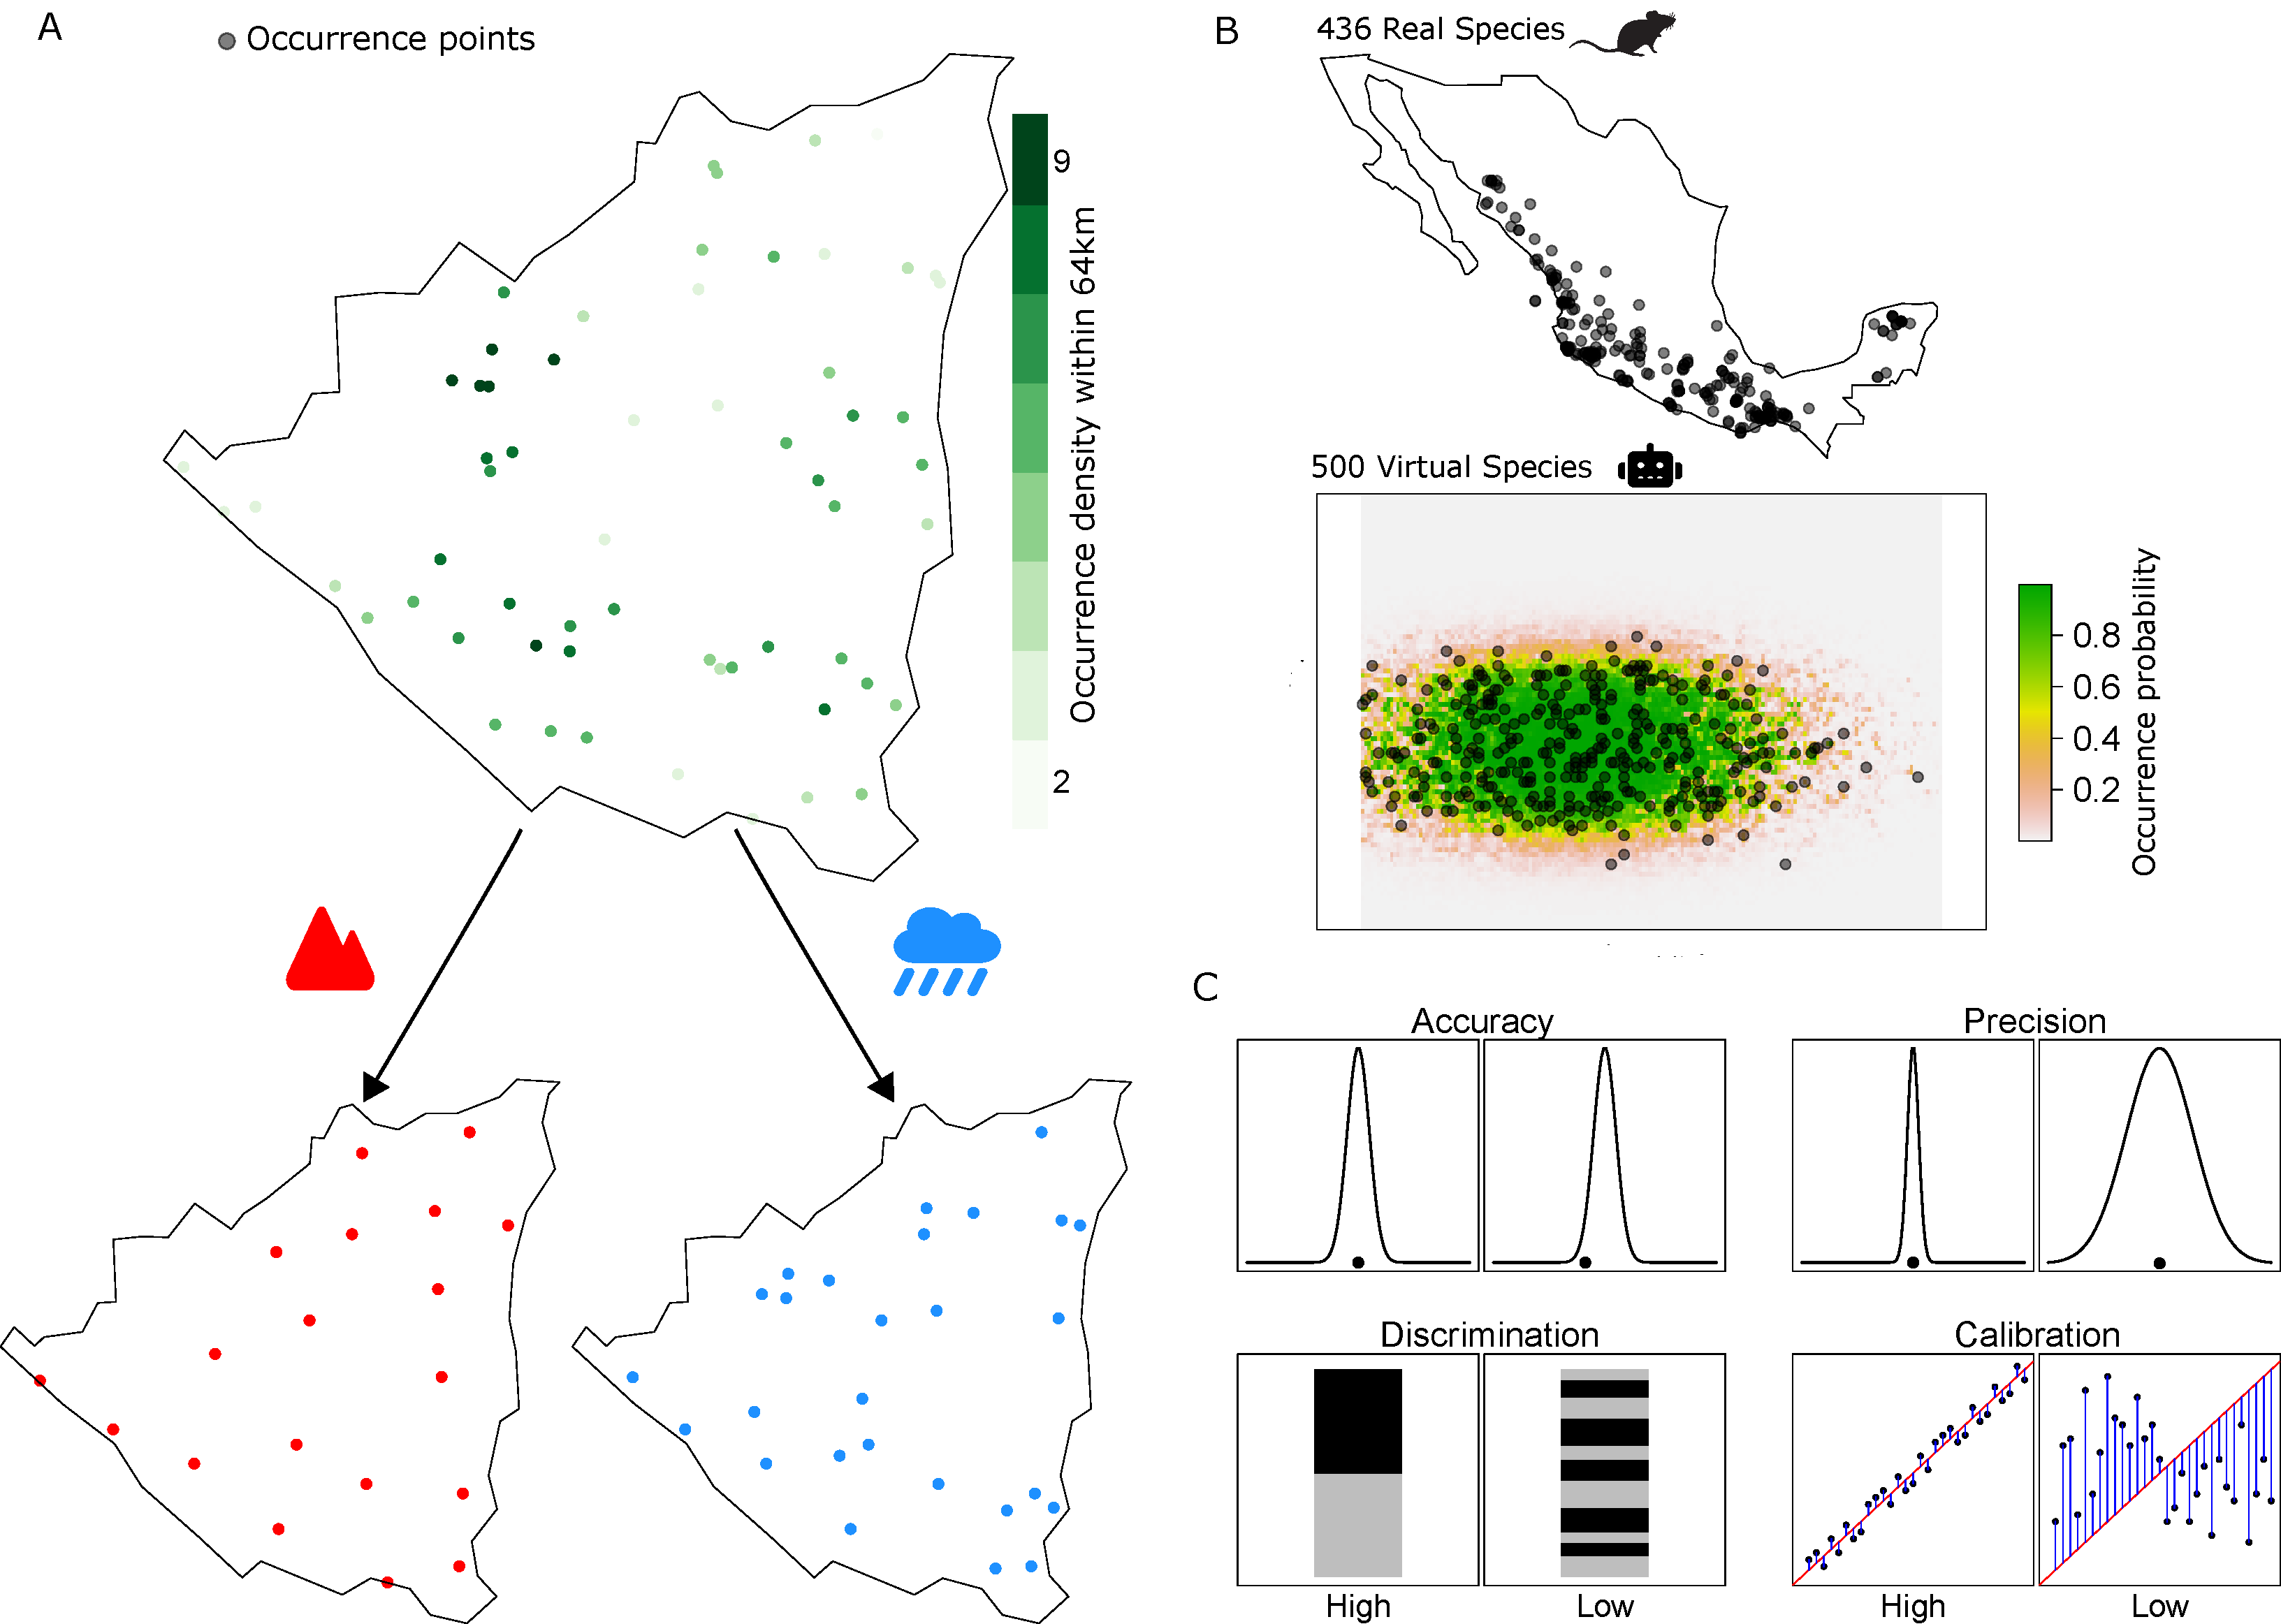
\includegraphics[width=1\textwidth]{Plots/Teste}}
\caption[Thinning occurrence data]{An example of how spatial (red mountain) and environmental (blue cloud) thinning can lead to a selection of different sets of occurrence points that are used to model the species distributions and that could influence model performance measures.}
\label{fig:concep_sdmthin}
\end{figure}
  

\begin{figure}[H]
\centering
%\graphicspath{ {c:/Teste/Chapter-1-Protocol/Manuscript/Plots/} }
\centerline{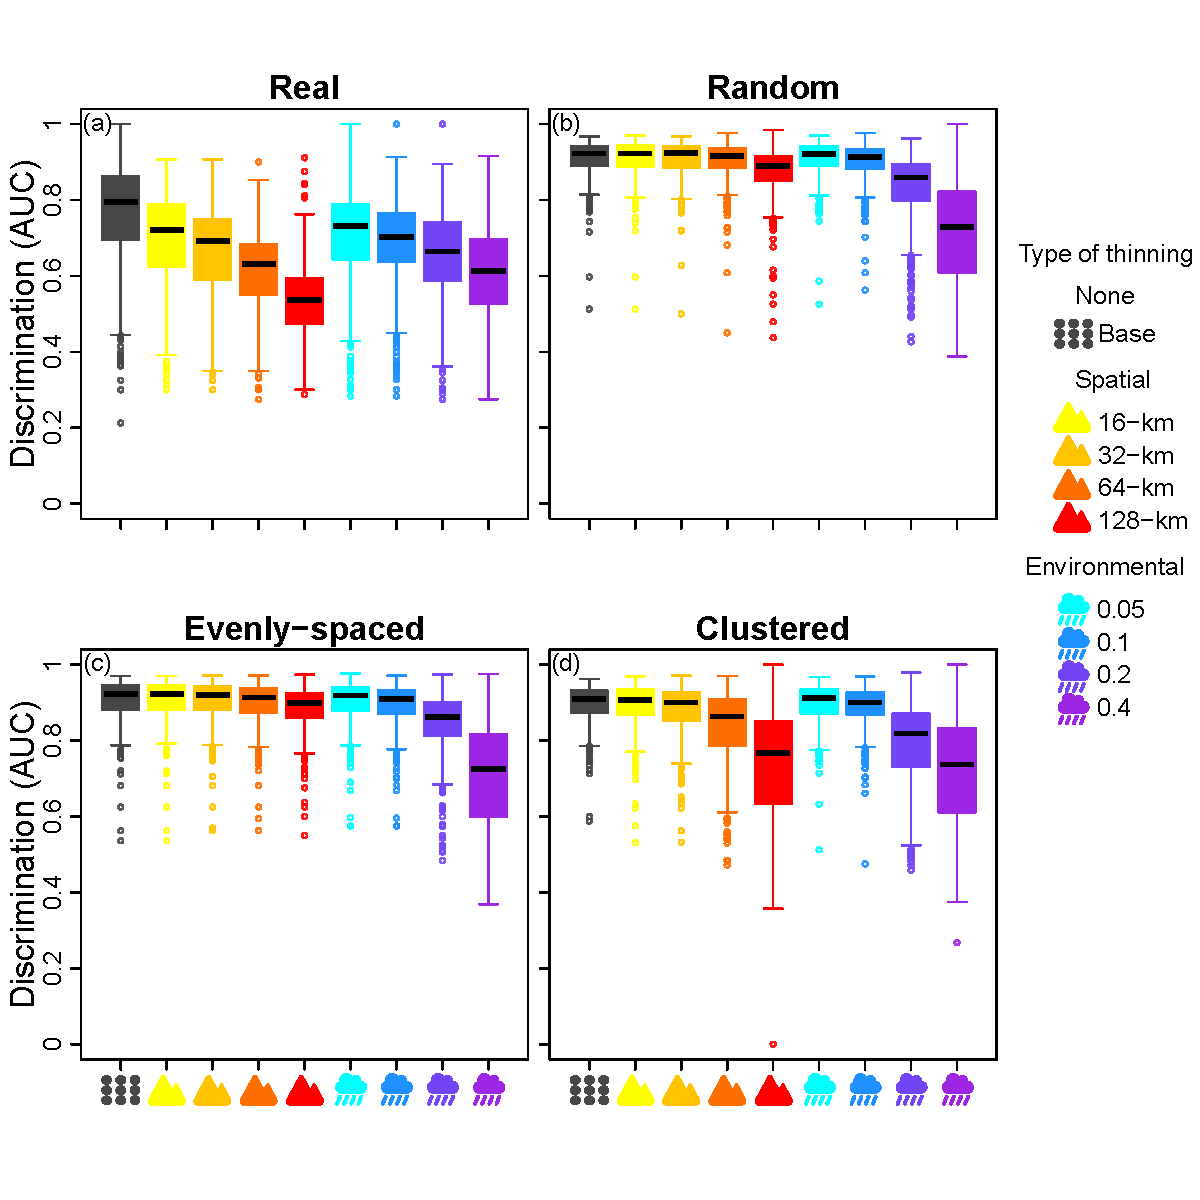
\includegraphics[width=1\textwidth]{Plots/Figure2}}
\caption[Effects of spatial and environmental thinning on model performance]{The effects of spatial and environmental thinning on MaxEnt discrimination (Area Under the Curve, AUC) for real species (a), and virtual species with random (b), evenly-spaced (c), and clustered (d) sampled occurrence points. }
\label{fig:Figure2}
\end{figure}

\begin{figure}[H]
\centering
%\graphicspath{ {c:/Teste/Chapter-1-Protocol/Manuscript/Plots/} }
\centerline{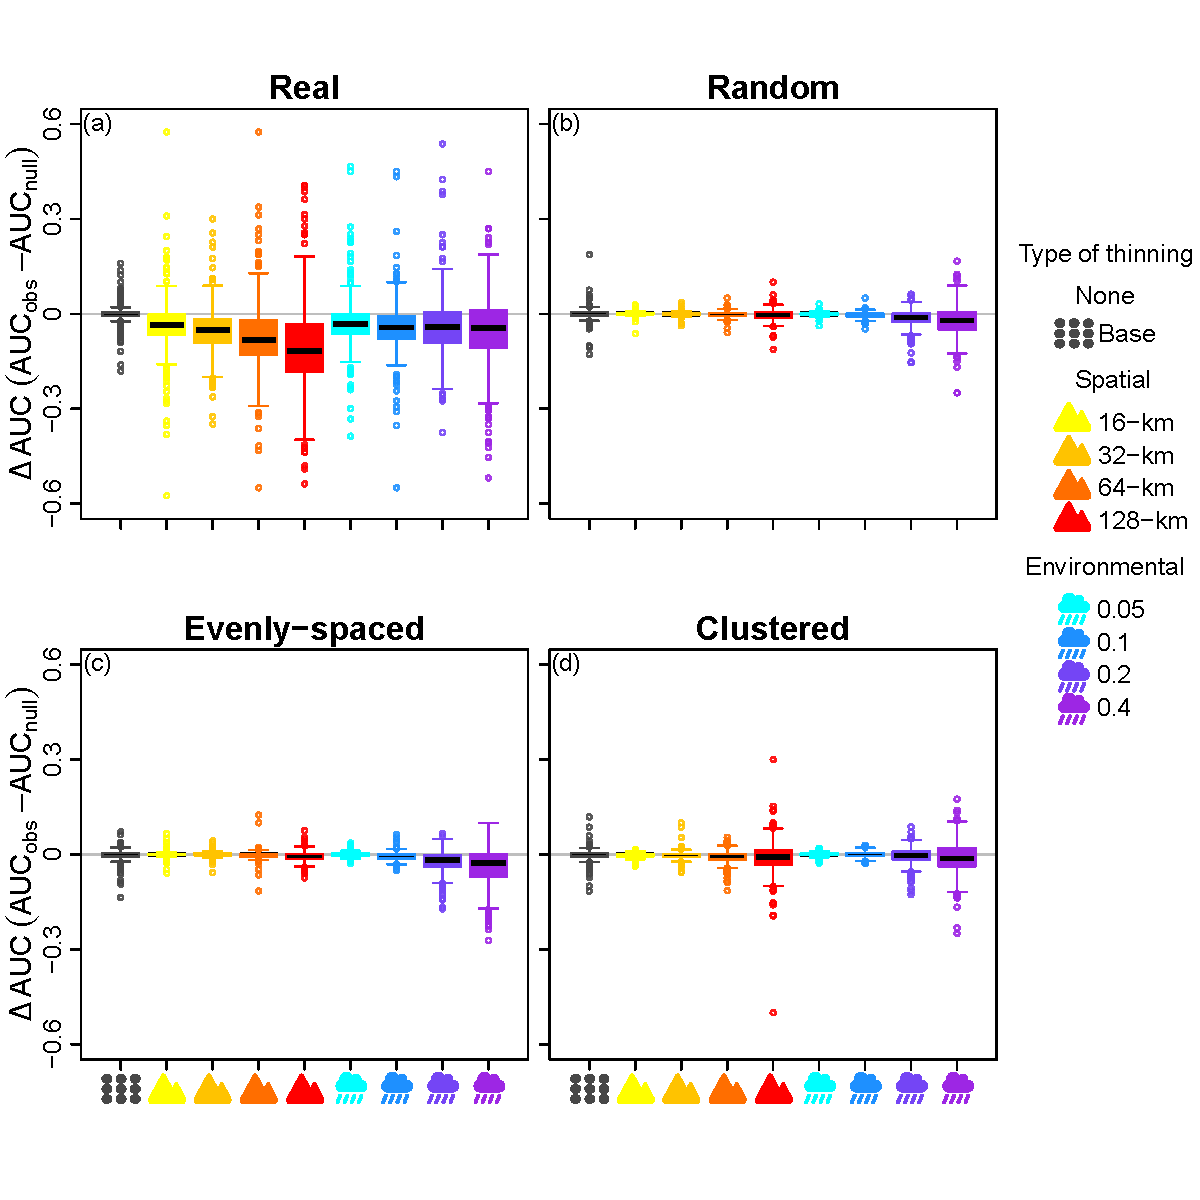
\includegraphics[width=1\textwidth]{Plots/Figure3}}
\caption[Model performance of thinned and null data]{Differences in discrimination (Area Under the Curve (AUC), $\Delta$AUC) of models trained with thinned (AUC$_{obs}$) and null (AUC$_{null}$) data for real species (a), and virtual species with random (b), evenly-spaced (c), and clustered (d) sampled occurrence points.} 
\label{fig:Figure3}
\end{figure}


\begin{figure}[H]
\centering
%\graphicspath{ {c:/Teste/Chapter-1-Protocol/Manuscript/Plots/} }
\centerline{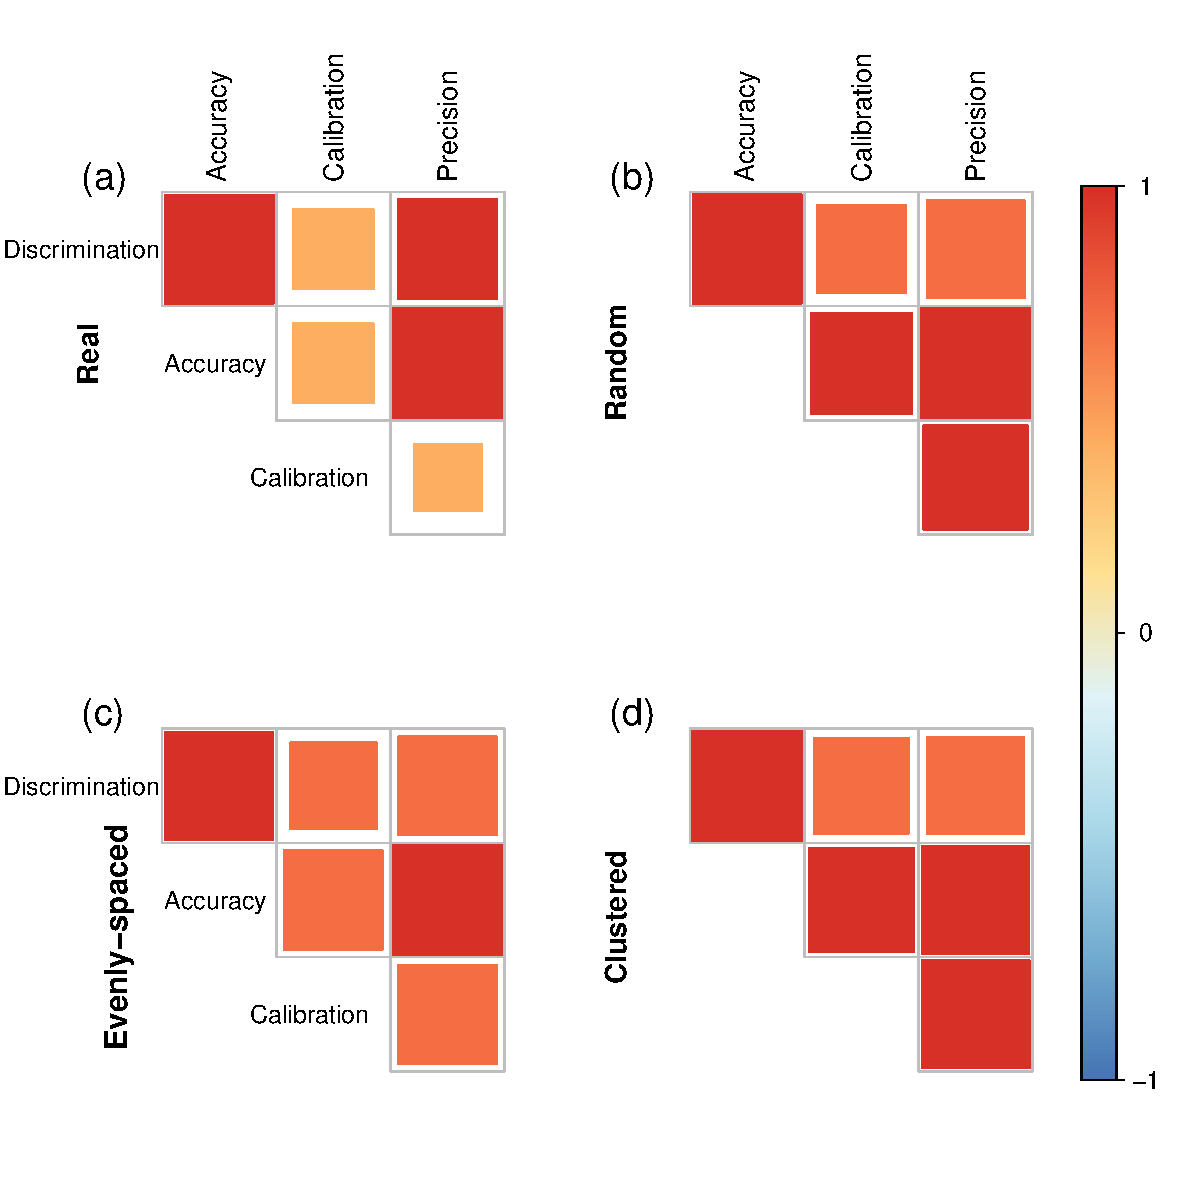
\includegraphics[width=1\textwidth]{Plots/Figure4}}
\caption[Correlation between performance metrics]{Correlation between the performance metrics for real species (a), and virtual species with random (b), evenly-spaced (c), and clustered (d) sampled occurrence points.}
\label{fig:Figure4}
\end{figure}

\section*{\textbf{\underline{Tables}}}
\begin{table}[H]
\centering
\caption[Results from linear mixed effect models]{Fitted linear mixed effects models showing the negative effects of thinning on SDM discrimination (Area Under the Curve, AUC) for real and virtual species with random, evenly-spaced and clustered spatial bias in sampled occurrence points. Significant results ($p$ < 0.05 are highlighted in bold).}
\begin{tabular}{ccccccc}
  \hline
Species & Thinning & Estimate & SE & d.f. & t & p-value \\ 
  \hline
\multirow{8}{*}{\rotatebox{90}{Real}} & S-16 & -0.067 & 0.005 & 3444.2 & -14.464 & \textbf{<0.001} \\ 
   & S-32 & -0.099 & 0.005 & 3444.3 & -21.416 & \textbf{<0.001} \\ 
   & S-64 & -0.152 & 0.005 & 3444.5 & -32.818 & \textbf{<0.001} \\ 
   & S-128 & -0.229 & 0.005 & 3445.0 & -49.289 & \textbf{<0.001} \\ 
   & E-10 & -0.060 & 0.005 & 3443.9 & -12.954 & \textbf{<0.001} \\ 
   & E-15 & -0.076 & 0.005 & 3443.9 & -16.490 & \textbf{<0.001} \\ 
   & E-20 & -0.107 & 0.005 & 3444.3 & -23.269 & \textbf{<0.001} \\ 
   & E-25 & -0.158 & 0.005 & 3444.4 & -34.147 & \textbf{<0.001} \\\hline 
   \multirow{8}{*}{\rotatebox{90}{Random}} & S-16 & -0.000 & 0.003 & 3992.0 & -0.018 & 0.986 \\ 
   & S-32 & -0.001 & 0.003 & 3992.0 & -0.376 & 0.707 \\ 
   & S-64 & -0.008 & 0.003 & 3992.0 & -2.245 & \textbf{0.025}\\ 
   & S-128 & -0.034 & 0.003 & 3992.0 & -10.078 & \textbf{<0.001} \\ 
   & E-10 & -0.002 & 0.003 & 3992.0 & -0.498 & 0.619 \\ 
   & E-15 & -0.009 & 0.003 & 3992.0 & -2.704 & \textbf{0.007}\\ 
   & E-20 & -0.076 & 0.003 & 3992.0 & -22.641 & \textbf{<0.001} \\ 
   & E-25 & -0.196 & 0.003 & 3992.0 & -58.002 & \textbf{<0.001} \\\hline 
   \multirow{8}{*}{\rotatebox{90}{Evenly-spaced}} & S-16 & -0.001 & 0.003 & 3992.0 & -0.174 & 0.862 \\ 
  & S-32 & -0.003 & 0.003 & 3992.0 & -1.012 & 0.312 \\ 
  & S-64 & -0.008 & 0.003 & 3992.0 & -2.683 & \textbf{0.007} \\ 
  & S-128 & -0.021 & 0.003 & 3992.0 & -6.975 & \textbf{<0.001}\\ 
  & E-10 & -0.004 & 0.003 & 3992.0 & -1.296 & 0.195 \\ 
  & E-15 & -0.014 & 0.003 & 3992.0 & -4.697 & \textbf{<0.001} \\ 
  & E-20 & -0.061 & 0.003 & 3992.0 & -20.122 & \textbf{<0.001} \\ 
  & E-25 & -0.197 & 0.003 & 3992.0 & -65.381 & \textbf{<0.001} \\\hline 
   \multirow{8}{*}{\rotatebox{90}{Clustered}} & S-16 & -0.002 & 0.004 & 3992.0 & -0.379 & 0.704 \\ 
   & S-32 & -0.013 & 0.004 & 3992.0 & -3.164 & \textbf{0.002} \\ 
   & S-64 & -0.058 & 0.004 & 3992.0 & -13.672 &\textbf{<0.001}\\ 
   & S-128 & -0.155 & 0.004 & 3992.0 & -36.414 & \textbf{<0.001}\\ 
   & E-10 & 0.003 & 0.004 & 3992.0 & 0.739 & 0.460 \\ 
   & E-15 & -0.006 & 0.004 & 3992.0 & -1.410 & 0.159 \\ 
   & E-20 & -0.101 & 0.004 & 3992.0 & -23.732 & \textbf{<0.001}\\ 
   & E-25 & -0.175 & 0.004 & 3992.0 & -41.116 & \textbf{<0.001}\\ 
   \hline
\end{tabular} 
\label{tab:LMMtable}
\end{table}



















                         %% Introduction.tex should begin

%\include{Squares}         %% The three sections of Chapter 1 
%\input{Cube}             %% are in the files Squares.tex,  
%\input{Hypercubes}	   %% Cubes.tex and Hypercubes.tex

%\addtocontents{lof}{\protect\vskip-50pt}
\addtocontents{toc}{\protect\vskip-20pt}
\chapter[Demography and dispersal influence the relationship between habitat suitability and population density.]{Demography and dispersal influence the relationship between habitat suitability and population density.\footnote[2]{Submitted to \textit{Ecography} as: Ten Caten, C., \& T. Dallas. Demography and dispersal influence the relationship between habitat suitability and population density.}}


\section*{\textbf{\underline{Abstract}}}
A central goal of ecology is to understand spatial patterns of species densities. Habitat suitability estimates from species distribution models (SDMs) could be used to represent species density and overcome the scarcity of density data. However, there is mixed evidence that habitat suitability relates to density, and it is suggested that local dynamics affect the relationship between habitat suitability and density. We simulated population dynamics for 200 virtual species with different combinations of factors (demographic stochasticity, dispersal, and intraspecific competition) that affect population sizes and trained SDMs considering different sets of environmental predictors to evaluate when habitat suitability reflected densities. We found that even when population growth rate and demographic stochasticity are the only factors driving population dynamics habitat suitability was not consistently related to species densities. Incorporating dispersal dynamics and spatial differences in intraspecific competition had small negative effects on the relationship between habitat suitability and density, showing that these factors influence these relationships. Species differences partially explained the variability in the relationship between habitat suitability and density across species. Similar results were found for 200 North American bird species, indicating that habitat suitability estimates from SDMs should not be used to understand species densities.

%-----------------------
\section*{\textbf{\underline{Introduction}}}
%\section*{Introduction}

The fundamental niche is a persistence threshold that defines the sets of environmental conditions that allows species to persist across geographic space \parencite{hutchinson1957,pulliam2000, colwell2009}. Several statistical methods that relate species occurrence data with environmental conditions have been developed to identify areas that are environmentally suitable for species occurrence \parencite{peterson2011}. These tools, frequently referred to as species distribution models (SDMs), are primarily used to estimate species geographic distributions and have been essential for answering macroecological and biogeographical questions as well as to aid conservation efforts \parencite{cayuela2009, calabrese2014,biber2020}. SDMs generate habitat suitability estimates where higher values represent more favorable conditions for species to occupy. These favorable conditions are usually assumed to support larger population sizes because of an increased survival and reproductive success of individuals occurring in these areas \parencite{weber2017,dallas2018,lee2022}, leading to a potential positive relationship between habitat suitability and species abundance \parencite{gomes2018}. In this case, \textit{density} (number of individuals per area) is perhaps the more appropriate term than abundance, as oftentimes it is the only possible measure. 


\paragraph*{}
This putative relationship between habitat suitability and density has spurred an interest in using SDMs to predict species densities \parencite{oliver2012sdm,acevedo2017,corbel2023}. Estimating species density through sampling approaches is a difficult task, such that a lack of spatial and temporal density data, a shortcoming called the \textit{Prestonian shortfall}, represents a major knowledge gap for most species \parencite{hortal2015}. Addressing this knowledge gap is important given that having information on species densities is crucial for understanding population dynamics. Using SDMs to predict species density is thus compelling given the more widespread availability of presence data that are often used in these models \parencite{pearce2006, bradley2016}. However, current evidence indicates that SDMs have limited efficacy in describing species density as most successful predictions come from cases where these relationships were assessed for single species whereas evaluations considering multiple species tend to be unsuccessful \parencite{weber2017,dallas2018,lee2022, waldock2022}.



\paragraph*{}
A lack of connection between habitat suitability and density could occur because a species density in a given location is affected by factors that are often ignored in SDMs \parencite{boulangeat2012}. For example, spatial differences in the level of intraspecific competition, because of differences in resource availability, can lead to complex spatial patterns of population dynamics \parencite{klomp1964, turnbull2007, zhang2021}. Dispersal can further affect observed population densities by allowing the persistence of populations in unsuitable environments through source-sink dynamics \parencite{pulliam1988,pulliam2000,furrer2016}. Moreover, when there are spatial differences in population growth rates and in intraspecific competition, dispersal can enhance population sizes and lead to larger than expected populations \parencite{oksanen1990,zhang2021}. When population sizes are small, demographic stochasticity plays an important role in driving population dynamics where these populations can face a higher extinction risk \parencite{gabriel1992,melbourne2008}. Since SDMs are trained on binary data and assume equilibrial dynamics, it can be particularly challenging for habitat suitability estimates to relate to species densities given the several factors, such as the ones outlined above, that affect population sizes.  
 
 

\paragraph*{}
Species tolerate different ranges of environmental conditions and use different types of resource, which could further lead habitat suitability estimates to be unrelated to density. For example, abundance-occupancy relationships describe the tendency for widespread species to be more locally abundant than restricted species, possibly because these widespread species are more generalist in terms of environmental conditions they tolerate or in the resources they use \parencite{borregaard2010,ten2022}. For such generalist species, SDMs might not be able to detect important environmental variables that limit their distributions, making these models unable to differentiate suitable and unsuitable environments in these cases \parencite{hernandez2006, van2016, harisena2021}. Conversely, species with restricted distributions can still achieve high densities in locations they occupy depending on local resource availability \parencite{komonen2009, crisfield2024}. As species might exhibit different types of specialization that can lead to complex patterns of geographic distributions and densities \parencite{crisfield2024}, SDMs might have difficulties distinguishing these types of specialization from occurrence data. Lastly, species can have performance curves (i.e., the relationship between how population growth rate changes along environmental conditions) with different characteristics that SDMs might also not be able to properly describe from occurrence data, which would ultimately render these models inappropriate for understanding densities \parencite{lee2022}.
 
\paragraph*{}
Here, we used a simulation framework to examine the effects of incorporating demographic stochasticity, dispersal, and intraspecific competition when modeling population dynamics across geographic space on the relationship between habitat suitability and density (Figure \ref{fig:conce_sdmabnd}). Simulated species had performance curves of different shapes and breadth to consider how species differences affect these relationships. To examine the generalities of these relationships in nature we also assessed how habitat suitability related to the density of 200 North American bird species. We found that habitat suitability was often positively correlated to density, but these relationships were highly variable and habitat suitability often explained $\approx 25\%$ and $\approx 5\%$ virtual species and North American birds densities, respectively. Demographic stochasticity, dispersal, and intraspecific competition had small negative effects on these relationships, and species differences and characteristics of the SDMs explained a small amount of the variability in these relationships across virtual species, suggesting that habitat suitability often does not reflect species densities.
 
%-----------------------
\section*{\textbf{\underline{Methods}}}
%\section*{Methods}
\paragraph*{Virtual species population dynamics}\mbox{}\\
We simulated 200 virtual species occurring in a lattice representing the United States and Canada (spatial resolution of 20 minutes that had 25207 cells, Figure \ref{fig:NA_prec}) using population models that considered different factors that influence population dynamics (Figure \ref{fig:conce_sdmabnd}). A discrete time Ricker model was used to simulate population dynamics, where populations grew according to population growth rate $R$ and intraspecific competition ($\alpha = 0.005$) limited population sizes. The number of offspring was treated as a Poisson random variable with mean of \textit{R} offspring per individual and survivorship was treated as a Binomial random variable with probability $e^{- \alpha N_{t}}$, representing the effects of demographic stochasticity in our model. 

\begin{equation}
\label{eq:ricker}
N_{t+1} = N_{t} \ R \ e^{- \alpha N_{t}}
\end{equation}  

In this model demographic stochasticity and population growth rate were the only factors causing changes in population sizes across generations. This model was expanded to also allow the occurrence of dispersal events between populations following a binomial random variable with probability $d$ ($d = 0.20$). Individuals dispersing from a focal population immigrated to new populations according to a negative exponential dispersal kernel \parencite{nathan2012} that was species-specific (Figure \ref{fig:kernel}). The maximum dispersing distance (in number of cells) was randomly chosen between 5 and 25 and the mean dispersal distance was a randomly chosen fraction between 0.1 and 0.6 of the maximum dispersal distance. Individuals could not disperse to cells outside the borders of the lattice (Figure \ref{fig:kern_crop}). This model was further expanded to allow spatial variation in the strength of intraspecific competition \parencite{zhang2021}. We used data on productivity to inform the intensity of intraspecific competition as productivity limits population and community sizes of several taxa \parencite{srivastava1998,cerezer2021}. We assumed a linear negative relationship between the productivity of a site and the level of intraspecific competition that a given population experienced ($\alpha = 0.005 - 0.1$). We used the normalized difference vegetation index (NDVI) as a proxy for productivity and we obtained NDVI data for the first day of June of 2020 from MODIS through the R package \texttt{MODIStsp} \parencite{busetto2016}. 

For each species, populations were simulated considering the following combination of factors: demographic stochasticity (considered our baseline model), demographic stochasticity and spatial intraspecific competition, demographic stochasticity and dispersal, and  demographic stochasticity, spatial intraspecific competition, and dispersal, resulting in four population simulations per species. Simulations started with all cells in the lattice occupied with 20 individuals from a given species and models ran for a total of 100 generations to allow population dynamics to reach equilibrium. By the end of the simulations, occupancy (fraction of occupied cells in the lattice) varied across species (0.38 $\pm$ 0.16), and we sampled 100-750 of those occupied cells to model the distribution of virtual species. We chose this number of cells for the virtual species to be consistent with the number of sites that the North American bird species considered in our study occupied (see below).   
 
Two performance curves, a symmetric and an asymmetric, were simulated for each virtual species considering mean annual temperature in the United States and Canada (see details in the \textit{Environmental predictors and model structure} section below). We simulated performance curves considering mean annual temperature because there is significant spatial variation in temperature patterns in North America (Figure \ref{fig:NA_prec}). Mean annual temperature values ranged $-$26$^{\circ}$C to 24.4 $^{\circ}$C, allowing the possibility of simulating species that tolerate different ranges of temperatures. Symmetric and asymmetric performance curves were used because several species have performance curves with these properties \parencite{oksanen2002, vasseur2014}. These performance curves represent how species' population growth rates change along temperature gradients, and they were used to estimate \textit{R} of each population occurring in a given location. We used the \textit{sech} function available in the \texttt{senlm} package \parencite{anderson2022} to simulate symmetric and asymmetric performance curves. A species had the same optimum temperature (location of the maximum, $m$ parameter in \textit{sech}) for both performance curves, and this optimum was randomly sampled between -15 and 14. However, curves differed in skewness (symmetry, $r$, parameter), where the skewness of the symmetric and asymmetric curves was  0 and -0.95, respectively. A negative value of skewness makes the performance curve have a broader left-hand tail while a value of 0 makes the performance curve symmetric \parencite{anderson2022}. Peakedness (peakedness, $p$, parameter) was chosen to be 3 and 5.25 for symmetric and asymmetric curves, respectively. The peakedness parameter controls the kurtosis of the performance curve and smaller values lead to flatter curves where population growth rates decrease more slowly away from the optimum environmental condition. Lastly, the spread (spread, $s$, parameter) of the asymmetric curves was $1/3$ of the spread of symmetric curves. The spread represents the range of temperature values that a species could tolerate, and these values were randomly sampled between 3 and 10. Our goal was to evaluate whether the shape and the breadth of a species performance curve could affect the relationship between habitat suitability and density. Figure \ref{fig:curves} shows an example of how a symmetric and an asymmetric performance curves change along the temperature gradient for a species. 

\paragraph*{North American bird density data}\mbox{}\\
We used data on North American bird species to compare habitat suitability estimates from SDMs to the density of these species to explore the generality of these relationships for real species. Bird density data were obtained from the Breeding Bird Survey (BBS; \textcite{sauer2020}). The BBS is a yearly standardized census of North American bird species that is performed by volunteers during the breeding season. In these surveys, routes of $\approx$ 50km are sampled every 1km for about three minutes through point counts where all birds seen or heard within a radius of 0.4 km are recorded. We used the data sampled from 1997-2019 to estimate the mean annual density and to model the distribution of 200 bird species that were observed occurring in 100-750 locations. We chose this temporal extent to calculate mean annual density because a consistent number of sites ($\approx$ 3000) have been continuously sampled by BBS since 1997, providing reliable estimates of population density for this time period. Incomplete sampling and detection probability could affect where species are recorded and their observed density and potentially influence the analyses of such data. However, incomplete sampling should not affect our study given the standardized nature of how the BBS data are collected, and also because there is limited evidence for potential biases influencing analyses of the BBS data across large spatial and temporal scales considering several species \parencite{rosenberg2019}. Moreover, the effects of detection probability are more prevalent when population sizes are small \parencite{tanadini2011, bennett2024}, such that both occurrence (used in SDMs to estimate habitat suitability) and density (used to relate to habitat suitability) data would be similarly affected by detection probability in these cases. This suggests that incomplete sampling or detection probability should have not influenced the relationship between habitat suitability and density that we observed for North American birds.

\paragraph*{Environmental predictors and model structure}\mbox{}\\
We obtained the 19 bioclimatic variables available in WorldClim 2.1 at a resolution of 10 minutes through the \texttt{geodata} R package \parencite{fick2017, geodata}. These variables include different measurements of temperature and precipitation patterns that are considered important determinants of species distributions \parencite{barbet2014, illan2014}. For the North American bird species, we performed a PCA over the 19 bioclimatic variables covering North America and used the first four axes as predictors to model the species distributions given that they explained over 90\% of the variation in the data \parencite{kriticos2014}. These environmental predictors were aggregated to have a resolution of 30 minutes when modeling the distribution of North American birds to match the spatial resolution in which the BBS data is sampled.  

The distribution of virtual species were modeled using different sets of environmental predictors. First, we modeled their distributions using mean annual temperature and NDVI as predictors. This represents a situation where there is a perfect knowledge about the environmental conditions that affect the population dynamics of species. SDMs were fitted using NDVI and mean mean annual temperature as predictors for the four population models that we considered. We also modeled species distributions using mean annual temperature, mean diurnal range in temperature, temperature seasonality, annual precipitation, precipitation of the wettest month, and precipitation seasonality (hereafter multiple environmental predictors). This exemplifies a situation where there is some knowledge about what variables potentially affect population dynamics, but unimportant predictors are also considered in the model. SDMs using these multiple environmental predictors were fitted for population models that simultaneously considered demographic stochasticity, spatial intraspecific competition, and dispersal. Lastly, we performed a principal components analysis (PCA) over these 19 bioclimatic variables covering the United States and Canada and used the first four axes that explained over 90\% of the variance of the data as predictors in the model. This constitutes a case where there is limited or no knowledge about the environmental factors that affect the population dynamics of a given species. SDMs using these PCA axes as predictors were also fitted for population models that simultaneously considered demographic stochasticity, spatial intraspecific competition, and dispersal. Thus, we were able to examine whether SDMs trained with uninformative environmental predictors had habitat suitability estimates that were less related to density. Environmental variables were aggregated to have a spatial resolution of 20 minutes when modeling the distribution of the virtual species to match the resolution in which their population dynamics were simulated. 

\paragraph*{Modeling and evaluating species distributions}\mbox{}\\
The distribution of virtual and real species was modeled using MaxEnt, a widely used machine-learning method that requires presence and pseudo-absence data and that generally have good performance \parencite{elith2010, santini2021}. Models were fit using default regularization coefficient values as these have been shown to perform well for a wide range of species and because fine tuning models individually for each species is impractical when considering several species as in our case \parencite{phillips2008, merow2013}. Prevalence of presences and pseudo-absences was kept at 0.5, where 50\% of the data used are presences and 50\% are pseudo-absences \parencite{senay2013, iturbide2015}. Pseudo-absences were randomly sampled from a 400km buffer surrounding presence points of virtual and real species. We used a cross-validation procedure, where 75\% of our dataset was used to train the models and the other 25\% was used to test the models. This process was repeated 20 times to account for potential differences in the habitat suitability estimates that could arise from using specific sets of presences and pseudo-absences when training and testing the models. Models were evaluated using the area under the receiver operating characteristic curve (AUC) \parencite{fielding1997}. AUC is a discrimination performance measure that assesses how well a model distinguishes between presences and pseudo-absences, where values closer to 1 suggests a model is good at differentiating presences from pseudo-absences and values around 0.5 indicates a random performance. Habitat suitability estimates and AUC were averaged across species considering the 20 models that were fitted for each species. For the virtual species, we assessed whether habitat suitability estimates produced by SDMs could replicate their performance curves. Performance curves were rescaled to 0-1 and we compared, along the temperature gradient, the difference between observed mean habitat suitability produced by SDMs and the actual population growth rate in a given environment based on the performance curve of the species.




\paragraph*{Assessing the relationship between habitat suitability and density}\mbox{}\\
The presence data used to model species distributions were used to evaluate how habitat suitability related to species density.  We extracted habitat suitability for each presence point, and we used the observed population size to represent species densities in those locations. The relationship between habitat suitability and density was evaluated using Pearson's correlations. To examine how well habitat suitability explained density, we calculated the coefficient of determination, which is equal to the squared Pearson's correlation coefficient. 

We fitted two linear mixed-effect models to evaluate the effects of different factors on the relationship between habitat suitability and density across species. In both LMMs, we used the correlation coefficient ($r$) between habitat suitability and density as the response variable and species were used as random effects, but different fixed effects were considered. In our first LMM, our goal was to understand how factors that contribute to local population dynamics affect the relationship between habitat suitability and density. We encoded dummy variables to assess how considering dispersal and spatial intraspecific competition in population models affected these relationships. Demographic stochasticity was present in all models and was considered our baseline case. Thus, we did not encode a dummy variable for demographic stochasticity. In this LMM, we also considered whether using multiple environmental predictors or PCA axes when training SDMs affected the relationship between habitat suitability and density by encoding dummy variables for these predictors. In our second LMM, we were interested in understanding how species differences and SDMs characteristics could affect the relationship between habitat suitability and density. Fixed effects considered were the breadth and the shape (i.e., symmetric or asymmetric) of species performance curves, the mean absolute difference between habitat suitability and population growth rate (estimated from presences), and the mean SDM performance. In this model, continuous predictors were in different scales and they were standardized to allow comparisons of their effects on the relationship between habitat suitability and density. LMMs were fit using the \texttt{glmmTMB} R package \parencite{brooks2017} while model diagnostics (models assumptions were genrally met; see Figures \ref{fig:mod_dyn}-\ref{fig:mod_sp} and Appendix B for details) and goodness of fit (Nakagawa's conditional $R^2$) were estimated using the \texttt{performance} R package \parencite{ludecke2021}. This conditional $R^2$ takes fixed and random effects into account when estimating the model goodness of fit. 
%-----------------------
\section*{\textbf{\underline{Results}}}
%\section*{Results}


\paragraph*{Do demographic stochasticity, dispersal, and intraspecific competition affect the relationship between habitat suitability and density?}\mbox{}\\
Correlations between habitat suitability and density were often significant and positive, but the strength of these relationships varied considerably across species within the different models of population dynamics (Figure \ref{fig:cor}a), and habitat suitability explained $\approx$ 25\% of the variation in species density (Figure \ref{fig:cor}b). Habitat suitability was not consistently related to density even when population dynamics were driven solely by population growth rates and demographic stochasticity and SDMs were trained with the two environmental factors that affected the density of species. We found that in the baseline case (the intercept) of our first LMM, the average correlation between habitat suitability and density was 0.48. This correlation is reduced to 0.45 for population models that considered dispersal ($\beta = -0.027$, $p < 0.01$) and to 0.41 for models that considered spatial differences in intraspecific competition ($\beta = -0.069$, $p < 0.01$; Figure \ref{fig:cor}c). Nakagawa's conditional $R^2$ was 0.28, indicating that this LMM had a relatively limited explanatory power. The performance of SDMs widely varied across virtual species, such that these models tended to have lower performance for species that have broader performance curves (see Appendix B and Figure \ref{fig:auc}).


SDMs were more consistently able to identify the important environmental predictor that drives population growth rate when they were trained with mean annual temperature and NDVI than when multiple environmental predictors were considered (Figure \ref{fig:imp}). However, using multiple environmental predictors had no effect on the correlation between habitat suitability and density, while using PCA axes as predictors negatively affected these relationships ($\beta = -0.099$, $p < 0.01$; Figure \ref{fig:cor}c). This suggests that having no information on environmental factors that affect population dynamics may lead to habitat suitability estimates that are less related to species densities.


\paragraph*{What explains the high variability in the relationship between habitat suitability and density?}\mbox{}\\
We found that the high variability in the relationship between habitat suitability and density observed across virtual species could be explained by some of the factors that we considered in our second LMM. The baseline case (the intercept) of this LMM had an average correlation between habitat suitability and density of 0.39. Habitat suitability tended to relate less to the density of species that had broader performance curves ($\beta = -0.039$, $p < 0.01$; Figure \ref{fig:diff}a, e) or when habitat suitability poorly reflected population growth rates ($\beta = -0.061$, $p < 0.01$; Figure \ref{fig:diff}b, e). SDMs performance and the shape of species performance curves did not affect the relationship between habitat suitability and density (Figure \ref{fig:diff}c-e). Nakagawa's conditional $R^2$ was 0.20, also suggesting that this LMM could not explain most of the variation in the relationship between habitat suitability and density across species. 


\paragraph*{What is the relationship between habitat suitability and density for North American birds?}\mbox{}\\
We found that habitat suitability and density were positively correlated for 54\% of the North American birds, while negative and non-significant relationships were observed for 5.5\% and 40.5\% of the species, respectively (Figure \ref{fig:cor}a). Despite finding these positive relationships, habitat suitability rarely explained over $5\%$ of the variation in density of North American birds (Figure \ref{fig:cor}b). These results showed that habitat suitability is less often related to the density of real species compared to virtual species, and significant correlations could only explain a particularly small fraction of the variation in density of North American birds. Nevertheless, SDMs performed relatively well for North American birds (Figure \ref{fig:auc}). Overall, our results highlight a general disconnect between habitat suitability and species densities for virtual species and North American birds.








%-----------------------

\section*{\textbf{\underline{Discussion}}}
%\section*{Discussion}
We found that habitat suitability is often positively correlated to density, but these relationships were widely variable across species and had low explanatory power, indicating that habitat suitability estimates might be unreliable for understanding species densities. The disconnect between habitat suitability and density often reported for real species is usually attributed to the fact that several factors, such as dispersal dynamics or resource limitation, acting at the local scale could lead to complex spatial patterns of density that habitat suitability would be unable to capture \parencite{weber2017,dallas2018,jimenez2021}. We show that even when population growth rates and demographic stochasticity were the only factors influencing population sizes, habitat suitability estimates were still not consistently related to species densities. Incorporating dispersal dynamics and spatial intraspecific competition to our models had small negative effects on these relationships, showing that these factors influenced the relationship between habitat suitability and density. However, these findings also suggest that demography and dispersal may not be the main factors responsible for the weak link between habitat suitability and density. 

\paragraph*{}
The general disconnect between habitat suitability and density could occur because the presence data used to train SDMs might not contain the necessary information to describe densities. For example, high habitat suitability might suggest high probability of occurrence, but not of density, as environmental conditions can differently affect species occurrence and density \parencite{bradley2016}. SDMs that have poor performance and are unable to differentiate between presences and pseudo-absences are unlikely to be able to reflect densities altogether \parencite{jimenez2021}, but we observed that SDMs that had high performance did not produce habitat suitability estimates that were more closely related to density. This demonstrates that a model that is suitable for estimating occurrences does not necessarily translates into a model that is suitable for estimating densities. SDMs that produced habitat suitability estimates that more properly reflected population growth rates led to stronger correlations between habitat suitability and density across species. This occurs because these models provide a more accurate description of how species performances, and consequently the potential population size in a given area, change along environmental gradients. However, SDMs might be particularly unable to describe performance curves of species that tolerate a wide range of environmental conditions because these models often cannot discriminate suitable from unsuitable environments for such generalist species \parencite{hernandez2006,franklin2009,van2016}. This would explain why habitat suitability is less related to the density of species that have broader performance curves. 
 

\paragraph*{}
When assessed for a large number of mammals and plant species, the relationship between habitat suitability and density is often non-significant or is in contrasting directions \parencite{dallas2018,sporbert2020}. We also observed variable relationships between habitat suitability and density for the 200 North American birds species that we considered. The positive relationship between habitat suitability and density found for about half of the species we considered could be occurring because these birds might have higher dispersal ability and are more capable of tracking suitable environments across geographic space and over time \parencite{tingley2009, zurell2018}. This may occur through informed dispersal behavior where individuals would be more likely to disperse to good habitat patches \parencite{clobert2009, oro2021}. Alternatively, our simulations did not consider informed dispersal, which led to the occurrence of source-sink dynamics by allowing individuals to occupy unsuitable sites \parencite{pulliam1988, pulliam2000, furrer2016}. This could explain why dispersal had a negative effect on the relationship between habitat suitability and density of virtual species. Nonetheless, habitat suitability was still not able to explain most of the variation in the density of North American birds. This could be occurring because areas predicted to be of high environmental suitability can have populations of either low or high density \parencite{vanderwal2009, acevedo2017, braz2020}. Moreover, populations occurring in locations with low habitat suitability can still have positive growth rates \parencite{thuiller2014,cserg2017}, and potentially reach high densities, which could further obscure any potential relationship between habitat suitability and density. 


\paragraph*{}
Demographic stochasiticity, dispersal, and intraspecific competition affect local densities \parencite{melbourne2008,furrer2016, zhang2021}, but these factors seem to have played a limited role in driving the disconnect between habitat suitability and density in our simulations given their relatively small negative impacts on these relationships. However, it is likely that an interplay between different factors could lead to the general weaker, or lack of, relationship between habitat suitability estimates and density of real species. For example, interspecific competition and environmental stochasticity affect population densities \parencite{may1973, robertson1996} and could be interacting with the factors that we considered in our study to influence these relationships even more for real species \parencite{santini2019, braz2020}. The presence of sampling biases in the occurrence data that are often used to fit SDMs \parencite{inman2021,bowler2023}, alongside with the use of environmental conditions that might not be related to the population dynamics of species, such as PCA axes, may further increase the disconnect between habitat suitability and density for real species. 


\paragraph*{}
Using SDMs to predict species densities is compelling because the presence data used in these models are more readily available than density data \parencite{pearce2006, bradley2016, hortal2015}, but our findings suggest that SDMs should not be used for these purposes as they fail to describe different aspects of population dynamics under a wide range of scenarios. SDMs can still be useful for predicting species occurrences \parencite{lee2022}, but there is a growing body of evidence showing that their use to estimate densities should be avoided. Population densities in a given location is affected by a myriad of factors and using demographic models that are tailored specifically to predicting densities is a more productive path forward \parencite{dallas2018, lee2022}. Citizen-science databases that have count data could be used, for example, to test the predictions made by these demographic models and it could improve our understanding of population trends \parencite{dennis2017, fink2020}. 

\section*{\textbf{\underline{Figures}}}
%\section*{Figures}

\begin{figure}[ht]
\centering
\centerline{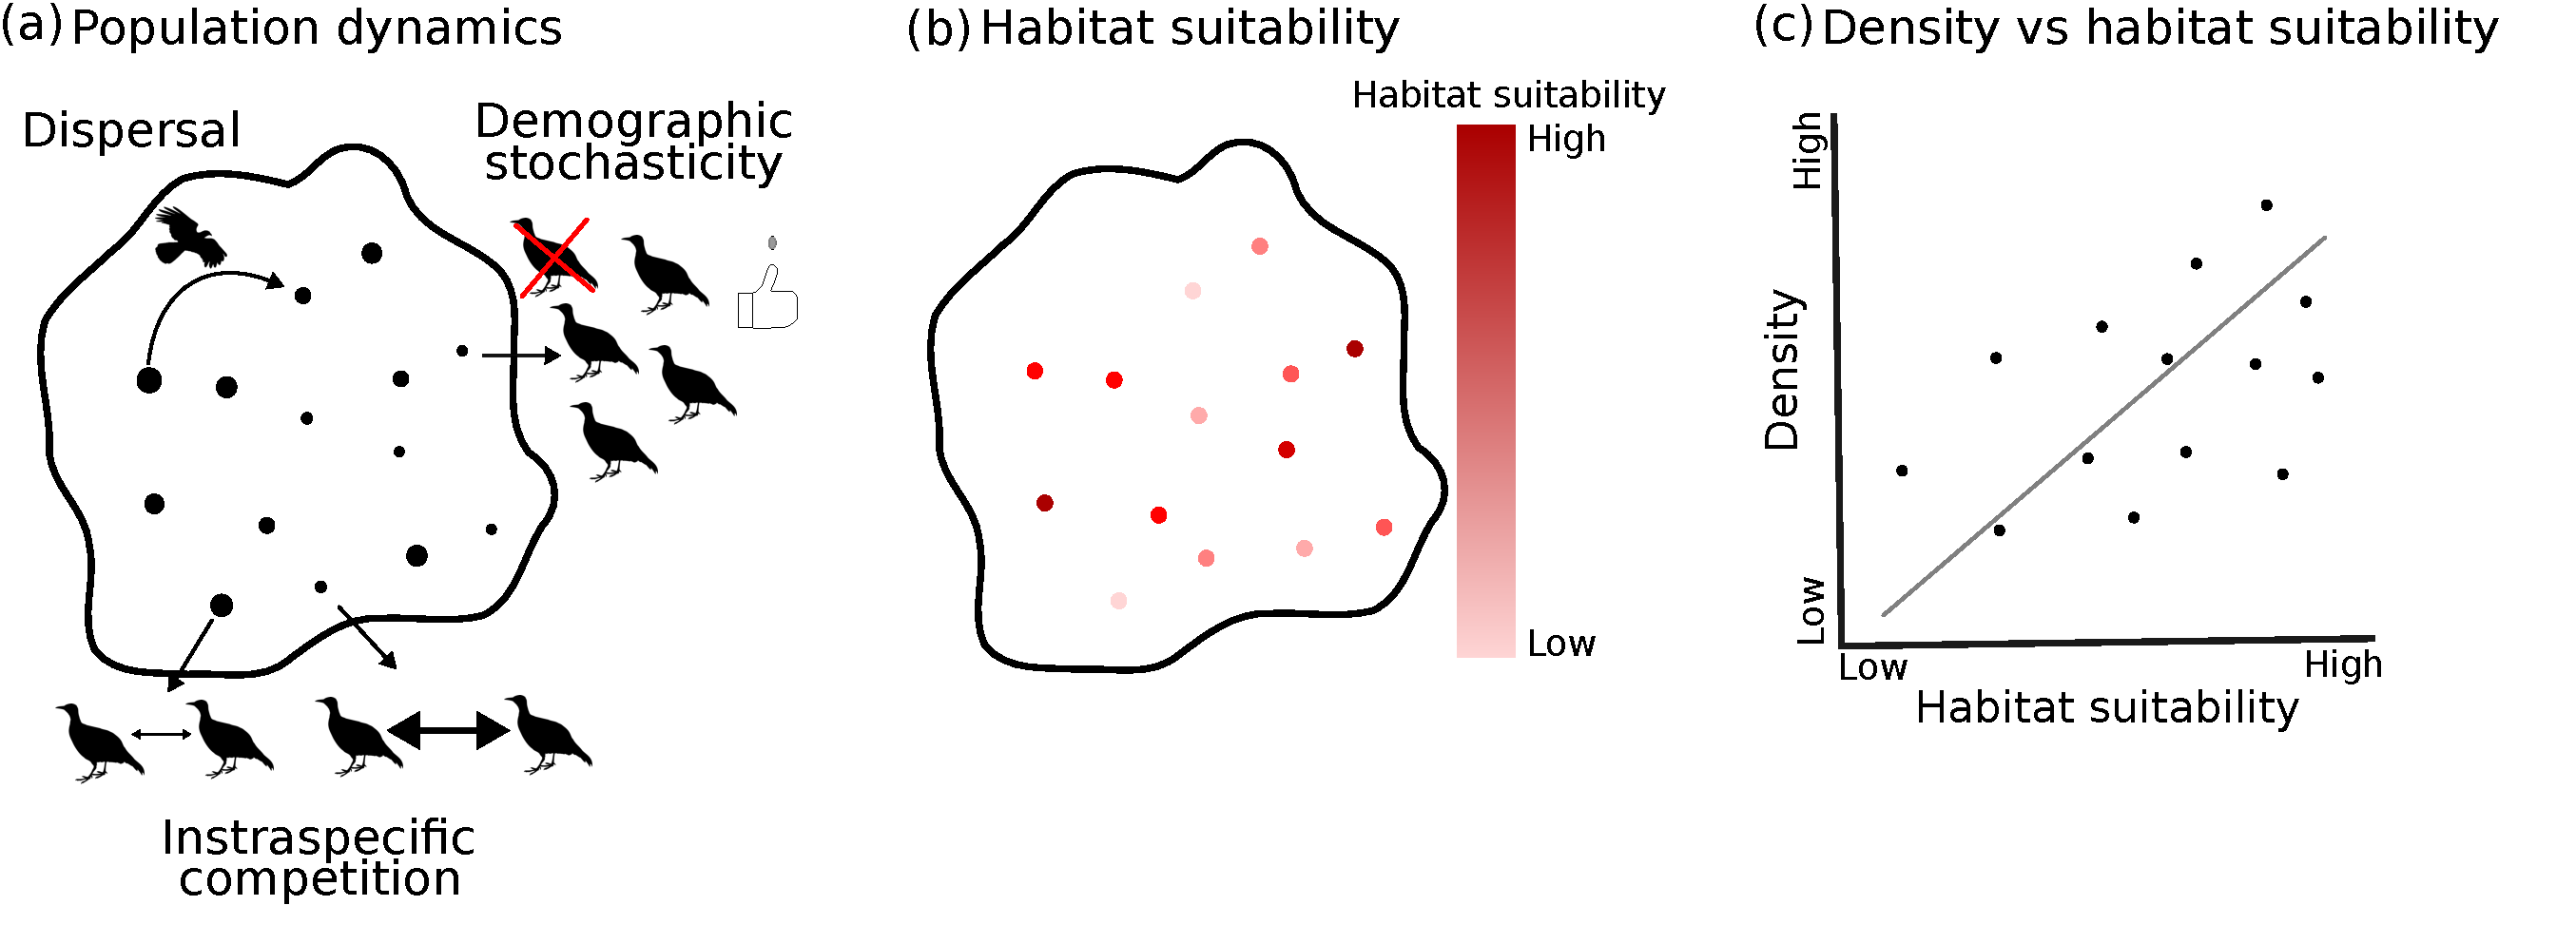
\includegraphics[width=1\textwidth]{FigsdmAbnd/Conceptual2}}
\caption[Simulating population dynamics]{Populations of virtual species were simulated considering dispersal dynamics, demographic stochasticity, spatial differences in intraspecific competition. Habitat suitability was estimated using species distribution models for sites were populations occurred (b) to explore the relationship (grey line) between habitat suitability and densities (c).} 
\label{fig:conce_sdmabnd}
\end{figure}
\clearpage

\begin{figure}[ht]
\centering
\centerline{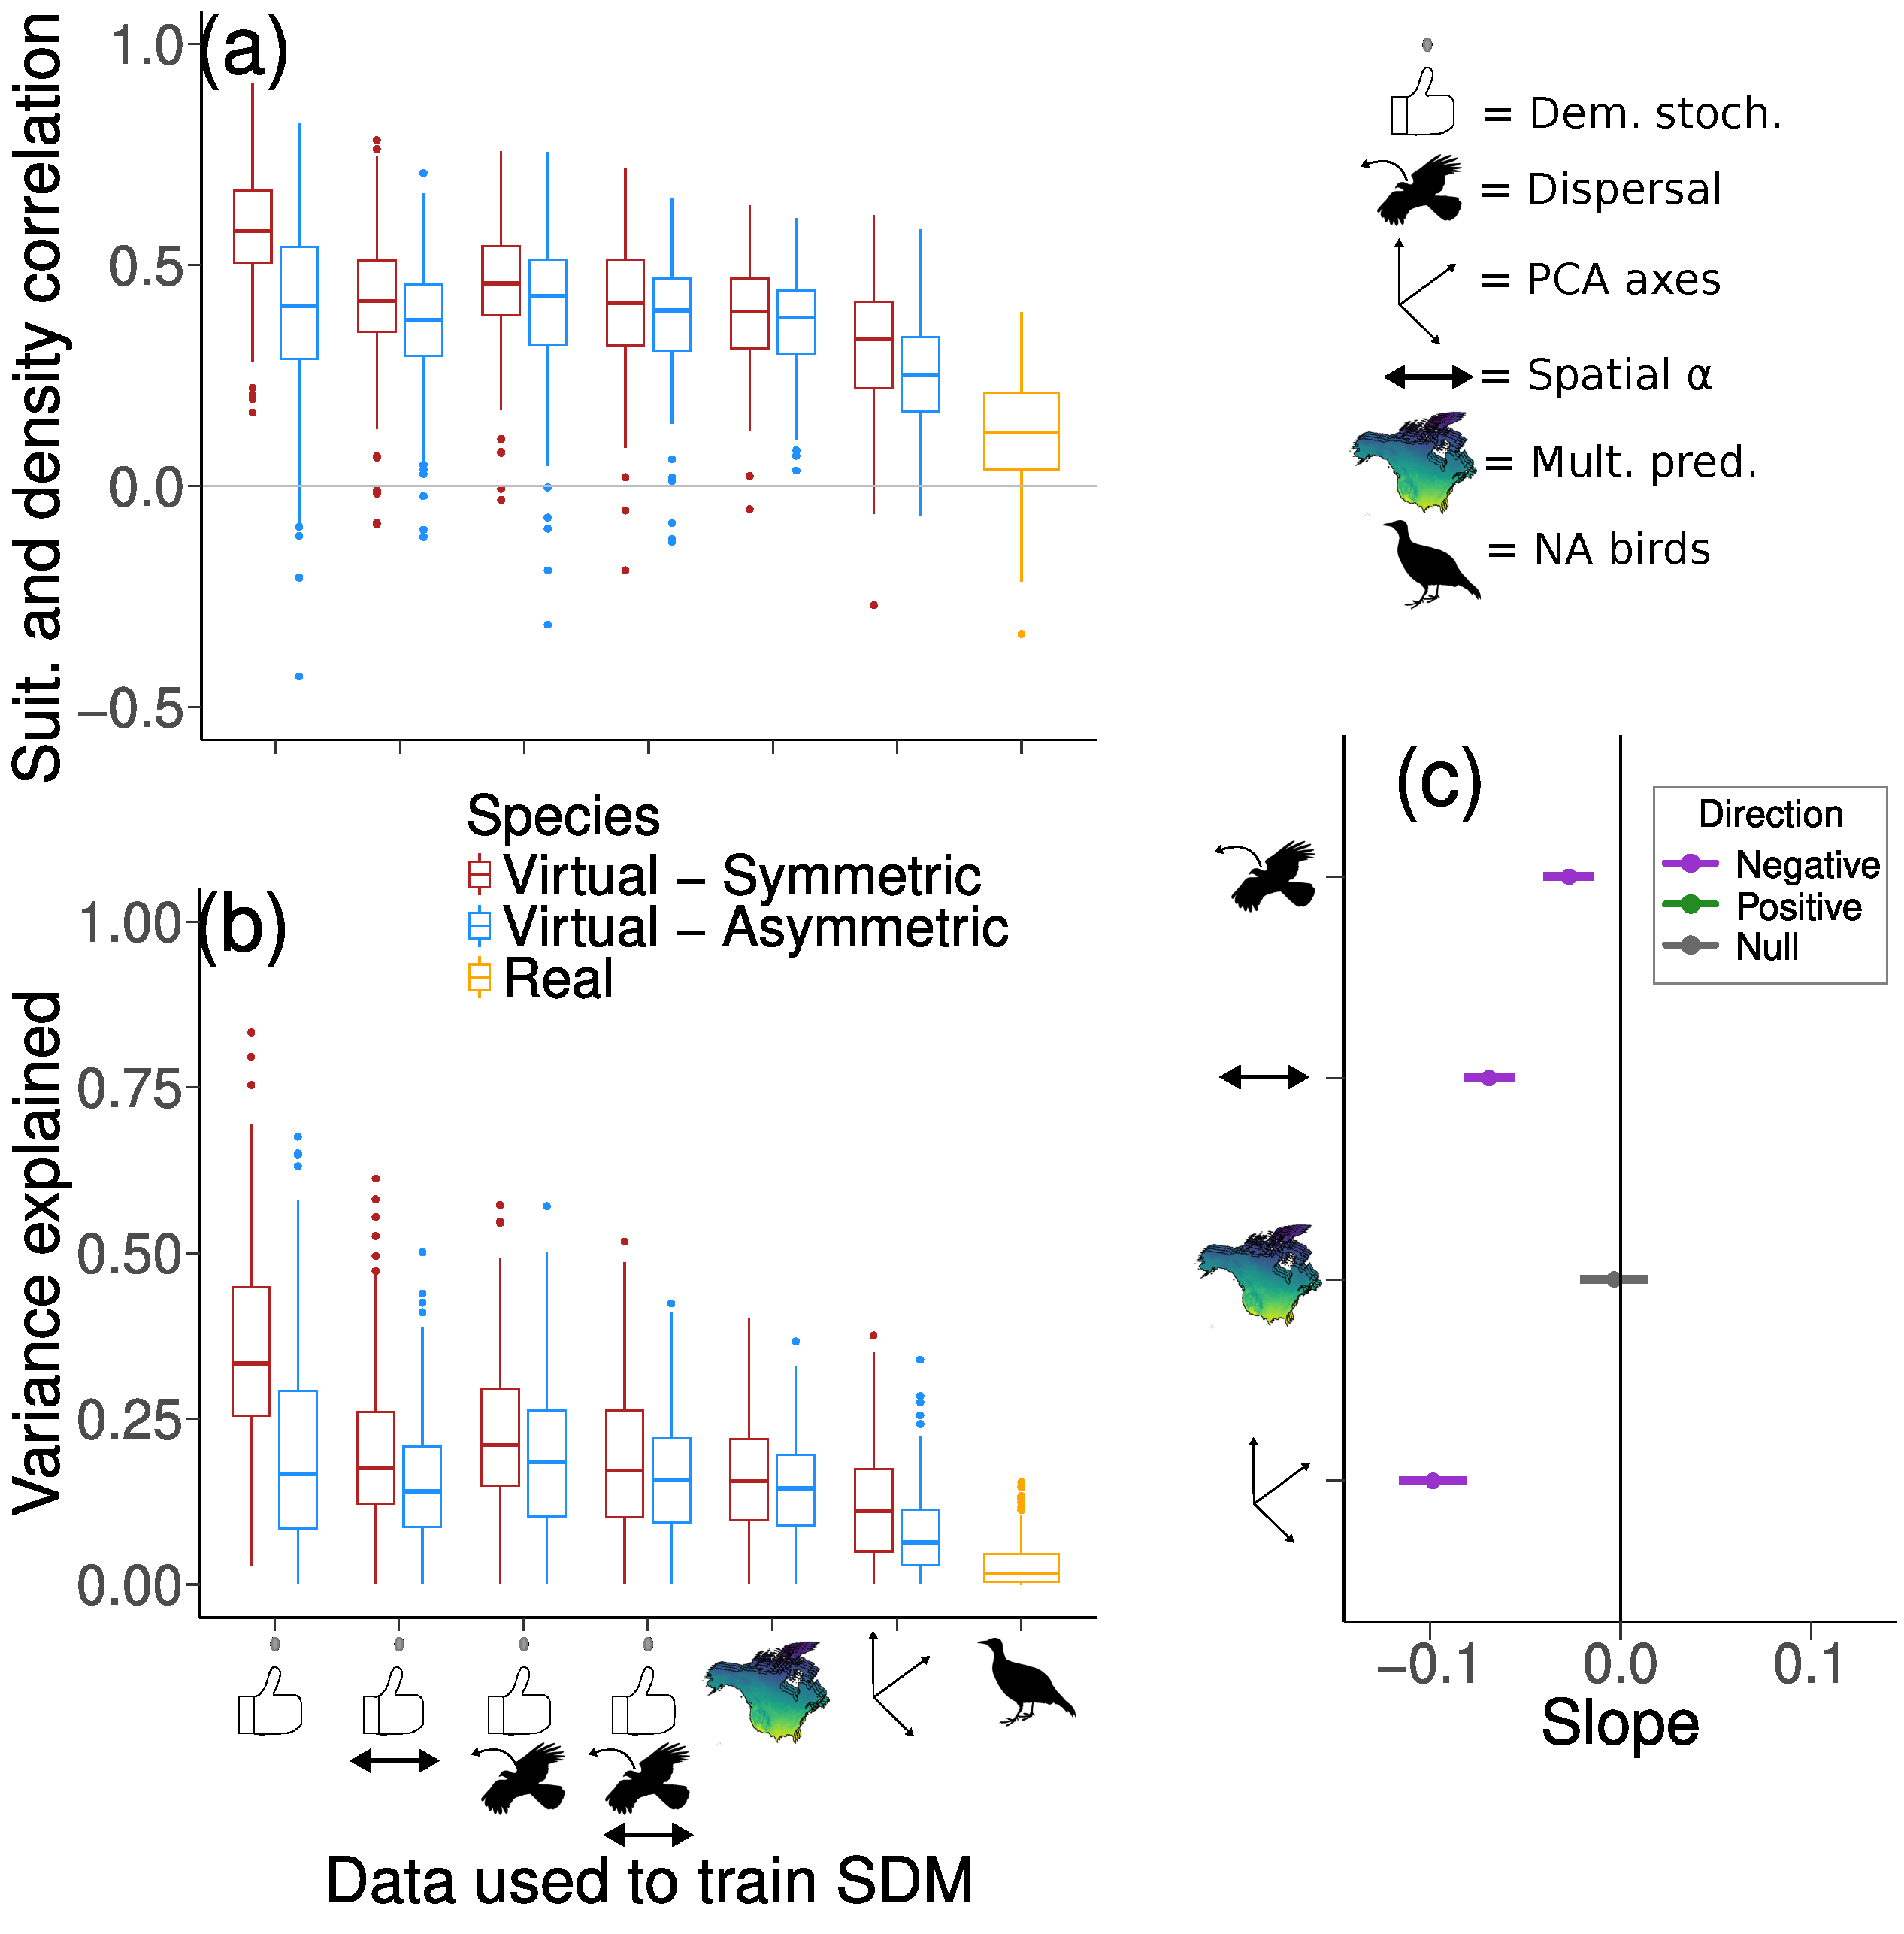
\includegraphics[width=1\textwidth]{FigsdmAbnd/Viores}}
\caption[Local factors influence how habitat suitability relates to density]{Observed correlations between habitat suitability and density for virtual species with symmetric and asymmetric performance curves and for North American birds.} 
\label{fig:cor}
\end{figure}
\clearpage


\begin{figure}[ht]
\centering
\centerline{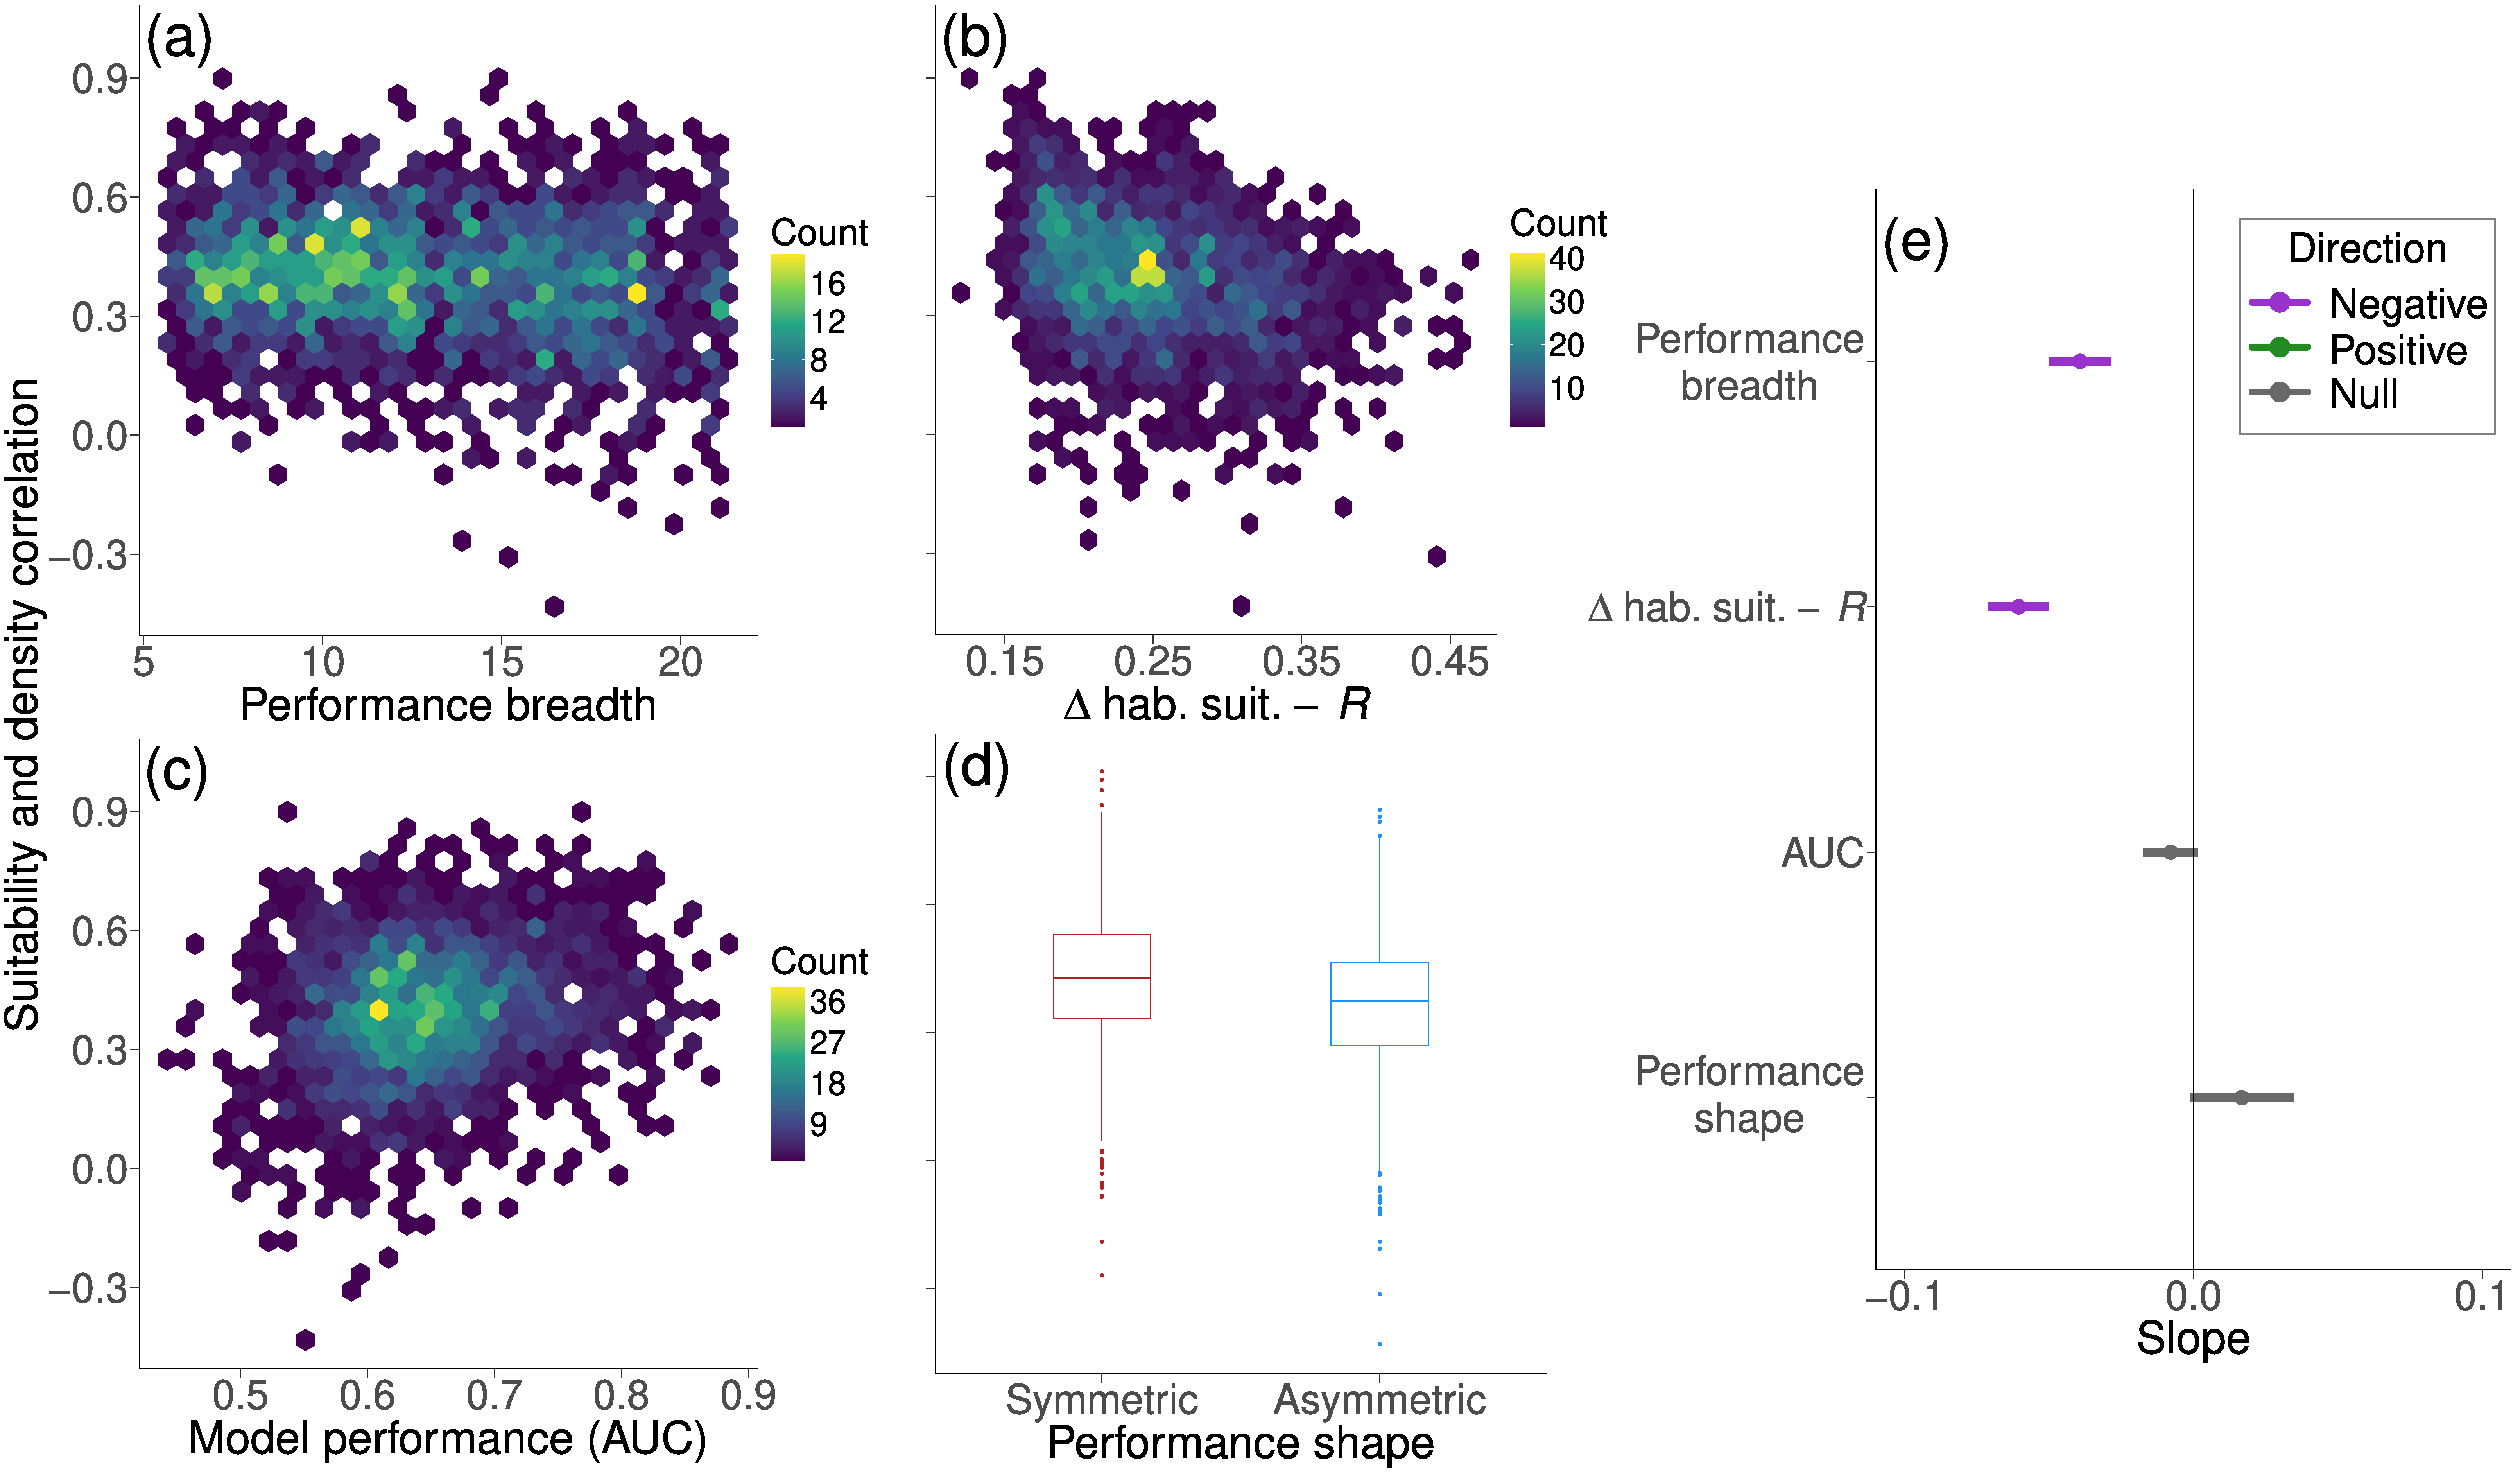
\includegraphics[width=1\textwidth]{FigsdmAbnd/RangeDiff}}
\caption[Species differences affect how habitat suitability relates to density]{The correlation between habitat suitability and density is affected by the species performance breadth, the ability of habitat suitability estimates to accurately represent population growth rates, but not by the average SDM performance and the shape of species performance curves.} 
\label{fig:diff}
\end{figure}



\addtocontents{toc}{\protect\vskip-20pt}
\chapter[Population variability across geographic ranges: Perspectives and challenges.]{Population variability across geographic ranges: Perspectives and challenges.\footnote[3]{Published as: Ten Caten, C., \& Dallas, T. (2025). Population variability across geographical ranges: perspectives and challenges. \textit{Proceedings B}, 292(2039), 20241644. Reproduced here under the CC BY 4.0 license terms. See Appendix D.}}    %% Calls Introduction.tex



\section*{\textbf{\underline{Abstract}}}
Populations fluctuate over time and across geographic space, and understanding how different factors contribute to population variability is a central goal in population ecology. There is a particular interest in identifying trends of population variability within geographic ranges as population densities of species can fluctuate substantially across geographic space. A common assumption is that populations vary more near species geographic range edges because of unsuitable environments and higher vulnerability to environmental variability in these areas. However, empirical data rarely supports this expectation, suggesting that population variability is not related to its position within species geographic ranges. We propose that performance curves, which describe the relationship between population growth rates and environmental conditions, can be used to disentangle geographic patterns of population variability. Performance curves are important for understanding population variability because populations fluctuate more in locations where they have lower growth rates due to unsuitable environmental conditions. This is important for the assessment of these geographic patterns in population variability because geographic edges often do not reflect environmental edges. Considering species performance curves when evaluating geographic patterns of population variability would also allow researchers to detect populations that are more susceptible to future changes in environmental conditions.\\

%-----------------------
\section*{\textbf{\underline{Introduction}}}
%\section*{Introduction}

A major goal in population ecology is to understand spatial and temporal patterns of population variability \parencite{arino1995,lundberg2000,williams2003}. Understanding population variability is important because more variable populations are at greater risk of going extinct due to the dramatic changes in peaks and crashes that such populations exhibit \parencite{lande1988, vucetich2000}. Considering population variability patterns has become an important component to aid conservation efforts \parencite{vucetich2000, burgess2020}, and there is a great interest in identifying the main drivers of population variability across different species. Population variability is affected by a myriad of intrinsic (e.g., demographic stochasticity and life-history traits) and extrinsic (e.g., fluctuactions in environmental conditions and patch quality) factors \parencite{lande1993, arino1995, melbourne2008}, where the importance of such factors in driving population variability likely varies across different populations.

A long-held hypothesis is that populations are more variable near the edges than near the center of species geographic ranges \parencite{gaston1990, lawton1993}. There is an expectation that sites occurring near range edges have poorer environmental conditions than sites occurring near the range center, making populations found near geographic range edges more vulnerable to environmental variability  \parencite{hardie2010,pironon2017}. This would decrease population growth rates, leading to smaller population sizes that are more variable due to demographic stochasticity being more prevalent in these populations (Figure \ref{fig:concept}). A reduced genetic diversity near geographic range edges could further contribute to an increase in population variability due to the lower adaptive potential of these populations \parencite{eckert2008, hardie2010}. Moreover, edge populations are often assumed to be more isolated, and less likely to receive immigrants through dispersal events, which could also affect the variability of these populations \parencite{burgess2020}. This could occur through meta-population dynamics, where edge populations are sometimes assumed to be sink populations that cannot exist without continued immigration from source populations \parencite{pulliam1988, furrer2016}. Despite these clear predictions that edge populations should be more variable than central populations, few studies have assessed these trends \parencite{sexton2009,pironon2017}. This likely stems from the challenging need of continuously sampling several populations across broad spatial extents to evaluate patterns of population variability within species geographic ranges, representing an important gap in our understanding of geographic patterns of population dynamics \parencite{curnutt1996, pironon2017}.

\begin{figure}[ht]
\centering
\centerline{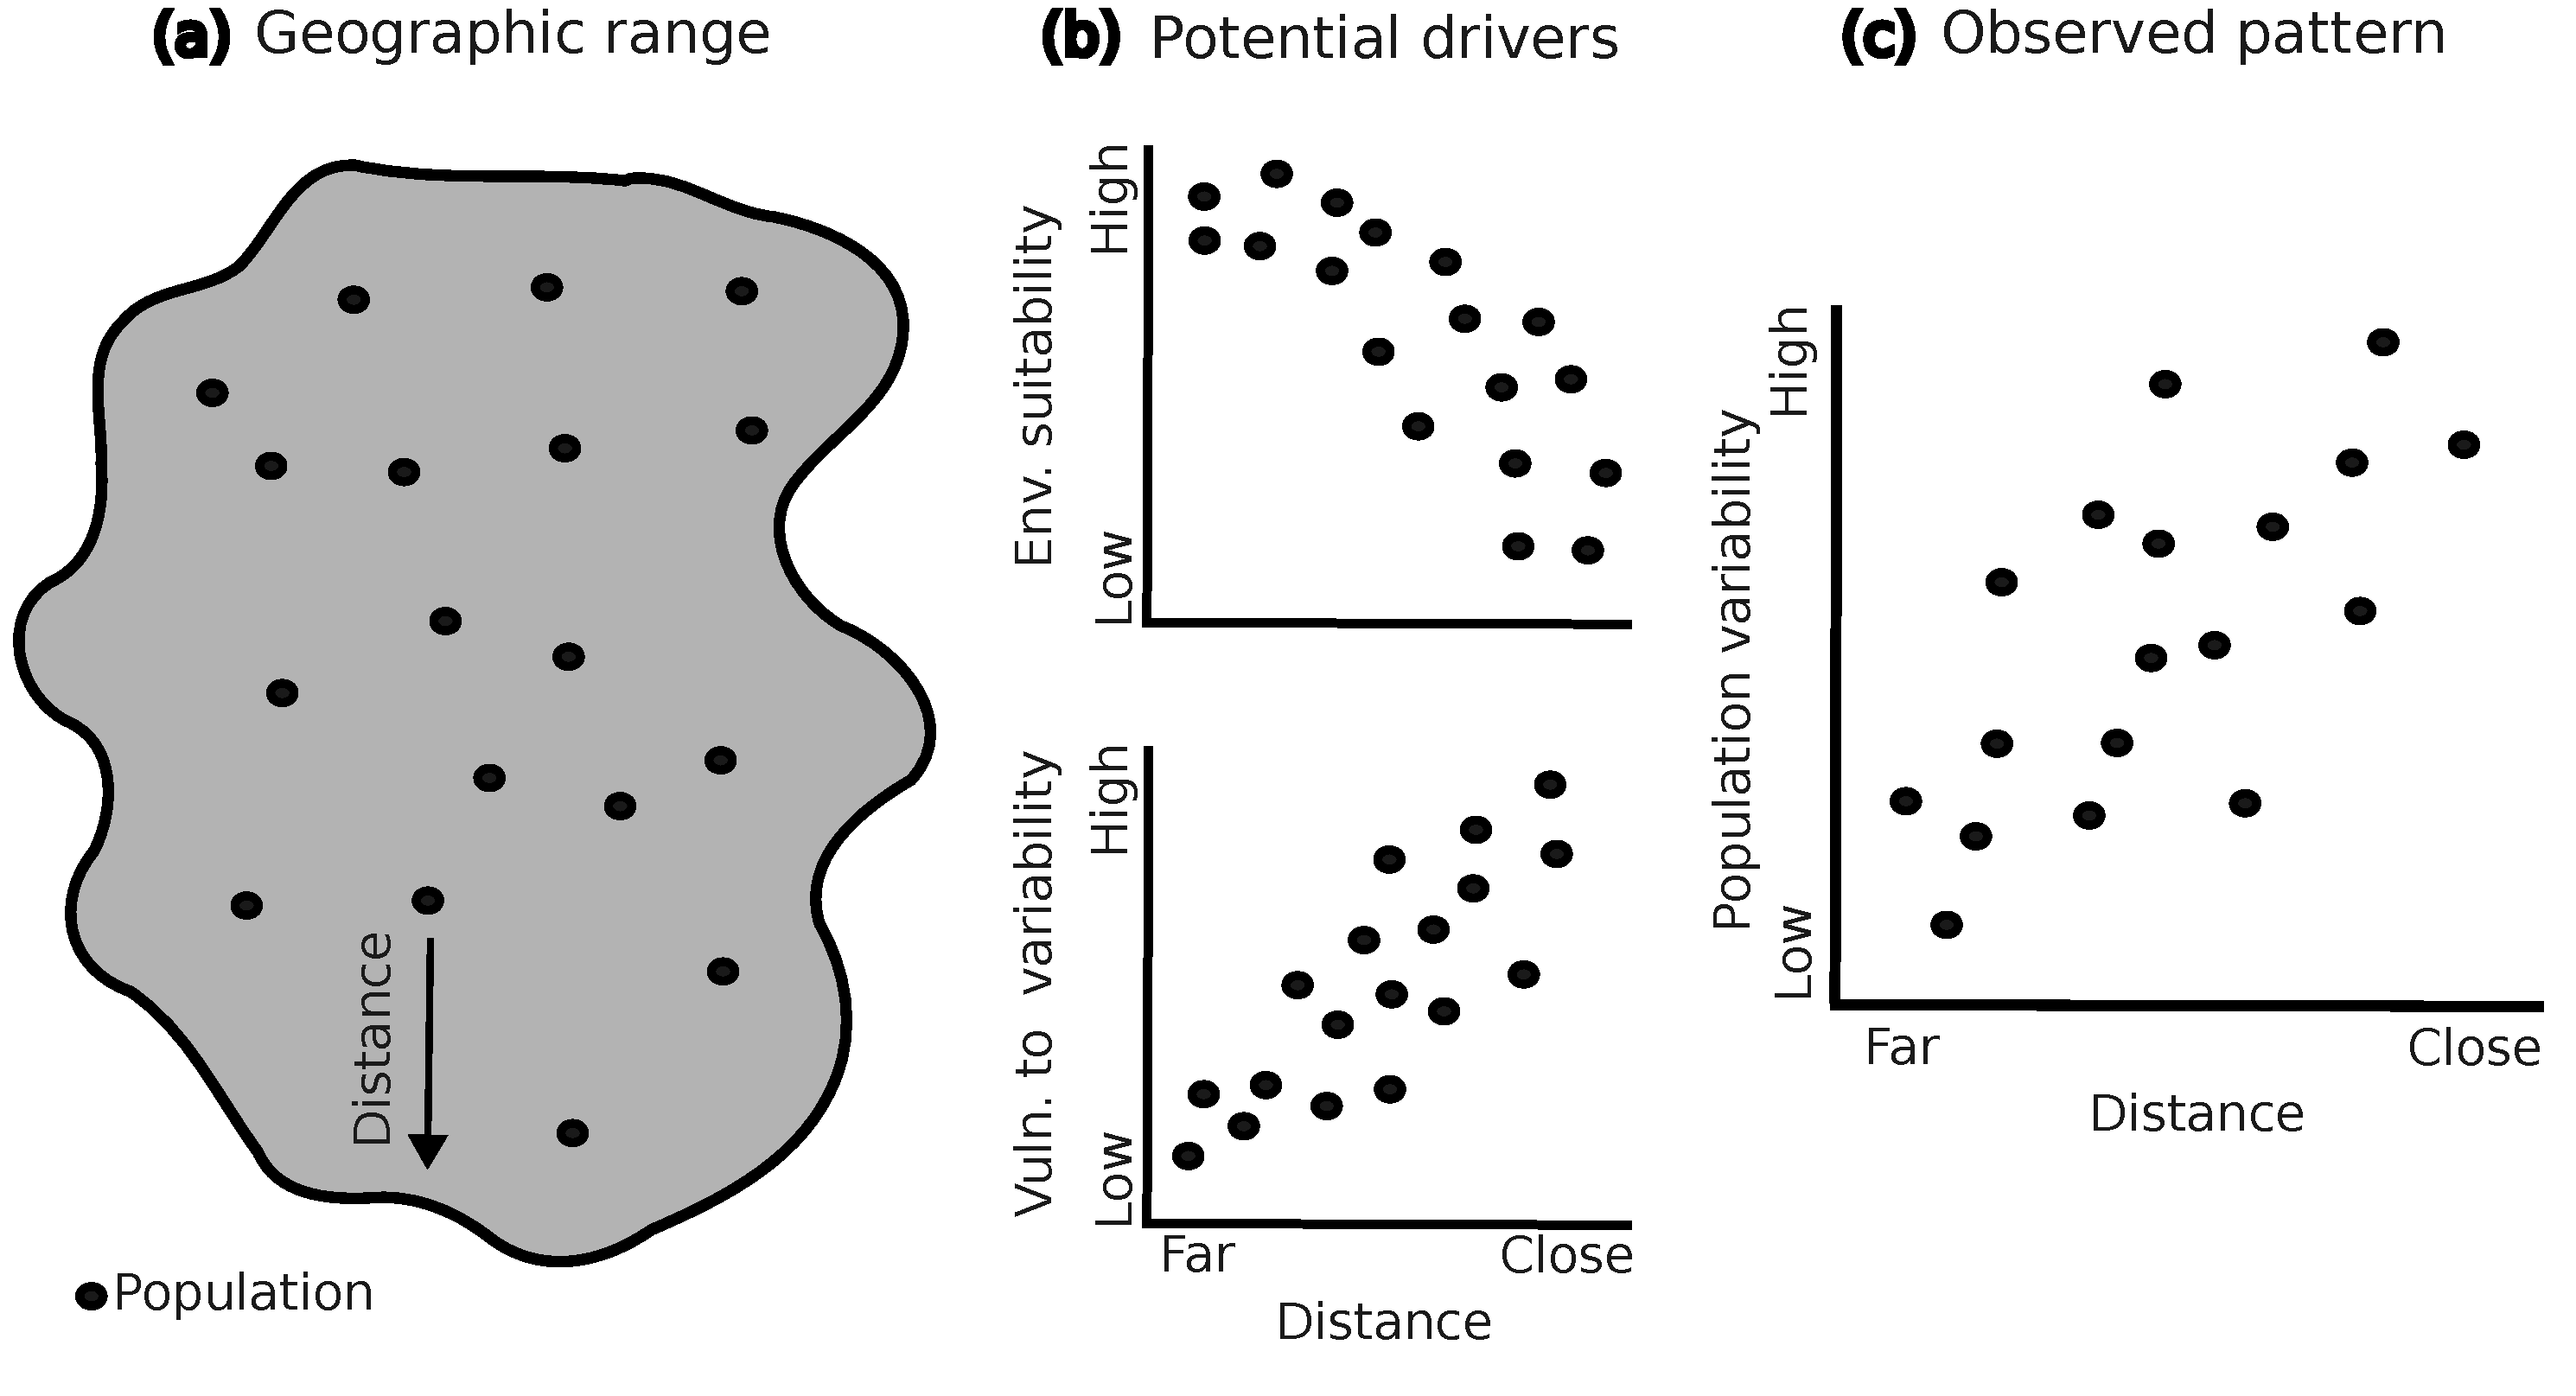
\includegraphics[width=1\textwidth]{FigRev/Conceptual}}
\caption[Population variability across geographic ranges]{Populations occurring closer to the edge of a species geographic range (a) are assumed to be exposed to less suitable and to be more vulnerable (Vuln.) to variable environmental (Env.) conditions (b) that would decrease growth rate and lead to more variable populations in those areas (c) due to smaller population densities and demographic stochasticity.} 
\label{fig:concept}
\end{figure}

Environmental conditions influence population dynamics such that vital rates and resulting population densities fluctuate more in variable than in constant environments \parencite{lundberg2000, tuljapurkar2009}. The effects of environmental conditions on population dynamics can be evaluated with performance curves, which describe the relationship between population growth rates and environmental conditions. Performance curves have been used to predict extinction risk, geographic range dynamics, and species responses to climate change \parencite{sinclair2016, huey2012, angilletta2009, buckley2008} while their use to examine differences in local population dynamics across geographic ranges remains unexplored. We propose that performance curves provide a valuable framework for understanding population variability across geographic ranges because populations fluctuate more in locations where they have lower growth rates due to unsuitable environments. Performance curves provide a direct link to how changing environmental conditions influence population growth rates and the population dynamics of a given species. This allows the simultaneous evaluation of how species-specific environmental responses and changing environmental conditions interact to shape geographic patterns of local population dynamics. This framework addresses a key assumption, that environmental conditions are poorer near range edges, that is often made when evaluating geographic patterns of population dynamics \parencite{sagarin2002,pironon2017}. Moreover, performance curves allow the identification of populations that are more susceptible to future climate change as environmental conditions will become unsuitable in parts of species geographic ranges \parencite{buckley2008, kingsolver2017}. 

We first provide a brief overview of some of the intrinsic and extrinsic factors that affect population variability and we synthesize the current evidence on population variability patterns across species geographic ranges. Intrinsic and extrinsic factors are defined as biological and non-biological components, respectively, that affect population growth rates and population dynamics. We use simulations to show that performance curves are useful to understand population variability and that having performance curves with different properties leads to contrasting geographic patterns of population variability across species. Lastly, important next steps in the study of spatial patterns in population variability are outlined. 
  
 
 
\subsection*{\textbf{\underline{Intrinsic drivers of population variability}}}
%\subsection*{Intrinsic drivers of population variability}
\paragraph*{Species traits}\mbox{}\\ 
Species traits are important factors that affect population dynamics. Body size is a key trait that influences population dynamics such that species that have small body sizes tend to have more variable populations than species with larger body sizes \parencite{lawton1986, gaston1988}. This occurs because species with small body sizes often have high population growth rates that can cause an increase in population variability through overcompensating density dependence when these species have nonoverlaping generations \parencite{may1974, gaston1988}. The dispersal ability of species could also impact population variability given that the dispersal of individuals between populations affect population variability \parencite{abbott2011}. Theoretical models predict that lower dispersal increases population variability, but experimental evidence supporting this expectation is limited \parencite{abbott2011, yang2022}. This indicates that different traits can potentially influence the patterns of population variability that species have. 


\paragraph*{Species interactions}\mbox{}\\ 
Species interactions can affect population dynamics because sites have limited resources that can be used by individuals of different species \parencite{macarthur1970, rhoades1985}. The type of interaction between two species can determine its effects on growth rates, such that mutualistic interactions have positive effects on population growth rates while antagonistic interactions negatively affect population growth rates \parencite{ehrlen1995, hale2021}. The strength of interactions, alongside the type of interaction, affects population dynamics such that strong interactions can lead to more or less variable populations depending on whether species are exhibiting mutualistic or antagostinic interactions \parencite{allesina2012,mougi2014}. However, changes in abiotic and biotic conditions along geographic space or over time can modify the effects of species interactions on population dynamics \parencite{travis1996, chamberlain2014}, suggesting that the level of interaction specialization \parencite{arino1995} and local environmental conditions can be important to determine population variability. 

  

\paragraph*{Demographic stochasticity}\mbox{}\\ 
Demographic stochasticity describes fluctuations in populations in a constant environment because of random events related to birth and death of individuals in a population \parencite{roughgarden1975, melbourne2008}. Some of the drivers of demographic stochasticity are stochastic sex determination and demographic heterogeneity. Stochastic sex determination leads to imbalances in the sex ratio of a population that often increases the variance of population growth rates whereas demographic heterogeneity relates to differences in birth and death probabilities of individuals of different sizes \parencite{saether2004b,melbourne2008}. The effects of demographic stochasticity are more prominent in small populations where it can often be the main driver of temporal variability in population densities \parencite{lande1993, melbourne2008}. Small populations usually have more variable growth rates \parencite{willi2009} and species with small population densities often have more variable populations than species with larger population densities \parencite{gaston1990, reed2004} likely because of demographic stochasticity.

%\subsection*{Extrinsic drivers of population variability}
\subsection*{\textbf{\underline{Extrinsic drivers of population variability}}}

\paragraph*{Environmental variability}\mbox{}\\ 
Fluctuations in environmental conditions are important extrinsic factors affecting population variability \parencite{bjornstad2001,melbourne2008}. Sources of environmental variability can be periodic, stochastic, and catastrophic. Periodic environmental variability are predictable changes in environmental conditions, such as seasonal differences in temperature \parencite{sabo2008}. Stochastic environmental variation occur through unpredictable sources of variability in the environment, and catastrophic sources of variability are rare extreme events, such as hurricanes, that significantly affects populations \parencite{sabo2008}. Here we use environmental variability to refer to stochastic environmental variations. More variable environments can increase population variability because of demographic constraints caused by extreme environmental conditions \parencite{bjornstad2001, boyce2006}. Variation in environmental conditions similarly affects all individuals in a population leading to decreases in long-term growth rates and more variable population dynamics \parencite{lewontin1969, melbourne2008, dee2020}. Environmental variability can have a stronger impact on population dynamics than changes in average environmental conditions \parencite{ruel1999,vasseur2014} but environmental variability can also increase long-term growth rate depending on the shape of the species performance curve \parencite{lawson2015}. This suggests that knowledge about species performance curves is essential to understand how environmental variability affects population dynamics.



\paragraph*{The geography of occupied patches}\mbox{}\\ 
The spatial structure of patches where populations occur affects population density \parencite{munguia2014}. Small and isolated patches often have smaller and more variable populations than larger and well-connected patches \parencite{taylor1990}. Small patches have smaller populations because of the limited space and resources available for species in these locations that reduce population growth rates \parencite{connor2000, hokit2003, londono2007}. This can amplify the effects of demographic stochasticity in populations found in these areas. Individuals are less likely to migrate to highly isolated patches, such that this decrease in dispersal is often linked to more variable population dynamics \parencite{hanski1998, abbott2011}. Thus, an interplay between patch area and isolation can lead to differences in population dynamics across geographic ranges.


\paragraph*{The possible interaction between different drivers of population variability}%\mbox{}\\ 

Population variability might be driven through an interplay between intrinsic and extrinsic factors. For example, both demographic stochasticity and fluctuating environmental conditions can similarly drive population dynamics depending on the size of the populations \parencite{melbourne2008}. Increasing levels of environmental variability lead to contrasting population dynamics between interacting species when they respond differently to environmental conditions  \parencite{dee2020}, further exemplifying the interaction between different mechanisms driving population variability. This highlights that the assessment of population variability patterns across geographic space can be a complex task as multiple mechanisms might interact to drive such dynamics.
 



%A lof of these factors interact with each other (e.g., Ives et al. 2004)
%\subsection*{Gauging support for geographic patterns of population variability}
\section*{\textbf{\underline{Gauging support for geographic patterns of population variability}}}

We conducted literature searches on Web of Science (WoS) to obtain articles that evaluated population variability patterns across species geographic ranges. We performed our search using individual keywords combined with boolean operators (restricting or expanding the search using "OR" and "AND"), and asterisk to consider multiple words that have different endings. Our search was performed on February 6 2024, using the following search terms: "population varia*" OR "population stability" AND "geographic range" OR "range position". We restricted our search to the field Ecology, resulting in 1302 articles. We filtered this initial list to keep articles that compared temporal trends of population variability across different parts of species geographic ranges by screening articles title and abstract. Studies that compared trends of population variability across species or at the community level were not considered. This resulted in a final pool of five studies from our WoS search. We checked the references and articles that cited these five studies to include studies that were not returned in our search, resulting in four additional studies being added to our list (Table \ref{tab:List}). 


Despite being considered "conventional wisdom" \parencite{vucetich2003}, we found that the relationship between population variability and geographic range position has been severely under-assessed compared to geographic trends in population density or genetic variability \parencite{sexton2009,pironon2017}. We observed taxonomic biases in the studies we found, where population variability was often evaluated for animal species, and we did not find studies considering plant species. This lack of studies using plant species likely stems from the fact that most assessments of variability in plant population dynamics consider the variability of demographic parameters (e.g., recruitment and survival) across species geographic ranges \parencite{villellas2013, pironon2018} rather than variability in population densities. As demographic parameters might vary in different directions across plant species geographic ranges (i.e., demographic compensation \parencite{doak2010,villellas2015, pironon2018}), and it is unclear how these contrasting geographic trends of variability in these demographic parameters would affect spatial patterns of population variability, we did not consider these studies. We acknowledge that some studies have evaluated the variation of population growth rates across geographic ranges of plant species \parencite{volis2004,kluth2005,angert2009}, which could be used as a proxy for population variability. We did not consider these studies in our analyses because these population growth rates were often estimated through matrix models that make assumptions, such as equal survival and fecundity of adults derived from seeds of different ages, that are challenging to consider in our assessment.


The majority of the studies evaluating patterns of population variability considered terrestrial species and occurred in the Northern Hemisphere (Table \ref{tab:List}). The most often used estimates of population variability were the coefficient of variation (CV) and the standard deviation (SD) of population densities. Alternatively, there were different estimates that were used to represent the position of populations within species geographic ranges. Latitude was the most commonly used estimate of geographic range position  \parencite{hansson1985,forchhammer1993, thomas1994, saether2008}. Using latitude as a proxy for position within the species geographic range might be inadequate because populations should be more variable near geographic range edges regardless of latitude. Two populations that are found at the same latitude within the species geographic range could have different geographic range position, because they are found at different longitudes, and would supposedly exhibit contrasting patterns of population variability. However, considering latitude as a proxy for geographic range position is understandable given that several environmental conditions that are thought to be major drivers of population variability might exhibit a latitudinal gradient \parencite{hansson1985}. Other estimates of range position included distance to geographic range edge \parencite{curnutt1996}, geographic scoring \parencite{saitoh1998}, site northing \parencite{oliver2012}, elevation \parencite{fukaya2014}, and population density \parencite{williams2003}. 

\begin{table}[ht]
\centering
\caption[Studies that assessed geographic patterns of population variability]{List of articles that evaluated the occurrence of patterns of population variability across species geographic ranges.} 
\resizebox{\textwidth}{!}{\begin{tabular}{cccccc}
  \hline
Variability estimate & Predictor & Species (\textit{n}) &Sig. (\textit{n}) and dir. & Region &Reference \\ \hline
 CV & Latitude (cont.) & 24 & 6(+) &Great Britain & Thomas et al. 1994 \parencite{thomas1994}\\ 
 SD & --- & --- & 7(+) & --- & --- \\ 
 \textit{log} CV & Distance to edge (cont.)& 6 & 2 (+) & North America & Curnutt et al. 1996
 \parencite{curnutt1996} \\ 
 SD[\textit{log$_{10}$}(\textit{n})] & Geographic score (cont.)& 1 & 1(+) & Japan &Saitoh et al. 1998 \parencite{saitoh1998} \\
 amplitude & ---  & ---  & ---  & ---  & --- \\ 
 CV & Density (cont.) & 3 & 3(+) & North America & Williams et al. 2003 \parencite{williams2003} \\ 
 CV & Site northing (cont.) & 19 & 4(+) & Great Britain & Oliver et al. 2012 \parencite{oliver2012} \\ 
 SD[\textit{log}(\textit{n})] & ---  & ---  &  2(+) & ---  & ---  \\ 
 SD[\textit{log}(\textit{n})] & Elevation (disc.) & 1 & 1 (+)\ & Japan & Fukaya et al. 2014 \parencite{fukaya2014}\\ 
 var[\textit{log}(\textit{n})] & Latitude (cont.) & 8 & 5 (-) & North America & Saether et al. 2008 \parencite{saether2008} \\ 
 CV & Latitude (cont.) &2 & 2 (+) & Fennoscandia& Hansson \& Henttonen 1985 \parencite{hansson1985} \\ 
 \textit{s} & ---  & ---  & ---  & ---  & ---  \\ 
 SD[residuals]  & Latitude (cont.) &1 & 0 &North America &Forchhammer \& Boertmann 1993 \parencite{forchhammer1993} \\ 
   \hline
\end{tabular}}
\label{tab:List}
\end{table}


Overall, the four studies that found support for the occurrence of more variable populations near geographic range edges considered fewer than five species \parencite{hansson1985,saitoh1998, williams2003, fukaya2014}, although a lack of relationship between range position and population variability was also reported in a study that considered one species \parencite{forchhammer1993}. Conversely, three studies that considered over five species often found support for the occurrence of more variable populations near geographic range edges for only approximately 30\% of the species considered \parencite{thomas1994, curnutt1996, oliver2012}, and in one study opposite patterns (i.e., less variable populations near range edges) were observed \parencite{saether2008}. This prevalence of 30\% of the species exhibiting geographic patterns of population variability is similar to the observed prevalence of geographic patterns of population density \parencite{sagarin2002, pironon2017}, suggesting that trends of population density and population variability within geographic ranges are not common. Nonetheless, it still remains an open question whether the same species show similar patterns of population density and population variability across geographic ranges given that these trends are often evaluated separately from each other, and there is an expectation that similar mechanisms drive population variability and density across geographic ranges \parencite{sagarin2002}.

Our search shows that most of the support for the expectation that species have more variable populations near their geographic range edges comes from studies that evaluated these patterns for small sets of species, while there is a lack of studies evaluating these relationships for larger sets of species, representing an important knowledge gap in our understanding of population dynamics across species geographic ranges. The data needed to evaluate these trends of population variability across geographic ranges need to cover a broad spatial and temporal scale, being a clear limiting factor when addressing these questions. These challenges can be overcome through the use of large-scale monitoring programs that continuously record species occurrence and abundance at different locations (e.g., Breeding Bird Survey and the United Kingdom Butterfly Monitoring Scheme), community-maintained databases that summarizes collection of assemblage data worldwide (e.g., BioTIME and sPlotOpen) or through the use of citizen-science databases (e.g., eBird and iNaturalist). However, spatial biases in sampling and in over-representation of species with specific traits may need to be addressed before using citizen-science databases to answer questions on population dynamics across species geographic ranges \parencite{bird2014,callaghan2021}.


\section*{\textbf{\uline{Why are patterns of population variability across geographic ranges rarely observed?}}}
%\section*{\textbf{\underline{Why are patterns of population variability across geographic ranges rarely \mbox{observed?}}}}

Patterns in population variability across species geographic ranges have not been widely evaluated, and we found limited evidence supporting the occurrence of such trends. This lack of support for this expectation could be explained by different factors. For example, it is assumed that species are in equilibrium and that environmental conditions gradually deteriorate towards the edges of species geographic ranges, ultimately leading to more variable population dynamics in these regions. While several environmental conditions exhibit latitudinal gradients \parencite{frenne2013} it is unclear why environmental conditions would gradually become unsuitable towards all edges of species geographic ranges. Variables affecting population dynamics could operate at a finer spatial scale than studies often consider and have low spatial structure \parencite{lawton1993,pironon2017}. This can cause heterogeneity in landscapes and influence the spatial signal in how population variability is structured across geographic space. For example, landscape heterogeneity caused by topographic variability can provide suitable microclimatic conditions near edges of geographic ranges that can reduce population variability in these locations \parencite{oliver2010,carnicer2021}.


Populations occurring in different parts of species geographic ranges can have different types of adaptations to local environmental conditions that stabilize population dynamics across their geographic ranges \parencite{oldfather2018}. For example, populations of plant species occurring across gradients of aridity might show specific local adaptations in morphological leaf traits that improve their performance when occurring in unfavorable conditions \parencite{ramirez2014, carvajal2017}. These adaptations to different environmental conditions across geographic ranges can involve several traits that are associated with different aspects of population performance \parencite{emery2017, latron2023}. This can lead to the occurrence of demographic compensation across geographic ranges (e.g., a higher death rate in a given location can be offset by increased fecundity of that population) and lead to similar patterns of population variability across geographic ranges \parencite{doak2010, villellas2015}. Although not all species show demographic compensation \parencite{pironon2018,sheth2018,oldfather2021}, demographic compensation could explain the lack of population variability patterns across geographic ranges of most species.
 

Populations can be more or less variable depending on their position within the species thermal performance curve and the amount of environmental variability that they experience \parencite{lawson2015, evans2022}. For example, populations found in warmer locations are more susceptible to temperature fluctuations independent of their position within the species geographic range \parencite{beaty2023,lewis2023}. This indicates that position of a population within the species thermal performance curve might be a more important predictor of population variability than geographic range position. Populations can also exhibit local adaptations in their thermal performances such that populations found in warmer environments can be more tolerant to warming conditions \parencite{herrando2019} and populations found in the colder environments could be more tolerant to lower temperatures \parencite{chiba2016}. Although species performance curves are often described in terms of thermal performance along temperature gradients, other environmental conditions might be more important to determine population dynamics of a given species \parencite{chambers2018}. This suggests that environmental conditions and the position of a population within the species performance curve, and not geographic range position, are key factors driving population variability across geographic ranges. 


%\subsection*{The importance of the shape of species performance curves}
\section*{\textbf{\underline{The importance of the shape of species performance curves}}}

Population dynamics could be better understood based on the position of populations within species niches rather than based on their position within geographic ranges \parencite{yanez2012,martinez2013}. This links how species niche requirements affect their geographic distribution \parencite{pulliam2000} and addresses some of the issues with using geographic range position as predictor of population dynamics. However, the niche describes the set of environmental conditions needed for a species to persist indefinitely in an area \parencite{hutchinson1957}, suggesting that using the niche to evaluate population dynamics might be challenging. For example, a species may have a niche that allows it to persist in locations that have temperatures between 8$^{\circ}$C and 30$^{\circ}$C. Determining how this species population dynamics change along this temperature gradient based on the niche is difficult as the relationship between population growth rate and temperature can have different shapes that would lead to contrasting patterns of population dynamics along this temperature gradient.
 
Performance curves have been used to understand the effects of environmental conditions on population growth rates and how that affects extinction risks and limits species geographic distributions \parencite{buckley2008, angilletta2009}. Spatial differences in environmental conditions affect population dynamics such that performance curves can be also used to elucidate patterns of population variability that are observed within the geographic ranges of different species. We show that differences in the shape (i.e., the level of symmetry)  that species exhibit in their performance curves \parencite{buckley2022} is sufficient to lead to contrasting patterns of population variability across their geographic ranges even when their performance curves have the same optimum (see Box 1). This occurs because some environmental conditions have different effects on the population dynamics of species with performance curves of different shapes. These results show that performance curves are important determinants of species differences in patterns of population variability across geographic ranges in addition to limiting population growth rates and geographic distributions \parencite{buckley2008, angilletta2009}. Considering species performance curves allows a disentanglement of geographic population variability trends according to the environmental conditions that populations are being exposed to in a given area. This is an important step towards understanding spatial patterns of population variability as geographic and climatic edges are not concordant for most species \parencite{oldfather2019,pennington2021}. 
 

\begin{tcolorbox}[breakable, enhanced, colback = white, title={Box 1}]

Species performance curves often describe the relationship between population growth rate and environmental conditions. Considering the shape of performance curve can be crucial to understanding patterns of population variability within species geographic ranges. Species performance curves can have different shapes (e.g., symmetric and asymmetric \parencite{buckley2022}) that can be enough to affect patterns of population variability within species geographic ranges, and might explain why species exhibit different geographic patterns of population variability. 

To demonstrate the influence of the shape of the performance curve on geographic patterns of population variability, we simulated the population dynamics of two species that have performance curves with different shapes across the same landscape. We used North America as landscape (7403 cells), and we considered mean annual temperature, ranging from $\approx -8$ $^{\circ}$C to $\approx 27$ $^{\circ}$C , as the environmental condition that affected our virtual species (Figure \ref{fig:spatvar}a). The population dynamics of both species were modeled following a discrete time Ricker model, where populations grow according to rate \textit{R} and intraspecific competition ($\alpha$ = 0.005) limits population size \textit{N}. The number of offspring obtained in each generation is estimated from a Poisson distribution with mean \textit{R}, and survivorship at each time step is defined by a binomial random variable with probability $e^{- \alpha N_{t}}$. These two processes represent the main drivers of demographic stochasticity in this model. Note that in this model there is no dispersal occurring between the different populations. 

\begin{equation}
\label{eq:ricker}
N_{t+1} = N_{t} \ R \ e^{- \alpha N_{t}}
\end{equation}  

The \textit{R} of a population in a given location was estimated based on the performance curve of each species. The main difference between the species performance curves is their shape, where one species has a symmetric and the other has an asymmetric performance (Figure \ref{fig:spatvar}d-e). Both species have the same optimum environmental condition (13$^{\circ}$C), and the area under the curve for which populations are able to persist indefinitely (i.e., \textit{R}>=1) is also the same for both species. This illustrates a case where species achieve their highest performance under similar environmental conditions, but that their performance deteriorates at a different rate away from this optimum.

We started the simulation with every cell in the landscape being occupied by 50 individuals, and we ran the models for 200 generations. We calculated the coefficient of variation in abundance to estimate population variability for all cells that did not go extinct between generations 100-200. We assessed the relationship between population variability and distance to the geographic range edge using Spearman's correlation to account for potential non-linearities in these relationships. The species with an asymmetric performance curve occupied $\approx$ 11\% more cells than the species with a symmetric curve, and it also had, on average, slightly less variable populations across the landscape (Figure \ref{fig:spatvar}b-c). The relationship between variability and distance to geographic range edge was influenced by the shape of the performance curves. The species with a symmetric performance curve tended to have more variable populations near range edges ($\rho$ = -0.38, p < 0.01; Figure \ref{fig:spatvar}f) while this relationship was much weaker for the species with an asymmetric performance curve ($\rho$ = -0.07, p < 0.01; Figure \ref{fig:spatvar}g). This highlights that differences in the shape of species performance curves affect geographic patterns of population variability even when species achieve their highest performance under similar environmental conditions.

The occurrence of dispersal events between populations can strongly influence observed geographic patterns of population variability. In our simulation, population variability was only estimated for sites where the species had a \textit{R}$\ge$1. This was done to isolate the effects of the shape of species performance curve on population variability across geographic space, but it is a simplified representation of population dynamics. By allowing dispersal of individuals between sites, the occurrence of source-sink dynamics becomes possible, where populations that are sinks (i.e., they have \textit{R} < 1) can be maintained through continuous dispersal from source populations. This continuous dispersal of individuals between source and sink sites could have direct impacts on trends of population variability as dispersal can increase or decrease population variability \parencite{abbott2011, yang2022}.
\clearpage 
{
\begin{center}
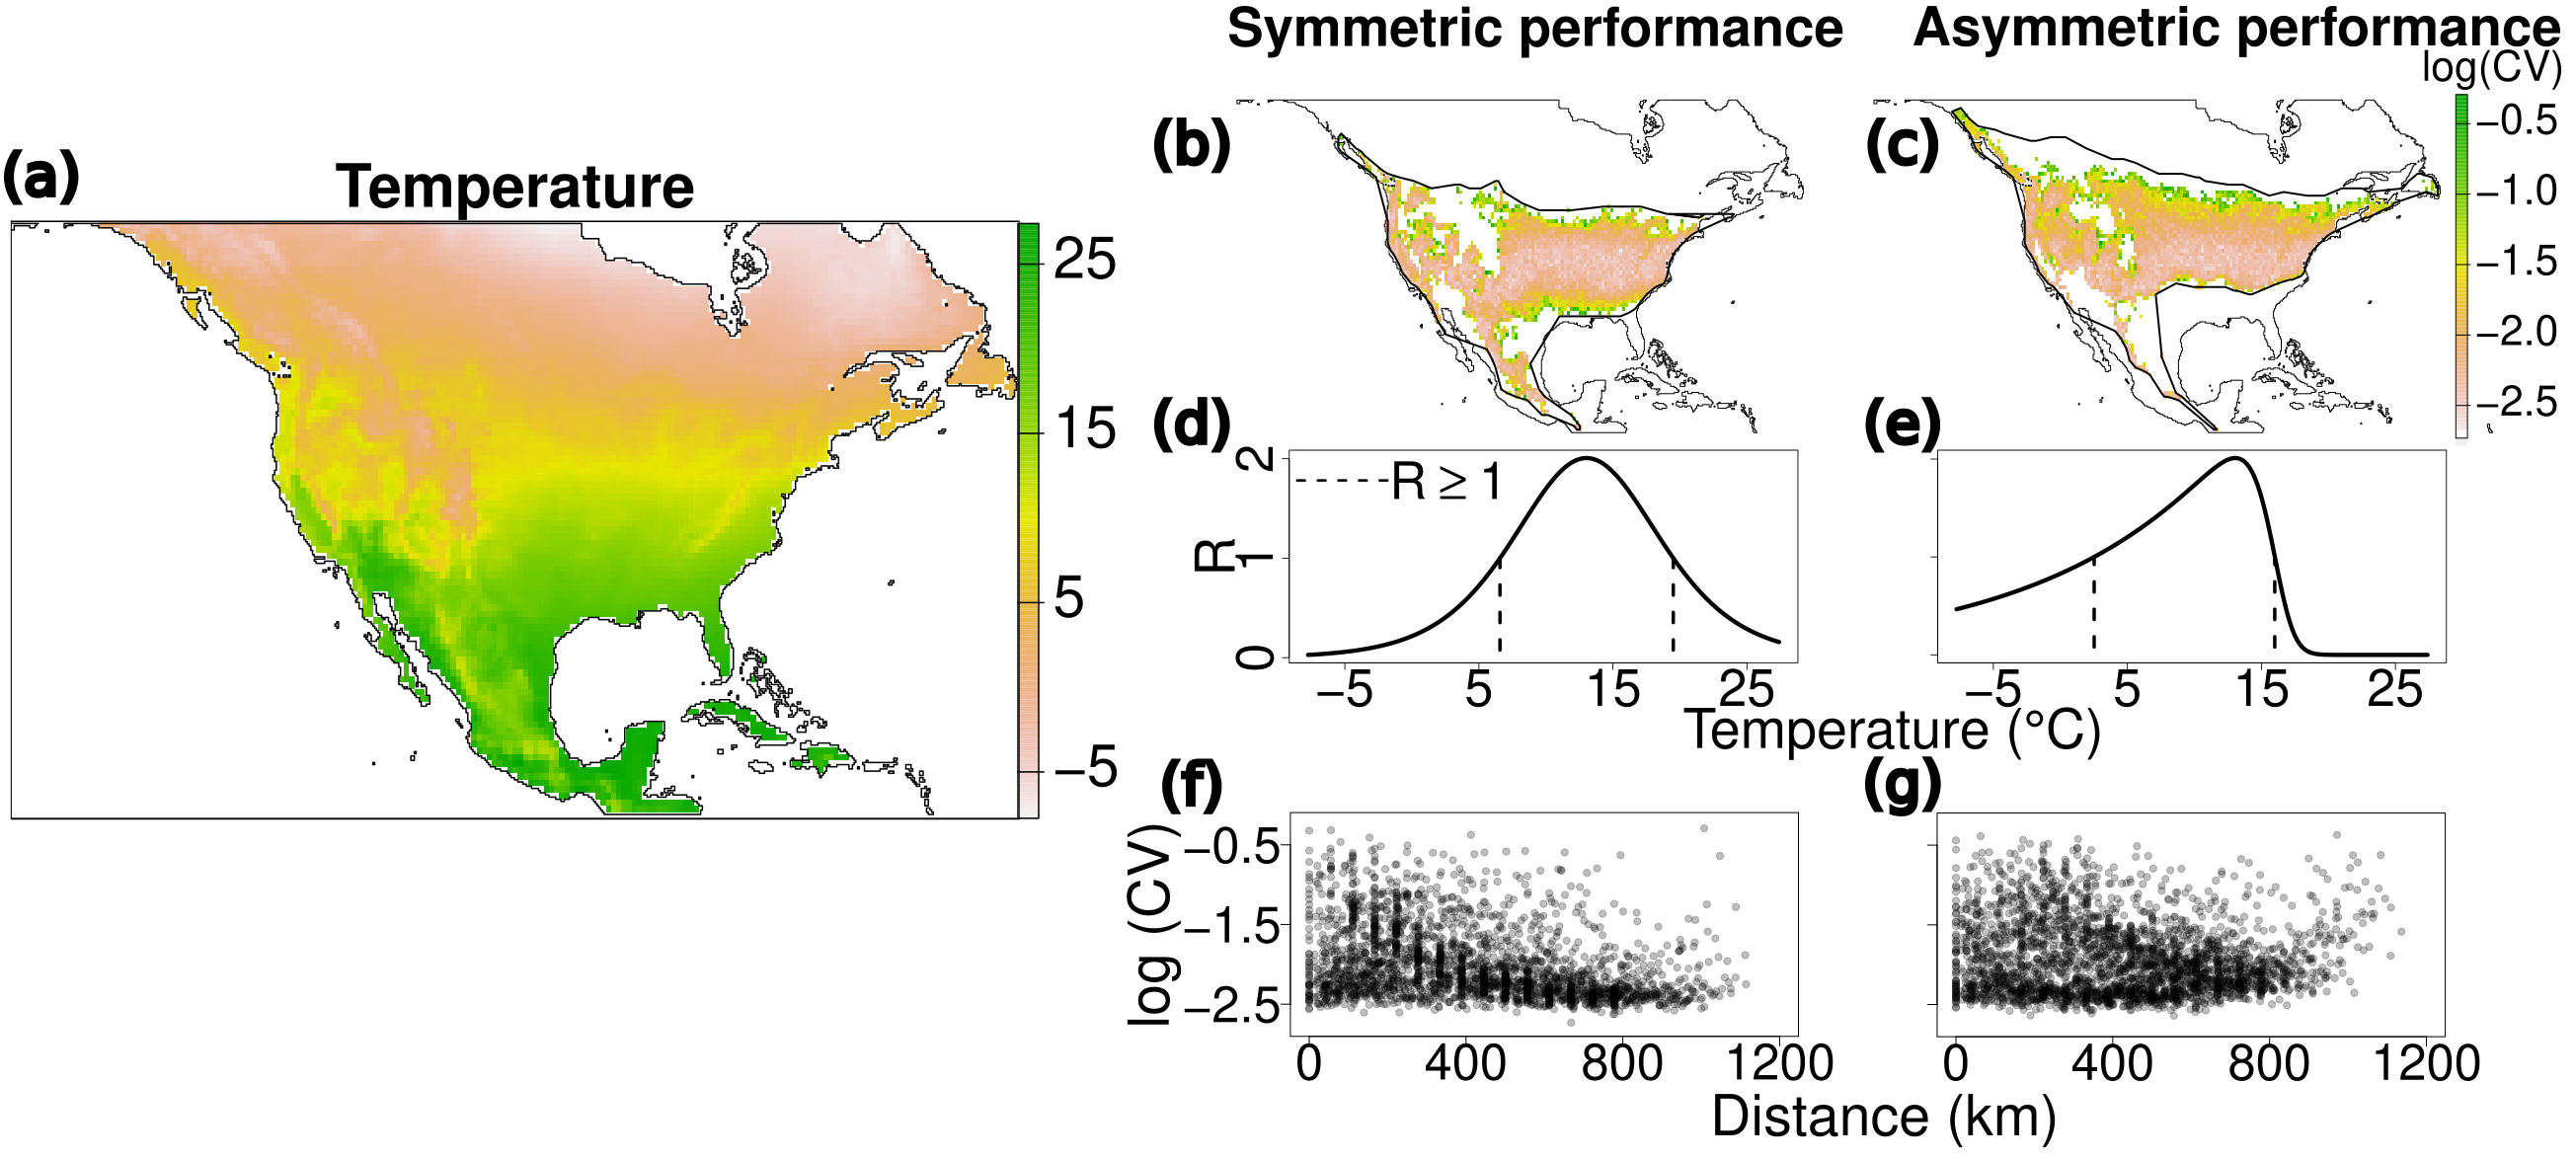
\includegraphics[width=1.025\linewidth]{teste3.png}%
\end{center}
\captionof{figure}[Performance curves and population variability across geographic space]{North American landscape (a) used to simulate population dynamics and to estimate population variability of the species with symmetric (b, d, f) and asymmetric (c, e, g) performance curves.}\label{fig:spatvar}}

\end{tcolorbox}


The level of spatial autocorrelation that environmental variables show can further influence geographic patterns in population variability. Spatial autocorrelation varies across different environmental conditions (temperature and precipitation) and regions (lowlands and mountainous regions), which can affect landscape heterogeneity and population dynamics. Highly spatially autocorrelated environmental conditions can lead to more pronounced geographic patterns of population variability compared to environmental conditions with low spatial autocorrelation. Thus, an interplay between the shape of species performance curves and the level of spatial autocorrelation of the environmental conditions that affect species performances are likely to drive geographic patterns of population variability.     


\section*{\textbf{\uline{Potential effects of changing environmental conditions on population variability}}}
%\subsection*{Potential effects of changing environmental conditions on population variability}

The characteristics of species thermal performance curves vary across geographic space. Species occurring in tropical regions often have narrower performance curves and occur in areas that have environmental conditions closer to their optimum \parencite{kingsolver2017}. This suggests that tropical species might be more susceptible to changes and fluctuations in environmental conditions as they are closer to their maximum critical temperature than temperate species \parencite{deutsch2008, kingsolver2013, dowd2015} but see \parencite{vasseur2014}. This has prompted an interest in using performance curves to predict how climate change and environmental variability will affect species \parencite{sinclair2016, buckley2008, kingsolver2013, kingsolver2017, dowd2015}.  Overall, environmental variability is predicted to decrease species performance \parencite{dowd2015,kingsolver2017} and species occurring in mid latitudes might be particularly susceptible changes and variation in environmental conditions \parencite{kingsolver2013, buckley2022}. Even small changes in the mean and in the variability of environmental conditions can be detrimental for tropical species \parencite{dowd2015, kingsolver2017} while temperate species are exposed to higher environmental variability that also negatively impacts their performance \parencite{huey2012, kingsolver2013}. This shows that changing environmental conditions can negatively affect species performances in different ways depending where species occur. 

Here, our goal is to demonstrate that species performance curves can also be used to understand patterns of population variability in constant and variable environments and how that can influence geographic patterns of population variability. We simulated population dynamics of two hypothetical species following the same framework described in Box 1, but we considered two different scenarios. In one scenario, population dynamics were simulated in a constant environment where environmental conditions did not vary from generation to generation. In the other scenario, we simulated an instance where there is environmental variability occurring from generation to generation following a normal distribution $N \sim (0, 3)$, and we assumed that populations would respond immediately to these fluctuations in environmental conditions. If environmental variability caused a population to go extinct at some point before the end of the simulation, we calculated population variability considering the individuals up until the extinction occurred.  

Some populations vary more than others because of their position within the species performance curves (Figure \ref{fig:envvar}). Populations found in less suitable environmental conditions (i.e., in environmental conditions where growth rate is $\approx$ 1) are naturally more variable regardless of the performance curve shape when environmental conditions are constant (Figure \ref{fig:envvar}). This occurs because these populations have lower growth rates and demographic stochasticity becomes an important driver of population variability in these cases. This suggests that as mean climatic conditions change over time, patterns of population variability within geographic ranges will also change. Variability in environmental conditions is predicted to increase with climate change \parencite{vasseur2014,kingsolver2017}, and in these cases population variability will increase especially for populations found near optimum conditions (Figure \ref{fig:envvar}). These results show that decreases in performance caused by environmental variability \parencite{dowd2015, kingsolver2017} are reflected in the higher variability of population densities. This is an example of Jensen's inequality, where despite average environmental conditions being the same in the constant and variable scenarios, fluctuating environments lead to more variable populations because of the disproportionate effects that positive and negative values of environmental variation have on growth rates \parencite{ruel1999, vasseur2014}. This suggests that environmental variability can obscure patterns of population variability across geographic ranges particularly for species that occur in areas with high environmental variability (e.g., temperate regions). 


\begin{figure}[H]%it was [ht] before, it is [H] now to force the figure to be here
\centering
\centerline{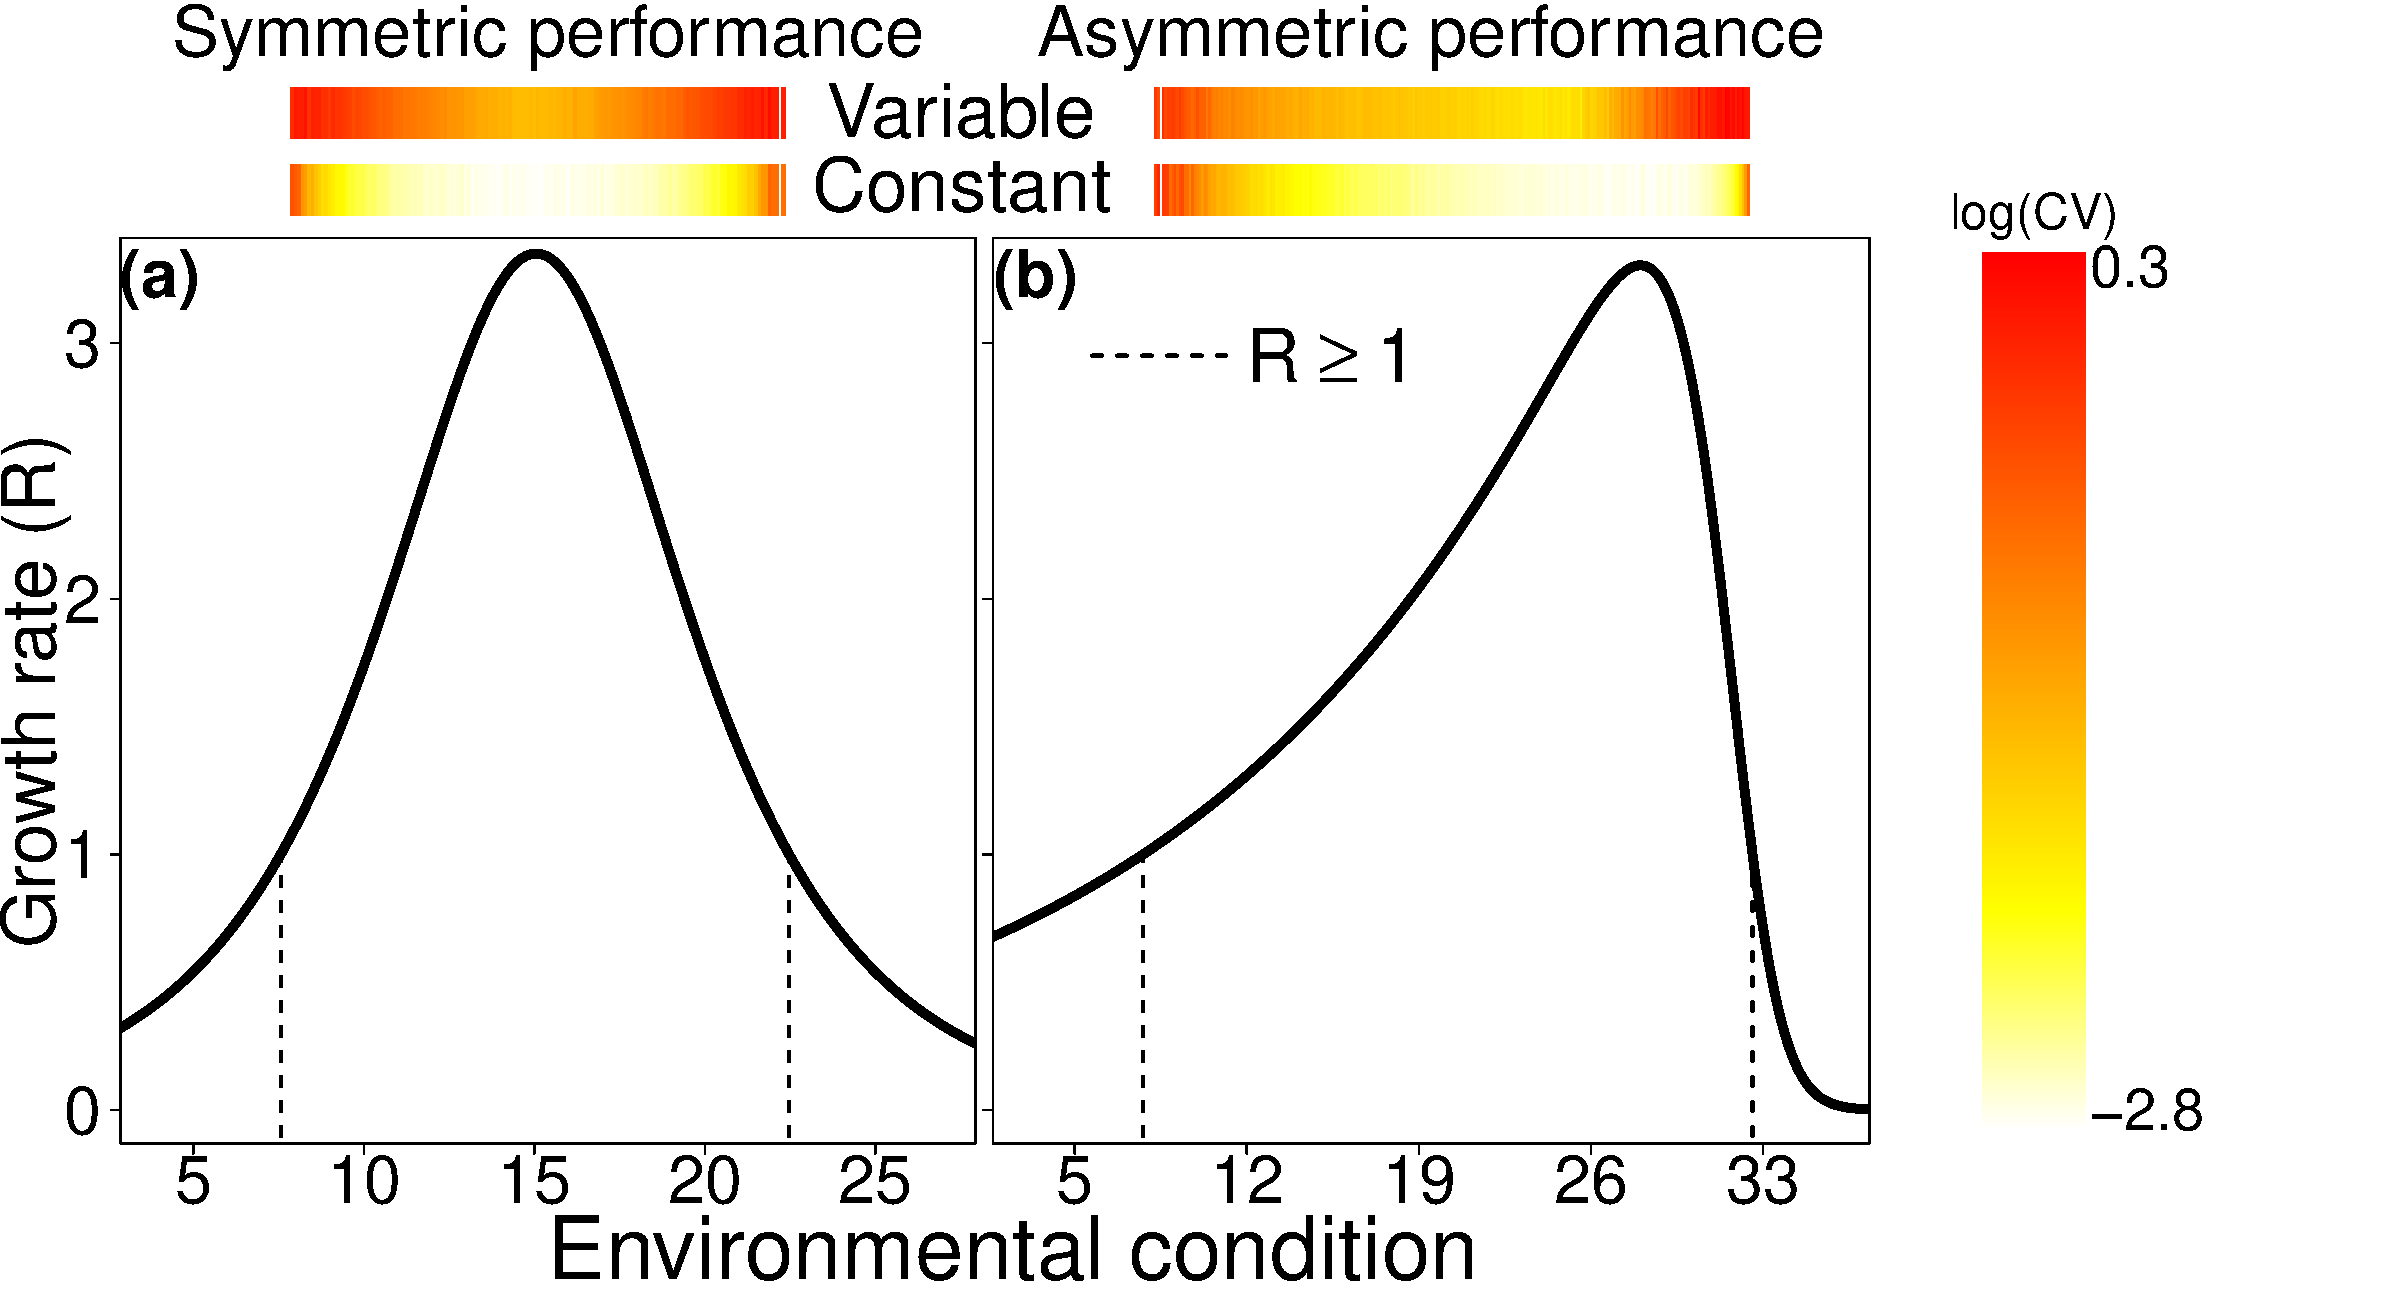
\includegraphics[width=1\textwidth]{FigRev/Env_Var}}
\caption[The effects of environmental variability on population variability]{Population variability estimates considering 200 generations for species with symmetric (a) and asymmetric (b) performance curves that have populations occurring along an environmental gradient.} 
\label{fig:envvar}
\end{figure}


Although our simulations were not spatially explicit (i.e., there was no dispersal occurring between populations), our results indicate that coupling information on species performance curves and environmental variability can improve our understanding of geographic patterns of population variability. This framework addresses the problem that populations found at edges of geographic ranges can be occurring in optimum environmental conditions \parencite{sheth2018, oldfather2019}, and could explain the lack of consistent geographic patterns of population variability across different species. Future changes in mean environmental conditions, alongside increased environmental variability, will contribute to form complex geographic patterns of population variability as this will reshuffle the position of populations along species performance curves. 
	

%\subsection*{Moving forward on the evaluation geographic patterns of population variability}
\section*{\textbf{\uline{Moving forward on the evaluation geographic patterns of population variability}}}

Describing geographic patterns of population variability is challenging because of the multiple intrinsic and extrinsic factors that cause fluctuations in population densities. Predictions of population variability based on geographic range position are appealing for their simplicity, but they have several limitations because of their simplifying assumptions, such as that geographic ranges are static and that environmental conditions are constantly unsuitable in range edges. Shifts in species geographic distributions and population dynamics at different parts of their geographic ranges because of ongoing changes in environmental conditions challenge these assumptions  \parencite{sheth2018,lewis2023,lawlor2024}. Dispersal and colonization processes affect population dynamics and the ability of species to occupy suitable environments across geographic space. This occurs, for example, for species that are invading new areas \parencite{vaclavik2012}, further highlighting the limitations of using geographic range position as a predictor for population variability. Performance curves overcome these problems and addresses assumptions that environmental conditions are spread in a specific way across geographic ranges and that ranges are static. Performance curves have been used to predict current and future geographic distribution of species \parencite{buckley2008,angilletta2009}, and we show that they are also useful to understand geographic patterns of population dynamics. 

Using performance curves allows one to disentangle geographic patterns of population variability, but there are some potential drawbacks with the use of this approach. Information on performance curves are not readily available for several species, and most of the research on this topic has been focused on thermal performance curves of ecthoterms \parencite{deutsch2008,angilletta2009,vasseur2014, dowd2015,kingsolver2017} while knowledge on endotherms' and plants' performance curves is generally lacking. This could pose some constraints on the use of performance curves to understand geographic patterns of population variability, but this limitation could be eventually overcome as descriptions of endotherms' and plants' performance curves become more widely available. Recent modeling frameworks are able to predict species performance curves from response trait data rather than from population-level information \parencite{simon2024}. Such framework can be used to address knowledge gaps for species where trait response data are more broadly available, but that we have limited knowledge on their performance curves. Another potential limitation of our approach is that we define performance curves at the species level, which may not be able to capture local adaptations exhibited by different populations \parencite{herrando2019,cicchino2023}. This problem can be overcome by sampling individuals from different populations, to account for potential local adaptations, when describing species performance curves. Below we outline some important next steps that could be considered in the study of geographic patterns of population variability: 

\begin{enumerate}
\item How does dispersal affect geographic patterns of population variability? Theoretical models predict that dispersal should reduce population variability, but empirical evidence suggests that the effects of dispersal on population variability are more complex.
\item How does microclimatic conditions affect population variability trends across geographic ranges? Coarse environmental predictors are often used to assess the role of environmental conditions on population dynamics, but microclimatic conditions can provide suitable environments and buffer population variability in areas that are seemingly unsuitable for a species.   
%\item Local adaptations
\item What is the role of biotic interactions in shaping geographic trends of population variability? Are the effects of antagonistic and mutualistic interactions on population variability similar in different parts of species geographic ranges?
\item What is the influence of temporal and spatial sampling scale on geographic patterns of population variability? Different patterns of population variability could be observed depending on how abundance data is aggregated in geographic space and how long populations have been sampled. 
\item How does periodic environmental variability affect population variability across geographic ranges? Seasonal fluctuation in environmental conditions can lead to variation in populations because of seasonal demography that species can exhibit.  
\item How do differences in life-history traits affect geographic patterns of population variability for different species? Is there a relationship between intraspecific variability of life-history traits and population variability across geographic ranges?
\item Is the geography of occupied sites important to determine geographic patterns of population variability? Population variability across geographic ranges could be explained by the size and the amount of resources that sites where populations occur have. 
\item Are there taxonomic differences in how populations vary across geographic ranges? Some taxa can have more or less variable populations across geographic ranges because of their ability to track suitable environments across geographic space. 
\item How is global change influencing population variability across geographic ranges? Species are shifting their geographic ranges because of changing environmental conditions, but it is unclear how population variability of these species is being affected by global change.  
\item How do different factors interact to drive geographic patterns of population variability? For example, changes in environmental conditions can modify the effects of species interactions on population dynamics, highlighting the importance of considering how different drivers of population dynamics might interact across geographic space to regulate geographic patterns of population variability.  
\end{enumerate}


Geographic patterns of population variability have often been evaluated using observational data. However, the use of theoretical models and controlled experimental approaches are needed to further our understanding of geographic patterns of population variability. For example, the role of species interactions or dispersal on spatial patterns of population variability can be challenging to assess with observational data, but these factors can be more easily considered in simulation studies and mesocosm experiments. A thorough understanding of geographic patterns of population variability will be obtained when theoretical models are coupled with experimental approaches and observational data to fully disentangle the role of different factors in driving geographic patterns of population variability.

                         %% Introduction.tex should begin

\addtocontents{toc}{\protect\vskip-20pt}
\chapter[The influence of geographic ranges, climatic niches, and temperature fluctuations on population variability.]{The influence of geographic ranges, climatic niches, and temperature fluctuations on population variability.\footnote[3]{Submitted to \textit{Proceedings B} as: Ten Caten, C., \& Dallas, T. The influence of geographic ranges, climatic niches, and temperature fluctuations on population variability.}}   

\setcounter{page}{76} %This does the trick

\section*{\textbf{\underline{Abstract}}}
The existence of patterns in population dynamics across species geographic ranges and climatic niches is a pervasive idea in ecology. Population variability (i.e., temporal variability in population density) should hypothetically increase near range edges or niche limits because of less suitable environments in these areas, but the occurrence of such patterns remains largely unexplored. Further, fluctuations in temperature could pose demographic constraints on populations and also influence their variability. We used the Breeding Bird Survey data to show that the population variability of 97 resident North American birds consistently increases towards their niche limits and in areas with more variable temperatures, but not towards their geographic range edges. However, our model has limited explanatory power, suggesting that other factors, such as biotic interactions and resource availability, might be more important drivers of population variability in resident North American birds.
%-----------------------
\section*{\textbf{\underline{Introduction}}}
%\section*{Introduction}
A general goal in ecology is to understand how species densities changes across geographic space and over time \parencite{lundberg2000,borregaard2010}. A commonly reported trend is that populations are more abundant the closer they are to the species geographic range center \parencite{brown1984, sexton2009}. Species climatic niches (i.e., the range of environmental conditions that allow species to persist indefinitely) are a main factor limiting species geographic distributions \parencite{pulliam2000, colwell2009}, such that these environmental conditions are assumed to be closer to the species optimum in the center of their geographic ranges, leading to higher density in these areas \parencite{brown1984,sagarin2006, pironon2017}. Despite being once regarded as a general rule \parencite{hengeveld1982}, evidence for the occurrence of geographic patterns in population density is limited \parencite{sagarin2002, sagarin2006, pironon2017, dallas2017}. This lack of support for these geographic trends could be occurring because geographic edges do not reflect climatic niche limits for many species \parencite{oldfather2019, pennington2021}, leading to the suggestion that population dynamics are more related to the position of populations within the species climatic niche \parencite{martinez2013,osorio2020}.  

\paragraph*{}
Perhaps a less explored consequence of patterns of population density across geographic and niche space is that population dynamics would be more variable the closer populations are to the edges of geographic ranges and climatic niches \parencite{lawton1993,sagarin2006, pironon2017}. As these populations would have lower densities, demographic stochasticity becomes an important driver of their dynamics, leading populations to be more variable near range edges or niche limits \parencite{melbourne2008, pironon2017, tencaten2025}. Understanding how populations vary across species geographic ranges and climatic niches is of particular importance given that increasing fluctuations in population densities are associated with higher extinction risk \parencite{bjornstad2001, ovaskainen2010}, and the detection of such trends could inform conservation efforts \parencite{burgess2020}. However, differences in how population variability is structured across geographic ranges or climatic niches have rarely been assessed \parencite{sagarin2006,pironon2017, tencaten2025} despite being considered prevalent across species \parencite{vucetich2003}.
 
\paragraph*{}
Different extrinsic (environmental) and intrinsic (demographic) factors may affect population variability irrespective of population position within the species climatic niche or geographic range. For example, increased fluctuations in environmental conditions lead to more variable population dynamics given that extreme environments are more likely to pose demographic constraints on populations \parencite{bjornstad2001, boyce2006}. Species traits, such as body size and dispersal ability, may also influence patterns of population variability across geographic and climatic space. For instance, fluctuations in population densities are often associated with changes in body sizes \parencite{chitty1952,van2017} while dispersal usually stabilizes population dynamics \parencite{doebeli1995,abbott2011}. Several of these traits that affect population dynamics are phylogenetically conserved \parencite{wiens2010, park2015}, indicating that there could be a phylogenetic signal in patterns of population variability \parencite{dallas2024}.
 
\paragraph*{}
The influence of geographic ranges and climatic niches on population variability represents a major knowledge gap in our understanding of population dynamics. Differences in environmental conditions that populations experience are considered important drivers of patterns of population dynamics across geographic ranges and climatic niches \parencite{sagarin2006,pironon2017, tencaten2025}, but the effects of environmental factors are often ignored during the assessment of these relationships. Here we address these gaps and examine the effects of climatic niche position, geographic range position, and temperature variability on the population variability of 97 resident North American bird species (Figure \ref{fig:concep_varrange}). Phylogenetic history and species differences in body size and dispersal ability were considered to assess their influence on these relationships. We hypothesized that population variability would be more strongly related to climatic niche position and temperature variability than geographic range position. We expected this given that niches impose boundaries to the climatic conditions where populations can have positive growth rates and because temperature fluctuations can move populations along the species niche, and in some cases even beyond niche limits, influencing their variability. Alternatively, geographic range edges might not represent niche limits (Figure \ref{fig:rangelimits}) and can have suitable environmental conditions that could buffer population variability \parencite{oldfather2018}. We also expected that closely related species were going to exhibit similar patterns of population variability, and that species body size and dispersal ability would influence these relationships.  
 
%-----------------------
\section*{\textbf{\underline{Methods}}}
%\section*{Methods}
\paragraph*{Estimating population variability}\mbox{}\\ 
We used the North American Breeding Bird Survey (BBS; \textcite{sauer2020}) data to estimate yearly densities of 99 resident bird species. Species sampled by BBS were classified as resident based on \textcite{rosenberg2019}. The BBS is an annual standardized census of North American breeding birds. The surveys are conducted by skilled volunteers during the breeding season where survey routes of $\approx$ 50km are sampled every 1km (i.e., a total of 50 stops) for about 3 minutes through point counts where all birds seen or heard within a 0.4km radius are recorded. We only considered resident species because migratory birds might be exposed to different environmental conditions in their breeding and non-breeding ranges \parencite{ponti2020} that could affect their survival. Many migratory birds also have a substantial portion of their geographic ranges in areas outside of North America that are not sampled by BBS. Resident species could still have only a small portion of their geographic ranges sampled by BBS, but restricting our analysis to consider only resident species that had $\geq$70\% of their geographic ranges sampled by BBS yielded the same results as when considering all resident species (see Appendix C for details). BBS data was obtained through the \texttt{bbsAssistant} R package \parencite{burnett2019}.


We used the data sampled between 1997 and 2019 to estimate population variability for the  species considered in our study. The species considered in our study have been recorded in a total of 4803 routes since 1997. Each route has been sampled on average for 15$\pm$7 years and an average of 3051$\pm$127 routes were surveyed by BBS yearly between 1997 and 2019 (Figure \ref{fig:routes}). Population variability was estimated as the coefficient of variation (hereafter CV; $CV = \frac{\sigma}{\mu}$), relating the standard deviation in temporal dynamics of a population ($\sigma$) to it's mean ($\mu$) in density in a site. Only sites where species were recorded for at least five different time periods (mean of 371$\pm$600 sites) were considered in our calculations. Population variability was estimated considering only the years a species was observed to occur in a target site. We also explored whether a more conservative estimate of population variability, only considering sites where species were observed to occur in at least 10 years, influenced the observed relationships. Alternatively, we also considered a less conservative estimate of population variability, where we assigned a density of zero to sampling events where a species was not recorded in a site, but that sampling event was done between the first and last year that a species was recorded at a given site to investigate whether this assumption affects our results. %In this case, it is possible for a species that was observed five times in a site to have density of zero for three years and density > zero for the two other years. 

\paragraph*{Estimating geographic ranges, realized climatic niches, and temperature variability}\mbox{}\\ 
We estimated species geographic ranges as minimum convex polygons considering all BBS sampled points. The minimum convex polygon is defined as the smallest area that connects all sampled points that a species was recorded at with no interior edge. We opted to build our own polygons rather than using expert-derived ranges because of potential problems associated with using expert ranges. For example, expert estimates of a species geographic range can be disjunct, which can lead to the center of the range falling outside the species geographic range and there might also be observations that fall outside of expert ranges  \parencite{fristoe2023}, which could affect the assessment of these relationships. The center of the species geographic range was defined as the centroid of the species ranges. Geographic range centers were also estimated using expert ranges obtained from birdLife \parencite{birdlife} rather than minimum convex polygons and we also used distance to range edge as an alternative measure of geographic range position and found similar results (see Appendix C). 


To estimate the realized climatic niche of the species in our study, we used the 19 bioclimatic variables, consisting of quantities related to temperature and precipitation relevant to species life history (e.g., temperature seasonality, temperature of coldest month, etc.), available in the CHELSA database \parencite{karger2017}. These variables are considered main drivers of North American birds distribution and abundance \parencite{barbet2014, illan2014, huang2017}. Bioclimatic variables were obtained at a resolution of 0.008$^\circ$, and were aggregated to 0.5$^\circ$. to match the resolution of sampled BBS sites. We performed a principal component analysis (PCA) over these variables, and used the first two axes (explained $\approx$ 80\% of the variance in the data) to estimate realized climatic niches. We extracted environmental values from these two PCA axes and used minimum convex polygons to determine species realized climatic niches (see Figure \ref{fig:concep_varrange}). The centroid of these polygons were used to represent the center of climatic species niches. Climatic niches were also estimated using expert ranges and we observed similar results (see Appendix C for details).  

To estimate temperature variability, we obtained monthly mean temperature data for the years of 1997-2019 also from CHELSA database at a resolution of 0.008$^\circ$. that were aggregated to 0.5$^\circ$. To account for the different number of cells potentially being aggregated across different latitudes due to conformal projection, we also reprojected and aggregated mean monthly temperature data using Behrmann equal area projection (see details in Appendix C). We estimated the coefficient of variation in temperature for each year and site where species were sampled to use as an estimate of temperature variability that populations experienced. 
\paragraph*{The relationship between population variability and geographic ranges, climatic niches, and temperature fluctuations}\mbox{}\\ 
To evaluate how population variability was related to geographic range position, niche position, and temperature variability we fit linear mixed models. Two species (\textit{Strix nebulosa} and \textit{Megascops kennicottii}) that were sampled in fewer than five sites for at least five years were removed from our analyses. Population variability was the response variable and geographic range position, climatic niche position, and mean annual temperature variability were fixed effects in these models. Species were used as random effects (considering a reduced-rank covariance structure) to estimate the slope of the relationship between population variability and the fixed effects for each species separately. Thus, our models had random slopes, but not random intercepts, as random effects. All variables were standardized to have a mean of zero and a standard deviation of one prior to fitting the models. Linear mixed models were fit using a Gaussian family with the \texttt{glmmTMB} R package \parencite{brooks2017} and we performed model diagnostics (see Figure \ref{fig:main_mod} and Appendix C for details) and estimated model goodness of fit (Nakagawa's conditional $R^2$) using the \texttt{performance} R package \parencite{ludecke2021}. This conditional $R^2$ takes fixed and random effects into account when estimating the model goodness of fit.
\paragraph*{Assessing the effects of phylogeny and species traits on patterns of population variability}\mbox{}\\ 
Information on body size and dispersal ability for each species was obtained from the AVONET database \parencite{tobias2022}. We used body mass as a measure of body size and the hand-wing index as a measure of dispersal ability. Measuring the dispersal ability of birds is a challenging task, and for that reason biometric indices have often been used to describe their dispersal ability \parencite{sheard2020}. The hand-wing index considers information on flight efficiency and metabolic demands \parencite{claramunt2012,claramunt2017} and is positively related to the dispersal ability of birds \parencite{arango2022}. We used the crosswalk taxonomy from AVONET \parencite{tobias2022} to link the taxonomies from BirdLife and BirdTree \parencite{jetz2012bird} to obtain phylogenetic information for the 97 resident species considered in our analyses. We removed \textit{Aphelocoma woodhouseii} from our phylogenetic analyses because its equivalent species in BirdTree was a duplicate in our dataset (i.e., it was already present in our dataset). Thus, the phylogeny we used to assess whether species traits affect trends in population variability had 96 species.

We extracted the random slopes for each species from our linear mixed model and estimated Pagel's $\lambda$ and Blomberg's $K$ to assess whether there is a phylogenetic signal in how population variability is structured as a function geographic range position, climatic niche position, and temperature variability across species. Phylogenetic signal was estimated using the \texttt{phytools} package \parencite{revell2012}. We also fit three phylogenetic generalized least squares (PGLS) to explore how the species slopes changed as a function of log-transformed body size and log-transformed dispersal ability. PGLS models were fit using the \texttt{caper} R package \parencite{caper}.

%-----------------------
\section*{\textbf{\underline{Results}}}
%\section*{Results}
\paragraph*{Is population variability related to geographic range position, climatic niche position, or temperature variability?}\mbox{}\\ 
We found that the population variability of resident North American birds increases near climatic niche limits and in areas that have more variable temperature (Table \ref{tab:lmm_main}). These results were consistent regardless of how population variability, climatic niches, and temperature variability were estimated (see Appendix C). The relationship between population variability and geographic range position was inconsistent and depended on how population variability was estimated, but not on how geographic ranges or range position were estimated (Tables \ref{tab:lmm_exp}-\ref{tab:lmm_edge} ). There was no relationship between population variability and geographic range position when population variability was estimated considering cases where species were observed at least five years in a site. However, these relationships became significant when zeros were considered when estimating population variability or when we only used populations that occurred in sites for at least 10 years (Tables \ref{tab:lmm_zeros}-\ref{tab:lmm_tens}). Nevertheless, conditional $R^2$ in our models were often $\approx$ 0.01, suggesting that most of the variance in these relationships remained unexplained. 

\paragraph*{Do phylogenetic history and traits affect population variability responses across species?}\mbox{}\\ 
There was no phylogenetic signal in the effects of climatic niche position ($\lambda  < 0.01, p = 1; K = 0.02, p = 0.81$) or temperature variability ($\lambda < 0.01, p = 1; K = 0.01, p = 0.92$) on population variability across species. There was some evidence for phylogenetic signal ($\lambda  < 0.01, p = 1; K = 0.10, p = 0.04$) in how population variability was related to geographic range position (Figure \ref{fig:phylo}). Species with smaller body sizes had less variable populations near geographic range edges, but not near niche limits or in variable temperatures while dispersal ability was unrelated to patterns of population variability. These models were unable to explain most of the variance in patterns of population variability across species ($R^2 \approx$ 0.1, Table \ref{tab:PGLS}). 
%-----------------------
\section*{\textbf{\underline{Discussion}}}
%\section*{Discussion}
Population variability is predicted to increase in areas that have unsuitable environmental conditions such as near geographic range edges and climatic niche limits or in climatically variable locations  \parencite{pironon2017,burgess2020,tencaten2025}, but there are limited empirical assessments of these expectations. We found that the population variability of resident North American birds consistently increases near climatic niche limits and in areas that have more variable temperatures, but not near geographic range edges. However, our models could not explain most of the variation in these relationships, and phylogenetic history and traits did not influence species differences in population variability. The limited explanatory power of these relationships may be because several factors, such as resource availability and biotic interactions, can simultaneously influence population variability \parencite{lundberg2000, tencaten2025}, which could obscure these patterns across geographic and niche space or in variable temperatures. The suitability of environmental conditions across geographic and niche space might also not exhibit a homogeneous gradient of more to less suitable conditions from center towards the edges of ranges or niches as previously suggested \parencite{brown1984, martinez2013}. This would lead to noisier relationships between population variability and their position within geographic and climatic niche space of species.  
  
\paragraph*{}
Increased population variability near climatic niche limits and in variable temperatures is possibly due to the harsh boundaries that niche limits impose on populations \parencite{sexton2009,hargreaves2014} and because temperature variability causes fluctuations in population growth rates and lead to more variable dynamics \parencite{lande1993}. Geographic range edges may represent physical barriers, such as mountains and terrestrial boundaries, and not niche limits for several species and can have suitable environmental conditions that might buffer population variability in these areas \parencite{oldfather2018,oldfather2019, pennington2021}. However, assigning a density of zero to sampling events where species were not recorded in sites or considering only sites that were sampled for over 10 year led to higher population variability near range edges. This suggests that sites that are only occupied temporarily by species influence observed patterns of population variability and that time series length might also be important to detect these relationships (\parencite{pimm1988}; see Appendix C for details). Nonetheless, individual populations can exhibit adaptations to local environmental conditions, and have different climatic niche limits, that could mitigate their variability \parencite{demarche2018,oldfather2019}. Such local adaptations, coupled with the occurrence of demographic compensation (i.e., opposing vital rate trends in different environments \parencite{doak2010,villellas2015}), might weaken the influence of climatic niche position, geographic range position and temperature variability on population variability.

\paragraph*{}
Species that have smaller body sizes often exhibit higher fluctuations in population density than larger-bodied species \parencite{lawton1994}, but we did not observe a consistent effect of body size on patterns of population variability. The inability of body size to explain species differences in patterns of population variability can be due to other factors (e.g., level of ecological specialization and habitat loss) possibly regulating the effects of body size on population dynamics \parencite{owens2000,cowlishaw2009}. Although dispersal of individuals influence population dynamics \parencite{doebeli1995, abbott2011}, species dispersal ability was unrelated to population variability patterns. Experimental evidence shows that, in many scenarios, dispersal does not affect population variability \parencite{yang2022}, indicating that dispersal ability may be unable to explain species differences in patterns of population variability. The lack of phylogenetic signal in these relationships also suggests that the factors that influence patterns of population variability are highly variable across North American bird species.

\paragraph*{}

The extent to which these findings are generalizable to other taxa is an interesting open question as the effects of geographic range position, climatic niche position, and temperature fluctuations on population variability may depend on life history traits. Considering the influence of species level properties on the strength of these relationships may also further our understanding of these macroecological patterns. For instance, do species with larger geographic ranges also tend to have more variable populations near range edges? How does climatic niche breadth influence these relationships? By leveraging population dynamic theory \parencite{roughgarden1975,levin1976}, along with ideas from physiological ecology about species performance curves \parencite{buckley2008,tencaten2025}, it may be possible to generate testable predictions from theory about where populations would be most temporally variable. Incorporating the effects of density-dependent processes, such as competition, when evaluating population variability patterns may further elucidate these macroecological relationships. \\

\section*{\textbf{\underline{Figures}}}

\begin{figure}[H]
\centering
\centerline{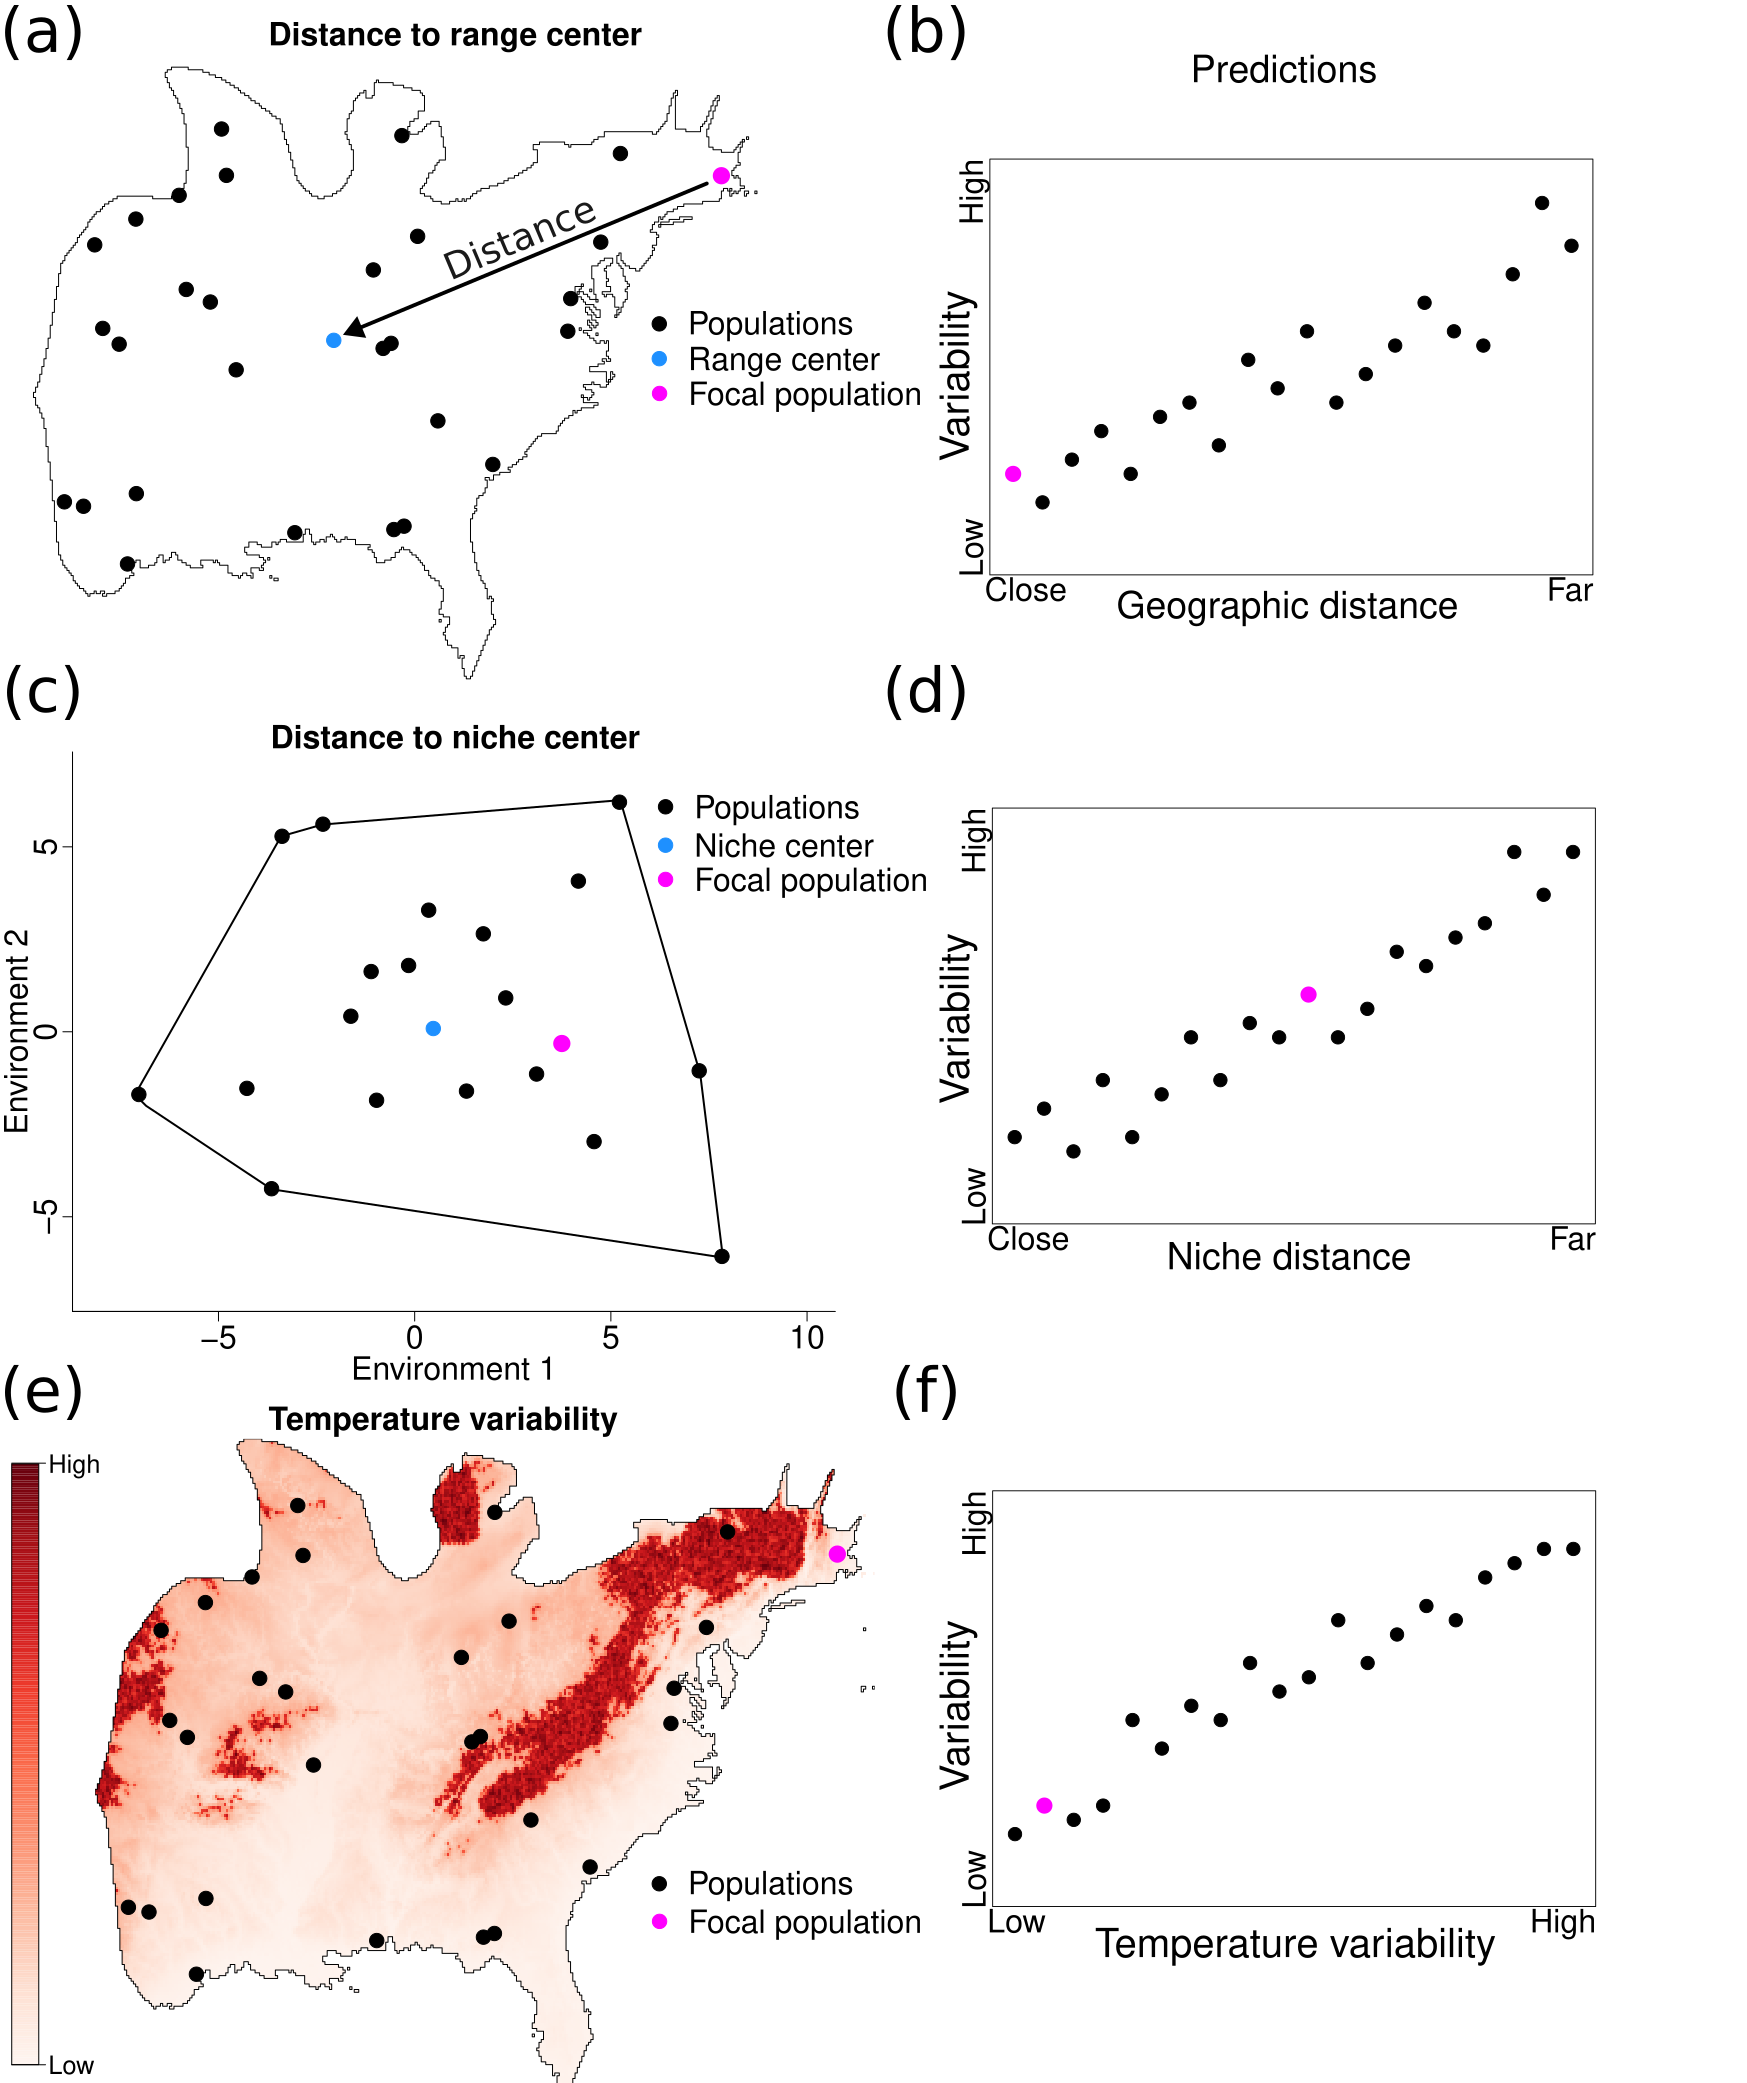
\includegraphics[width=1\textwidth]{FigRange/teste.png}}
\caption[Population variability across geographic and environmental space]{Population variability may be related to distance to geographic range center (a-b), distance to climatic niche center (c-d), or temperature variability (e-f).} 
\label{fig:concep_varrange}
\end{figure}

\begin{figure}[H]
\centering
\centerline{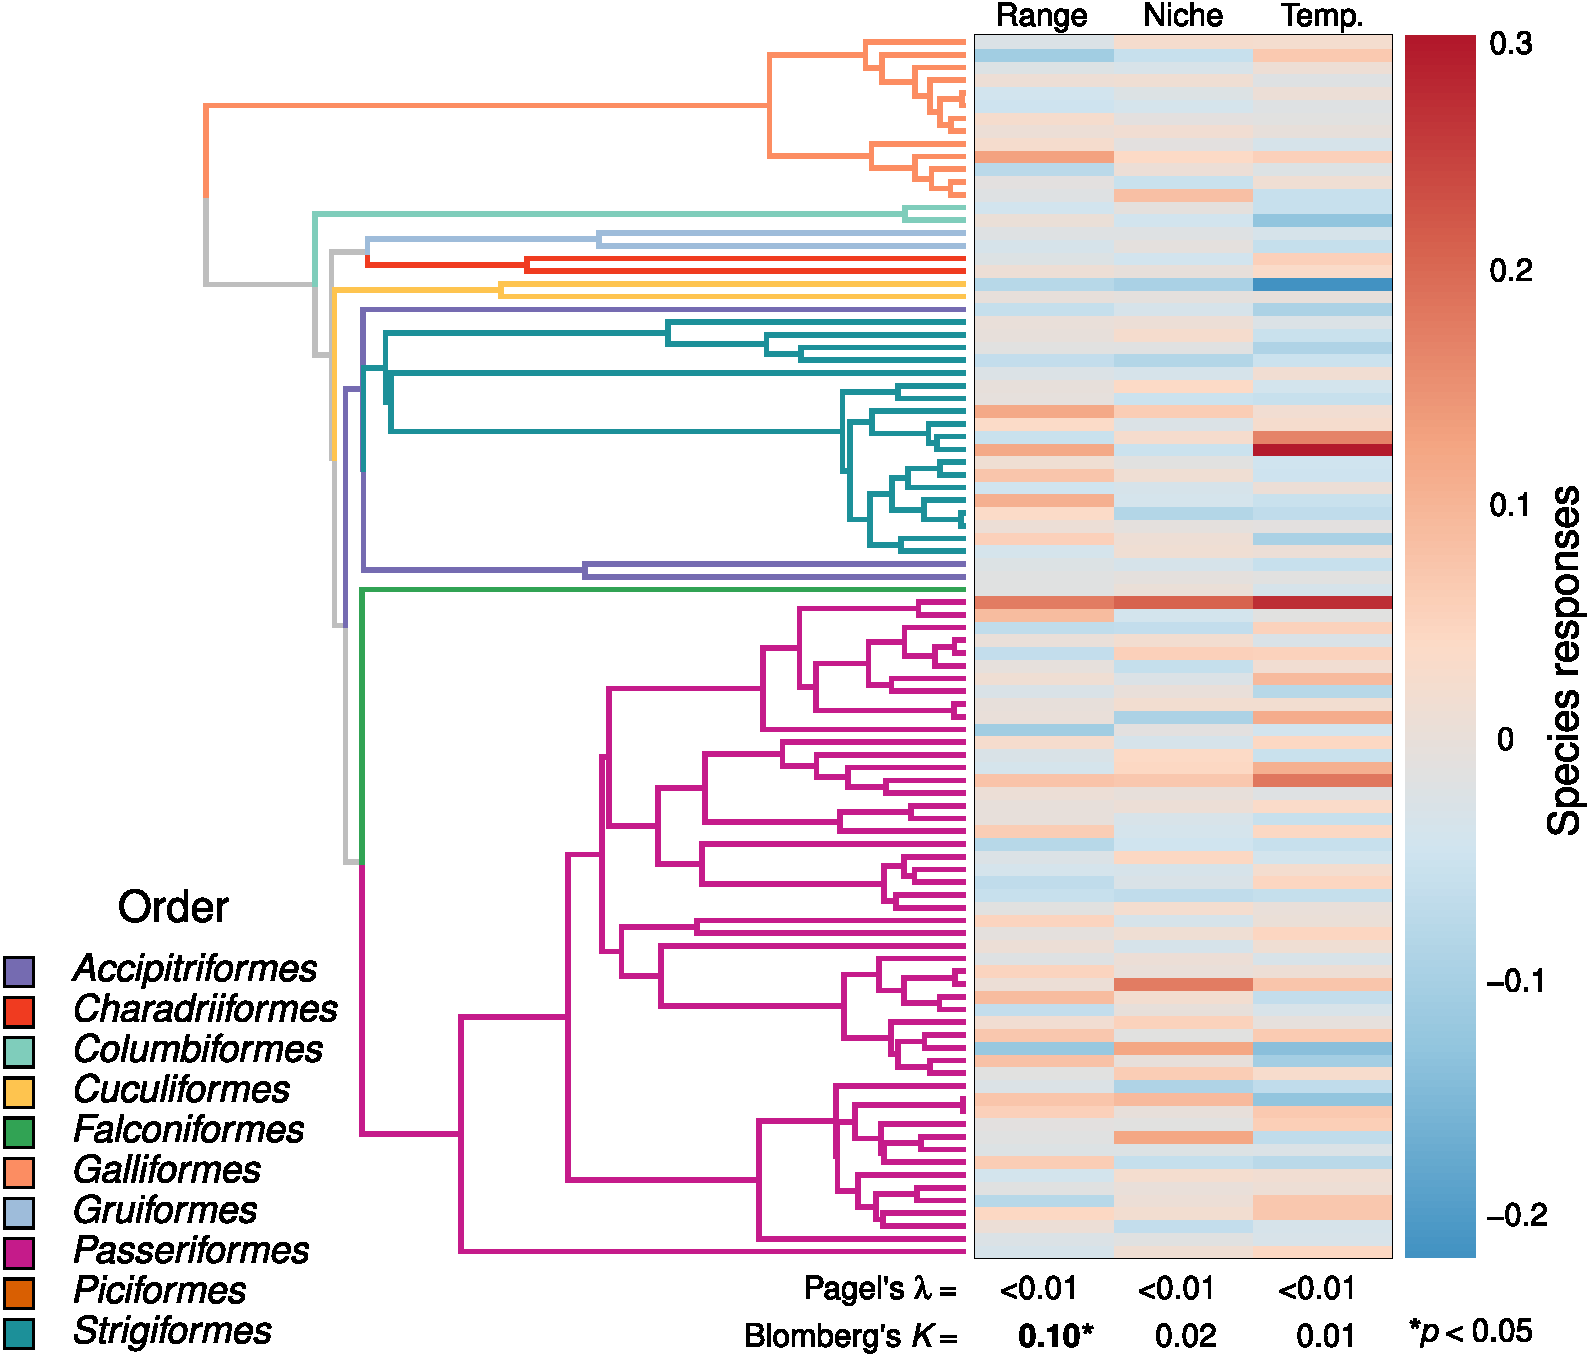
\includegraphics[width=1\textwidth]{FigRange/phyloplot}}
\caption[Phylogenetic signal on population variability]{There is no phylogenetic signal (Pagel's $\lambda$ and Blomberg's \textit{K}) in the relationship (Species responses) between climatic niche position (Niche) and temperature variability (Temp.) and population variability across species. However, there was some evidence for phylogenetic signal (Blomberg's \textit{K} = \textbf{0.10*}, p-value < 0.05) in the effects of geographic range position (Range) on population variability.} 
\label{fig:phylo}
\end{figure}

\section*{\textbf{\underline{Tables}}}

%\section*{Tables}
% latex table generated in R 4.3.2 by xtable 1.8-4 package
% Tue Jan 21 23:23:35 2025
\begin{table}[H]
\centering
  \caption[Results from linear mixed effect model]{Results from the linear mixed model showing that population variability increases near climatic niche limits (Niche) and in variable temperatures (Temp.) but not near geographic range edges (Range).}
  \vspace*{3mm}
\begin{tabular}{ccccc}
  \hline
 Predictor & Estimate & Std. Error & z value & Pr($>$|$z$|) \\ 
  \hline
  Intercept & 0.008 & 0.005 & 1.517 & 0.129 \\ 
  Niche & 0.044 & 0.013 & 3.516 & \textbf{<0.001} \\ 
  Range & 0.007 & 0.013 & 0.528 & 0.597 \\ 
  Temp. & 0.049 & 0.015 & 3.251 & \textbf{0.001} \\ 
   \hline
\end{tabular}
\label{tab:lmm_main}
\end{table}

% latex table generated in R 4.3.2 by xtable 1.8-4 package
% Wed Jan 22 08:09:11 2025
\begin{table}[H]
\centering
  \caption[Results from phylogenetic generalized least squares model]{Results from the phylogenetic generalized least squares showing the effects of body size (Body size) and dispersal ability (Dispersal) on patterns of population variability across geographic ranges (Range), climatic niches (Niche), and variable temperatures (Temp.).}
  \vspace*{3mm}
\begin{tabular}{ccccccc}
  \hline
Condition & Trait & Estimate & StdError & tvalue & pvalue & $R^2$ \\ 
  \hline
  \multirow{3}{*}[-.6ex]{\rotatebox{90}{Range}}   & Intercept & -0.025 & 0.039 & -0.637 & 0.526 & \\ 
   & Dispersal & 0.022 & 0.015 & 1.492 & 0.139 & 0.03 \\ 
   & Body size & -0.009 & 0.004 & -2.291 & \textbf{0.024} & \\\hline 
 \multirow{3}{*}[-.6ex]{\rotatebox{90}{Niche}}  & Intercept & 0.036 & 0.038 & 0.944 & 0.348 &\\ 
   & Dispersal & -0.006 & 0.014 & -0.439 & 0.661 & > 0.01\\ 
   & Body size & -0.004 & 0.004 & -0.930 & 0.355 & \\\hline 
 \multirow{3}{*}[-.6ex]{\rotatebox{90}{Temp.}}  & Intercept & 0.011 & 0.055 & 0.203 & 0.839 &\\
   & Dispersal & 0.006 & 0.021 & 0.309 & 0.758 & >0.01\\ 
   & Body size & -0.007 & 0.006 & -1.226 & 0.223& \\ 
   \hline
\end{tabular}
\label{tab:PGLS}
\end{table}

%\section*{Figures}
                         
\addtocontents{toc}{\protect\vskip-20pt}
\chapter[The effects of degree distribution on metapopulation size, variability, and persistence]{The effects of degree distribution on metapopulation size, variability, and persistence.\footnote[4]{In preparation as: Ten Caten, C., \& Dallas, T. The effects of degree distribution on metapopulation size, variability, and persistence.}}    %% Calls Introduction.tex


\section*{\textbf{\underline{Abstract}}}
The dispersal of individuals between spatially distributed populations is key for the maintenance of metapopulations and local populations. In this case, differences in the level of isolation of patches within spatial networks can have contrasting effects on their resulting dynamics, influencing the size, variability, and persistence time of metapopulations. We experimentally examined how the degree distribution of spatial networks influences the size, variability, and persistence of \textit{Daphnia} metapopulations. We found that spatial networks that are more heterogeneous have longer persistence times than homogeneous networks, but their size and variability is the same across different network types. At the local population level, patch degree did not influence the size, variability, and probability of a patch being occupied. These results suggest that degree distribution has complex effects on metapopulation dynamics.

%-----------------------
\section*{\textbf{\underline{Introduction}}}

The dispersal of individuals between spatially distributed populations has important effects on populations \parencite{hanski1998, abbott2011}, influencing colonization-extinction dynamics, the variability of local populations, and metapopulation persistence \parencite{wang2015,fox2017, schmidt2020}. The spatial distribution and distance between populations affect the probability of individual dispersal in spatial networks, such that individuals are less likely to disperse to more isolated populations, which can increase the extinction risk of these populations \parencite{brown1977, schmidt2020}. Population sizes also also play a key role in driving local dynamics, where smaller populations are more likely to vary and go extinct, even in homogeneous environments, because of demographic stochasticity \parencite{hanski1998,melbourne2008}. Dispersal of individuals may thus be crucial for the maintenance of small populations \parencite{sutherland2012}.
%to allow the persistence of species that have small population sizes
 
%The spatial distribution of populations across landscapes is an important determinant of local population dynamics through dispersal events \parencite{hanski1998}. Dispersal of individuals influence colonization-extinction dynamics, the variability of local populations, and metapopulation persistence \parencite{fox2017}. The spatial distance between populations affect the dispersal of individuals in these spatial networks, such that fewer individuals would disperse to more isolated populations leading to a higher extinction rates in these areas \parencite{macarthur1970, brown1977, schmidt2020}. Local population sizes would also influence these dynamics, such that smaller populations would be more likely to vary and go extinct, even in homogeneous environments, because of demographic stochasticity \parencite{hanski1998,melbourne2008}. This suggests that dispersal is particularly important to allow the persistence of species that have small population sizes \parencite{sutherland2012}.
\paragraph*{}
%Although small populations face higher extinction risk, the persistence of these populations in spatial networks can be enhanced through dispersal events that provide a continuous influx of individuals and prevent their local extinction, through the rescue effect, and enhance metapopulation persistence \parencite{brown1977, abbott2011}. Talk about panmitic patchy metapops here and how dispersal may vary in these cases? Classical metapopulation theory states that individuals can only disperse to some of the populations, but empirical evidence rarely support this, and instead, it seems that patchy panmitic metapopulations are common
Rare and common species, when occurring in ecologically marginal environments, have populations with low densities \parencite{brown1984, lawton1993}, such that small populations are prevalent in nature and represent a key component of biodiversity \parencite{preston1948,ehrlich1993}. Although small populations face higher extinction risk, dispersal can provide a continuous influx of individuals to small populations and prevent their local extinction in spatial networks, through the rescue effect, and enhance metapopulation persistence \parencite{brown1977, abbott2011}. The prevalence of dispersal events in spatial networks can widely vary to being relatively rare in classic metapopulations to being extremely common in patchy populations \parencite{elmhagen2001, ovaskainen2004, fronhofer2012}. Theoretical frameworks indicate that such differences in dispersal across networks can lead to substantially different dynamics in metapopulations and local populations \parencite{heino1997,abbott2011,gilarranz2012,wang2015}, though there is mixed evidence from empirical systems supporting these theoretical predictions \parencite{yang2022}. 

% In patchy populations dispersal events are frequent such that the same individual may reproduce in different patches during its life time \parencite{harrison1991, ovaskainen2004}. Patchy populations represent an interesting framework to understand the effects of isolation on population dynamics given that patches can vary in their degree of accessibility, but still be reachable by all individuals.% This would allow 
%Why are patchy populations interesting? 
% depending on the spatial structure of the local populations \parencite{} According to classic metapopulation theory, the dispersal of individuals between populations is a relatively rare event    However, high dispersal rates may promote synchrony between populations and might negatively impact metapopulation persistence by increasing the probability that local populations go extinct simultaneously \parencite{heino1997,abbott2011}. Although dispersal is predicted to decrease local population variability \parencite{abbott2011,wang2015}, experimental evidence supporting this expectation is contrasting, indicating that the effects of dispersal on local population variability may vary across taxa and depend on experimental length \parencite{yang2022}.  
%Experimental evidence show that taxa, number of patches, and experimental length influence the observed effects of dispersal on population dynamics \parencite{yang2022}, further highlighting that dispersal can have complex effects on population dynamics.  

\paragraph*{}
The spatial distance between populations across landscapes is often used to represent population isolation, but the degree distribution (i.e., number of connections that populations share in a network) also provides information on their level of isolation \parencite{schmidt2020,arancibia2021}. Populations occurring in real networks have different number of connections that directly influence their dynamics \parencite{hanski1998, arancibia2024}. For instance, metapopulations that have sites that are heterogeneous in their number of connections may be able to persist under a winder range of scenarios than homogeneous metapopulations \parencite{artzy2010, grilli2015}, though species life-history traits may affect how these dynamics unfold \parencite{gilarranz2012}. Local population dynamics can also be influenced by patch degree, where patches may be less variable and more often occupied when they are highly connected \parencite{gilarranz2012, arancibia2024}. This suggests that differences in network topology caused by how the number of connections are distributed across nodes, and consequently by how isolated patches are, can substantially affect metapopulation and local population dynamics even when everything else, such as resource availability and environmental conditions, remains constant.

%in metacommunities, a positive relationship between number of connections and community variability is observed when communities have a high variation in the number of connections, but not when the number of connections is similar across communities \parencite{arancibia2024}. 


\paragraph*{}
Here we experimentally examined how the degree distribution of spatial networks influences the size, variability, and persistence of \textit{Daphnia} metapopulations. These spatial networks were composed of  small extinction-prone populations that were identical, but could have one of three types of degree distribution (Figure \ref{fig:conceptual}). We hypothesized that metapopulations that were more heterogeneous in their degree distribution would be larger, less variable, and persist for longer periods of time than more homogeneous metapopulations. We also predicted that local populations would be larger, less variable, and more likely to be temporally occupied the more connections populations had. We found that spatial networks that are more heterogeneous have longer persistence times than homogeneous networks, but their size and variability is the same across different network types. At the local population level, patch degree did not influence the size, variability, and probability of a patch being occupied. 
% local variability would be lowest in populations that have an intermediate number of connections while metapopulation persistence would be enhanced in spatial networks where populations are variable in their number of connections. This was expected because intermediate dispersal is often suggested to reduce population variability \parencite{abbott2011} and because a high variation in number of connections may prevent synchrony between populations and enhance metapopulation persistence \parencite{arancibia2024}. We found.. 

%%%The environmental correlation of the patches may influence the effects of dispersal on population variabilioty


%estimate CV using all information and estimate it considering only cases when patches were occupied to see if results change. When using all data we may need to take the log?
%Degree distribution affected the variability of metacommunities when communities had a high variation in the number of connections, but not when communities had a similar number of connections \parencite{arancibia2024}.    where populations have on average the same number of connections the number of connectes  BREAK DOWN THIS PART

% Alternatively, increasing the mean number of connections between populations in a network may enhance metapopulation persistence \parencite{holyoak2000}, but can also promote synchrony between populations and increase metapopulation extinction risk \parencite{}. This indicates that number of connections can have a complex effect on metapopulation dynamics. 

%spatial networks that higher higher mean number of connections may have positive effects on metapopulation persistence promote synchrony between populations and increase metapopulation extinction risk \cite{refs}. 

%For instance, spatial networks where patches are equally connected may promote synchrony between populations and increase metapopulation extinction risk \cite{refs}. 

%  natural world isolation of populations in spatial networks are often 
%Although geographic distance between populations is often used to estimate the isolation of populations \parencite{schmidt2020}, populations may be more or less isolated depending on how many others are connected to them. Talk about degree distribution here


%Talk about network structure and degree in here. It has been not investigated that much in experiments and blablabla
%Early on theoretical models of patch networks considered all patches being equally connected, but this is not the case in real networks \parencite{hanski1998} 
% Isolation may not necessarily be measured by distance, but by the degree
 
%Local population dynamics are influenced by the spatial distribution of populations across geographic space, such that complex spatial dynamics can be observed even in the absence of environmental heterogeneity \parencite{hanski1998}. For instance, demographic stochasticity can be an important driver of population dynamics when population sizes are small, and that may to lead to complex extinction and recolonization dynamics occur  \parencite{melbourne2008,la,lw}. 

%end paragraph wioth dispersal

%Complex spatial dynamics in populations can be observed even in the absence \paragraph*{}
%This paragraph is about the effects of dispersal on meta population stability and persistence

%-----------------------
\section*{\textbf{\underline{Methods}}}

\paragraph*{Experimental system}\mbox{}\\
Our model species consists of a single clone of the freshwater cladoceran \textit{Dahpnia dentifera} reared on a mixture of filtered lake water and deionized water. To remove the potential confounding effects that individual age and maternal environment could have on vital rates, we isolated offspring from parthenogenetic females raised in isolation to obtain individuals of known age and maternal environment. Parthenogenetic females were individually placed into 50 mL test tubes filled with filtered lake water and deionized water, and were daily fed 50 $\mu$g  of a 2 g/L suspension (equivalent to 1 mg/L algal dry weight) of pulverized blue-green algae (\textit{Spirulina sp.}) and kept on the laboratory benchtop under a 12 hour light cycle. A total of 720 individuals that were 2-3 days old were obtained to seed the spatial networks (see details below).

%\textit{D. dentifera} were fed 50 $\mu$g  of a 2 g/L suspension (equivalent to 1 mg/L algal dry weight) of pulverized blue-green algae (\textit{Spirulina sp.}), and kept on the laboratory benchtop under a 12 hour light cycle.

%To remove the potential confounding effects that individual age and maternal environment could have on vital rates, we isolated offspring from parthenogenetic females raised in isolation to obtain individuals of known age and maternal environment. Parthenogenetic females were individually placed into 50 mL test tubes filled with filtered lake water and deionized water and were daily fed 50 $\mu$g  of a 2 g/L suspension (equivalent to 1 mg/L algal dry weight) of pulverized blue-green algae (\textit{Spirulina sp.}). We obtained 720 individuals that were 1-3 days old that where used in the 30 metapopulations that we considered in our study. 
\paragraph*{Spatial networks}\mbox{}\\
To examine how degree distribution influence local population dynamics and the persistence of \textit{D. dentifera}, we created three spatial network types (ten replicates per type; Figure 1) composed of 24 patches of size $\approx$ 2.5mL that had the same edge density (number of dispersal corridors, 36), but that the degree distribution (number of corridors per patch) changed across the spatial network types. In the first network type, the degree distribution was homogeneous across patches, and every patch was connected to three other patches (hereafter low networks, Figure \ref{fig:conceptual}a). In the second network type, there was some heterogeneity in the degree distribution, such that most patches were connected to to two or five other patches (hereafter mid networks, Figure \ref{fig:conceptual}b). In the third network type, the degree distribution was highly heterogeneous where patches widely varied in their degree, ranging from one to eight connections (hereafter high networks, Figure \ref{fig:conceptual}c).
 
The experiment started with all patches in the spatial networks being occupied by one individual, such that each network had 24 individuals at the beginning of the experiment. Spatial networks were fed pulverized blue green algae daily and kept under a 12 hour light cycle. The number of individuals in each patch was counted daily for 104 days, and a network was considered extinct when no individuals were detected in any patch for three consecutive days. We considered day 104 to be the extinction time of metapopulations that still had individuals up to that day. 
 
\paragraph*{Estimating the size, variability, and persistence of metapopulations}\mbox{}\\
Metapopulation size was estimated as mean number of individuals recorded daily in the networks until extinctions occurred. Metapopulation variability was calculated as the coefficient of variation
(hereafter CV$_{met}$ $CV = \frac{\sigma}{\mu}$), relating the standard deviation in the density of a metapopulation ($\sigma$) to it's mean ($\mu$) density. Metapopulation variability was estimated for spatial networks considering all sampling events until extinctions were observed. Lastly, metapopulation persistence was estimated as the number of days until a spatial network went extinct. At the patch level, we estimated mean population size, population variability using the coefficient of variation (hereafter CV$_{pop}$), and we estimated temporal occupancy as the fraction of days that patches were occupied by at least one individual. 


%Local population variability was estimated using coefficient of variation (hereafter CV; $CV = \frac{\sigma}{\mu}$), relating the standard deviation in the density of a patch ($\sigma$) to it's mean ($\mu$) density. 
%[\textit{Potential problem: Can we estimate population variability with a lot of zeros as in our case? What are alternative estimates we could use?}]. We calculated metapopulation persistence time (set to a maximum values of X for the metapopulations that persisted for the whole duration of the experiment) as number of days until metapopulation extinction.

The effects of spatial network type on metapopulation size, variability, and persistence was evaluated using linear mixed effect models. In these models, the size, variability (CV$_{met}$), and persistence time (number of days) of spatial networks were used as response variable and network type was used as fixed effect while replicate number was used as random effect. Linear mixed effect models were also used to assess how the number of connections that patches had was related to their mean density, their variability in density, and to their probability of being occupied over time.  In these models, the response variable was mean population density, population variability (CV$_{pop}$), and temporal occupancy while the fixed effect was patch degree and the random effects were replicate number and patch number. These linear mixed models were fit considering a Gaussian family with the \texttt{glmmTMB} R package \parencite{brooks2017} and we estimated model goodness of fit (Nakagawa's conditional $R^2$) using the \texttt{performance} R package \parencite{ludecke2021}. This conditional $R^2$ takes fixed and random effects into account when estimating the model goodness of fit. 

% local population variability and number of connections were assessed using a linear mixed model. In this model, population variability (CV) was the response variable and degree (number of connections a patch had) was the fixed effect. We used network type and replicate as random effects. This linear mixed model was fit considering a Gaussian family with the \texttt{glmmTMB} R package \parencite{brooks2017} and we performed model diagnostics (see Figure \ref{fig:main_mod} and Supporting Information for details) and estimated model goodness of fit (Nakagawa's conditional $R^2$) using the \texttt{performance} R package \parencite{ludecke2021}. This conditional $R^2$ takes fixed and random effects into account when estimating the model goodness of fit. [\textit{Potential problem: Unbalanced number of patches with different degrees in the analyses. Specifically: Degree of 1 = 60 patches, 2 = 210 patches, 3 = 290 patches, 4 = 30 patches, 5 = 110 patches, 6 and 8  = 10 patches. What to do about this? Maybe bootstrapping? idk}]


%-----------------------
\section*{\textbf{\underline{Results}}}

\paragraph*{}
We found that metapopulation size and variability did not differ between the different network types (Figure \ref{fig:met}a-b). However, the heterogeneity in the degree distribution of networks affected their persistence time. Specifically, high networks had a longer persistence time than low, but not than mid (Figure \ref{fig:met}c), networks such that this model explained 31\% of the variance in persistence time of metapopulations (Table \ref{tab:lmm_meta}). At the patch level, degree did not influence the size, variability, and probability of patches being occupied over time (Figure \ref{fig:pop}, Table \ref{tab:lmm_pop}). 


%-----------------------



\section*{\textbf{\underline{Discussion}}}
The effects of network topology on metapopulation dynamics has long interested ecologists who have often addressed these questions using theoretical models and simulation frameworks \parencite{artzy2010,gilarranz2012,grilli2015}. However, the extent to which the findings from such theoretical studies are generalizable to empirical systems has been rarely assessed (but see \textcite{arancibia2021, arancibia2024}). Here, we experimentally examined how differences in network topology caused by variations in how connections are distributed across patches in networks affect metapopulation and local population dynamics of \textit{Daphnia dentifera}. At the metapopulation level, we found support for the expectation that increasing heterogeneity in the number of dispersal corridors that local populations have enhances metapopulation persistence. However, metapopulation size and variability were not different across network types, suggesting that metapopulation persistence may not enhanced through increases in the size and reductions in the variability of metapopulations. At the local population level, we found that patch degree did not influence mean population size, population variability, or the probability of a patch being occupied, thus not supporting our expectations. %Cite models that predicted

\paragraph*{}

The effects of degree distribution on metapopulation dynamics can depend on species life-history traits, where species that experience high extinction probabilities have superior performance in heterogeneous compared to homogeneous networks \parencite{gilarranz2012}. This might explain the increase in persistence time that we observed in our experiment as the metapopulations considered were composed of small extinction-prone populations. This could be occurring because homogeneous networks may promote density-dependent mortality as all patches are equally reachable by individuals, leading to resources being depleted more consistently and increasing the mortality in such networks. However, a relative small amount of heterogeneity in the degree distribution of networks seems to be enough to prevent this from occurring as our mid networks persisted for roughly the same amount of time as the high networks. 

\paragraph*{}
At the patch level, a high degree is often predicted increase patch temporal occupancy and to decrease population variability \parencite{gilarranz2012,arancibia2024}, though our experiment do not support these predictions. The effects of degree on local populations may be modulated by the neighbor patches. For example, patches may be more often occupied when they are linked to well connected patches than when they are linked to poorly connected patches \parencite{gilarranz2012}. This suggests that differences in patch position within networks influence local populations and could explain the high variability in the dynamics that we observed for patches that had low degree. Moreover, dispersal often has no effects on population dynamics in empirical systems \parencite{yang2022}, indicating that that degree may play a complex role in affecting local population and metapopulation dynamics. 
%shortcomings? (small metapop and perhaps they are not dispersally restricted) only a few nodes with 8 or more connections due to constraints of the networks
\paragraph*{}
We show that differences in the degree distribution of spatial networks affect different aspects of metapopulation and local population dynamics. While some of our findings confirm some theoretical predictions at the metapopulation level, differences in the degree of patches did not affect local populations. Experimentally assessing the effects of degree distribution on species that have different life-history traits than \textit{Daphnia} could improve our understanding of how differences in patch isolation affects empirical metapopulation dynamics. For example, considering species that face dispersal limitation in spatial networks could provide additional insights on how the dispersal ability of species can modulate the influence of degree distribution on metapopulation dynamics. 



\section*{\textbf{\underline{Tables}}}
% latex table generated in R 4.3.2 by xtable 1.8-4 package
% Wed Mar 12 15:31:57 2025
\begin{table}[H]
\centering
\caption[Metapopulation linear mixed effect model]{Results from linear mixed effect models that assessed how the different type of networks influenced metapopulation size, variability, and persistence.}
\begin{tabular}{cccccc}
  \hline
 Response & Degree distribution & Estimate & Std. Error & z value & pval \\ 
  \hline
  &Intercept & 98.500 & 4.342 & 22.687 & \textbf{<0.001} \\ 
  Persistence &Low & -22.200 & 6.140 & -3.616 & \textbf{<0.001} \\ 
  &Mid & -9.900 & 6.140 & -1.612 & 0.107 \\ \hline
  &Intercept & 20.028 & 1.436 & 13.945 & \textbf{<0.001} \\ 
  Size &Low & -1.161 & 2.031 & -0.572 & 0.568 \\ 
  &Mid & -1.201 & 2.031 & -0.591 & 0.554 \\ \hline
  &Intercept & 0.752 & 0.049 & 15.493 & \textbf{<0.001} \\ 
  Variability&Low & -0.029 & 0.069 & -0.424 & 0.672 \\ 
  &Mid & -0.037 & 0.069 & -0.541 & 0.588 \\ 
   \hline
\end{tabular}
\label{tab:lmm_meta}
\end{table}



% latex table generated in R 4.3.2 by xtable 1.8-4 package
% Wed Mar 12 15:38:51 2025
\begin{table}[H]
\centering
\caption[Population linear mixed effect model]{Results from linear mixed effect models on the effects of degree on patch temporal occupancy, size, and variability.} 
\begin{tabular}{cccccc}
  \hline
Response & Predictor & Estimate & Std. Error & z value & pval \\ 
  \hline
 Occupancy &Intercept & 0.418 & 0.017 & 24.920 & \textbf{<0.001} \\ 
  &Degree & -0.002 & 0.004 & -0.418 & 0.676 \\ \hline
  Size&Intercept & 0.777 & 0.047 & 16.421 & \textbf{<0.001} \\ 
  &Degree & 0.008 & 0.012 & 0.703 & 0.482 \\ \hline
  Variability&Intercept & 1.644 & 0.053 & 30.953 & \textbf{<0.001} \\ 
  &Degree & -0.010 & 0.013 & -0.753 & 0.452 \\ 
   \hline
\end{tabular}
\label{tab:lmm_pop}
\end{table}

\section*{\textbf{\underline{Figures}}}

\begin{figure}[ht]
\centering
\centerline{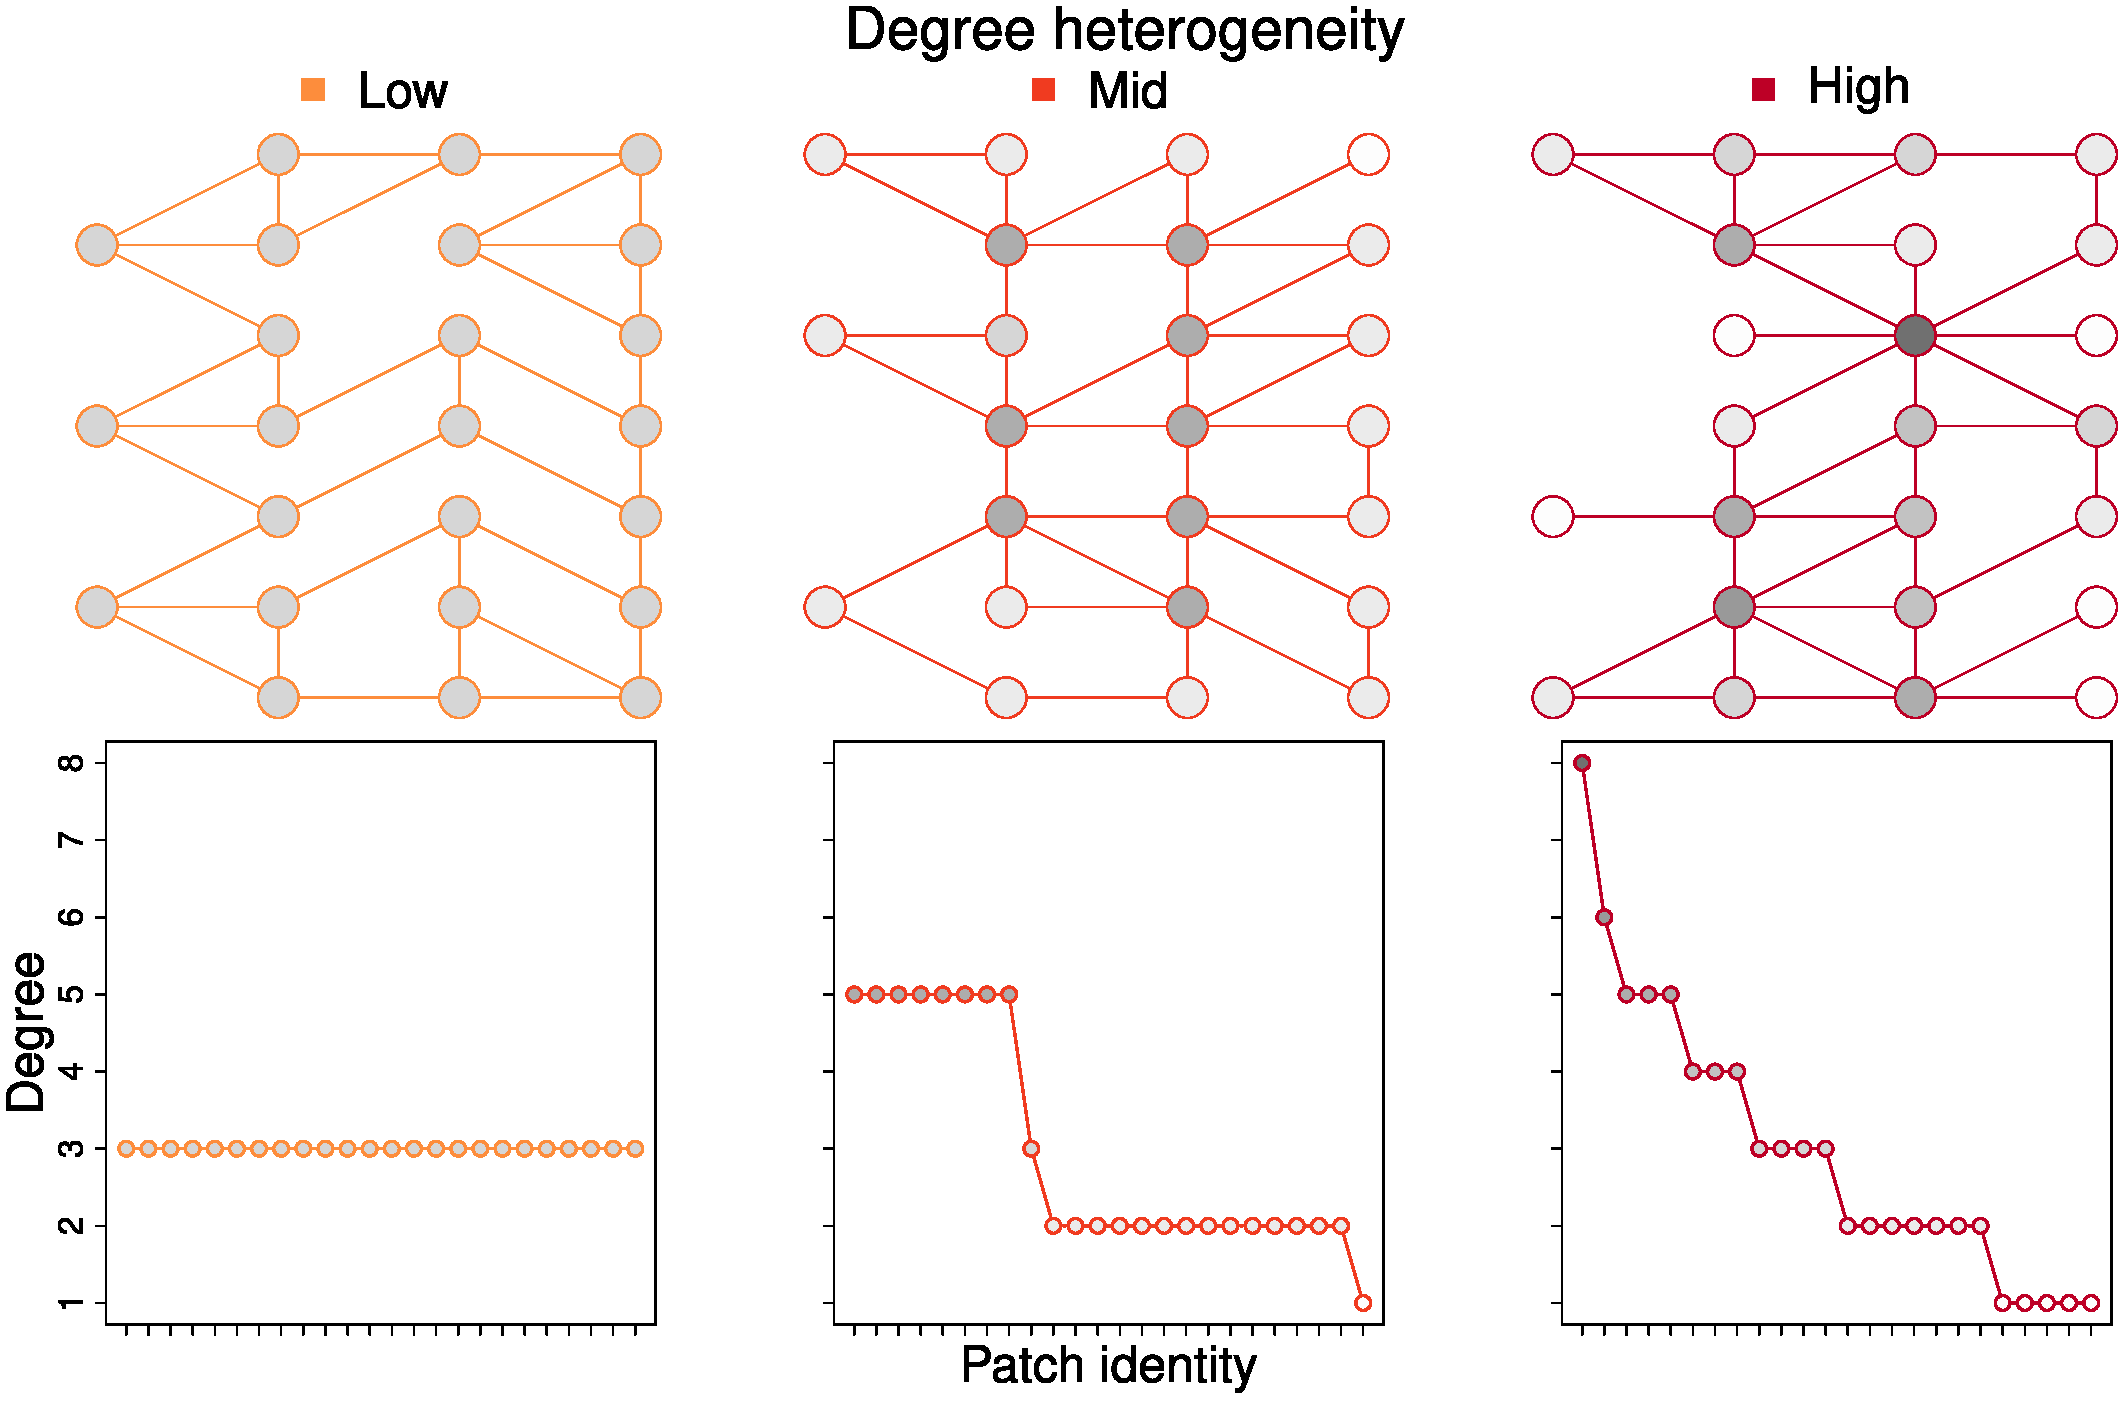
\includegraphics[width=1\textwidth]{FigSpat/concep}}
\caption[Experimental spatial networks]{Spatial networks that had different degree distribution considered in our experiment, showing a gradient of more to less homogeneous networks from left to right.} 
\label{fig:conceptual}
\end{figure}
\clearpage

\begin{figure}[ht]
\centering
\centerline{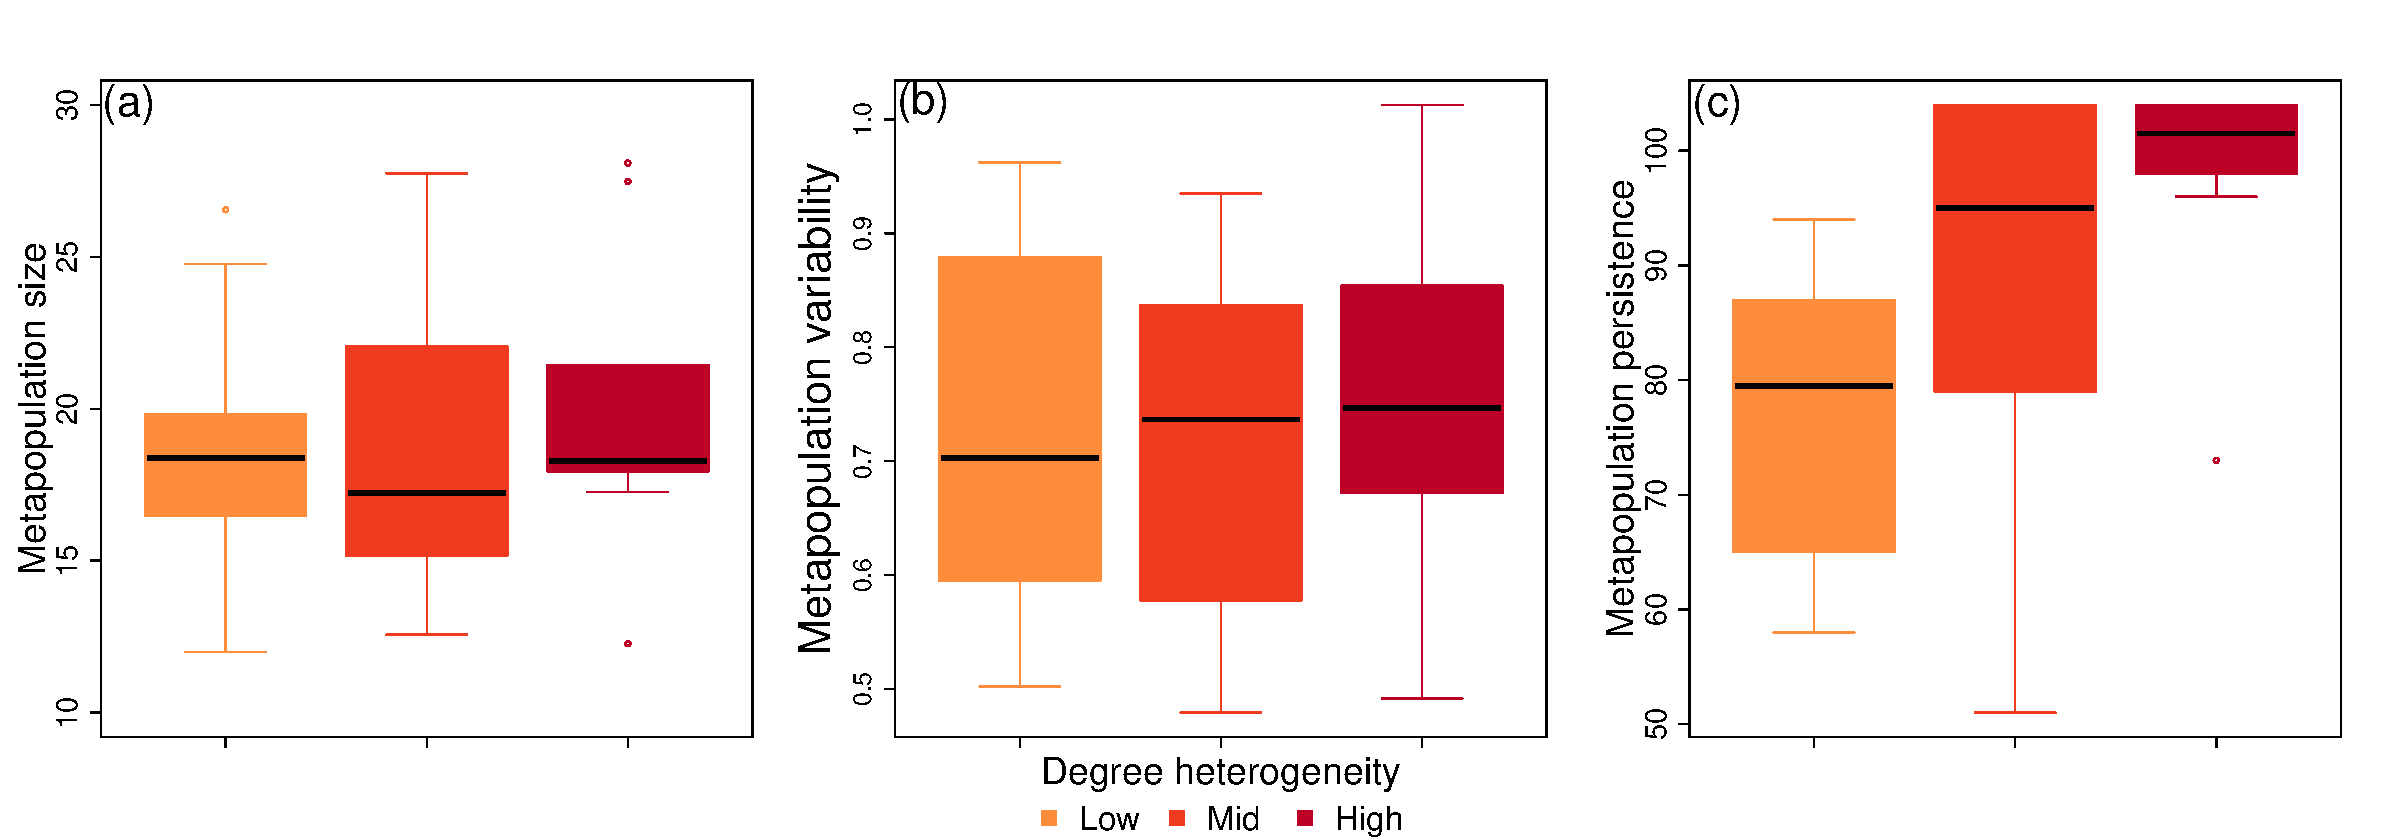
\includegraphics[width=1\textwidth]{FigSpat/meta_res}}
\caption[Effect of network type on metapopulation dynamics]{Degree distribution heterogeneity did not affect metapopulation size (a) or metapopulation variability (b), but more heterogeneous networks persisted for longer periods of time (c).} 
\label{fig:met}
\end{figure}


\begin{figure}[ht]
\centering
\centerline{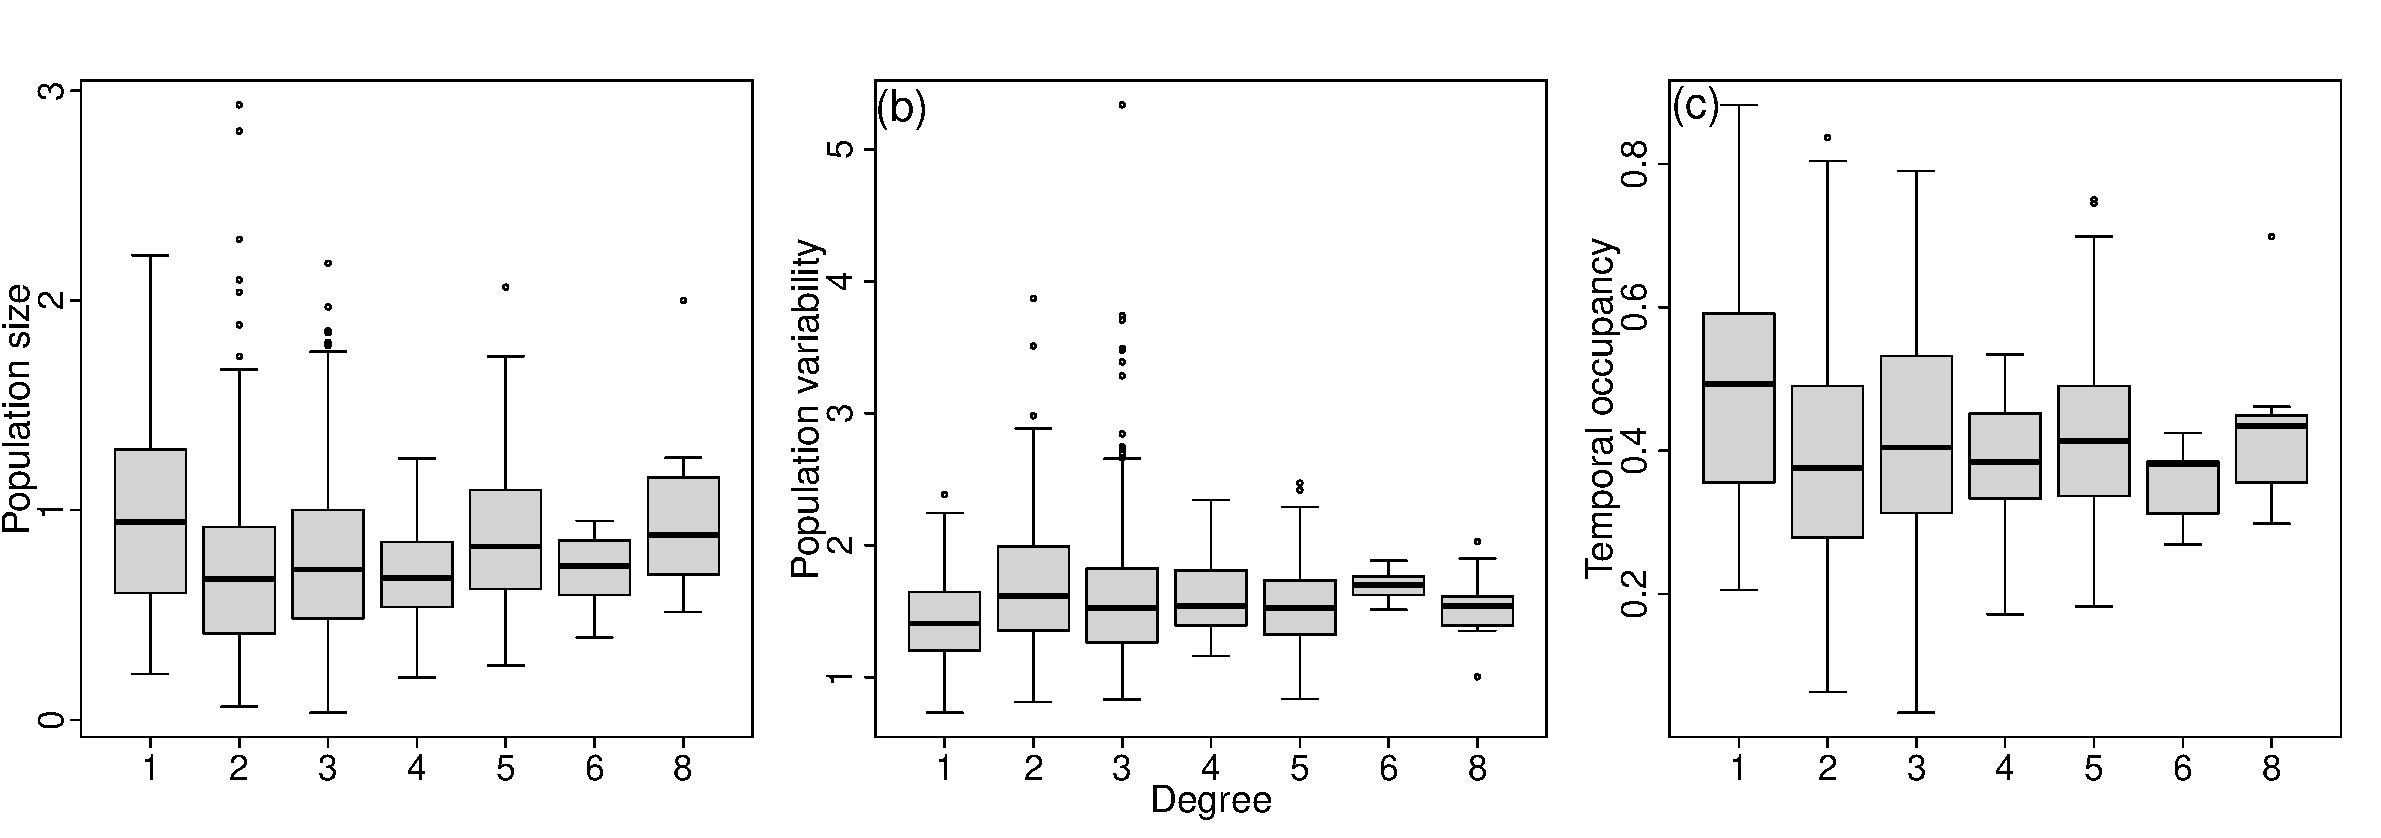
\includegraphics[width=1\textwidth]{FigSpat/pop_res}}
\caption[Effect of degree on local populations]{Degree did not affect local population size (a), local population variability (b), and the temporal occupancy of patches.} 
\label{fig:pop}
\end{figure}













                         %% Introduction.tex should begin
            
        
%\include{1mod4}            %% OF COURSE you should not use these names
%\input{flying}            %% but rather whatever is appropriate for your
%\input{joins}             %% own work!!!
%\input{wattage}

%\include{3mod4}	          %% This chapter has 8 sections
%\input{bigtime}         %% You should give your sections
%\input{smalltime}       %% logical names, rather than
%\input{roadmap}         %% numbers. As you write, you might
%\input{overview}        %% decide to rearrange things. 
%\input{turnabout}       %% LaTeX can keep track of the
%\input{fairplay}        %% numbering for you.
%\input{roundup}

%\include{rest}
%\input{relax}
%\input{grin}

%\Chaptero{References} %heading=bibintoc
%\documentclass{uscthesis}
\usepackage{graphicx}
%%%%%%%%%%%%%%%%%%%%%%%%%%%%%%%%%%%%%%%%%%
%%% Options include: [forbinding], which produces 
%%% an alternative title page and an appropriate
%%% binding margin,  [honors] for Honors College theses,
%%% and [durt] for undergraduate thesis submitted as part
%%% part of the distinction in mathematics program.
%%%%%%%%%%%%%%%%%%%%%%%%%%%%%%%%%%%%%%%%%%

%%%%%%%%%%%%%%%%%%%%%%%%%%%%%%%%%%%%%%%%%%
%%  LaTeX Preamble
%%%%%%%%%%%%%%%%%%%%%%%%%%%%%%%%%%%%%%%%%%

\usepackage[style=apa, backend=biber, uniquename=false]{biblatex}
\usepackage{graphicx} 
\usepackage{multirow}
%Packages for the review
\usepackage[most]{tcolorbox}
\usepackage{capt-of}
\usepackage{float}
%
\usepackage{footnote}
\usepackage[normalem]{ulem}
%\usepackage{hyperref}
%\bibliography{references}
%%%%%%%%%%%%%%%%%%%%%%%%%%%%%%%%%%%%%%%%%%
%% You should include above
%% any LaTeX packages that you	 need.  Most packages should work 
%% with this documentclass.
%%%%%%%%%%%%%%%%%%%%%%%%%%%%%%%%%%%%%%%%%f

\usepackage[style=uscauthoryear]{biblatex}
\addbibresource{references.bib}


%%%%%%%%%%%%%%%%%%%%%%%%%%%%%%%%%%%%%%%%
%% The lines above specify a BibTeX style which controls 
%% the appearance of the bibliography and how citations to
%% the bibliography within the text will work.  It is based on the biblatex.sty
%% package and provides a Chicago style, as preferred by the Graduate School.
%% There are other acceptable styles.  Indeed, different academic disciplines
%% have different styles.
%% 
%% The line  \bibliography{references} will cause LaTeX is search for a file
%% called references.bib.  This file could be named differently.  For example
%% \bibliography{henry} would provoke a search for henry.bib.  The
%% file reference.bib (or henry.bib) is one you will have to produce.  It is
%% a BibTeX database of references you use.
%% 
%% There are a number of alternate ways to address your bibliographic needs.
%% See the documentation uscthesisdoc.pdf  for a discussion of the different options.
%%
%%
%% 
%%In any case, this  is a good spot to ask LaTeX to load what it needs to handle
%% literature citations and to layout the bibliography. 
%%
%%%%%%%%%%%%%%%%%%%%%%%%%%%%%%%%%%%%%%%%%%


%%%%%%%%%%%%%%%%%%%%%%%%%%%%%%%%%%%%%%%%%%%%%%%%%%%%%%
%%             The Front Matter
%%  The section below deals with the material that comes 
%%  before the actual content of the document: The title 
%%  page, abstract, acknowledgments,etc.
%%
%%  Some of it is required.
%%%%%%%%%%%%%%%%%%%%%%%%%%%%%%%%%%%%%%%%%%%%%%%%%%%%%%

\title{Some Stuff about Species Interaction Networks}

\author{Grant Thomas}{Foster}    %% First Name then 
                                 %% Last Name

\degreedate{2026}                      %% The year of graduation

%\month{December}                 %% Only for the honors option
                                 %% where it is REQUIRED
\otherdegrees{
Bachelor of Science; Ecology, Biology\\
University of Georgia 2020\\ %% The \\ on this line is 
}                                %% ESSENTIAL!

\degreename{Doctor of Philosophy}     %% The Graduate School provides 
                                 %% a list of official degrees.
\field{Biological Sciences}              %% Fields also provided by the 
                                 %% Graduate School.
\college{College of Arts and Sciences}  %%As listed by Grad School

\advisor {Dr.}{Tad A}{Dallas}  %%% Be sure the 
\readera{Dr.}{Carol}{Boggs}     %%% third field is 
\readerb{Dr.}{Eric}{Lo Presti}          %%% the one used in 
\readerc{Dr.}{Melissa}{Nolan} %%% your department.
\readerd{Dr.}{Bret}{Elderd}               %%% Only use as many as
%%% If you have just two readers, for example, leave out \readerc and
%%% \readerd
%%%
%%% For Honors College theses use \reader{}{}   NO third field.
%%% The commands \otherdegrees, \degree, \field, \college, \readera, etc.
%%% are not used under the honors option.
%%%%%%%%%%%%%%%%%%%%%%%%%%%%%%%%%%%%%%%%%%%%%%%%%%%%%%%

\dean{Plato}{Founder of the Academy}   %% The Dean of the Graduate School
                   %% BE SURE TO CHECK THE NAME OF THE
                   %%PERSON CURRENTLY HOLDING THIS POSITION	
		   %% and the correct title.		             		
                     %% For Honors College theses use
                     %% \schcsigner{}{}.  For example,
                     %% \schcsigner{Dr.}{Davis Baird}

\copyrightpage       %% This is optional. It makes a 
                     %% copyright page that will appear 
                     %% immediately after the title page.

\abstract{abstract}  %% This calls the file herkimer.tex but 
                     %% but you might replace herkimer by 
                     %% anything you like, for example by 
                     %% abstract. Note, the Graduate School
                     %% REQUIRES that PhD dissertations have 
                     %% abstracts.
                     %%
                     %% For Honors College theses use
                     %% \honorsabstract{}

%\summary{precis}     %% This command calls  precis.tex
                     %% It is only available with the honors
                     %% option and it is REQUIRED for Honors
                     %% theses. 

%\acknowledgments{thanks} %% This calls the file thanks.tex 
%% This is optional       %% where you have put your 
                          %%acknowledgments.

%\dedication{dedication}   %% Calls dedication.tex
%%% Also optional

%\preface{forward}    %% Calls forward.tex.  Optional.

\makeLoT               %% Issue this command if your work has 
                       %% four or more tables.  A list of tables 
                       %% will be produced automatically.

\makeLoF               %% works the same way but for figures.

%%%%%%%%%%%%%%%%%%%%%%%%%%%%%%%%%%%%%%%%%%%%%%%%%%%%%%%%%%%%
%%  Finally, here is the meat.  The idea is to compose a 
%%  .tex file for each section of your thesis or dissertation.  
%%  Then use LaTeX's \include command to put them all together.  
%%  Doing it this way makes it easier to change the order of 
%%  exposition as your writing is in progress.  Also it
%%  makes it easy to print out just one section. The \include
%%  command always starts a new page. So every section would 
%%  start on a new page.  If you would like for sections just
%%  to continue, after the appropriate vertical space, on the
%%  current page, then use the \input command instead of the 
%%  \include command.
%%%%%%%%%%%%%%%%%%%%%%%%%%%%%%%%%%%%%%%%%%%%%%%%%%%%%%%%%%%%

\begin{document}
\chapter{Brief introduction}    %% Calls Introduction.tex
\paragraph*{} Species interactions structure ecological communities, but predicting when interactions occur and how interactions scale up to community-level outcomes remain central challenges in ecology. Natural systems are characterized by a diverse set of interacting organisms \parencite{Janzen1974Deflowering}; organizing these interaction sets into ecological networks can help us gain insight by linking pairwise interactions to community- and ecosystem-level processes \parencite{lever2014sudden, rohr2014structural}. In the framework of interspecific interaction networks, individual species represent nodes, while the interactions between species represent links. Network approaches have furthered our understanding of a variety of systems reliant on interspecific interactions, including consumer-resource, host-parasite, and mutualistic interactions, and network perspectives have yielded insights on features as specific as the dynamics of singular focal species all the way up to broad-scale patterns of community assembly and stability \parencite{guimaraes2020structure, saravia2022ecological}.

\paragraph*{} One reason network approaches are useful is that they provide a set of descriptive and mathematical tools for characterizing the architecture of species interactions. At the level of individual species, node-level properties can describe the number of interactions a species participates in (degree), the total weight of those interactions (strength), or the position of a species relative to the rest of the network. Centrality, for example, describes how connected a species is to other members of a network and is often used to identify species whose loss may have disproportionate effects on associated communities \parencite{traveset2017plant, maia2019plant, martins2024propagation}. Understanding the ecological and evolutionary processes that give rise to variation in node-level properties is therefore important for understanding how interaction networks are organized and how they may respond to disturbance \parencite{moulatlet2023species, martins2025determinants, zhang2025network}.

\paragraph*{} In addition to node-level characterizations, network approaches can also summarize the overlying architecture of species interactions within a community. Network-level properties include summaries of how links are distributed among species, such as degree distributions and connectance, as well as properties describing the arrangement of links, such as modularity and nestedness \parencite{bascompte2003nested, bascompte2006asymmetric}. These structural properties are of interest because they can influence emergent features of ecological systems, including stability, resilience, robustness to species loss, and the propagation of perturbations through communities \parencite{thebault2010stability, suweis2013emergence, bascompte2022resilience, martins2024propagation}. As a result, understanding the factors that shape network structure can provide insight into both the assembly of ecological communities and the potential responses of those communities to environmental change.

\paragraph*{} The architecture of species interactions emerges from processes operating across multiple scales. Species-level traits \parencite{rafferty2013, ramos2018fruit}, phylogenetic relationships \parencite{eriksson2016evolution}, geographic distributions \parencite{moulatlet2023species}, environmental tolerances \parencite{slatyer2013niche}, local community composition \parencite{saravia2022ecological}, biogeographic context \parencite{sugiura2010, dalsgaard2013, traveset2016, nogales2024review}, and anthropogenic impacts \parencite{teixido2022anthropogenic, cruz2023mutualisms, birkenbach2024land} can all influence which interactions occur and how they are organized. However, the relationship between these factors and interaction structure is not always straightforward. Processes that shape species assemblages may not translate directly into the structure of interactions among those species, and the meaning of network properties may shift between local communities, regional metawebs, and broader macroecological contexts. In this dissertation, I examine how interspecific interactions are organized across these scales in mutualistic, antagonistic, and competitive systems.

\paragraph*{} Like any data collection process, the sampling of ecological networks is imperfect. Even intensive sampling may fail to capture rare interactions or, in some cases, rare interactors \parencite{Young21}. Because biased errors in network construction can alter inferred network structure, incomplete sampling creates challenges for understanding how interactions are organized \parencite{bluthgen2008, Young21}. In chapter two, I address this problem by comparing random-forest regression models informed by combinations of phylogenetic structure, species traits, and latent network structure in their ability to fill in potentially missing interactions in a diverse network of fruiting plants and frugivorous birds in Brazil's Atlantic forest. This chapter highlights the potential importance of latent structural features for predicting mutualistic interactions, and encourages a clear conceptual link between prediction performance metrics and the overall goal of predicting cryptic links.

\paragraph*{} Species’ roles within interaction networks may also depend on processes operating across spatial scales. Highly central species may have disproportionate effects on their associated communities \parencite{traveset2017plant, maia2019plant, martins2024propagation}, but the factors contributing to species' position within interaction networks may differ across biogeographic scales. Identifying the eco-evolutionary processes that give rise to highly central species in local and regional-scale interaction networks is essential for understanding how ecological networks are organized and how they may respond to disturbances \parencite{moulatlet2023species, martins2025determinants, zhang2025network}. In chapter three, I combine a globally distributed dataset of floral visitation networks comprising 30,330 interactions among 6,857 species with large-scale occurrence data to evaluate how species’ geographic and environmental range sizes impact their role in networks across scales. These results suggest that the apparent impacts of geographic range size on species centrality in large-scale metawebs are primarily driven by interaction turnover and the scaling of interaction specificity from local to global networks. When variation in interaction turnover is incorporated, niche breadth exerts the strongest positive effect on plant centrality within both local and global floral visitation networks. 


\paragraph*{} The structure of species interaction networks is shaped by both biotic and abiotic contexts, and the increasing availability of ecological data has permitted examinations into how spatial and environmental gradients influence the structure of these species interaction networks \parencite{tylianakis2017}. In chapter four, I take a macroecological approach to investigate how bipartite interaction networks between free-living hosts and helminth parasites vary across gradients of island area and isolation. I find that relationships between island characteristics and the species richness of both hosts and helminth parasites are broadly consistent with predictions from classical island biogeography theory for free-living species. In contrast, network nestedness showed a more limited response, increasing weakly with island area while failing to respond to either measure of island connectivity. These results suggest that island characteristics shape the richness of host-parasite assemblages more predictably than the structure of interactions within them.

\paragraph*{} Global ecosystems are subject to anthropogenically driven changes at increasing rates, and as a result, so are the mutualistic interaction networks that occur within them. Structural changes in mutualistic networks can be driven by a diverse set of drivers, including shifting climates, urbanization and land use changes, and invasion of non-native species \parencite{traveset2014mutualistic, teixido2022anthropogenic, cruz2023mutualisms}. In chapter five, I characterize the current state of understanding of how these drivers affect the structural properties of two major classes of plant-animal transport mutualisms: seed dispersal and pollination networks \parencite{bronsteinmutualism1}. I also examine how knowledge of these patterns can be used to better understand, predict, and conserve these critical natural systems.

\paragraph*{} Finally, in chapter six, I investigate how species-level performance and interspecific interactions scale up to community assembly outcomes. Single-species vital rates are one possible source of simplified demographic information that may be useful in predicting community outcomes \parencite{ram2019predicting, nestor2023interactions}. Using experimental microbial communities, I test whether demographic parameters derived from monoculture growth experiments can predict multi-strain community outcomes across nutrient environments. Together, these results show that single-species growth parameters can provide useful predictions of community assembly, but that their predictive value depends on environmental contexts.

\paragraph*{} Collectively, these chapters show that the structure and consequences of interspecific interactions are shaped by processes operating across multiple scales. Species traits, phylogenetic relationships, latent network structure, geographic range size, climatic niche breadth, island biogeography, anthropogenic change, and environmental contexts can provide insight into how ecological interactions are organized, but their importance varies across systems and scales. Together, this work contributes to a multiscale view of ecological interactions in which community structure depends not only on whether species interact, but also on how species are embedded within networks, where those networks occur, and how interactions scale up to community-level outcomes.
    %% Calls Introduction.tex
                          %% Introduction.tex should begin
                          %%
                          %% \chapter{Introduction}
                          %% followed by the text of the 
                          %% introduction.
\addtocontents{toc}{\protect\vskip-20pt}                          
\chapter[Comparing the power of phylogenetic, trait, and network structure information to predict plant-frugivore interactions.]{Comparing the power of phylogenetic, trait, and network structure information to predict plant-frugivore interactions\footnote{Published as: Foster, G., \& T. Dallas. Comparing the power of phylogenetic, trait, and network structure information to predict plant-frugivore interactions. \textit{Oikos} 3, e11156. 2026. Reproduced here under the CC BY 4.0 license terms. See Appendix D.}}  
           
\section*{\textbf{\underline{Abstract}}}
%This is exactly the 200 word limit
Due to the constraints of limited effort and sampling error, observed species interaction networks are an imperfect representation of the ``true'' underlying community. Link prediction methods allow us to construct a potentially more complete representation of a given empirical network by guiding targeted sampling of predicted links, as well as offer insight into potential interactions that may occur as species' ranges shift. Various data types can predict interactions; understanding how different kinds of information compare in their ability to predict links between different types of nodes is important. To this end, we compare random-forest regression models informed by combinations of phylogenetic structure, species traits, and latent network structure in their ability to predict interactions in a diverse network of fruiting plants and frugivorous birds in Brazil's Atlantic forest. We found that for our dataset, latent structure was the most important determinant of model predictive performance. While incorporating trait or phylogenetic information alongside latent features had little effect on discriminatory power, they did meaningfully increase overall model accuracy. Our results highlight the potential importance of latent structural features for predicting mutualistic interactions, and encourage a clear conceptual link between prediction performance metrics and the overall goal of predicting cryptic links.

\section*{Introduction}
\paragraph*{}
Natural systems are characterized by a diverse set of interacting organisms; organizing these interaction sets into ecological networks can help us gain insight into community and ecosystem-level processes. Whether consumer-resource, host-parasite, or mutualistic networks, understanding which species interact and why can give us insight into features as specific as the dynamics of one focal species all the way up to broad-scale patterns of community assembly and stability \cite{guimaraes2020structure, saravia2022ecological}. As such, ecologists have put a great deal of effort into observing and quantifying the interactions found in nature. However, like any data collection process, the sampling of ecological networks is imperfect. No matter how much effort we put into characterizing a network, we may often miss observing interactions (links), or even interactors themselves (nodes) \cite{Young21}. Moreover, the likelihood of observing a given interaction is related to factors such as the abundances of both interactors \cite{canard2014empirical}, with the total interaction set of rare species less likely to be represented accurately \cite{cirtwill2019quantitative, olesen2011missing}. Errors in the construction of ecological networks, especially when biased, can lead to dramatic changes in network structure \cite{bluthgen2008, Young21}. Ecological networks are also temporally dynamic. Local species turnover can add or subtract links, while regional-scale extinctions, evolution, or range shifts may rewire existing connections \cite{olesen2011}. 

\paragraph*{}
Increasing sampling intensity or duration could solve these problems; as sampling effort increases it is less likely for rare links to go unobserved, allowing for a more accurate representation of the true network structure. However, the resources that can be devoted to sampling are limited. While the increasing availability of passive monitoring technologies\cite{quintero2022methodological}, as well efforts to extract interaction data from existing large-scale occurrence datasets \cite{putman2021power} may increase the availability on interaction data, the problem of incompletely sampling interactions will never fully disappear. A potential way to address this shortfall is to utilize predictive approaches to decide which particular species or links should be targeted for additional sampling. To this end, the goal of predicting cryptic links between nodes allows us to more productively focus limited sampling resources \cite{terry2020finding}. Predictive approaches also allow for us to predict network organization arising from novel complements of species. Identifying likely or unlikely possible linkages between invading species and already present interactors allows us to get a more complete picture of biotic constraints on invasibility \cite{minoarivelo2016invading}, and ultimately a better understanding of how species interaction networks may be altered by anthropogenic forcing.  

\paragraph*{}
Symbiotic interactions are dependent on a complex set of factors including life history \cite{ramos2018fruit}, phenotypic traits \cite{rafferty2013}, co-evolutionary history \cite{eriksson2016evolution}, spatial and temporal distributions \cite{fricke2020accelerating, menke2012plant, laurindo2020drivers}, as well other biotic interactions \cite{carreira2020question}. Incorporating information that either directly influences, or conveys information about these factors into link prediction frameworks should hopefully improve prediction performance \cite{dallas2017predicting}. When applying link prediction in practice, we often have a variety of species and interaction-level properties at our disposal, many of which may perform better or worse at predicting in certain types of networks or interactions. Understanding which types of information may be better or worse at predicting interactions in different contexts, however, is still an open avenue of research. 

\paragraph*{}
For plant-frugivore seed dispersal systems, information on node morphological and life history traits (gape-width, fruit characteristics, geographic or phenological or overlap), may be at the root of why many species do or do not interact \cite{bender2018morphological,gonzalez2015relative, moran2010can}. Trait matching link prediction approaches are able to use suites of continuous or discrete traits that either directly or indirectly influence interaction probability across a large number of species. These approaches perform well in situations when a small number of traits are linked to interaction probabilities across many species (eg. flower and beak morphometric traits in flower-hummingbird pollinator systems \cite{pichler2020}. However, while trait data may give us insight into biological underpinnings of network connections we observe, they may not always be the most appropriate for link prediction methods. Interactions may be determined by a large suite of traits that individually contribute small amounts. Alternatively, traits relevant for one taxonomic group may not be relevant for another (gape size may be predictive for birds, but not for primates). Or interaction propensities may be controlled by traits difficult to quantify, such as microhabitat usage or foraging strategies. In all of these cases, trait-matching approaches may perform relatively poorly for some or all types of nodes in a given network. In these cases, alternative information sources such as phylogenetic information or latent network structure may be useful for link prediction. 

\paragraph*{}
Using phylogenetic relationships between species may be useful for predicting links due to a number of factors. Firstly, traits that mediate species interactions may be phylogenetically conserved, allowing us to treat information about phylogenetic relationships between organisms as a proxy for traits. This assumption may be especially useful when traits governing interactions are numerous, hard to measure, or hard to identify. However, phylogenetic conservatism may break down at fine evolutionary scales, making phylogenetic information an imperfect proxy for traits governing interactions \cite{rafferty2013}. Additionally, while post-hoc correlative investigation may be able to suggest potential traits of interest, this approach ultimately further abstracts from the mechanisms governing interactions even if prediction performance is quite good. Despite these shortcomings, in the use-case of targeting potential links for surveillance (in essence a prediction problem), a phylogenetic approach may still be quite useful. In addition to proxying traits, as coevolutionary history between organisms can often be an important factor governing the presence of an interaction, incorporating phylogenetic information may be vital to represent this linkage. While plant-frugivore networks may in generally be less coevolutionarily linked and more asymmetric some other classes of ecological networks\cite{maglianesi2024phylogenetic, jordano1987patterns, wheelwright1982seed}, capturing nodes' shared evolutionary history may still be important for prediction. By definition phylogenetic methods require a phylogeny that includes all the species you intend to predict interactions for, causing potential limitations for predicting in systems where phylogenetic information may be incomplete. However, as the cost and time required to sequence non-model genomes has and continues to decline, the problem of data availability continues to become a more and more surmountable barrier to prediction. To-date, phylogeny-based interaction predictions have been successfully implemented in a number of mutualistic network systems, including plant-pollinator interactions \cite{Braga21}.



\paragraph*{}
Independent of the phylogenetic relationships and traits of individual nodes in a network, latent structural features of networks themselves may actually be useful for predicting missing links. In this context, the term ``latent features" refers broadly to properties derived from the structure of the interaction network through any number of dimensionality-reduction approaches \cite{poisot2021imputing}. While there are a multitude of different methods used to create latent network features for interaction prediction (single-value decomposition, random dot product graphs \cite{strydom2022food}, graph motif distributions, matrix factorization \cite{seo2018predicting}, etc), we focus on single-value decomposition, an eigendecomposition approach already used with some success in describing the structure of and assisting in the prediction of empirical foodwebs \cite{banville2023constrains} and host-virus associations \cite{poisot2021imputing, poisot2023network}. Once an existing network is known, calculating latent structural features is computationally tractable. While arguably even more agnostic to the mechanisms driving species interactions, this structural information may capture particular types of real linkages difficult to discover based on trait or phylogenetic information alone. 


\paragraph*{}
Prevailing interaction prediction approaches have often centered on a single information type, but recent work in host-parasite systems have emphasized the power of machine learning approaches to synthesize multiple data types to predict interactions \cite{strydom2021roadmap}. Despite the use of this variety of information streams for link prediction problems already, studies directly comparing the predictive capacity of phylogenetic, trait, and latent features are few, and have not been applied in plant-frugivore systems. Beyond looking at the performance of these feature classes independently however, knowing how they may be used together is another important avenue of research. By looking at the performance of models trained on combinations of different data types are better able to understand whether different methods overlap in the types of links they predict well, and perhaps more importantly whether we can use these information streams in concert to create models that are more than the sum of their parts. To this end, we apply random forest prediction algorithms to predict plant-frugivore interactions in Atlantic forests in Brazil using combinations species trait data, phylogenetic information, and latent structural features. 

\section*{Methods}

\paragraph{Trait and Interaction Data}
The full interaction network is published by Bello et al. \cite{bello2017}, and includes a total of $5,226$ unique species interactions between $787$ and $342$ plant and frugivore species, respectively. Due to the availability of phylogenetic and trait data, we restricted our analyses to avian-plant interactions, representing the most species-rich set of frugivores in this dataset ($3,856$ unique interactions between $394$ and $242$ plant and bird species, respectively). Of our avian-frugivore species (hereafter frugivores), numbers of unique plant interactions per frugivore ranged from 1 (53 species) to 120 unique plant interactions recorded for \emph{Turdus rufiventris}; median frugivore degree was 5. The number of unique frugivore interactions per plant was generally lower, ranging from 1 (128 species) to 80 unique frugivore interactions recorded for \emph{Myrsine coriacea}; median plant degree was 2. Overall this interaction network is characterized by a relatively high degree of phylogenetic generalism. Out of 187 frugivore species that interacted with more than one plant for which phylogenetic information is available, only 9 interacted with a group of plants more phylogenetically related than random chance (\cite{kembel2010picante}, see supplement\ref{supplement}). 

\paragraph*{}
The Bello et al. dataset includes a number of informative traits for both plant and frugivore nodes. Frugivore traits include allometric measures such as body mass and gape size, life history traits such as degree of frugivory and migratory status, and population traits such as  IUCN listing and population trends. Frugivore mean body mass was unavailable for 3 species, while mean gape size was unavailable for 68 species. Plant traits include fruit mass, seed diameter fruit color, growth form, fruit lipid concentration (scored 1-3), IUCN listing, and whether it is a native or nonnative species. For trait-based models, species were filtered to only include those with complete sets of trait data (174/242 frugivore species). As part of our research goal was to compare the power of phylogenetic and trait data, we chose to omit these species for trait based models rather than phylogenetically impute missing trait information. Categorical variables (such as plant growth form) were transformed into a series of binary variables through one-hot encoding. Continuous data on fruit size was available for 280/394 plant species; plants without trait data were again excluded from trait-based models. Details on plant and frugivore traits used in the analysis are available in Table \ref{tab:traits}). 
    


\paragraph{Phylogenetic Data}
For plant species, phylogenetic data was retrieved from the BIEN database, accessed using the r package `BIEN` \cite{maitner2018bien}. Out of 787 plant species in our dataset, 646 occurred in the BIEN phylogeny. 61 plant species with a recorded avian frugivore interaction did not occur in this phylogeny. For absent species with a congeneric in our phylogeny, we added those species as a polytomy at the parent node of that genera, allowing us to add an additional 46 species to our analysis. 16 species did not have congenerics present in the network, and were discarded from the analysis. Results were qualitatively the same if these polytomies are omitted from the analysis (see supplement). Bird phylogenies were retrieved from VertLife \cite{jetz2012}; for our analysis, we used 100 trees sampled from the Bayesian posterior distribution. Phylogenetic information was unavailable for two bird species in our network. As with plants, both species were added as polytomies at their respect parent genera. Each sampled tree was used in one of one hundred replicates for each model incorporating phylogenetic data. For both the plant and bird phylogenies we performed eigenvalue decomposition, and trained phylogenetic models on the first 4 dominant eigenvectors for plants and the first 3 dominant eigenvectors for birds. The incorporated eigenvectors explained 37.2\% of variation for plants. While the exact amount of variation explained by the incorporated eigenvectors differed among sampled trees for birds due to variation in posterior samples, on average the incorporated eigenvectors explained $46.02\pm 2.29\%$ of variation for birds. 


\paragraph{Latent Methods} We used single-value decomposition (SVD) of the full interaction matrix to create continuous latent features to be used for prediction using the `SVD()` function in base R \cite{RCore}. We used the first three axis of variation for both plants and birds as continuous predictors. Due to the incompatibility of latent network features with out of sample prediction, during model validation we derived node-level latent properties form the full interaction network, though each training set utilized only a portion of these nodes. 


\paragraph{Model Structure and Comparison} We used random forest regression models informed by different feature types to make comparisons across types of information, as implemented in the R \texttt{randomForest} package \cite{randomForest}. We tested a total of 7 models; three using predictors from only one type of information (traits, phylogeny, or latent features), three pairwise combinations of each predictor class, and one model incorporating all possible predictors. In order to validate model performance, we trained 100 iterations of each model. Like most empirically observed ecological networks, our training network was very sparse\cite{vazquez2009uniting}. Our total potential interactions matrix included 3,643 observed interactions and 90,917 unobserved interactions. To address this class imbalance, for each iterations we first randomly selected 80\% of our data for training, and then randomly removed unobserved interactions from the edgelist (i.e. rows of the edgelist where the interaction value is equal to 0) from the training data until we achieved a 1:3 ratio of observed:unobserved interactions. After model training, performance was evaluated on the remaining 20\% test set. We analyze model performance both through area under the receiver-operator curve (AUC), which measures model discriminator power, and mean root squared error (RMSE), which measures prediction accuracy. These two measures are commonly used to evaluate the effectiveness of predictive approaches \cite{norberg2019comprehensive}, but the choice of which metric to optimize may be different depending on the use case in question (see discussion). For each model iteration we also recorded the optimal suitability threshold for classification as the value that maximized Youden's $J$ \cite{youden1950index}.


\paragraph{}
After validating model predictive performance using this test-train split, we then re-ran 100 iterations of each model using the full network without internal class balancing. Using the full suite of interaction information allows us to better predict potential unobserved links. We present the pairwise suitability correlations of each of these full model outputs, as well as present a list of links predicted to be highly suitable by one or more of our models but that are not observed to occur in this data set. We then used the average optimal threshold value for each model as model-specific thresholds for classification. For each model, variable importance was quantified by mean decrease in Gini coefficient  (MDG) after permutation of each variable as implemented in the R \texttt{randomForest} package \cite{randomForest}. A common variable importance metric for classification problems, MDG is calculated by normalizing the sum of all decreases node impurity by the total amount of decision trees in the ensemble \cite{khalilia2011predicting, calle2011stability}. A higher MDG value for a given variable indicates that variable is more important to model performance. 






\section*{Results}

\subsection*{Model Performance}
Using an 80-20 split of testing and training data, all models were able to predict testing interactions with reasonable accuracy and discriminatory power (Figure \ref{fig:Figure_1}). AUC was lowest for trait only models (0.84 $\pm.009$) followed by phylogeny only models (0.85 $\pm .009$). All models including latent information outperformed latent-agnostic models in terms of discriminatory power, with the greatest AUC achieved by Latent (0.94 $\pm .004$) and phylogeny-latent models (0.94 $\pm .004$), both of which even outperformed the full trio model (0.93 $\pm .006$). However, prediction accuracy did not follow the same trends as discriminatory power. Latent and trait-only models had the lowest overall accuracy (56.0, $\pm 0.32$ amd $\pm 0.40$, respectively), while the most accurate models were those combining trait information with another information type. The trio model was the most accurate (RMSE: 48.6 $\pm .37$), closely followed by the trait-phylogeny (RMSE: 49.2 $\pm .36$) and trait-latent models (RMSE: 49.0 $\pm .37$). The trait-only model had only middling accuracy performance however (RMSE: 52.8 $\pm .57$).

    
\subsection*{Variable Importance on Entire Network}
After validating model performance on novel test-data, we then retrain replicate models of each type on the full network in order to generate more robust predictions. Variable importance was quantified by mean decrease in Gini coefficient after permutation of each variable. In all models incorporating them, latent SVD features were unilaterally the most important variables for prediction (Figure \ref{fig:Figure_2}); all models latent models ranked plant SVD axis 1 as the most important followed by frugivore SVD axis 1, with some variation as the ordering of the rest of the SVD axis importance. For the trio model, frugivore mass and fruit diameter were the next to important traits, which was consistent with the ordering of all other trait models. While the next most important trait was frugivore gape size for the trio model, for other models incorporating trait information fruit length was the next most important trait. 

\paragraph*{}
In general, we found that continuous frugivore traits (body mass, gape width) were more informative to prediction than continuous plant traits. Similarly, phylogenetic information about frugivores was generally more important for prediction than phylogenetic information for plants. In the phylogenetic-only model, all three frugivore phylogenetic eigenvectors were more important than all plant eigenvectors, while for the trio model only plant eigenvalue axis 2 was more important than frugivore eigenvalue axis 2. Out of the remaining traits, the trio model was most informed by frugivory level, with the the remaining categorical plant traits impacting Gini coefficient very little for all models. 



\subsection*{Comparing models}
Across the entire network, suitability values between all models were highly correlated (Figure \ref{fig:Figure_3}); most models were able to correctly discriminate between observed and unobserved links. While the ability to reconstitute observed links is important for model performance, focusing on model agreement on suitability of unobserved interactions can provide insight into which models may identify different potential interactions. Across all potential links, Spearman's rank correlation of predicted suitability values showed low correlation between phylogenetic and trait models ($\rho = 0.643$), despite both exhibiting very similar overall performance. Phylogenetic and latent models showed the lowest agreement in suitability predictions of all pairwise combinations of models, with $\rho = 0.566$ when comparing across all links, which then dropped to $\rho = 0.032$ when only looking at unobserved links. This marked drop suggest that suggests an that most agreement between suitability ranking between these models was in known interactions. The low agreement between the ranking of potential interactions pose a barrier to meaningfully target potential sampling based on the results of these two models used independently.

\paragraph*{}
Similarly, suitabilty predictions of composite and individual component models tended to mirror relative information type importance. For example, suitability values from trait-latent model were more tightly correlated with those from the latent model ($\rho=0.882$) than the trait model ($\rho=0.773$). Table \ref{tab:confusion} presents the confusion matrix for all models after classifying points according to each models' average optimal threshold value across all training iterations. We see that at their optimal threshold value, all models exhibit markedly low false-negative rates with the exception of the trait only model, which exhibited a false-negative rate of $4.80\%$.








\section*{Discussion}
\paragraph*{}
Models incorporating latent structural features consistently outperformed models that excluded them in terms of discriminatory power, but had generally lower accuracy. In contrast, trait based and phylogenetic models displayed lower AUC values, but better a better RMSE. Overall performance of phylogenetic and trait-only models were remarkable similar in terms of both performance measures used. Incorporating latent features into each model once again yielded nearly identical discriminatory  capacity, but an overall slightly higher accuracy for the trait-latent features model compared to the phylogeny-latent feature model. The discriminatory power of each individual model generally reflects the relative importance of variable information types \ref{fig:Figure_2}. 

\paragraph*{}
The strength of latent features for prediction may stem from the fact that latent features are particularly suited to predicting interactions in relatively generalist interaction networks. Frugivorous vertebrates often tend to exhibit a high average degree of generalism \cite{richardson2000plant}. In systems characterized by low interaction specificity, latent features may be more efficient at capturing neutral processes that may be underlying community assembly processes. Especially abundant, wide-ranging, or generalist hosts may contribute to a "rich get richer" effect, where hyper-generalists that already interact with many species likely interact with even more partners. Host abundance in particular has been shown to be an important determinant of interaction probability in other neotropical frugivory networks \cite{laurindo2020drivers}. Latent features, such as those created through network dimensionality reduction or motif completion, may perform particularly well in generalist interaction networks. 

\paragraph*{} 
While comparing models in terms of discriminatory power highlights the importance of latent features, incorporating phylogenetic or trait information alongside latent features actually improves model accuracy measures (RMSE), despite slightly reducing discriminatory power. The question whether it is better to optimize one metric or the other, is largely dependent on the particular use case. As we've presented the problem of link prediction, primarily as a way to guide sampling efforts to more efficiently measure networks on limited resource, discriminatory power is likely a more apt metric. Beyond ranking different links, the relative confidence in each link is of less concern as the most likely links will be validated with additional observation data. However, if your task was something closer to filling in a partially sampled network and then analyzing its properties, a metric like RMSE or H-measure\cite{hand2009measuring} may be more appropriate as it better allows you to directly incorporate uncertainty about particular into your resultant analyses. 


\paragraph*{} In models incorporating frugivore and plant phylogenitic information, the frugivore phylogeny tended to be more important to model performance. Ideally, this is likely because patterns of interactions are more phylogenetically conserved between frugivores than plants. This may be due to the frugivore phylogeny being more full summarized by a smaller number of eigenvectors. On average, the first three eigenvectors of the decomposed frugivore phylogeny explained $46.02\%$ of total variation across the phylogeny on average, while the first four eigenvectors only explained 37.5\% of variation for plants.% Including only the first three plant eigenvalues further decreased model performance \ref{add supplement}. 
The difference in variation and resultant effects on prediction may be due to overall structural features of the phylogeny, or differences in the total phylogenetic divergence characterized by the tree.

\paragraph*{} Our modeling approach represents a useful framework for predicting species interactions in a variety of systems, but care must be taken when interpreting the results in the particular context of each system. While we ultimately find that latent features dominate prediction in our system, the potential for information leakage between test and train sets means we must be conservative in our interpretation of comparisons across models. Due to the nature of matrix decomposition approaches, neither latent features nor phylogenetic information can be used to predict out of bounds. The decompositions must be performed on the entire network before performing the test-train split, potentially leading to information leakage. However, this phenomenon is only a potential problem when comparing performances on subdivided training data, and should not affect our predictions using the entire network. The dominance of latent features using internal cross-validation metrics support their importance in our system. Despite their caveats, latent features have already been successfully implemented to predict links in a variety of ecological network types, and can provide significant improvements in predictive performance in a variety of contexts.\cite{banville2023constrains, poisot2021imputing, poisot2023network, nunes2024estimated} Future work investigating the utility of latent features to predict frugivorous interactions in a variety of empirical systems and the mechanisms through which they act represents an important avenue for future research.  Similarly, our presented interpretations of the effect of phylogenetic information on prediction to their ability assume they at least partially capture phylogenetically conserved traits  or aspects of shared evolutionary history. However, while phylogenetic relationships do impact at least some of the species traits governing interactions, there may be other confounding information (such as a phylogenetic  biases of studiedness) within phylogenetic information as well. While not reducing overall link prediction performance, this does mean we should once again take a more conservative interpretation of our prediction results when comparing across models, as is the case with any correlative approach. 

\paragraph*{}
Link prediction is a promising method to deal with the realities of incompletely sampled natural systems, and may play an increasingly important role in helping to gain insight into how interactions networks may change over time. Anthropogenic effects on climate, landcover, and biodiversity all have the potential to fundamentally alter mutualistic networks, whether through changing mutualistic assemblages themselves, or the probability of interactions within a network \cite{tylianakis2017ecological, memmott2007global, teixido2022anthropogenic}. Positive feedbacks within mutualistic communities may often make them more likely to exhibit alternative stable states, and changes in mutualistic communities may result in drastic changes to network structure and resulting assemblages \cite{lever2014sudden, bascompte2022resilience}. Link prediction methods provide an opportunity for us to better understand which species are interacting now, and which may interact in the future. Prediction approaches can also be useful when predicting the potential effects of invaders on mutualistic network structure \cite{fricke2020accelerating,traveset2014mutualistic}. To fully understand and predict the scope of mutualistic network change, future work applying predictive approaches to temporally sampled mutualistic networks is necessary. Understanding the spatial and temporal scales at which mutualistic interactions turn over or change strength is a vital next step for understanding the dynamics of mutualistic networks in a changing world.\\

\noindent \textbf{Acknowledgements}: This work has been performed with funding to both authors provided by ANONYMIZED. 

\noindent \textbf{Open Research statement}: All $R$ code and data necessary to reproduce this is available on figshare at \\ \texttt{https://figshare.com/s/544021fc48732ca5bb13}.


\clearpage
%\bibliographystyle{rss}
%\bibliography{Fruglink}

\clearpage 

\section*{Tables} 


\begin{table}[!h]
\caption{Frugivore and plant traits used for interaction prediction. Non-ordinal factors such as fruit color were transformed through one-hot encoding prior to inclusion in the model.}
\label{tab:traits}
\begin{tabular}{clll} 
 \hline
 Species & Trait & Units & Range/Levels \\  
 \hline
 \hline
Frugivore & Body Size &  g &  6.60 - 3500 \\
& Gape Size &   mm  & 2.80-36.29  \\  
& Degree of Frugivory & factor   &  low, medium, high \\  
Plant & Fruit Diameter &  mm  & 1.2-325  \\
& Fruit Length &  mm  &  1-600 \\
& Fruit Color &  mm  & yellow, red, black, brown, green, other \\
& Fruit Lipid Content & factor   &  low, medium, high  \\ 
& Plant Growth Form &   factor  &  tree, liana, palm, scrub, other \\ 
 \hline
\end{tabular}
\end{table}


\clearpage 


\begin{table}[]
\caption{True and false positive and negative rates for models trained on the entire interaction network, classified assuming the average threshold value across all training interactions that maximized Youden's $J$ statistic. Percentages represent proportions in each category out of all total links each model predicted; the absolute count of each category is represented in parenthesis. Total number of predicted links differed across models according to availability of covariant data.}
\label{tab:confusion}
\begin{tabular}{@{}lllll@{}}
\toprule
%{\ul } & {\ul } & {\ul } & {\ul } & {\ul } \\ 
   \textbf{Model}    &  \textbf{True Positives}      &    \textbf{False Positives}    &    \textbf{True Negatives}    &    \textbf{False Negatives}    \\
\midrule
\textbf{Latent}   &  3.85\% (3,643)      &    0.28\% (263)&    95.87\% (90,654)&    0.00\% (0)    \\
\textbf{Phy}       &   3.87\% (3,350)&  0.27\% (231)&   95.66\% (82,806)&     0.29\% (175)\\
\textbf{Traits}       &   1.86 \% (778)&  0.22\% (92)&  93.20\% (39,021)&       4.73\% (1,979)\\ 
\textbf{PhyLatent}       &    4.07\% (3,525)&     0.124\% (107)&    95.80\% (82,930)&    0.00\% (0)     \\ 
\textbf{PhyTraits}      &   6.63\% (2,723)&  0.35\% (143)&    93.02\% (38,212)&   0.01\% (2)\\ 
\textbf{TraitsLatent}       &   6.59\% (2,757)     & 0.44\% (185)& 92.97\% (38,928)&   0.00\% (0)     \\ 
\textbf{Trio}       &   6.863\% (2,725)&  0.15\% (61)&  93.22\% (38,294)&     0.00\% (0)    \\ 
\bottomrule
\end{tabular}
\end{table}


\clearpage 



%Potential conceptual figures - conceptual figure. 
\section*{Figures}
\begin{figure}[!h]%[tbhp]
\centering
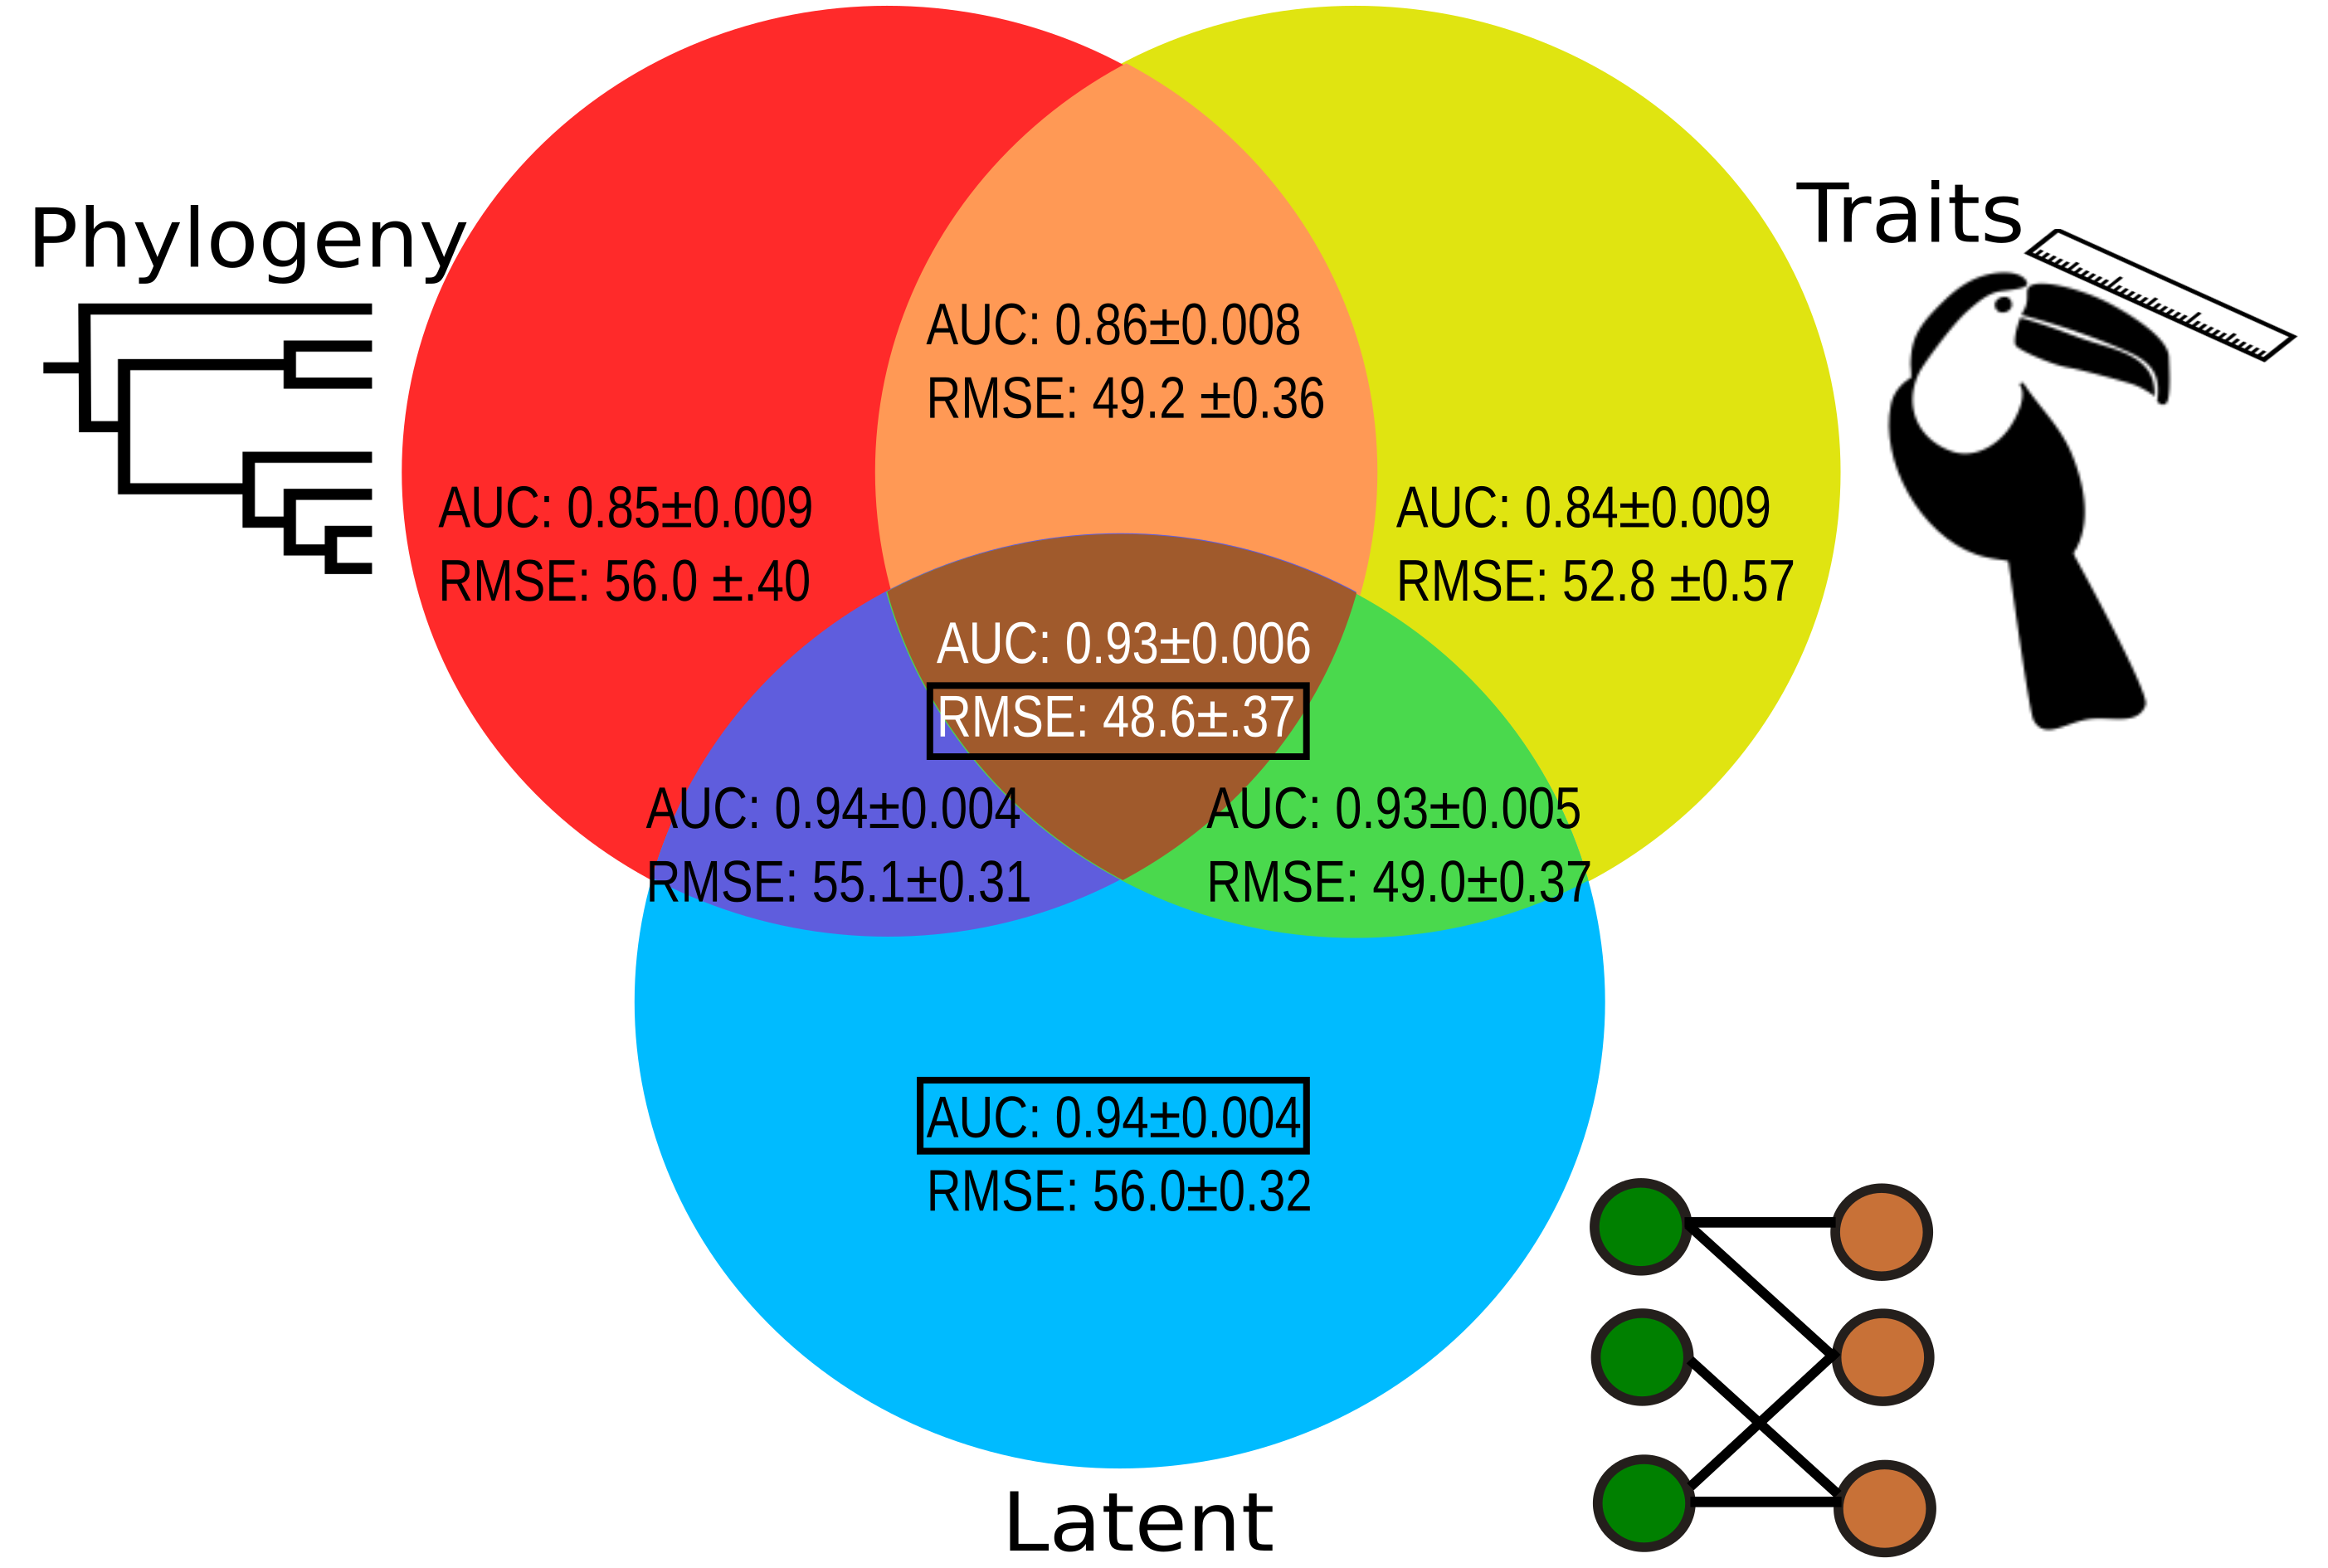
\includegraphics[width=\linewidth]{Fruglink/Figs/ReplicatePerformance_Polytomy.png}
\caption{Summary performance metrics of all 7 models, as measured by area under the receiver operating characteristic curve (AUC) and root mean squared error (RMSE); highest performing models for each metric are outlined in black. Mean metric values are presented from 100 replicates of each model structure alongside standard deviation. Model discriminatory power between links and non-links is maximized by including latent structural features, with the inclusion of trait, phylogenetic information, or both actually slightly decreasing discriminatory power. However, inclusion of trait and phylogenetic information, while not improving AUC, does increase overall model accuracy as measured by mean root squared error.}
\label{fig:Figure_1}
\end{figure}


\clearpage 

\begin{figure}%[tbhp]
\centering
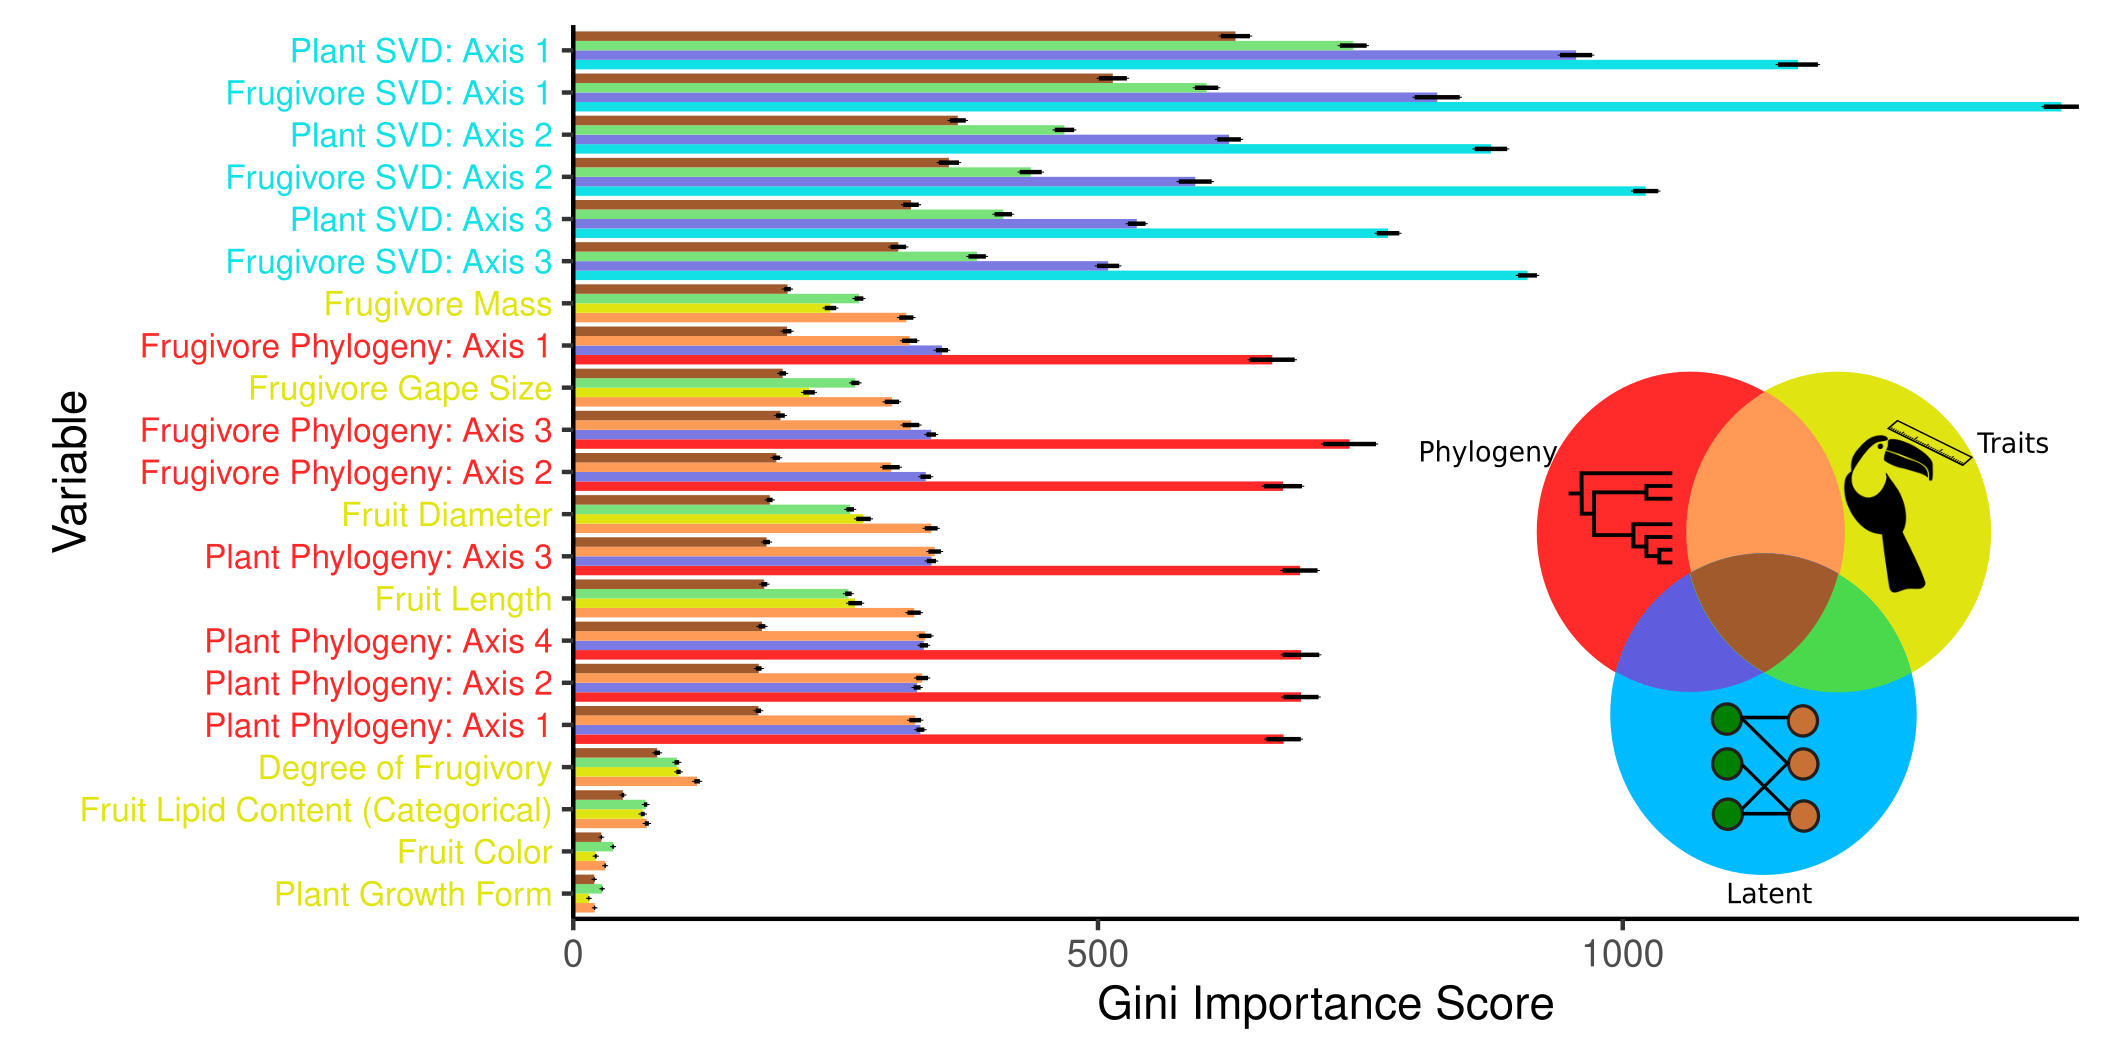
\includegraphics[width=\linewidth]{Fruglink/Figs/VarImportance_ErrBars_Short.png}
\caption{Variable importance across all models as measure by Gini importance score; color scheme is consistent with figure 1. In all models that include them, latent traits were consistently the most important variables for prediction. These were followed by continuous frugivore traits (body mass, gape size), and frugivore phylogenetic axes. Plant phylogenies and continuous trait information were generally less important for prediction than frugivore traits. Categorical plant traits (Lipid content, fruit color, growth form) were the least important variables for prediction.}
\label{fig:Figure_2}
\end{figure}



\clearpage 


\begin{figure}%[tbhp]
\centering
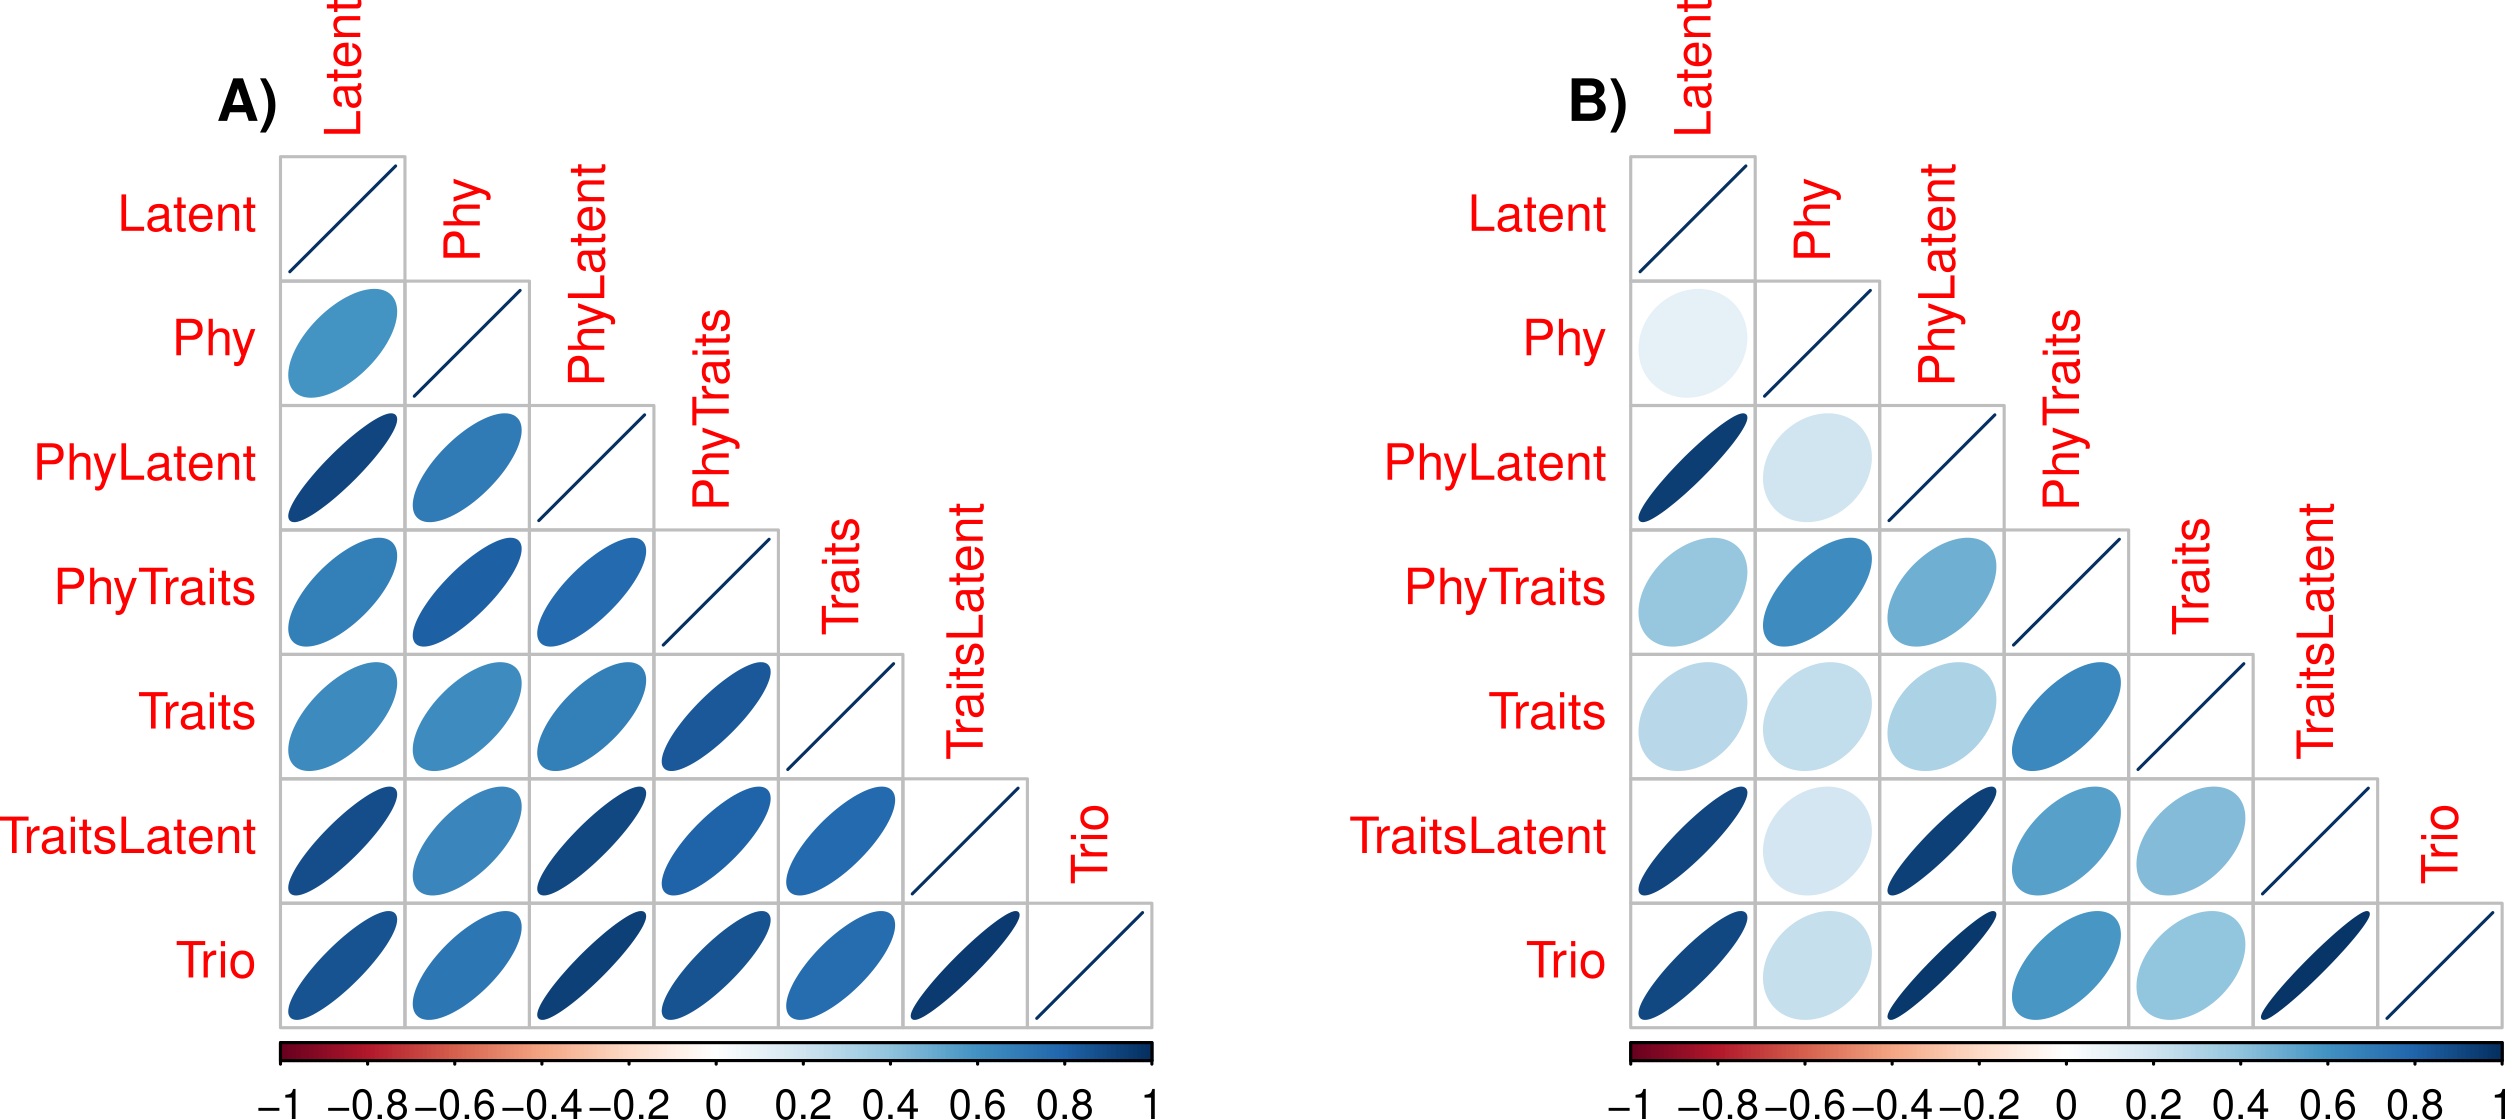
\includegraphics[width=\linewidth]{Fruglink/Figs/SpearmanCorplot_nolab.png}
\caption{Pairwise Spearman's rank correlations of link suitabilities across models for all potential interaction (A), as well as only unobserved interactions (B). The latter set of links represents both true forbidden links, as well as other potential interactions not observed in our data-set.}
\label{fig:Figure_3}
\end{figure}                             
                                                
                     
                          
\addtocontents{toc}{\protect\vskip-20pt}
\chapter[The impacts of geographic range size and niche breadth on species centrality in floral visitation networks]{The impacts of geographic range size and niche breadth on species centrality in floral visitation networks\footnote{In revision at \textit{Proceedings of the Royal Society: B}. Reproduced here under the CC BY 4.0 license terms. See Appendix D.}}   



\section*{\textbf{\underline{Abstract}}}
Understanding the factors that influence species' roles within ecological networks can provide insights into the rules governing the assembly of interaction networks. Centrality, a property describing how connected a given node is to the rest of a network, is often used to identify species whose loss may result in disproportionate effects on biotic communities. Understanding the drivers of species' centrality in floral visitation networks is crucial for understanding network responses to global change. Here, we test how geographic range size and niche breadth influence species centrality in floral visitation networks across spatial scales. We combine a globally distributed dataset of floral visitation networks comprising 30,330 interactions among 6,857 species with large-scale occurrence data to evaluate how species’ geographic and environmental range sizes impact their role in networks across scales. In global metawebs we observe a strong positive effect of geographic range size on closeness centrality, but that effect largely disappeared after accounting for spatial turnover in interactions. Instead, niche breadth showed a positive relationship with the standardized centrality of flowering plant species in both network types. Site-level centrality was tightly linked to species ranges. Together, these results emphasize the need for a multiscale perspective to understand the drivers and consequences of changes in ecological network properties across environments and scales.


\section*{\textbf{\underline{Introduction}}}

\paragraph*{}
Originating in mathematics, graph theory perspectives have become increasingly popular for the study of ecological networks throughout recent years \parencite{bascompte2007plant, landi2018complexity, valdovinos2019mutualistic, guimaraes2020structure}. Under this framework, interacting species can be represented as a series of nodes connected by links (interactions). What constitutes an ``interaction" is variable, set by the context of the system, and may include predation events, infections \parencite{dallas2017predicting}, floral visits \parencite{Young21}, or any number of other biotic interactions. By quantifying the full set of links present in a given system, we have gained insights into the structural properties of species interaction networks that allow us to better predict their potential responses to change \parencite{gilarranz2017effects}. For example, foundational work has linked network properties such as nestedness (the tendency for species with few interactions to link to species with many other interactions) and modularity (the tendency for species to interact more within given groups or ``modules'' than between them) to features such as network stability in response to perturbations or species extinctions \parencite{okuyama2008network, thebault2010stability, suweis2013emergence}.




\paragraph*{}
%TS: Species Centrality in Empirical Networks is important, and people try to predict it
In addition to these network-level properties, we can also measure the contribution of an individual node to overall network structure considering node-level properties. One of the most commonly analyzed node-level properties is centrality: a suite of measures describing how connected a given node is to the rest of the network. Highly central species may represent keystone species in a network, and removal of these nodes is likely to have outsized impacts on their associated communities \parencite{traveset2017plant, maia2019plant, martins2024propagation}. Identifying the eco-evolutionary processes that give rise to highly central species in local and regional-scale interaction networks is essential for understanding how ecological networks are organized and how they may respond to disturbances \parencite{moulatlet2023species, martins2025determinants, zhang2025network}. Previous work has emphasized the importance of species traits \parencite{watts2016influence, lazaro2020linking, maia2019plant} and evolutionary history \parencite{Gonzales2015macroecology, burin2021macroevolutionary} on influencing both network and node-level properties. Investigating determinants of a species' role within floral-visitation networks (defined here as its position and the distribution of interactions relative to other members in a network, captured through node-level properties such as centrality), can provide insights into biological processes underpinning interaction network structure across scales. Understanding these drivers in the context of floral visitation networks, which are often characterized by interaction generalism \parencite{waser1996generalization,stanton2003interacting} and frequent facultative interactions \parencite{geib2012tracing}, is of particular conservation importance as global declines in pollinator abundance and diversity threaten to potentially reduce pollination services in many ecosystems \parencite{potts2010global, rodger2021widespread}. 


%TS: Geographic range size may be associated with species role in a network. 
\paragraph*{}
In addition to morphological characteristics and phylogenetic history, the size of a species' geographic range may also impact its role in pollination networks at both local and global scales \parencite{moulatlet2023species, dattilo2020species}. 
% TAD: what does "its" in the sentence above refer to? I see what you're doing with the transition, but it's pretty awk. 
% GF: Rewrote. Still has an "its", but hopefully more clear. 
As species ranges increase in size, so does the total number of potential interaction partners. As a consequence, in regional metawebs (the set of species interactions observed across multiple local webs \parencite{poisot2012dissimilarity}) wide-ranging species may increase in their total number of interactions as both potential partners and interactions turn over across space \parencite{fricke2020accelerating, martins2022global}. 
% TAD: so now we have 2 different flavors of metaweb, regional and global?
% GF: I'm hoping that I can use "regional" as a catch-all (to have a metaweb you have to choose an "region" [extent] to aggregate over. In our case that's the globe. 
This accumulation of interactions across area, parallel to the classical species-area relationship \parencite{burkle2012shifts,sugiura2012scale, galiana2018spatial, dallas2021species}, may thus induce positive associations between species range size and species centrality at regional or global scales.
% TAD: but people have done interaction scaling, so why just be like "similar to species-area relationships"? You don't even have to cite my shit here if you don't want to, but I've done it. 
% GF: Hm; I was trying to reference the interaction-scaling lit here but maybe made things weird with the species-area relationship comparison. The citations here are mostly 
Additionally, species with broad geographic ranges may also be more central in local networks if geographic range size is associated with demographic or functional traits that may allow for generalist interaction strategies or high local abundance \parencite{holt1997relationship, hurtado2024generalism, Moulatlet2025General}. This potential confounder makes it difficult to differentiate the potential reasons geographic range size may impact species roles in mutualistic networks. The development of null modeling approaches, in which many random permutations of network linkages are summarized into an observed distribution of potential network property values, has been instrumental in making meaningful comparisons across ecological networks of different size and connectance \parencite{dormann2017, guimaraes2020structure, bluthgen2024critical}. Here, we utilize a null modeling approach in order to tease apart the otherwise confounding effects of turnover and range size \textit{per se} on species centrality across scales. 



\paragraph*{}
% We can think of "range size" geographically or environmentally
Species' geographic range size is driven by a number of biogeographic factors, including evolutionary history \parencite{webb2000geographic, alzate2025evolutionary}, dispersal limitation \parencite{alzate2022understanding}, biotic interactions \parencite{pigot2013species,galiana2023climate}, and climatic constraints \parencite{hausharter2023niche}. As species increase in the geographic extent they occupy, they may geographically overlap with more potential partners, increasing their centrality. However, geographic range size might not be the strongest predictor of the number of potential partners. Instead, species that occur in more climatically diverse environments may co-occur with a larger set of potential partners \parencite{slatyer2013niche, batstone2018using}. Therefore, species with broad abiotic niche breadths may have higher centrality in the global metaweb as a function of greater niche overlap with potential partners. A positive relationship between niche breadth and local centrality may also be observed if climatic and interaction generalism are positively associated, a feature observed in some food web systems \parencite{slatyer2013niche}. Niche breadth and geographic range size are fundamentally linked, though the exact shape of the relationship is dependent on the geographic availability of environments across space \parencite{dallas2025linking}.



%TS: Centrality means different things at the local and regional scale
\paragraph*{}
Biologically, species centrality has a fundamentally different meaning in local networks and global metawebs, and understanding how centrality scales between these contexts is still an open question in network ecology. Most existing work investigating the determinants of species centrality within networks to date has focused on local scales (\parencite{maia2019plant}, but see \parencite{moulatlet2023species}), as here node centrality has clear links to network properties \parencite{gonzalez2010centrality, maia2019plant, cagua2019keystoneness}. Species that occur in many local networks and are highly central in many or all of them may also exhibit high centrality in regional or global metawebs ( \parencite{estrada2007characterization, martins2025determinants} though see \parencite{dallas2022parasite}). However, even species with low local centrality can achieve high centrality in the global metaweb if they exhibit high interaction turnover across a wide geographic area \parencite{carstensen2014beta, simanonok2014partitioning}. At a global level, these central species may appear as relative generalists with many potential partners. However, at local scales, the realized set of interactions of any given individual or population may be relatively narrow \parencite{bison2015upscaling, arroyo2023intraspecific}. As such, understanding how centrality scales from local to global scales helps us better understand how population-level interaction patterns may vary across mutualistic species' ranges. 




% thesis
\paragraph*{}
To address these questions, we quantified variation in species-level centrality relative to geographic and environmental range size across a global assemblage of avian-plant and insect-plant floral visitation networks. Specifically, we tested whether species with broader geographic ranges or environmental niches occupy more central positions within local networks or global metawebs. We predicted that centrality will increase with range size and niche breadth in both contexts (Figure \ref{fig:conceptCentralRange}). At the metaweb scale, we expected species with broad ranges to turnover in interactions across geographic or environmental space, allowing them to accumulate more interactions across sites. At the local scale, we predicted a similar positive relationship driven by the positive association between interaction generalism and climatic or habitat generalism. Finally, we investigated whether these relationships persist after using null-model approaches to account for the impact of species co-occurrence on potential centrality measures. If range size or niche breadth continues to be positively associated with centrality under null models that control for co-occurrence, it would suggest a fundamental link between geographic or climate distributions and factors determining species role within mutualistic networks. Together, our results suggest that the impacts of range size on species centrality in large-scale metawebs are primarily driven by interaction turnover and the scaling of interaction specificity from local to global networks. When variation in interaction turnover is incorporated, niche breadth exerts the strongest positive effect on plant centrality within global networks. Consequently, species with large geographic ranges may appear to be relatively generalist in global metawebs due to high interaction turnover, but local-scale interaction patterns may exhibit more nuanced and variable relationships with species range limits. 

%----------
\section*{\textbf{\underline{Methods}}}

\paragraph*{Data}\mbox{}\\ 
We queried floral visitation networks through the Web of Life dataset, resulting in 97 networks with a total of 30,330 unique interactions between 6,857 species. We combined these networks into two global metawebs: one describing avian-plant interactions and another describing insect-plant interactions. Most studies only characterized one of these types of interactions; for the three studies that reported both insect and avian floral visits, we divided the network as appropriate. The avian-plant metaweb is comprised of 2,033 unique species-level interactions between 605 plant and 120 bird species across 31 sites. The insect-plant metaweb is larger, consisting of 28,297 interactions between 1,960 plants and 4,182 insect species across 66 sites. While expert range maps are available for most birds and some well-studied plant taxa, the majority of species in our study do not have up-to-date expert species range estimates available. In order to investigate the role of range size in determining species-level network traits, we estimated species ranges from available occurrence points. 

\paragraph*{Estimating Geographic Range Size}\mbox{}\\ 
For each species, we queried global occurrence records from the Global Biotic Information Facility (GBIF) using the \textit{gbifdb} $R$ package. Occurrence points were first processed using the \textit{coordinateCleaner} package; points were removed if they were present only in the fossil record, occurred within 2 km of country centroids, were not terrestrial, or were marked as an ``introduced" individual. To avoid overestimating species range size through including spurious or transient records in GBIF, we used a quantiled minimum convex polygon (MCP) approach. Within each continent -- based on a 7 continent model (Asia, Europe, Africa, Oceania, North America, Antarctica, and South America) -- we created the smallest minimum convex polygon that contains the central 95\% of the occurrence points within each continent. Range polygons were not created for species-continent combinations with less than 10 occurrence points. Total species' geographic range size was calculated as the total terrestrial area occupied across all continents. The points included within these polygons were also used for the calculation of environmental range (below). 2,554 species within our network had insufficient occurrence data to create species ranges; leaving a total of 4,303 species within our analysis (110 birds, 2,126 insects, and 2,067 plants). 


\paragraph*{Estimating Niche Breadth}\mbox{}\\ 
For each occurrence point, we extracted 56 climatic values from WorldClim at a 2.5 arc-minute resolution \parencite{fick2017worldclim}. These values represent a number of climatic variables potentially important for limiting species' distributions, averaged across the years 1970-2000. As these variables represent a high-dimensional environmental space that is collinear in many aspects, we performed a principal component analysis in order to reduce the dimensionality of our niche space \parencite{kriticos2014extending, dallas2025linking}. The first two principal components of this climatic space explain over 77\% of the total climatic variation. For each species, we plotted each occurrence point that fell within the 95\% quantiled geographic range polygon calculated above onto the Cartesian plane defined by these two PCA axes, combining points from all continents on which a species occurred. We then again employed a minimum convex polygon approach to draw an environmental range in this PCA space for each species (i.e., its niche breadth).

\paragraph*{Centrality Measures}\mbox{}\\ 
Insect and avian floral visitor metawebs contained 6142 and 725 total species, respectively. The vast majority of species in each network were connected to one major component (the largest set of interconnected nodes). As centrality measures become non-comparable in unconnected graphs, we dropped species that were not part of these major components. This resulted in the removal of 51 (0.83\%) and 4 (0.55\%) species from the insect and avian metawebs, respectively. Closeness centrality (which describes the mean proximity of one node to all other reachable nodes within the network, Figure \ref{fig:conceptCentralRange}) was calculated for nodes in the remaining simply connected networks using the \textit{igraph} package. 
% TAD: why give a weirdly technical def of closeness? It's not wrong or bad, but you want plant-frugivore folks reading this. It's proportional to the mean proximity of one node to all other reachable nodes in the network. GF: Casual-ified! 
We chose closeness centrality as an intermediate between hyper-local measures of centrality (e.g., degree centrality) and hyper-global measures (e.g., eigenvalue centrality). At the global metaweb scale, the rank of alternative measures of centrality were positively correlated, though to varying degrees (Figure \ref{fig:S2}).

\paragraph*{Null model expectations of species centrality}\mbox{}\\ 
While centrality measures are designed to be comparable between nodes of the same network, their absolute value is heavily influenced by network size and connectance, potentially hindering comparisons across networks. To address this when measuring species-level centrality in local networks, we used a null-model approach to standardize centrality within each local network. For each local network, we first measured the closeness centrality of all component species species using a similar approach to the global metaweb.
% TAD: you use lots of possessives (e.g., 'its') and it makes it read weird. If that's just your style, stick to it, but I am not a fan. 
%GF: Took out a couple of the most confusing ones; hopefully the remaining ones are relatively clear. 
We then used the \texttt{vegan} package to generate 1000 randomized versions of each local network by permuting interaction links while preserving each node's degree (effectively preserving marginal totals of the interaction matrix). This allowed us to characterize the potential distribution of centrality values for each node, given that node's degree and the network's overall structure. We then $z$-transformed the observed centrality values using the mean and standard deviation of this null distribution to create a $z-$transformed measure of local closeness centrality for each species-site combination. 


\paragraph{} To extend this approach to the metaweb level, we pooled permuted local webs to construct null global metawebs. This allowed us to generate a null distribution of species-level closeness centrality across the entire metaweb, accounting for each species' presence across multiple local networks. Observed metaweb centrality values were then $z-$transformed relative to this distribution. We investigated both measured and $z-$transformed centrality at the metaweb scale. At the local scale we only modeled $z-$transformed centrality, as raw measures of centrality are not directly comparable across differently sized networks. One insect-plant and three avian-plant networks were too small to create realistic null distributions, and were subsequently excluded for local centrality analyses. 


\paragraph*{Statistical Analyses}\mbox{}\\ 
We examined the role of species range size and niche breadth on species centrality through Bayesian generalized linear models implemented in Stan \parencite{carpenter2017stan} through the $R$ package \textit{brms} \parencite{burkner2017brms}. In order to facilitate comparison and meaningful interpretation of interaction effects, both geographic range sizes and niche breadth values were log-transformed and then rescaled to a mean of 0 and standard deviation of 1. All models therefore shared the generalized form of predicting a given species' centrality as a function of geographic range size, niche breadth, and the interaction between these predictors. Niche breadth or geographic range size may exert fundamentally different effects on the centrality of flowering plant species compared to floral visitors. As such, we analyze node types (floral visitor or flowering plant) separately for each network or set of networks, effectively repeating our modeling approach for all factorial combinations of: scale (metaweb vs local webs), network type (insect-plant vs avian-plant), and interactor type (floral visitor vs flowering plant). Accounting for our two alternative centrality measures at the metaweb scale (measured and $z-$transformed closeness centrality), this resulted in 12 models total. We use vague priors centered on 0 for all slope and intercept coefficients. All models were fit using 5 Markov chain Monte-Carlo simulations, each with 5,000 iterations following a 1,000 iteration burn-in period; posterior samples were sampled without thinning \parencite{link2012thinning}. Simulation convergence was checked through visual inspection of traceplots. Gelman-Rubin statistics fell below 1.01 for all parameters across all models.  For slope terms we sampled the resultant posterior distributions and approximated the two-sided posterior probability ($POP_2$) as twice the proportion of posterior samples falling above or below 0 (whichever is smallest), a Bayesian analog to traditional frequentist p-values \parencite{shi2021reconnecting}. Relationships between fit slope values across models are presented as pairs plots in supplemental figures \ref{fig:S6}-\ref{fig:S11}. 

\paragraph{}
For the subset of species which occurred across multiple sites, we further investigated the role interaction turnover may play in determining species centrality in global metawebs. As both the degree of turnover and number of sites at which a species occurs may have nonlinear effects on metaweb centrality, we investigate these factors through a generalized additive modeling (GAM) approach. For each node the that occurred in multiple sites (1,166 species), we calculated the Simpson's dissimilarity of interaction partner sets across all sites in which they occurred \parencite{baselga2015comparing}, as implemented in the $R$ package \texttt{betapart} \parencite{baselga2012betapart}. We created GAM models predicting metaweb centrality (either raw values or $z-$transformed, scaled to a mean of 0 and standard deviation of 1 to facilitate comparisons across models) as a function of the tensor product of interaction turnover and number of local sites. We investigate the $p-$value of tensor terms, as well as compare estimated degrees of freedom to maximum allowable degrees of freedom ($k'$) as well as visually inspected model residuals to assess model fit. %Plots illustrating the resultant partial effects of turnover across are show in Figure \ref{fig:gam}. 

% TAD: have you defined k'? might be worth just spelling it out instead of the notation. You want the reader to follow, and you've already been talking about tensor products. 
% GF: Definition added


% -------------------
\section*{\textbf{\underline{Results}}}

\paragraph*{Species Occurrences and Interactions}\mbox{}\\ 
Species' geographic range sizes in insect-plant networks varied widely, ranging from 2,232 km$^2$ (\textit{Chaetanthera lycopodioides}, a range-restricted montane Aster endemic to Chile and Argentina \cite{arroyo2007display}) to over 119 million km$^2$ (\textit{Sonchus oleraceus}, a cosmopolitan weed native to Eurasia), with a median value of 3,749,391 km$^2$. Geographic distributions of species in avian-plant visitation networks ranged from 2,518 km$^2$ (\textit{Barbacenia longiflora}, a monocot forb restricted to Minas Gerais, Brazil) to over 85 million km$^2$ (\textit{Prunella vulgaris}, a cosmopolitan invasive weed), with a median value of 1,536,647 km$^2$. Across sites, geographic and environmental range size were positively correlated ($r$=0.667, $p <$ 0.001). Typical of large-scale interaction metawebs, realized connectance (the percentage of realized links out of the total possible number of interactions) was low \parencite{jordano1987patterns}. At the global scale, only 0.32\% and 2.8\% of potential links were realized in insect and avian interaction metawebs, respectively. At the site-level, average connectance of insect-plant networks was 0.194, whereas average avian-plant network was 0.356. 

% TAD: numbers don't go in math font unless you're willing to put every number in math font. 
%GF: Fixed

%TD: what the fuck is POP_2? 
%GF: I put the explanation of this at the very end of the methods, but it is a weird metric. It just seemed like a better for shorthand for "our 95% Credible Interval does or doesn't overlap 0" as well as being a closer analog to like hypothesis testing. But keeping it isn't a make or break for me. 
% TD: eh. Give it a cooler name? \omega_{95}? Idk man. 


%Effect in metaweb
\paragraph*{Global Metawebs}\mbox{}\\ 
At the metaweb scale, geographic range size was positively associated with species centrality of all node types across both insect and avian networks (Figure \ref{fig:MetawebEffect}). However, once accounting for potential co-occurrence through $z$-transformation, geographic range size showed no association with metaweb centrality for avian or insect floral visitors, or insect-visited plant species, and instead showed a negative association with the centrality of avian-visited plant species ($POP_2=$0.020). Niche breadth had a negative impact on centrality for plants and insects within the insect-plant metaweb after controlling for geographic range size ($POP_2<$0.001, $POP_2=$0.028). After $z$-transformation, niche breadth instead had a positive impact only on plant centrality in both insect and avian metawebs ($POP_2<$0.001 across both networks) while showing no effect for floral visitors. There was no significant interaction effect between geographic range size and niche breadth on unstandardized metaweb centrality across node types. However, after $z$-transformation, plants in both network types showed positive interaction effects ($POP_2<$0.001 and $POP_2=0.009$ for insect and bird-visited plants, respectively).



\paragraph{} For species that occurred across multiple sites, interaction turnover varied from 0 (complete conservation or nestedness of interactions across sites) to 1 (no overlap in interactions across sites), with a mean value of 0.644. The tensor product of interaction turnover and number of sites was statistically significant in predicting both raw and $z-$transformed metaweb centrality ($p<0.001$), but varied widely in the amount of variance explained. For the GAM model predicting measured metaweb centrality $R^2=0.231$, with interaction turnover exhibiting a positive partial effect across much of the realized parameter space, particularly for species with the highest centrality values (Figure \ref{fig:gam}). After $z$-transformation, the tensor product of turnover and number of sites still exhibited a statistically significant effect ($p<0.001$) but explained little of the overall variation ($R^2=0.054$). Taken together these results further suggest that positive relationships between species' geographic range size and measured metaweb centrality are largely driven by interaction turnover across sites. 



%Effect on local webs
\paragraph*{Local Webs}\mbox{}\\ 
Average species centrality in local floral visitation networks was positively correlated with their centrality in their respective global metawebs ($r=0.480$ and $p<0.001$ for insect webs, while $r=0.079$ and $p=0.035$ for avian webs). Species that occurred at multiple sites showed variable centrality across their respective local webs (Figure \ref{fig:S3}). Geographic range size was negatively related to the local centrality of insect-visited plant species (Figure \ref{fig:LocalPlot}, $POP_2=$0.018). Conversely, niche breadth was positively related to the average local centrality of nodes within insect networks ($POP_2<$0.001 for plants, $POP_2=$0.004 for insects). Insect-visited plants also exhibited a positive interaction term between geographic range size and niche breadth on average local centrality ($POP_2=$0.022). We failed to find any significant effect of range size, niche breadth, or their interaction on the local centrality of species within avian networks.






\section*{\textbf{\underline{Discussion}}}
%The effect of geographic range size on metaweb centrality is mediated through cooccurrence. 
\paragraph*{} Generally we find species' geographic range size and niche breadth are more clearly linked to their centrality in aggregate plant-pollinator metawebs than within local interaction networks. The positive impact of geographic range size on metaweb centrality we observed across all node classes may be caused by a number of potential drivers. Species with broad geographic ranges are likely to co-occur with more potential interaction partners across their range (Figure \ref{fig:S4}). In this case, even if species are relatively peripheral across local networks, they may be relatively central at the metaweb level if interaction turnover is high across their range \parencite{martins2025determinants}. Our results support this interpretation, as while species with large geographic ranges tended to be more central in the global metaweb, they did not tend to be more central than null expectations based on their connections across all local webs (Figure \ref{fig:MetawebEffect}). Additionally, generalized additive models indicated a large partial effect of interaction turnover on measured metaweb centrality, but this affect largely disappeared once these centrality values were $z-$transformed (Figure \ref{fig:gam}). Together, these patterns suggest that, at the global scale, species centrality in these metawebs is shaped more by neutral processes-namely the accumulation of interactions across space-than by the specific identity of those interactions. 

\paragraph*{}
Contrary to our expectations, standardized centrality was negatively related to geographic range size of plants in avian-plant networks after accounting for niche breadth. This pattern may indicate slower accumulation of interactions across space (lower interaction turnover) than otherwise expected. This pattern may be driven by wide-ranging, disturbance-adapted species that occur in many networks but are less likely to form interactions with narrowly distributed specialists. Nectarivory has evolved numerous times within birds, but contemporary biogeographical distributions of avian nectarivore diversity is clustered in the neotropics and parts of Australasia \parencite{kissling2012bird}. This spatial clustering of potential partner diversity may drive lower rates of interaction turnover of avian-pollinated plants across large spatial scales. 

%The effect of environmental range size only impacts plants (mostly when $z-$transformed). 
\paragraph*{}
After $z$-transformation, metaweb centrality was positively related to niche breadth in plants of both metawebs, but was unrelated in floral visitors. If plant species are limited in their dispersal by the availability of mutualists \parencite{warren2014mutualism, duffy2017specialized}, species with broad ranges of potential partners may be able to exploit a more climatically diverse set of environments. The availability or efficacy of mutualists may increase the abiotic tolerances of some species \parencite{warren2014mutualism, fowler2023geographic}, effectively expanding their climatic niche breadth. Batstone et al. (2018) outline how environmental variability may favor interaction generalism by altering the availability or efficacy of mutualists \parencite{batstone2018using}. Similar mechanisms may occur across an organism's range; plants with climatically diverse ranges may experience parallel changes in partner availability or efficacy, promoting interaction generalism \parencite{hurtado2024generalism}. Alternatively, in systems characterized by widespread generalism, plant species with broad niche breadths may participate in more interactions as they co-occur with a broader complement of potential pollinators. Understanding the mechanisms of this interplay between a species' climatic niche breadth and its position within local and global networks warrants further study. 

\paragraph*{}
In contrast to global metawebs, both geographic range and niche breadth show a reduced effect on species centrality at the local scale. In insect networks, average local centrality was positively related to niche breadth across both node types, but negatively related to geographic range size in insect-visited plant species. We also detected a positive interaction between range size and niche breadth on the centrality of plant species in insect-floral visitation networks, indicating that their combined influence shapes local structure of these networks (Figure \ref{fig:LocalPlot}). Species with broad geographic ranges tended to be more central when they also had broader climatic niches, whereas species with narrow ranges were more central when they exhibited broader niche breadths. This suggests multiple ecological pathways or strategies that may result in high centrality in local networks. Widely distributed species with broad abiotic tolerances may be relatively generalized in their interaction patterns at local scales, increasing centrality \parencite{hurtado2024generalism}. Alternatively, narrowly distributed climatic specialists may also be highly central, potentially through achieving high abundance in restricted environments \parencite{suarez2023dispersal}. The functional consequences of a species' centrality within a network may vary greatly across local, regional, and global scales, and further investigation of how centrality scales across levels of organization is of great interest. In our study, networks are either analyzed at the site level, or aggregated into global metawebs. Fully understanding the processes of scaling from local to global requires hierarchical sampling designs replicated across large geographic extents. While understanding the scaling of network properties across space, environments, and time has received a great amount of conceptual attention in recent years \parencite{tylianakis2008global,morales2008effect, burkle2011future,  moulatlet2023species}, the logistical challenges of research across these scales has limited our ability to fully explore these questions in some cases. 

\paragraph*{}
The emergent consequences of a species' centrality may ultimately differ across local to global scales. For example, at local scales the perturbation of highly central species may propagate farther or more strongly through a mutualistic community than the same perturbation applied to more peripheral species \parencite{Cauga2019, delmas2019, martins2024propagation}. Across larger scales, highly central species may play key roles in allowing mutualistic metacommunities to persist \parencite{filotas2010effect}, especially in the face of habitat heterogeneity or disturbance \parencite{prakash2004habitat}. Patterns of interaction turnover across space are closely linked to both the causes and consequences of centrality scaling relationships. While the temporal turnover of mutualistic interactions is fairly well appreciated in phenological contexts \parencite{olesen2008temporal, chavez2020drivers}, empirical patterns of interaction turnover across space, habitats, and environments warrant further study \parencite{tylianakis2017}. 


\paragraph*{}
Understanding the factors that determine species positions in mutualistic networks across scales is a fundamental question in network ecology. Our study identifies geographic range size as a key determinant of species centrality in floral visitation metawebs, largely driven by the spatial accumulation of interactions across sites. At the local scale, we also find that climatic niche breadth interacts with geographic range size to predict plant centrality in insect-plant networks, highlighting the multiple pathways through species may become highly central at the site level. Together, these results emphasize the need for a multiscale perspective to understand the drivers and consequences of changes in ecological network properties across environments. 
\\

\noindent \textbf{Data accessibility}: Data and $R$ code necessary to recreate this analysis is available on on figshare at \url{https://figshare.com/s/ab0b46493fd69cf4a2c8}\\

\section*{\textbf{\underline{Figures}}}

\begin{figure}[H]
    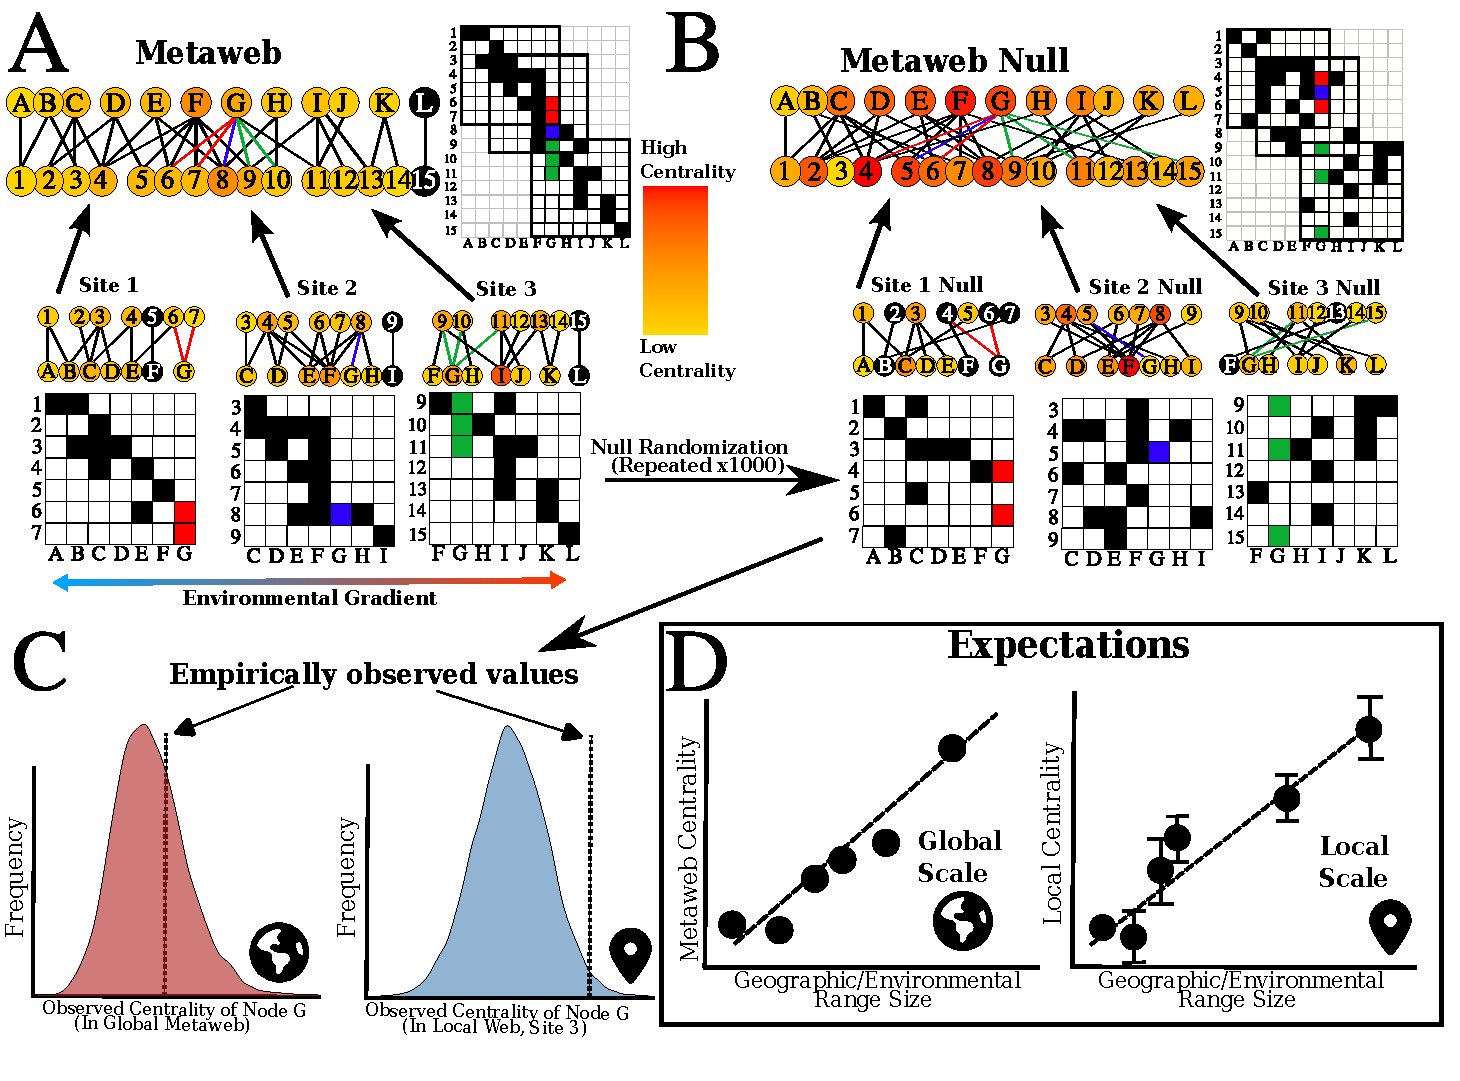
\includegraphics[width=22cm, angle=90, alt={Theoretical diagram summarizing the effects of geographic range size and niche breadth and network centrality across geographic scales}]{centralRange/figs/pdf/Concept_v2_busy_sized.pdf}
    \label{fig:conceptCentralRange}
\end{figure}

\addtocounter{figure}{0}
\begin{figure} [H]
  \caption[Geographic range size and node centrality]{Local interaction networks are embedded along natural environmental gradients (A), with species occurring in one or more sites and contributing interactions to a global metaweb, defined as the union of all observed interactions across sites. At the metaweb scale, species with broad geographic ranges or wide abiotic tolerances may accumulate interactions across multiple sites. At the local scale, such species may also be more central if interaction generalism covaries with environmental or habitat generalism. Species centrality can be quantified within individual site-level networks as well as in the global metaweb (node color). However, metaweb centrality is jointly influenced by the identity of interactions and by interaction turnover across sites. To isolate these effects, we implement a site-level null randomization (B) that shuffles interaction identities within each site while preserving the total number of interactions per species. Repeating this procedure generates null distributions of expected centrality values for each species at both local and metaweb scales (C), given the constraints of observed local network structure. Empirical centrality values can then be standardized (e.g., $z-$transformed) relative to these expectations, allowing scale-dependent effects of range size on network centrality to be evaluated (D).}
\end{figure}

\clearpage 




\begin{figure}[H]
\centering
    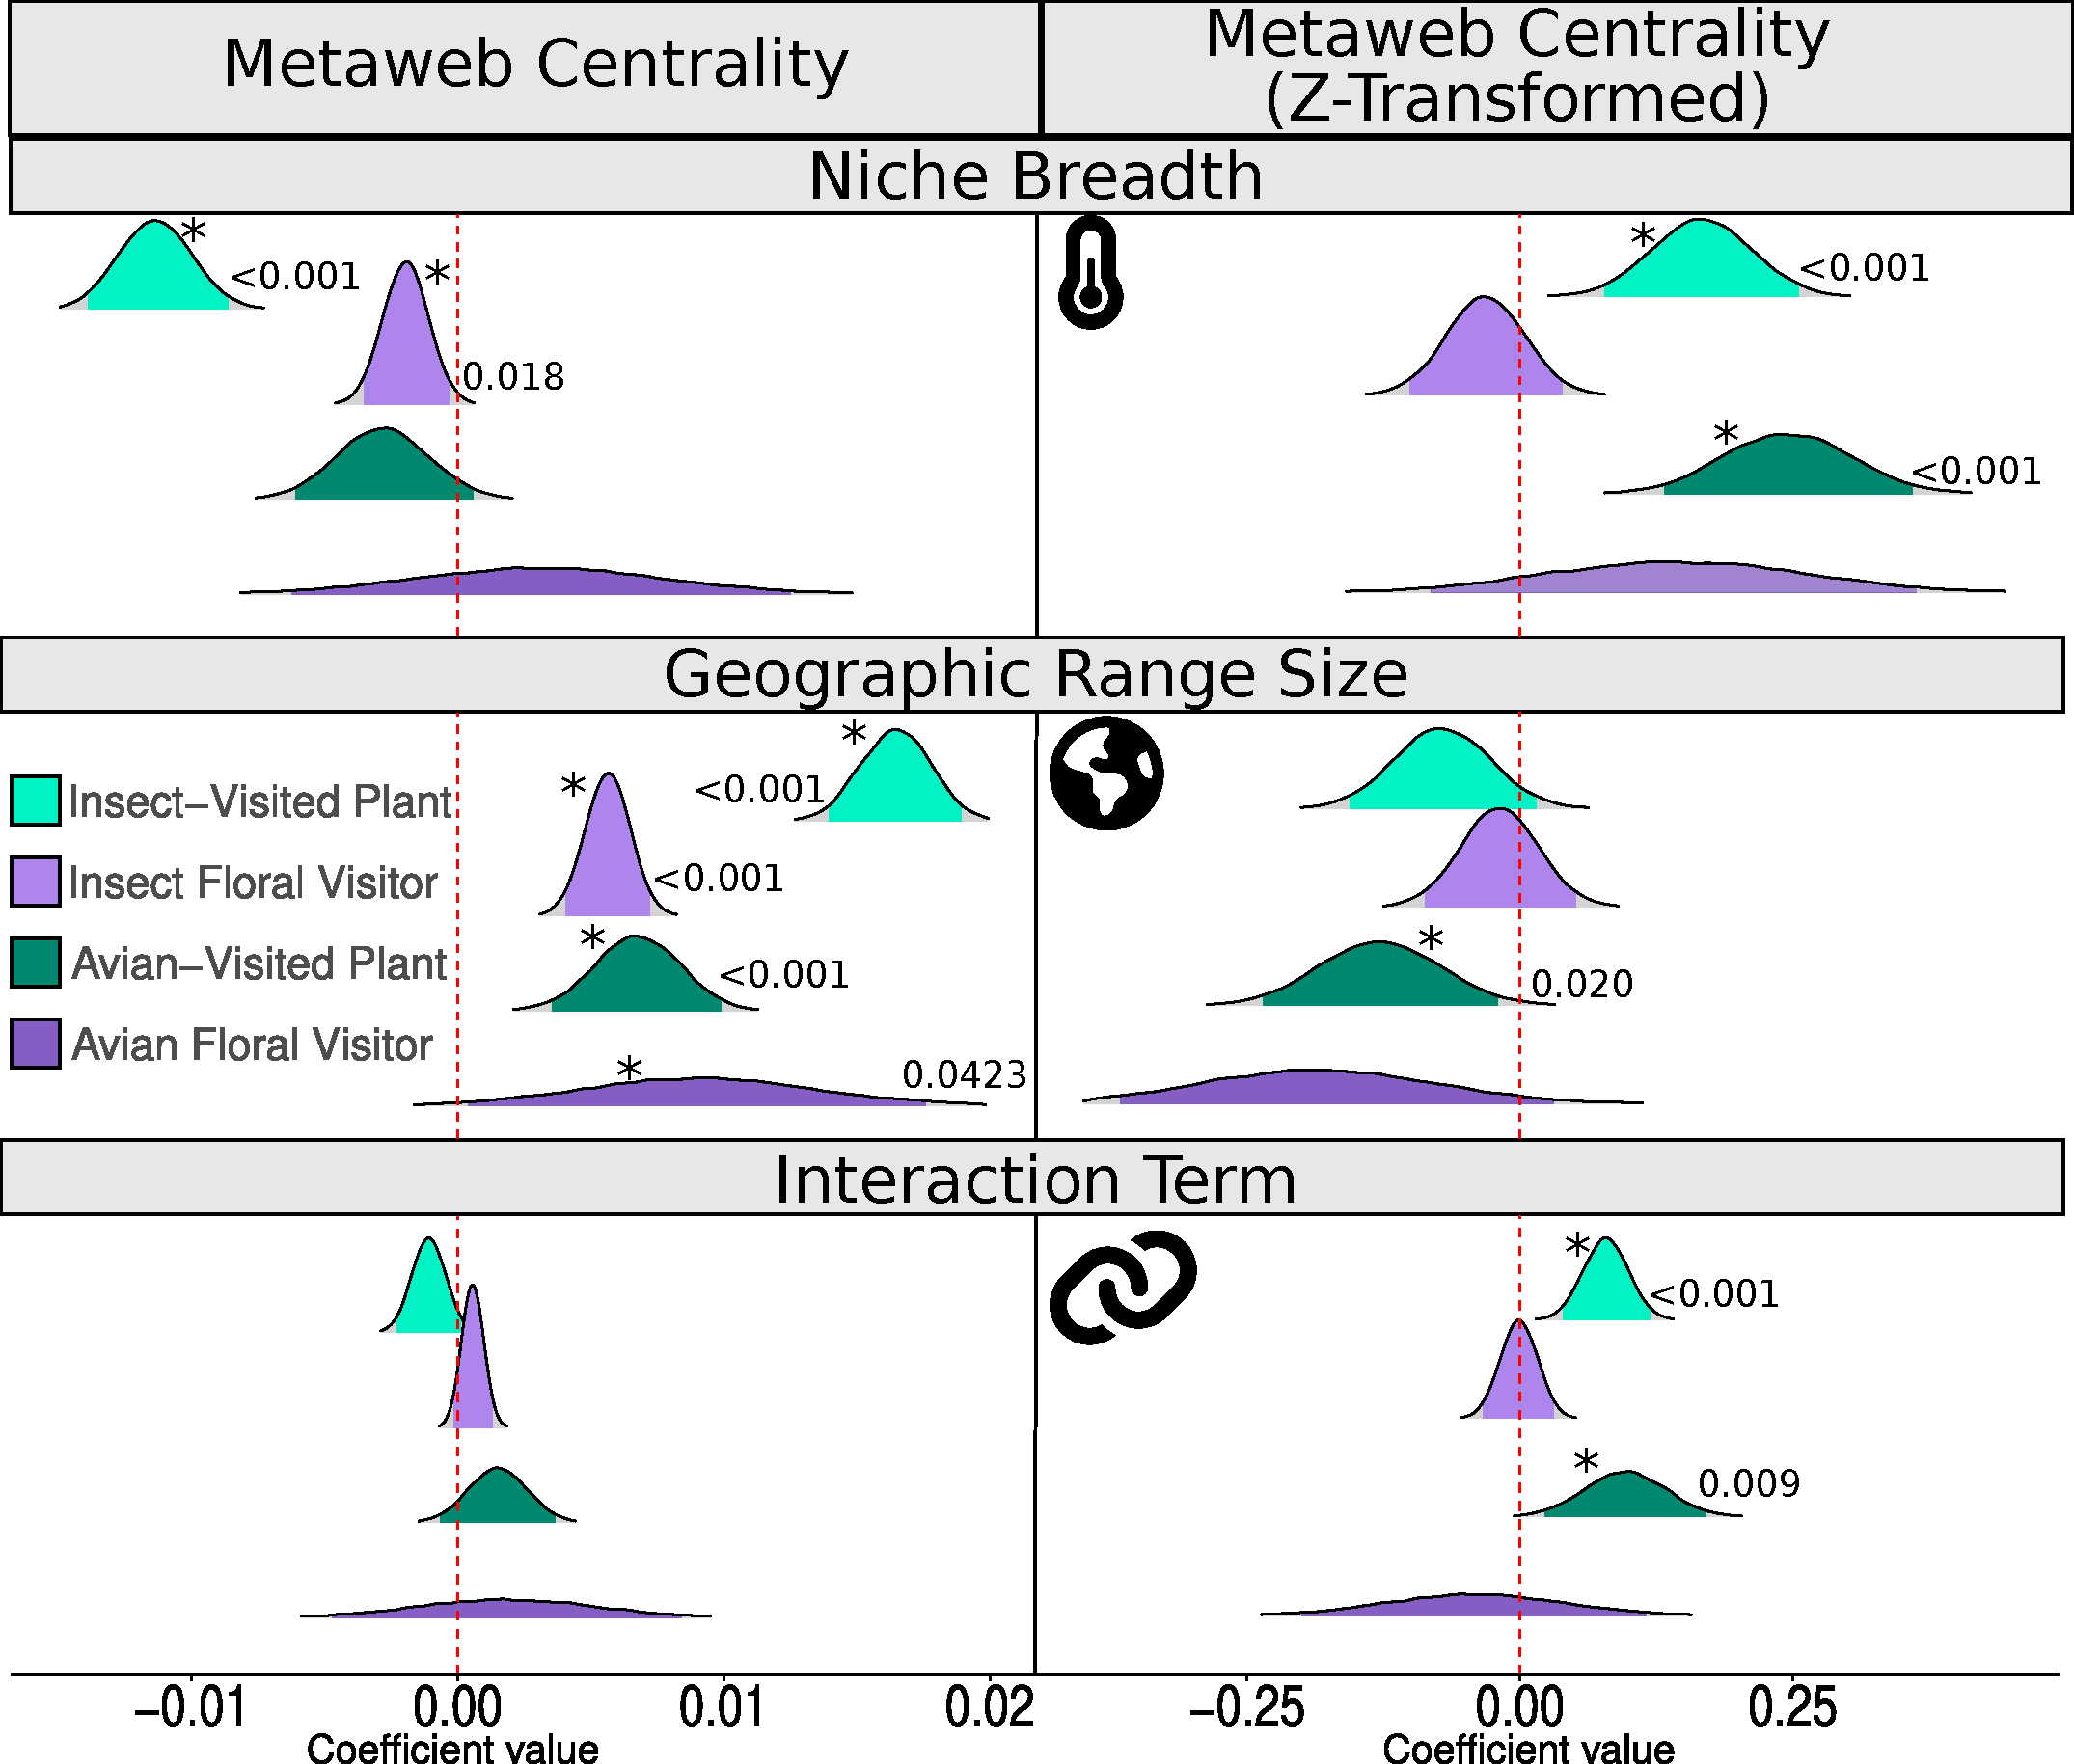
\includegraphics[width=\columnwidth, alt={Sampled posterior slope density curves for multivariate Bayesian generalized linear models of species centrality in the global metaweb}]{centralRange/figs/pdf/Effectplot_Metaweb_Updates.pdf}
    \caption[Sampled posterior slope densities for multivariate Bayesian generalized linear models of species centrality in the global metaweb]{Sampled posterior slope densities for multivariate Bayesian generalized linear models of species centrality in the global metaweb. Colored areas represent 95\% credible intervals of slope terms of the effect of niche breadth (top row, thermometer icon), geographic range size (center row, globe icon), and their interaction term (bottom row, chain icon).  Numbers and asterisks indicate approximate two-sided posterior probability $<0.05.$ Left columns represent models of measured closeness centrality as the response variable; right column represents models predicting centrality values $z-$transformed based on null randomization. After accounting for niche breadth, geographic range size has a strong positive effect of species centrality, but this effect disappears when z-standardized. In plant species, both niche breadth and the interaction between niche breadth and geographic range size positively impact $z$-transformed metaweb centrality.
    }
    \label{fig:MetawebEffect}
\end{figure}

\clearpage 

\begin{figure}[H]
\centering
    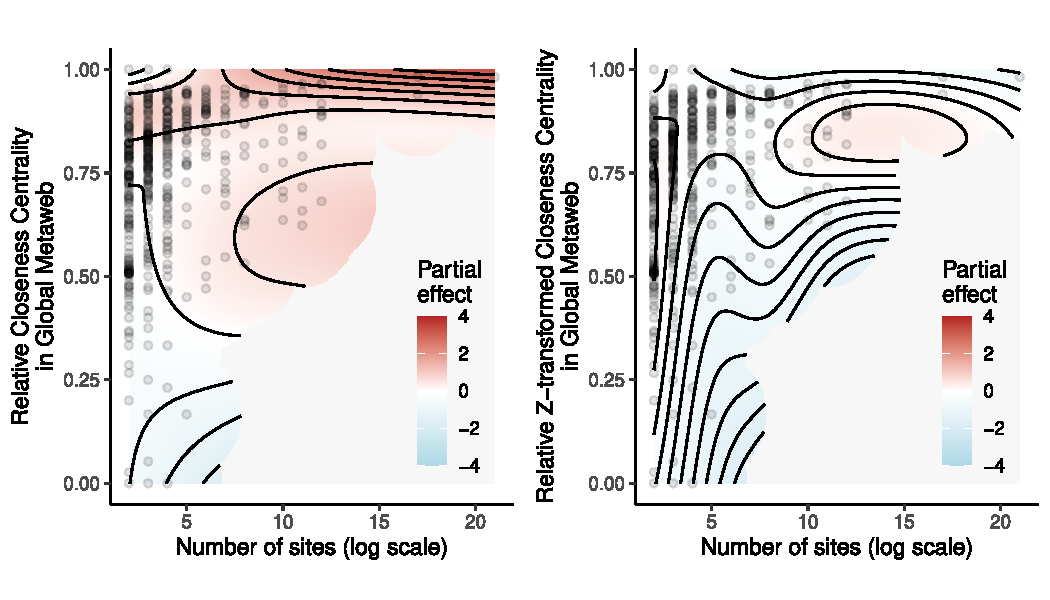
\includegraphics[width=\columnwidth, alt={Contour plot describing effects of interaction turnover on metaweb centrality}]{centralRange/figs/pdf/gamplot.pdf}%
    \caption[Partial effects of interaction turnover on metaweb centrality]{Partial effects of interaction turnover on measured metaweb centrality (left) or $z-$transformed metaweb centrality (right) response values and number of unique local sites, according to fit tensor product GAMs. For comparison, both responses are rescaled to mean of 0 and standard deviation of one. Across the observed range of centrality values, the tensor product of interaction turnover and number of local sites occupied by a species had a positive effect of global metaweb centrality ($p<0.001, R^2=0.231$), especially for the most highly central species. In contrast, after $z-$transformation while the tensor product of turnover and number of local sites a statistically significant negative effect, this relationship explained less than 6\% of variation in metaweb centrality ($p<0.001, R^2=0.054$).}
    \label{fig:gam}
\end{figure}
\clearpage 

\begin{figure}[H]
\centering
    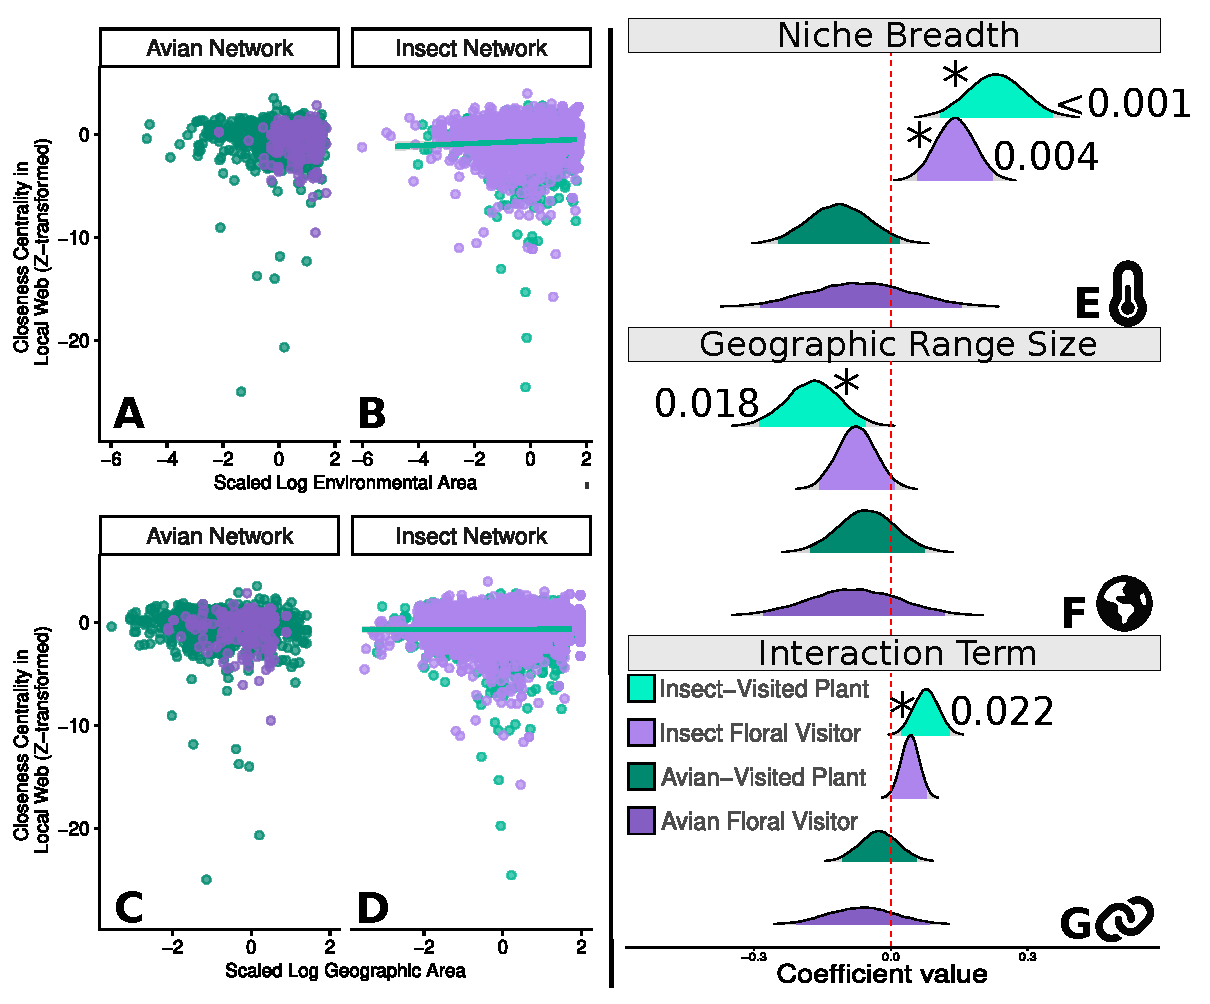
\includegraphics[width=6in, alt={Split figure, where the lefthand side is comprised of scatterplots describing the relationship between centrality in local networks and environmental or geographic range size. The righthand side gives posterior density curves of bayesian generalized linear models of these effects}]{centralRange/figs/pdf/LocalPlot_Composite_v2.pdf}%
    \caption[Relationships between average z-standardized centrality in local networks, geographic range size, and niche breadth]{Relationships between average z-standardized centrality in local networks, geographic range size, and niche breadth. Species-level closeness centrality ($z-$transformed) in local interactions networks as a function of geographic range size (A,B) or environmental niche breadth (C,D). Panels (E-F) show sampled posterior slope densities for multivariate Bayesian generalized linear models of average species $z-$transformed closeness centrality in local metawebs. Colored areas represent 95\% credible intervals; numbers and asterisks indicate approximate two-sided posterior probability $<0.05.$ Niche breadth had a positive effect on the local centrality only of both node types within insect networks (E). Additionally, we also observe a positive interaction between niche breadth and geographic range size on standardized centrality for these node types as well(G).}
        \label{fig:LocalPlot}
\end{figure}                                                                  

\addtocontents{toc}{\protect\vskip-20pt}
\chapter[Island biogeography of host-helminth interaction networks]{The impacts of geographic range size and niche breadth on species centrality in floral visitation networks\footnote{In revision at \textit{A GOOD JOURNAL, I PROMISE}. Reproduced here under the CC BY 4.0 license terms. See Appendix D.}}   



Island biogeography theory has been widely applied to predict properties of species assemblages across islands, but its relevance for species interaction networks remains less clear. Here, we take a macroecological approach to investigate how bipartite interaction networks between free-living hosts and helminth parasites vary across gradients of island area and isolation. Using the current largest published global collection of host-helminth interaction records, we tested the relationship between island characteristics and host richness, helminth richness, and interaction nestedness. We found that host and helminth richness were positively associated with island area and mainland connectivity as measured by surrounding landmass proportion, though unrelated to distance to the nearest mainland. In contrast, nestedness showed only a weak positive relationship with island area and was unrelated to mainland connectivity. These results suggest that island characteristics shape the size of host-parasite assemblages more predictably than the organization of interactions within them. Our findings extend island biogeographic perspectives to antagonistic interaction networks and motivate future work examining how host-mediated colonization and parasite specialization contribute to the assembly of antagonistic network structure across space.



\clearpage
%-----------------------------

%\subsubsection*{Island biogeography and how it blends well with current macroecological ideas}
\section*{\textbf{\underline{Abstract}}}
Island biogeography theory posits that island area and distance to the mainland combine to constrain species richness on islands through effects on extinction and colonization, respectively \citep{macarthur2001}. Despite being developed well over fifty years ago, it maintains an active research area, with numerous open questions \citep{patino2017}. This is perhaps a result of the ways that island biogeography theory can be used to inform other ecological relationships. For instance, island biogeography theory is quite closely linked to the examination of species-area relationships \citep{losos2000, peay2007}. Further, island biogeography theory is a simple base on which to build, as seen by extensions to species functional trait variation \citep{jacquet2017}, predator-prey interactions \citep{gravel2011}, and compositional differences between communities \citep{lu2018}. It is clear that island biogeography theory has the potential to inform trophic and community scale phenomena. 
\end{Abstract}


\subsection*{Introduction}
%\subsubsection*{Island biogeog and species interaction networks}
\paragraph*{}
The increasing availability of ecological data has encouraged the study of large-scale processes such as island biogeography theory. This data availability has also promoted the study of species interaction networks \citep{delmas2019, dormann2017}, which characterize the interactions between two (or more) trophic groups (e.g., plant species and their pollinators). This has permitted examinations into how spatial and environmental gradients influence the structure of these species interaction networks \citep{tylianakis2017}, with structure defined using measures such as nestedness and modularity \citep{dalsgaard2013, dormann2017}, which capture the tendency of species interactions to form proper subsets of species with more interactions (nestedness) or cliques of interacting species (modularity). Regardless of the measure used to capture aspects of species interactions, there is mounting evidence that species interactions follow the same patterns as species richness with regards to island area and isolation \citep{sugiura2010, dormann2017, tylianakis2017}. For instance, \citet{traveset2016} compared mainland and island plant-pollinator networks, finding that isolated oceanic islands had the lowest species richness -- in agreement with predictions from classic island biogeography theory -- and the lowest interaction diversity and highest plant niche overlap. That is, as the richness of plants and pollinators decreased with isolation, so did the structure of the interactions between plant and pollinator species. Relatedly, \citet{dalsgaard2013} found that species interaction networks tended to be modular on islands, further linking island biogeography with the study of species interaction networks. But how do we interpret the effects of island isolation and area on species interactions?




%\subsubsection*{How is the original theory related to network structure?}
\paragraph*{}
Classical biogeography studies posit that the species richness of oceanic islands is largely determined by the equilibrium between species colonization and extinction rates. Islands closer to mainland sources are colonized by new species at a higher rate, while islands with larger areas exhibit lower extinction rates. However, the interpretation of the influence of island isolation and area on the structure of species interaction networks must be different. That is, the richness of interacting species, even if driven by a balance between colonization and extinction rates, should not necessarily influence the overall structure of species interactions. For instance, if species interactions are conserved between mainland and island populations -- as evidenced by \citet{carstensen2018} -- then differences between mainland and island species interaction networks should be minimal. However, there are other reasons why island area could influence network structure. Larger islands tend to have more diverse habitat types than smaller islands, and species habitat preferences can contribute to modularity of interaction networks by reducing niche overlap between groups of habitat specialists \citep{santos2016}. Meanwhile, island isolation, as noted above, is likely unrelated to network structure, provided that species interactions are not overly plastic (i.e., species cannot readily change the set of species they interact with), or that species dispersal ability is directly related to specialization (i.e., good dispersers interact with many species).






%\subsubsection*{Thesis}
\paragraph*{}
It may be infeasible to provide tests of the underlying mechanisms which drive relationships between island isolation or area and properties of species interaction networks. However, demonstrations of the existence of the scaling relationships themselves are useful in identifying groups of species or types of interactions which modify the strength or directionality of effect of island characteristics on species interactions. For instance, while studies examining mutualistic network structure across islands are becoming increasingly common \citep{traveset2016, dalsgaard2013, sugiura2010, trojelsgaard2013}, comparable studies of antagonistic networks have lagged behind (but see \citep{gravel2011}). However, antagonistic and mutualistic networks often have quite different structural properties, potentially owing to the intrinsic difference in the effect of the species interaction (i.e., the cost of parasitism and the benefits of mutualism). Here, we examine the relationship between host-parasite network structure and island isolation and size, using host-helminth interaction data from 61 islands. First, we examined the relationship between species richness and island isolation and size, in accordance with traditional island biogeography theory. Second, we examined how a key measure of ecological network structure, interaction nestedness, scales with island characteristics. Overall, our findings suggest that while the diversity of host-parasite assemblages varies predictably with island characteristics, the structure of their interaction networks shows a more limited association. Reconciling the differences between mutualistic and antagonistic network structures among islands may provide insight into how island isolation and area are mechanistically related to species interactions and network structure.














%----------
\section*{Methods}

\subsubsection*{Host - helminth interaction data}
Records of helminth parasite occurrence on host species were obtained from the parasite database of the London Natural History Museum (LNHM) \citep{gibson2005}, and accessed programmatically using the \texttt{helminthR} package \citep{helminthr}. These data currently represent one of the largest sources of host-parasite interaction data \citep{dallas2018}, despite being restricted to helminth parasites, including Platyhelminthes (trematodes and cestodes), Acanthocephalans, and Nematodes \citep{gibson2005}. We started by identifying a total of 62 islands for which host-helminth interaction data were recorded (Figure \ref{fig:concept}). After filtering out host and helminth species not identified to the species level, this comprised a total of 7294 host-helminth species pairs across 2651 helminth species and 1980 host species.


\subsubsection*{Island isolation and size measurement}
Data characterizing the geography of islands were retrieved from \citep{Weigelt2013}, including island area (km$^2$). We measure island isolation through distance to the nearest mainland (km), and surrounding landmass proportion (SLMP), calculated as the proportion of land area within 100, 1000, and 10,000 km buffers. This metric accounts for both spatial variation in mainland connection as well as nearby island connections, and has been shown to be more robust than distance per se in explaining insular plant diversity \citep{weigelt2013quantifying}. To roughly account for historical connectivity, we also extract whether or not an island had terrestrial connections to the mainland during the last glacial maximum (GMMC). Records within the LNHM dataset were georeferenced to an island chain or series (e.g. Trinidad \& Tobago) were assigned to the largest island within the group (e.g. Trinidad). Data from \citep{Weigelt2013} were available for all but one island in our data (South Shetlands), an Antarctic island with only seabird and pinniped infection records, which we excluded from our analysis. 


\subsubsection*{Quantifying host-helminth network structure}

We related island characteristics to both species richness estimates and to measures of interaction network structure. Measures of species richness for both hosts and helminths were obtained from the London Natural History Museum data, as described above. To quantify network structure, we estimated interaction nestedness, a commonly measured aspect of network structure found to be related to network structural stability \citep{thebault2010stability, dallas2015co, valdovinos2019mutualistic} and resilience \citep{thebault2010stability, suweis2013emergence}. However, some measures of nestedness may be related to network size (number of interacting species)\citep{bascompte2003nested, nielsen2007ecological}, which creates an odd circularity where a significant effect of island area or isolation on species richness would automatically manifest in an effect on network structure. 


One method for addressing the difficulty in comparing network structure measures between networks is to measure the difference between the empirical statistic and a distribution of the statistic obtained from null model randomization. This procedure has recently been criticized as not removing the effects of network size \citep{chagnon2015}, specifically for nestedness \citep{strona2014, song2017some}. Instead, we opted to use $NODF_c$, a normalized version of the classic nestedness metric based on overlap and decreasing fill proposed by \citet{song2017some}. Calculated as $NODF_c = NODF_n/(C\cdot \log(S))$, where $NODF_n$ represents the relative observed connectance of a given graph given its maximum possible value ($NODF/max(NODF)$), and $C$ and $S$ represent the connectance and the geometric mean of the number of nodes of each class, respectively. \citet{song2017some} show that this normalized metric is insensitive to network size, and thus appropriate for comparing network structure across biogeographic scales. Computation of the $NODF_c$ was performed using a hill-climbing algorithm as implemented in the $maxNODF$ package \citep{hoeppke2021maxnodf}. For some networks with a small number of interacting species, the set of possible network configurations is too small to make meaningful inference; as such we excluded islands with five or less species within their networks ($n$ = 12). Across the remaining 47 islands, most contained networks with multiple disconnected components (modules of species with no direct linkages that connected them, $n$ = 35). As NODF is not directly measurable in disconnected networks, for networks containing multiple connected components we added the minimum number of links necessary to create a single component when calculating the maximum potential NODF value \citep{hoeppke2021maxnodf}. We demonstrate in the Supplemental Materials how the use of network structure measures that contain the influence of network size would lead to incorrect conclusions regarding the influence of island area and isolation on network structure. 

\paragraph*{Statistical Analysis}
Relationships between species richness and island characteristics were modeled as multivariate negative binomial regressions as implemented in the MASS package \citep{MASS2002}. We utilized negative binomial regressions as both Poisson and Quasi-poisson regression models exhibited significant overdispersion (see Supplemental Materials). As our alternative metrics of isolation (log distance to mainland and SLMP) were significantly negatively correlated ($\rho$ = -0.768, $p$ = 1.94e-12), we did not include both in the same model and instead used AIC to compare across metrics. The impact of island characteristics on the $NODF_c$ was modeled as a multivariate linear model using a Gaussian error distribution and logit link. Model fits were inspected through analysis of deviance and visual inspection of standard model diagnostic visualizations. Models of the effect on historical mainland connectivity (GMCC) on diversity and network characteristics were fit separately under the same framework as described above, as well as through a Wilcoxon signed-rank test. 


%-----------------------------
\section*{Results}

\subsubsection*{Species richness and island characteristics}
Island biogeography theory predicts that species richness will be negatively related to distance from a mainland (as a result of low dispersal success to distant islands), and positively related to island area (larger islands support more "stable" populations). We find evidence for an influence of area on species richness of both hosts ($\beta = $ 0.419, $p =$ 2.43e-12) and helminths ($\beta =$ 0.391, $p <$ 1.42e-10). Interestingly, host and helminth richness increased at nearly the same rate with island area. In contrast to the influence of island area, we failed to detect any influence of distance to the mainland on host ($\rho = $ -0.189, $p =$ 0.182) or helminth ($\beta = $  -0.221, $p =$ 0.116) species richness (Figure \ref{fig:islandBG}). However, when accounting for island connectivity through SLMP, we detected a positive relationship between surrounding land area and richness of both hosts ($\beta=$1.54, $p=$0.00161) and helminths ($\beta=$1.74, $p=$0.000262). 


\subsubsection*{Network structure and island characteristics}

Many measures of nestedness are sensitive to the effects of network size. In this case, network size is the species richness of host and parasite species in the network, which we found to be related to island area and SLMP (but not distance to the mainland; Figure \ref{fig:islandBG}). Using a nestedness measure that is related to network size would therefore lead to the conclusion that network structure follows a similar gradient as species richness (see Supplemental Material). Here, we use a measure of nestedness that is insensitive to network size, $NODF_c$. Using this measure, we detect a positive relationship between island area and interaction nestedness; larger islands have more nested host-helminth networks ($\beta$=0.325, $p=$0.0473, Figure \ref{fig:networkBG}). We failed to detect any relationship between network nestedness and maximum elevation, distance to mainland, or SLMP. 


% TAD: check results for tense issues. I've fixed a bunch of switches from past to present tense above, but I might have missed one or two. 




%Lastly, there was no clear spatial gradient in nestedness, suggesting that latitude or spatially-autocorrelated environmental variation are unlikely to drive network structure (Figure \ref{fig:nestMap}). This supports previous findings that antagonistic networks tend to be structured independently of latitude \citep{morris2014}.

%Grant Q: Do we still want to include this? I like it, but I don't know if that + the GMMC stuff is too many figures. 

\subsection*{Prehistoric Connectivity}

Independent of contemporary island area or distance to mainland, historical landbridge connections may alter species assemblages or network characteristics by influencing dispersal processes. We found that islands that had terrestrial mainland connections during the last glacial maximum tended to have higher host ($\beta=$1.61, $p=$9.58e-05) and helminth diversity ($\beta=$1.59, $p=8.11e-05$, Figure \ref{fig:GMMC}). Despite differences in richness, interaction networks did not differ in nestedness across GMMC status ($p=$0.71).  




%-----------------------------
\section*{Discussion}

\paragraph*{} Overall, the relationships we observed between island characteristics and the species richness of both hosts and helminth parasites are broadly consistent with predictions from classical island biogeography theory for free-living species, but nestedness showed a more limited pattern, responding weakly to island area and not to either measure of island connectivity. This suggests that island characteristics shape the size of host-parasite assemblages more predictably than they shape the organization of interactions within those assemblages. The framework of island biogeography predicts higher species richness on larger islands, in part because larger areas can support larger populations and thus lower extinction rates \citep{macarthur2001}, as well as greater habitat heterogeneity that accommodates a wider diversity of species \citep{triantis2008measurements, hortal2009island, macdonald2018theory}. Consistent with these expectations, we find a significant positive correlation between island area and the species richness of both hosts and helminths \ref{fig:islandBG}. 

\paragraph*{} Classical theory also predicts reduced diversity on islands that are more isolated from mainland source pools due to lower colonization rates \citep{macarthur2001}. While we do not detect a direct effect of distance to the mainland on species richness, we do observe a significant positive relationship between species richness and island connectivity, as measured by surrounding landmass proportion (SLMP), for both hosts and helminth parasites. Although distance and connectivity are related metrics, SLMP incorporates both proximity and the size and configuration of surrounding landmasses (including large neighboring islands), and may therefore provide a more accurate proxy for colonization potential \citep{Weigelt2013, weigelt2013quantifying, barreto2021area}. 

\paragraph*{} Species interaction networks on larger islands tend to be more nested than those on smaller islands \ref{fig:networkBG}, but this effect was generally weak ($R^2 = $0.086). In diverse communities, patterns of asymmetric specialization (i.e., specialist parasites tend to interact with hosts with high parasite richness, while the parasite communities of hosts with few associated parasites are dominated by generalist species) results in interaction nestedness \citep{vazquez2005species, lima2012patterns}. Significant interaction nestedness has been observed in a number of parasitic systems \citep{krasnov2011nestedness, lima2012patterns, guerra2016host}, and island host-helminth networks may be smaller subsets of more regionally nested source networks. If so, larger islands may more closely reflect the structural properties of these regional pools, while the comparatively depauperate networks of smaller islands may not fully preserve this nested architecture. Alternatively, the relationship between island area and nestedness may reflect non-random assembly if colonization or extinction probabilities are associated with host or parasite specialization. For example, parasites with broad host ranges, high prevalence, or those associated with abundant or highly mobile hosts may be more likely to colonize and persist on islands, while specialist parasites may be disproportionately absent from smaller islands.  

\paragraph*{} While some attention has been paid to the island biogeography of mutualistic networks \citep{sugiura2010, dalsgaard2013, traveset2016, nogales2024review}, the processes underpinning them are fundamentally different. Among these is the role of co-colonization. In many mutualistic networks, potential interaction partners may disperse and establish on islands relatively independently. In contrast, helminths generally have much lower dispersal capacity than their free-living hosts \citep{poulin2004macroecological}. As such, the dispersal of parasites to new islands is largely dependent on patterns of host dispersal \citep{font2003global, bataille2017colonization}. Parasites that have high prevalence of infection or broad host ranges may be more likely to colonize new islands. For example, parasites with sufficiently broad ranges may be able to disperse to new areas via transient hosts, even if those species do not establish persistent populations on a given island (\citet{ellis2023host} give an example with avian malaria). Alternatively, specialist species with close host associations may be more likely to be retained during colonizations \citep{schatz2023patterns}. Thus, generalist parasites may have more opportunities to colonize new islands, while some specialists may be more likely to persist when their hosts successfully establish, making the relationship between specialization and colonization potential non-linear. These linkages between host range and colonization potential may induce a biotic filter that ultimately affects network structural properties. Understanding how parasite colonization dynamics scale up to affect resulting species interaction networks across gradients is an outstanding question. 

\paragraph*{} The mechanisms underlying island-area effects on host-helminth network structure remain difficult to resolve in part because parasite occurrence and interaction data may be shaped by both biological features and sampling limitations \citep{nielsen2007ecological, llopis2023sensitivity}. The sampling of parasite communities is inherently difficult, and is limited by the availability of survey effort and taxonomic expertise. Additionally, for many helminth taxa, we have incomplete information about which hosts they are capable of infecting in nature, making it difficult to determine whether unobserved interactions represent true absences or merely incomplete sampling \citep{poulin2016missing, walker2017uncertain, farrell2022predicting}. As a result, the networks analyzed here are unlikely to represent complete characterizations of island host-helminth communities, especially on very small islands with limited sampling effort or very large islands with highly diverse host and parasite faunas. More complete and effort-standardized surveys of host and parasite communities, paired with better characterization of helminth host ranges through surveillance and experimental infection studies, may help clarify the mechanisms determining parasite colonization, persistence, and network structure across biogeographical gradients.

\paragraph*{} However, in their current form, large-data repositories like the London Natural History Museum \citet{gibson2005} still provide the opportunity to investigate the structure of parasitic communities at macroecological scales, and can motivate these further data collection efforts. To our knowledge, ours is the first study to examine the structural properties of host-parasite networks in an island biogeography context. The increasing availability of open species interaction data spanning wide geographic, taxonomic, and temporal scales provides new opportunities to better understand large-scale determinants of network structural properties and their consequences for community assembly. By looking across geographic and environmental gradients, we show that island characteristics may shape the size of host-parasite assemblages more predictably than the organization of interactions within them, while also highlighting the need to understand how host-mediated colonization shapes antagonistic network structure across environments.

\clearpage 
\bibliographystyle{plainnat} 
\bibliography{var} 
\clearpage


\section*{Figures}


\begin{figure}[h!]
  \begin{center}
    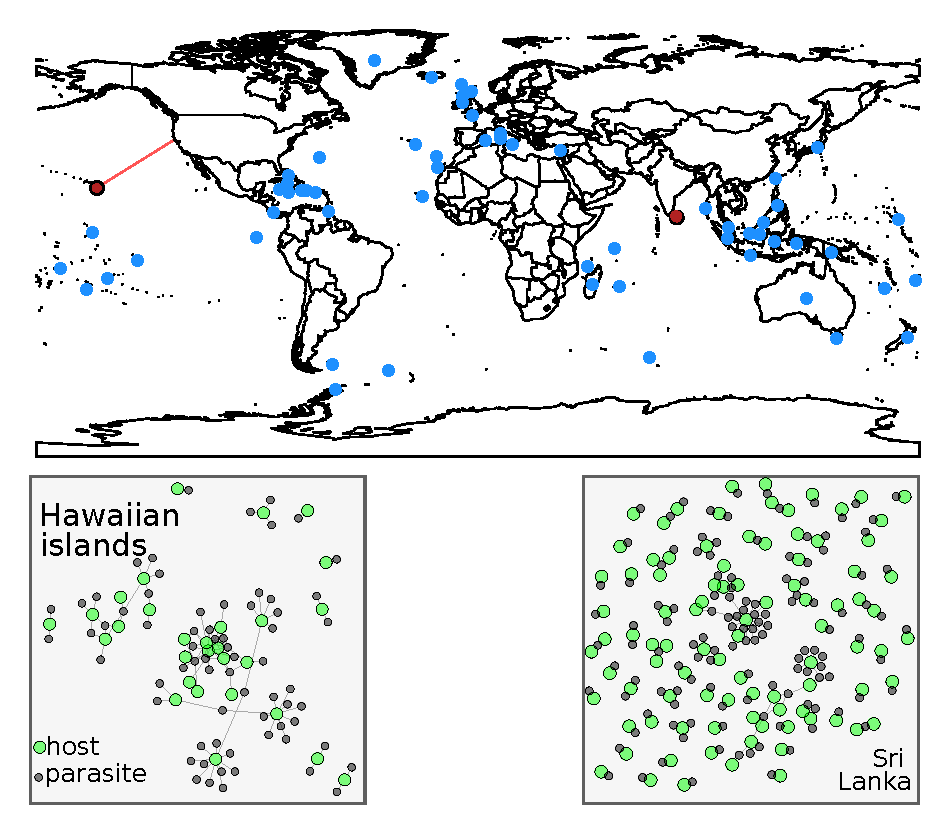
\includegraphics[width=\textwidth]{HelmBiogeog/Figures/conceptual/concept.pdf}
    \caption{Both distance to mainland and island area may influence species richness and host-helminth network structure. Islands considered in the analysis are in blue, with two example networks from the Hawaiian islands and Sri Lanka highlighted in red. Hawaii is much smaller and more distant to the mainland, and also has lower species richness relative to Sri Lanka. }
    \label{fig:concept}
  \end{center}
\end{figure}

\clearpage


\begin{figure}[h!]
  \centering
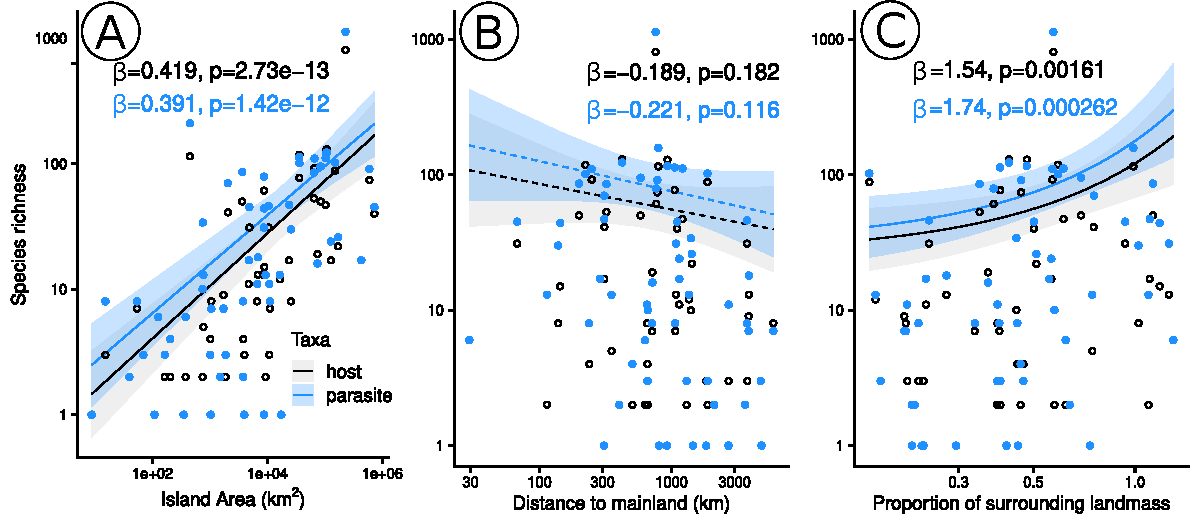
\includegraphics[width=\linewidth]{HelmBiogeog/Figures/NB_MarginalPlots_Wide.pdf}
  \caption{Traditional island biogeography theory relates species richness to the distance to the mainland (i.e., isolation) and island area. We detect a significant positive effect of island area on both helminth parasite and host richness (A), but found no significant effect of isolation as measured by distance to mainland (B). When measuring island isolation through surrounding landmass proportion, we did detect a weak but significant positive effect of island connectivity on both helminth and host richness (C). Plotted lines represent fitted relationships from a negative binomial multivariate regression model, assuming mean values of non-focal predictor variables. Significant relationships represented as solid lines; shaded regions represent 95\% confidence intervals.}
  \label{fig:islandBG}
\end{figure}

\clearpage

\begin{figure}[h!]
  \begin{center}
    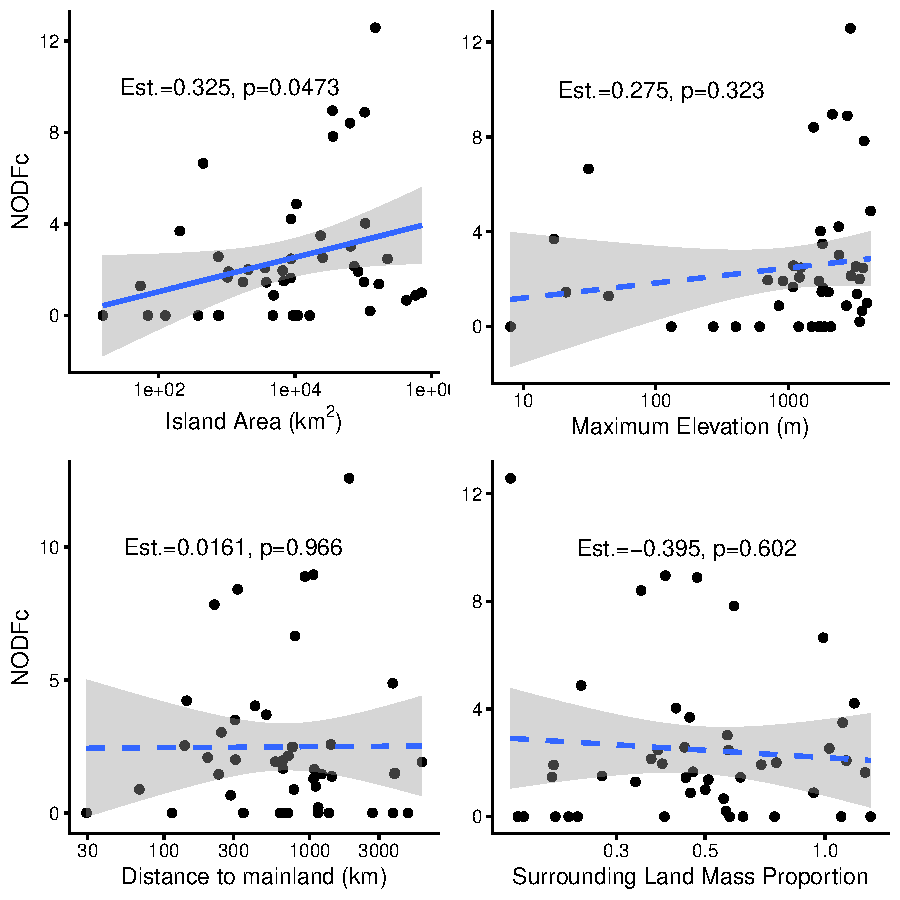
\includegraphics{HelmBiogeog/Figures/NODFc_plots.pdf}
    \caption{In addition to impacting network size, island area was positively related to $NODF_c$ such that larger islands were tended to be more nested on average (top left). In contrast, neither island elevation (top right) nor measures of island isolation including distance from the mainland (bottom left) or SLMP (bottom right) were significantly related to interaction nestedness within island networks.} %GF: Still need to add labels as well as fix cut off island area x-axis
    \label{fig:networkBG}
  \end{center}
\end{figure}

\clearpage


\begin{figure}[h!]
  \begin{center}
    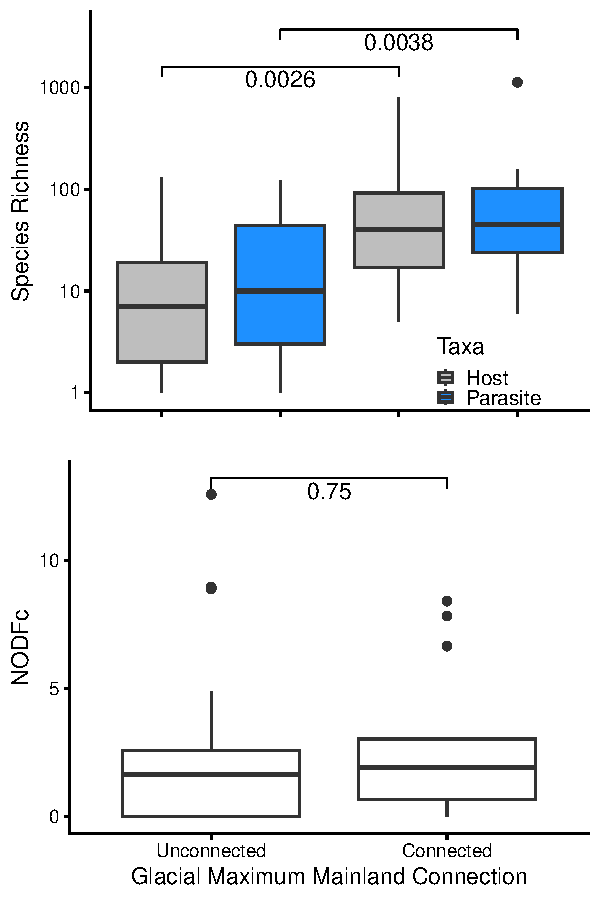
\includegraphics{HelmBiogeog/Figures/GMCC_NODFc_boxplots.pdf}
    \caption{Islands with a terrestrial connection to the mainland during the most recent glacial maximum have significantly higher host and helminth parasite diversity (top), but exhibit no significant differences in network nestedness. Comparison labels indicate p-values from a pairwise Wilcoxon test.}
    \label{fig:GMMC}
  \end{center}
\end{figure}













%--- Supplement ---

\clearpage

\section*{Supplemental Material}

\title{Island biogeography of host-helminth interaction networks}

\author[a,*]{Grant Foster}
\author[a,b]{Tad A Dallas}
% TAD: I don't think this will actually work, so maybe just write it out instead of trying to format it like main text. 

\affil[a]{Department of Biological Sciences, University of South Carolina, SC 29208, USA}
\affil[b]{Center for the Ecology of Infectious Diseases, University of Georgia, Athens, GA, 30602}


\renewcommand\Authands{ and }
\date{ \small *Corresponding author: grant.t.foster500@gmail.com}



\beginsupplement



\subsubsection*{The relationship between network size and nestedness}

Disentangling species richness (the sum of host and parasite richness) from nestedness is difficult, and many nestedness measures scale with species richness (Figure \ref{fig:richnessEffect}). Comparisons of properties across networks of different sizes is a non-trivial problem, and one potential solution is the implementation of a null modeling approach. In our case, we repeatedly shuffle links between hosts and helminths in each network, while maintaining both parasite host range (i.e., the number of host species a given parasite infects), and parasite species richness (i.e., the number of parasite species a host is infected by). For each network, we produced 1000 randomized networks, creating a distribution of spectral radii. Using these null distributions, we calculated $z$-scores, which measure the degree of divergence of the empirical network from the randomized null networks. Below, we present the correlations between alternative measures of network nestedness ($\eta$\citep{jonhson2013factors}, spectral radius, NODF, and $NODF_c$) as well as z-transformed versions of NODF and spectral radius. Nestedness as measured by $\eta$ was not standardized, as null model randomization for this measure is difficult, as randomized networks maintaining aspects of the degree distribution of host and parasite species will result in the same $\eta$ value as the empirical network. 

We find a significant correlation between the log-scale number of species within a network and all of the most common measures of network nestedness. However, as shown by \citet{song2017some}, $NODF_c$ is unrelated to network size or connectance across large sets of randomly generated networks. The relationship we observe across island networks may therefore reflect covariance with island area rather than a direct effect of network size on nestedness. Island area is positively associated with both network size \ref{fig:islandBG} and network nestedness \ref{fig:nestMod}, suggesting that area may act as a shared underlying driver that confounds the apparent association between network size and nestedness. As such, using metric sensitive to network size may give conflicting results. \ref{fig:Spectral.z_Results} illustrates that when using z-standardized NODF as our measure of interaction nestedness, we see the opposite relationship between island area and nestedness as with our $NODF_c$ metric, as well as relationships with elevational range and SLMP. In contrast, measuring interaction nestedness by the z-standardized spectral radius of a given graph yields qualitatively similar results to $NODF_c$ \ref{fig:Spectral.z_Results}.  

\begin{figure}[h!]
  \begin{center}
    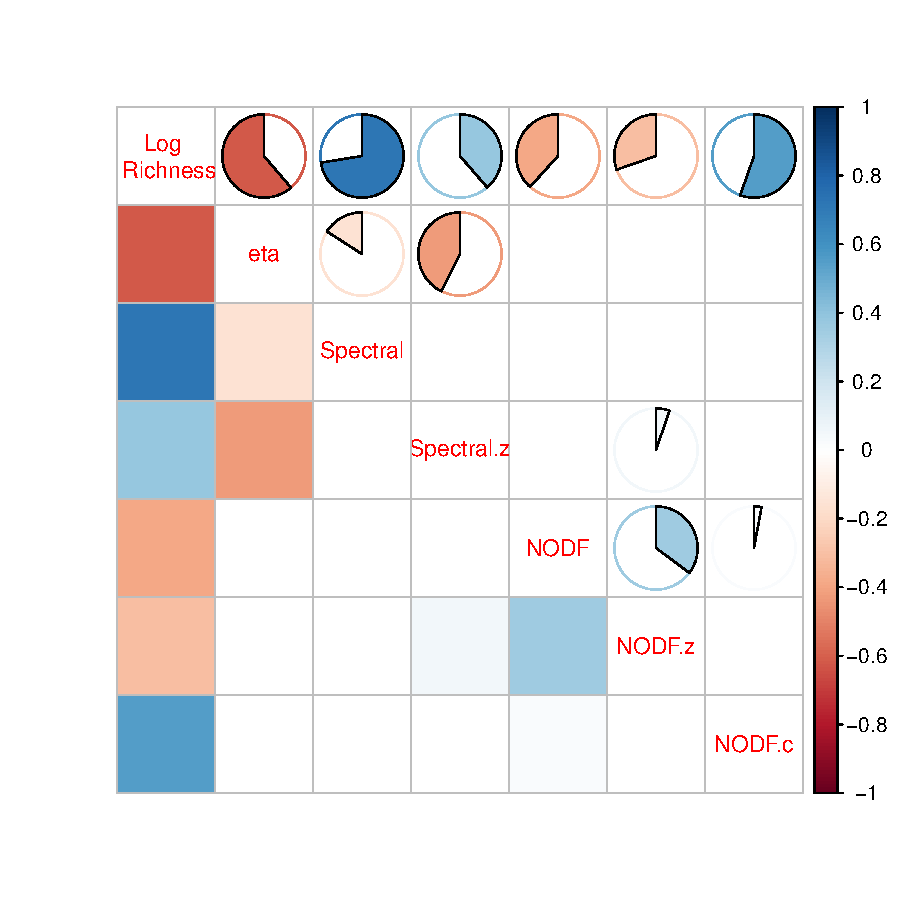
\includegraphics[width=\textwidth]{HelmBiogeog/Figures/Netsize_corplot.pdf}
    \caption{Correlogram visualizing Pearson's correlation coefficients between network size (log species richness) and alternative measures of network nestedness in our data. Shaded squares represent significant correlations (p-value $<0.05$). All measures of nestedness ($\eta$\citep{jonhson2013factors}, spectral radius, and NODF, as well as z-scores of the latter two based on null randomizations) are significantly correlated with network size in our dataset}
    \label{fig:richnessEffect}
  \end{center}
\end{figure}


\begin{figure}[h!]
  \begin{center}
    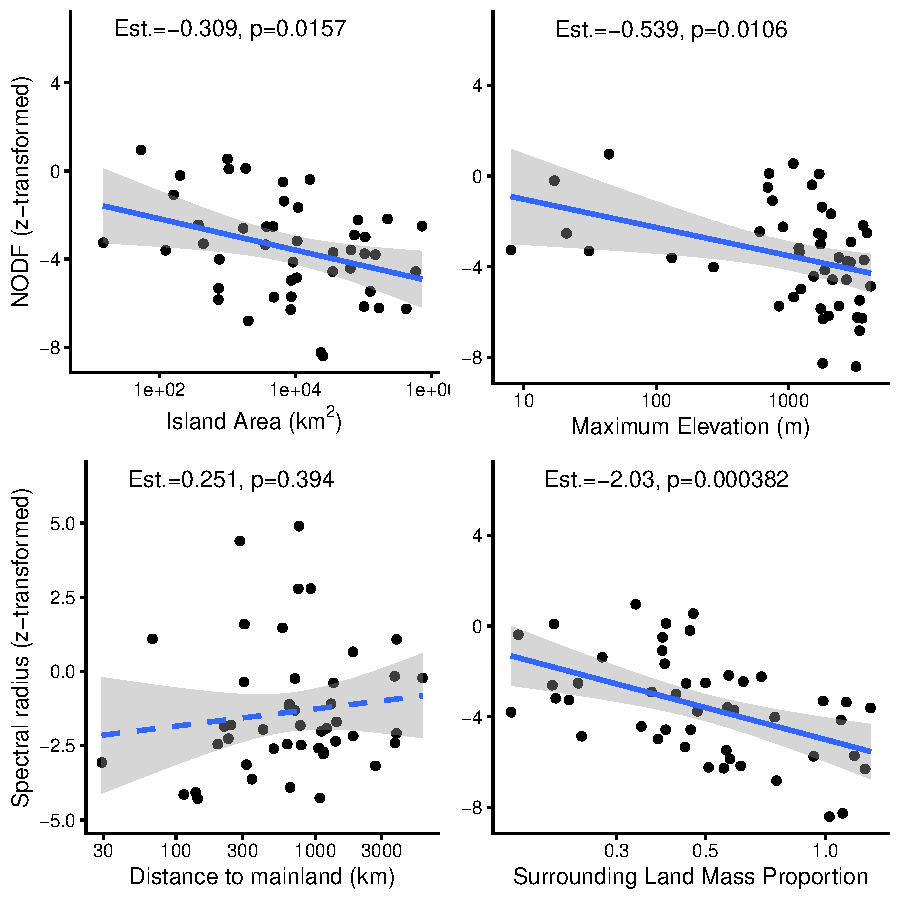
\includegraphics[width=\textwidth]{HelmBiogeog/Figures/NODF.z_Plots_Supplement.pdf}
    \caption{Recreation of Figure \ref{fig:networkBG} of the main text using z-transformed NODF as our nestedness metric of comparison. Despite null modeling approaches, this metric may still be sensitive to network size, and this gives conflicting results to those observed in $NODF_c$. }
    \label{fig:NODF.z_Results}
  \end{center}
\end{figure}

\clearpage

\begin{figure}[h!]
  \begin{center}
    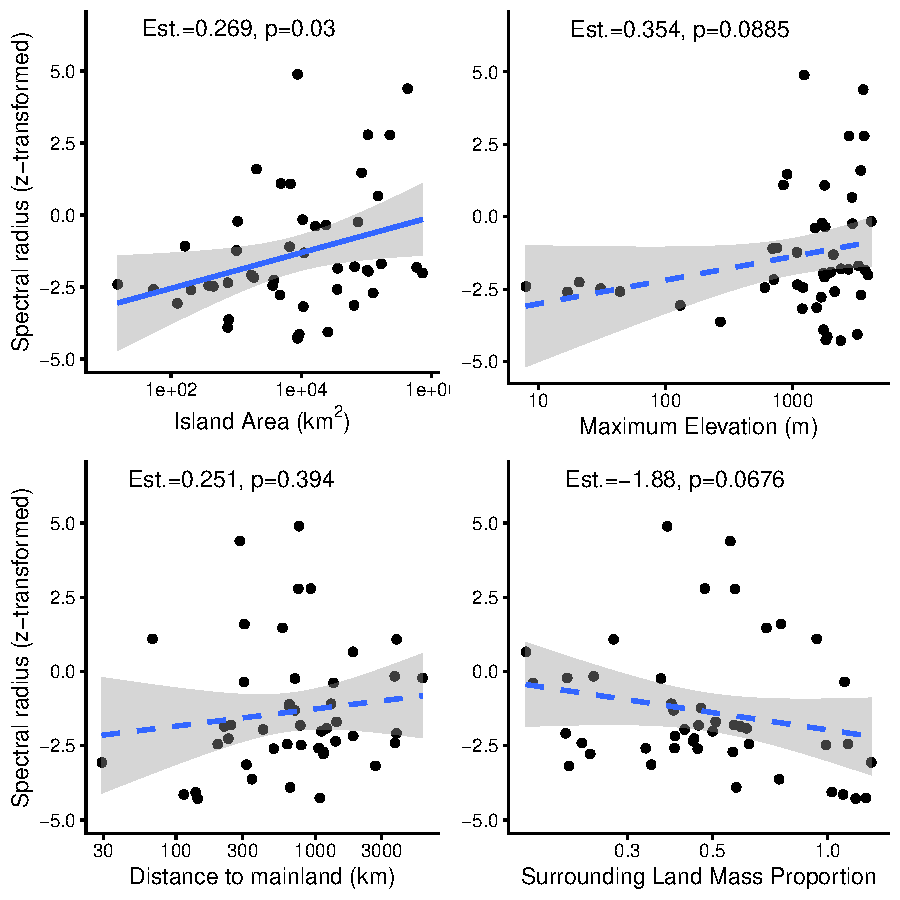
\includegraphics[width=\textwidth]{HelmBiogeog/Figures/Spectral.z_Plots_Supplement.pdf}
    \caption{Recreation of Figure \ref{fig:networkBG} of the main text using z-transformed spectral radius as our nestedness metric of comparison. In contrast to z-standardized NODF, spectral radius yields qualitatively similiar results to $NODF_c$ after z-transformation.}
    \label{fig:Spectral.z_Results}
  \end{center}
\end{figure}


\subsubsection*{Statistical Analysis}

In the main text, we use a negative binomial modeling multivariate regression approach to model the effects of island characteristics on species diversity. This approach greatly minimizes residual deviance compared to both Poisson and Quasi-Poisson GLMs \ref{tab:host_div_deviance}. Models incorporating island area and isolation as measured by SLMP yielded lowest AIC values, and as such are presented in the main text. 

\begin{table}[ht]
\centering
\caption{Model deviance diagnostics for host diversity models.}
\label{tab:host_div_deviance}
\begin{tabular}{lrrrr}
\hline
Model & Residual deviance & Residual df & AIC & Deviance/df \\
\hline
Poisson: Area + SLMP & 5621.91 & 55 & 5873.20 & 102.22 \\
Quasi-Poisson: Area + SLMP & 3497.06 & 55 & -- & 63.58 \\
Negative binomial: Area + Distance & 65.10 & 55 & 488.86 & 1.18 \\
Negative binomial: Area + SLMP & 63.90 & 55 & 481.30 & 1.16 \\
Negative binomial: Elevation + Distance & 69.24 & 55 & 515.87 & 1.26 \\
Negative binomial: Elevation + SLMP & 68.08 & 55 & 509.48 & 1.24 \\
\hline
\end{tabular}
\end{table}


Below, we report model diagnostic plots for the three models in the main text which show significant relationships between island characteristics and network properties. 

\begin{figure}[h!]
  \begin{center}
    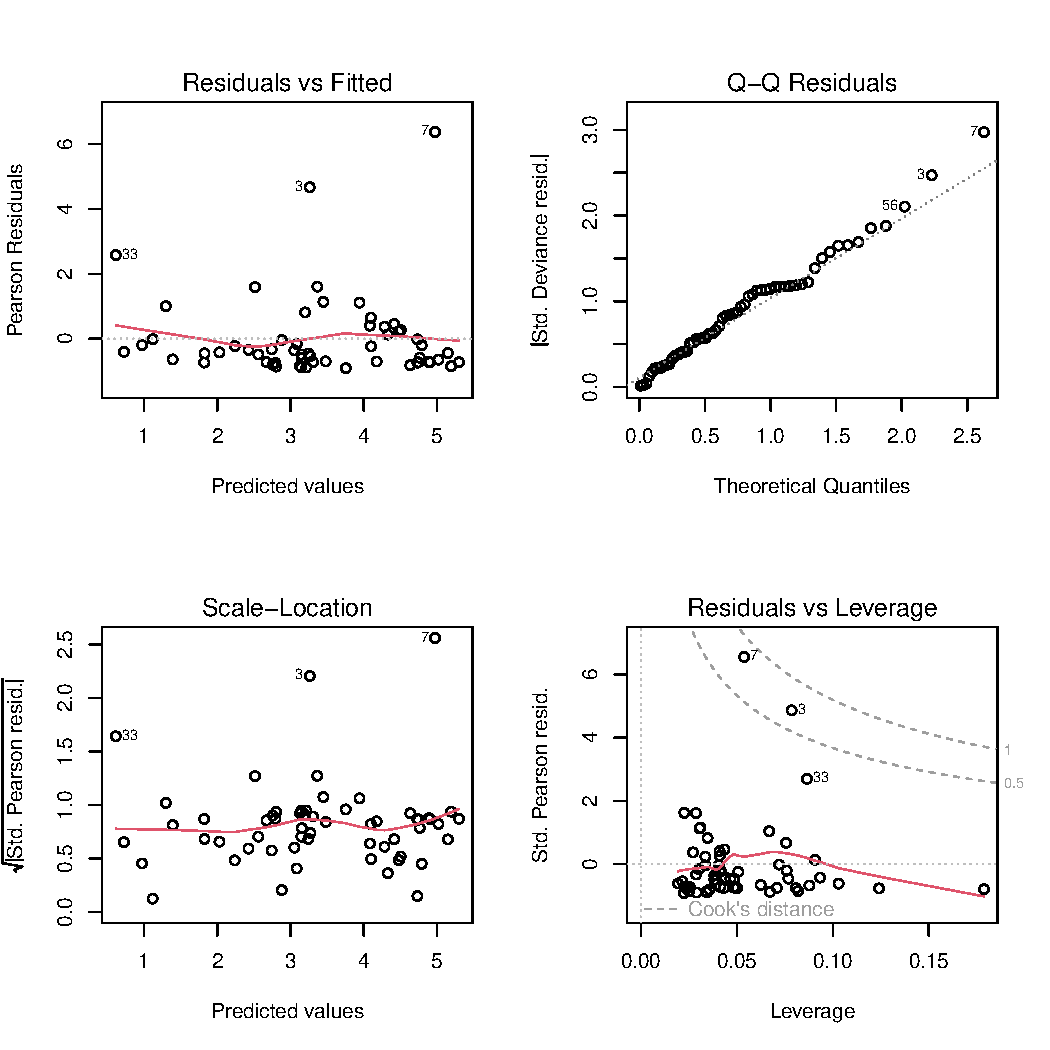
\includegraphics[width=\textwidth]{HelmBiogeog/Figures/ParDiv_diagnostics.pdf}
    \caption{Model diagnostics plots for our negative binomial model of \textbf{parasite richness} across islands, including residual vs fitted values (top left), Q-Q plot (top right), scale-location (bottom left), and residual vs leverage plot (bottom right), with dotted lines representing Cook's distance contours of 0.5 and 1, respectively. }
    \label{fig:parDivdiagnostics}
  \end{center}
\end{figure}

\begin{figure}[h!]
  \begin{center}
    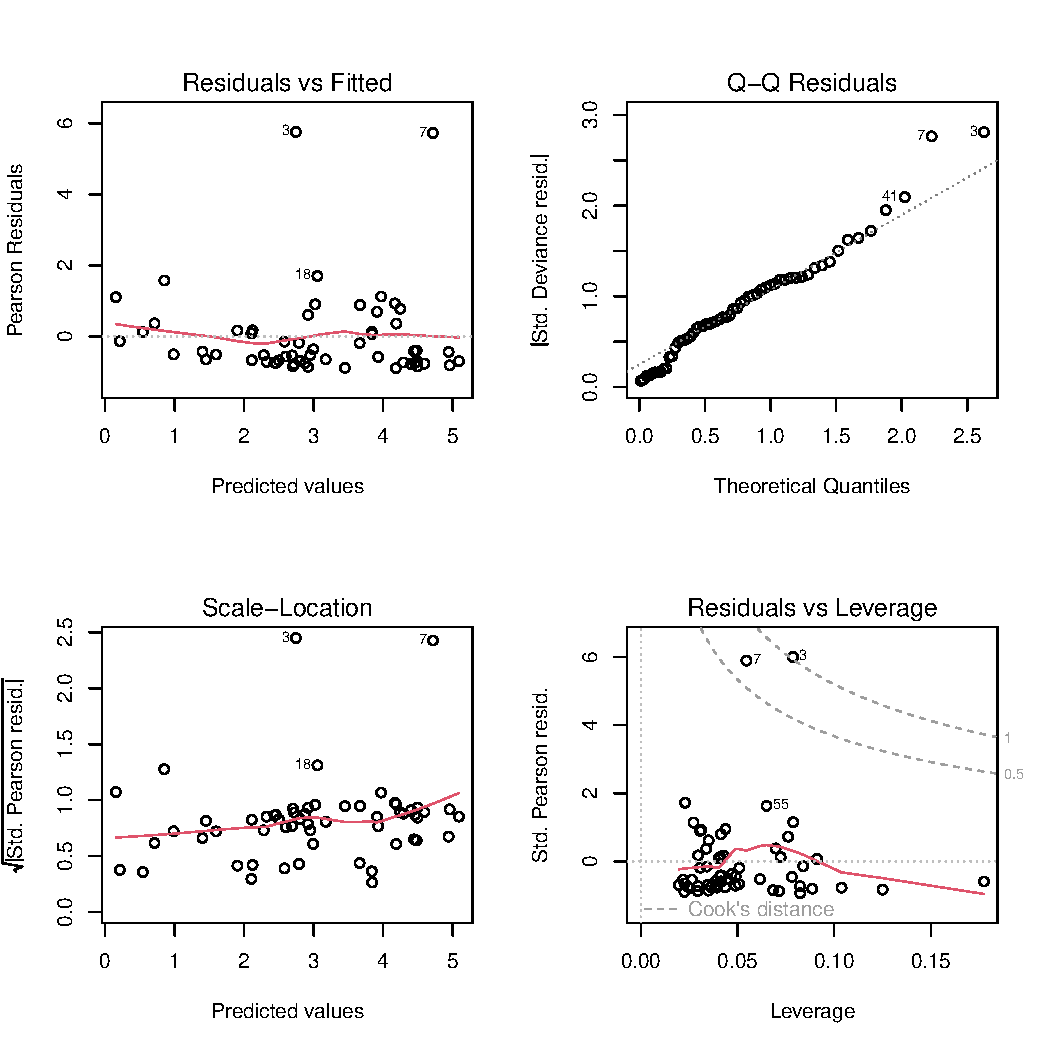
\includegraphics[width=\textwidth]{HelmBiogeog/Figures/HostDiv_diagnostics.pdf}
    \caption{Model diagnostics plots for our negative binomial model of \textbf{host richness} across islands, including residual vs fitted values (top left), Q-Q plot (top right), scale-location (bottom left), and residual vs leverage plot (bottom right), with dotted lines representing Cook's distance contours of 0.5 and 1, respectively. }
    \label{fig:hostDivdiagnostics}
  \end{center}
\end{figure}

\begin{figure}[h!]
  \begin{center}
    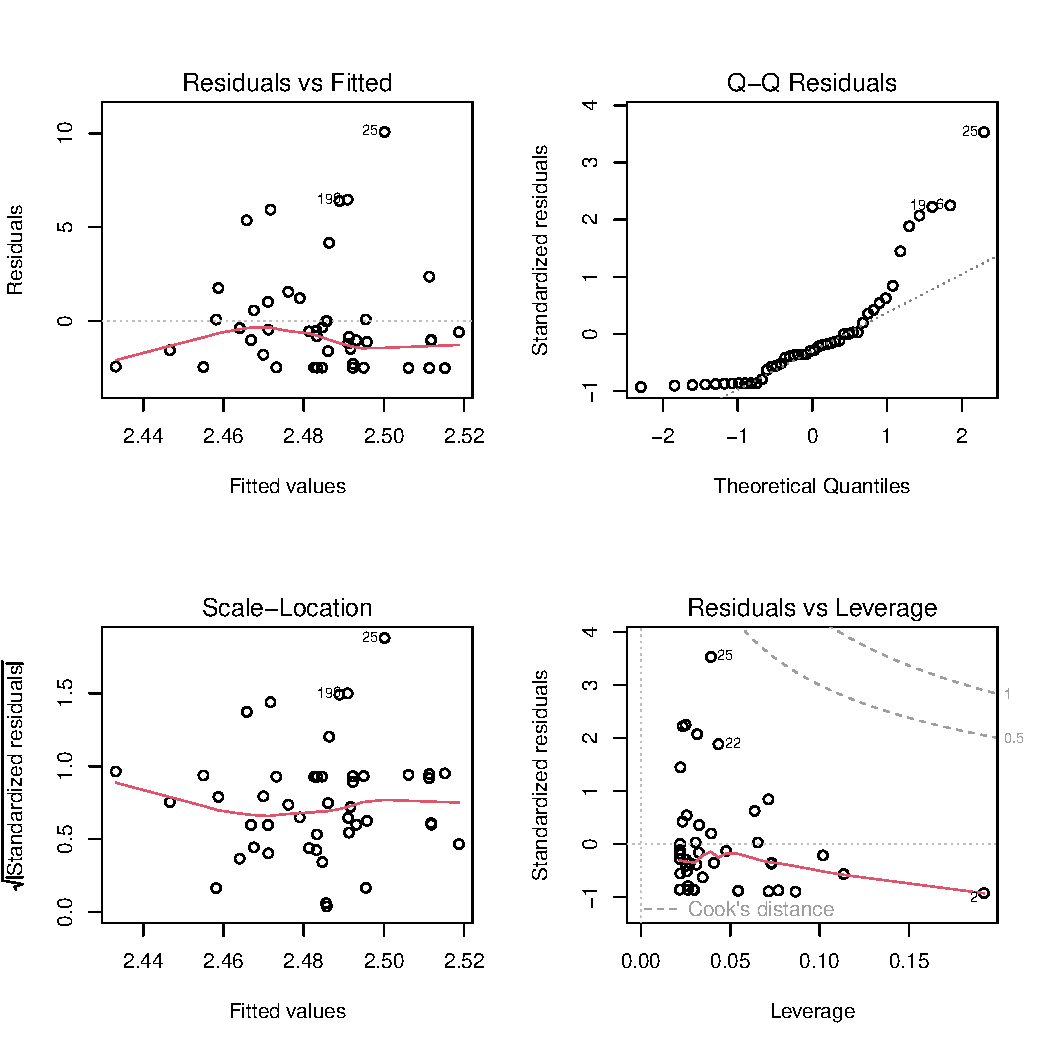
\includegraphics[width=\textwidth]{HelmBiogeog/Figures/NODFc_Distance_diagnostics.pdf}
    \caption{Model diagnostics plots for our generalized linear model of \textbf{network nestedness ($NODF_c$)} across islands, including residual vs fitted values (top left), Q-Q plot (top right), scale-location (bottom left), and residual vs leverage plot (bottom right), with dotted lines representing Cook's distance contours of 0.5 and 1, respectively. }
    \label{fig:nodfcdiagnostics}
  \end{center}
\end{figure}

\clearpage\\

\subsubsection*{The relationship between nestedness and modularity}

We don't consider modularity in the main text, but we explore it here for fun, as it is closely related to nestedness. Cite arxiv paper and Fortuna 2010 \citep{fortuna2010nestedness} and say that they are like...the same thing.


GF: How necessary do you think this addition is? Can add it back in if you think so, but would need to recalculate on our new network sets. 
\clearpage
                                                                  


\addtocontents{toc}{\protect\vskip-20pt}
\chapter[Structural Changes in Mutualistic Networks under Global Anthropogenic Pressure]{Structural Changes in Mutualistic Networks under Global Anthropogenic Pressure}   

\section*{\textbf{\underline{Abstract}}}
Plant-animal transport mutualisms, such as seed dispersal and pollination, represent a diverse suite of interactions that impact the function and dynamics of many ecological communities. Network representations of these interactions exhibit a wide range of structural properties (e.g. nestedness, modularity) that ultimately mediate emergent properties of ecological relevance (e.g. stability, resilience, robustness to secondary extinction). Understanding how these structural properties are affected by anthropogenic forcing and how they scale up to shape emergent properties is vital for predicting and conserving mutualistic networks in the face of global change. Here, I review the current state of knowledge on how three major classes of anthropogenic impact: shifts in global climate, land use intensification, and human-mediated invasion, affect the structural properties of plant-animal transport mutualism networks. In particular, I synthesize emerging patterns and persistent knowledge gaps in how these drivers alter network structure across systems and scales. Finally, I highlight a series of open questions in the field, the answers to which may help elucidate how these structural shifts scale up to changes in community dynamics, and ultimately improve our ability to predict and conserve mutualistic systems.

\section*{\textbf{\underline{Introduction}}}
\paragraph*{Mutualisms are important to the function of ecosystems}\mbox{}\\ 
The term "mutualism" covers a broad suite of species interactions, many of which are collectively vital to the function of many ecosystems as we currently know them \parencite{boucher1982ecology}, and iconic organismal features such as flowers or fruits are living homages to the mutualisms that they support \parencite{weiblen2015evolutionary}. The flow of resources facilitated by these and other mutualistic interactions can serve key ecological functions, and ultimately provide significant ecosystem services to human communities across the planet. Globally, pollinators may provide as much as \$400 billion annually in agricultural pollination services alone as of 2020 \parencite{porto2020pollination}, and are relied upon by 85\% of extant plant species across the globe \parencite{ollerton2011many}.
    

\paragraph{}
Due to their outsized impact on ecosystem function and services, understanding how mutualistic interactions change in response to perturbation is of great interest. These influential interactions do not happen in a vacuum, and taking a network approach to studying mutualisms can better allow us to understand how mutualisms as a whole affect the structure, function, and resultant services provided by an ecosystem. N	etwork approaches allow us to more clearly understand how perturbations propagate through a system, and have been used to study consumer-resource interactions \parencite{rooney2012integrating}, nutrient cycles, \parencite{christian1996nitrogen}, host-parasite interactions, \parencite{dallas2015co}, and mutualistic interactions \parencite{vanbergen2017network, rohr2014structural}. Together, these approaches have enhanced the ability to predict how diverse communities may respond to environmental change. In order to understand how communities of interacting species may change in the face of growing anthropogenic forcing, it is vital to understand how human-induced changes tend to affect the structure and function of mutualistic networks. 

%There have been massive changes in mutualistic networks
\paragraph*{}
Global ecosystems are subject to anthropogenically driven changes at increasing rates, and as a result, so are the mutualistic interaction networks that occur within them. Structural changes in mutualistic networks can be driven by a diverse set of drivers, including shifting climates, urbanization and land use changes, and invasion of non-native species. Here, I aim to characterize the current state of understanding about the ways these diverse drivers affect the structural properties of two major classes of plant-animal transportation mutualisms \parencite{bronsteinmutualism1}: seed dispersal and pollination networks, as well as how we can leverage our knowledge of these patterns to better understand, predict, and conserve these critical natural systems. 


% TD: you use 'we' 30 times. It's a bit informal to use this, but I also don't want to tell you to use the passive voice too much. Maybe change some of them, because I'm already picking up on it at this point and I think a reviewer will too. 

\paragraph*{Emergent Properties of Mutualist Networks}\mbox{}\\ 
The structure of relationships within mutualistic systems can generate dynamic system-level behavior, including several emergent properties useful for understanding how mutualistic systems may respond to perturbation (Figure \ref{fig:ConceptDraft}). These include properties describing how mutualistic networks behave around equilibrial states, a number of which can be estimated through eigenanalysis of the Jacobian matrix representing mutualistic communities at equilibrium. Both local stability (the tendency of the system to dampen small perturbations from equilibrium) \parencite{valdovinos2019mutualistic, okuyama2008network}, as well as resilience (here, the speed at which the system returns to equilibrium after perturbation) \parencite{thebault2010stability, suweis2013emergence}, are important for predicting how mutualistic networks respond to anthropogenic change. Other properties include the size of the feasibility domain, the range of parameter values that permits non-zero equilibrium abundances for all species in a community \parencite{saavedra2016nested, grilli2017feasibility, wang2023interspecific}. This property, sometimes referred to as structural stability, defines the safe operational space within which all species can persist \parencite{bascompte2022resilience}. Given an existing network structure, the extent to which disturbances spread widely or remain confined to local subsets of species \parencite{martins2024propagation, suweis2015effect} is yet another emergent feature of interest in the context of anthropogenic change, and is closely related to the structural property of modularity. 


\paragraph{}
These metrics collectively provide important insights into how existing network structure may mediate the impact of perturbation, but we are also interested in how networks may be sensitive to changes to their existing structure. By definition, mutualistic partners improve one another's fitness; if the magnitude of benefit scales in some way with population size \parencite{valdovinos2019mutualistic}, positive feedbacks between partnered populations or threshold responses \parencite{hale2021ecological} may occur. Disrupting these positive feedbacks of networks can facilitate critical transitions, and structural properties of networks can be important for determining behavior at the critical boundary or determining how robust a network is to loss of certain nodes or links \parencite{van2021facultative}. For example, simulated plant-pollinator networks with greater connectance are more likely to undergo large critical transitions as extinctions occur, undergoing larger community-level breakdowns instead of many small breakdowns \parencite{lever2014sudden}. Positive feedbacks may also induce hysteretic effects crossing the critical transition boundary; that is community assembly and disassembly processes may often be non-symmetric in mutualistic systems, with the outcome depending on precursor system states \parencite{cai2020mutualistic}. Understanding how these processes occur and are influenced by network structural properties is vital for both prediction and conservation of mutualistic systems.


\paragraph*{The Importance of Structural Properties}\mbox{}\\ 
%Structural features affect emergent ones
Many of these aforementioned emergent properties of interest (stability, resilience, hysteresis, etc.) are heavily impacted by network structural properties \parencite{landi2018complexity}. A significant body of existing literature has been devoted to interrogating relationships between the structural properties and emergent properties of species interaction networks, though at times with counterintuitive results. For example, network modularity (the property of having more connections within smaller subunits of a network than between them) tends to reduce the propagation of direct or indirect perturbations through a mutualistic system \parencite{thebault2010stability, okuyama2008network}. Invasion by non-native generalist species increases connectance and decreases modularity of some networks, potentially leading to broader or faster propagation of disturbances in the face of a changing environment \parencite{fricke2020accelerating, vollstadt2022plant, martins2024propagation}.  Because of their important and often complex effects on emergent properties, understanding how network structural properties tend to change in response to anthropogenic forcing is vital for prediction and management of mutualistic systems. 

%How structure -> Emergent is complicated
\paragraph*{} 
Structural properties often have nuanced effects on multiple emergent properties, making it important to identify which emergent properties are most relevant in a given context. For example, one widely observed property of mutualistic networks is nestedness, in which specialist species with few interaction partners tend to interact with generalist species that have many partners, effectively embedding specialist interactions within a broader, generalist core \parencite{bascompte2003nested, bascompte2006asymmetric, thebault2010stability}. As nestedness increases, the overall robustness of the system to species loss may increase due to functional redundancy, while simultaneously making the final breakdown of the system more dramatic (increasing magnitude of critical transitions) \parencite{bascompte2022resilience}. The nestedness of strong interactions tends to increase the size of a mutualistic system's feasibility domain \parencite{saavedra2016nested}, yet decrease its stability at equilibrium \parencite{allesina2012stability}. However, even if more nested mutualistic networks are less stable, they may lead to higher overall community abundance, an effect stronger in systems characterized by abundant but weak mutualisms \parencite{suweis2013emergence}. Robert May first pointed out in 1973 the ``paradox of complex interactions", where, under a Lotka-Volterra style modeling framework, larger species assemblages with many strong and randomly assigned species interactions lead to correspondingly smaller feasible domains of community stability \parencite{may1973stability}, a pattern that tends to be even more pronounced in mutualistic systems \parencite{allesina2012stability, saavedra2016nested}.  In reality, however, interactions are not randomly assigned within a community, and empirically observed suites of mutualistic interactions often tend to favor stability in practice, though to varying degrees \parencite{thebault2010stability, grilli2017feasibility}. How structural properties translate into emergent ones may be further complicated by plasticity in species interaction preferences \parencite{corro2021annual} or the degree of nodes' dependence on mutualisms \parencite{van2021facultative}. Valdovinos et al. (2016) found that accounting for potential adaptive foraging behaviors reversed the effects of nestedness and connectance on species persistence times \parencite{valdovinos2016niche}. In general, the relationship between structural and emergent properties is complicated and can lead to counterintuitive results \parencite{landi2018complexity}.

\paragraph*{} %How do structural features arise? 
The mechanisms under which emergent properties arise in networks across a landscape still warrant further investigation, especially in the context of mutualistic systems. In food webs, Borrelli et al. (2015) found that stabilizing motifs were overrepresented relative to null expectations across a diverse set of 50 networks, potentially indicating the presence of stabilizing processes present across landscape scales \parencite{borrelli2015selection}. This is supported by prior work looking at the constancy of network structural properties across scales in both trophic \parencite{fahimipour2014dynamics} and host-parasite \parencite{dallas2018compositional} networks, even as individual species turn over across space. The conservation of network properties despite species turnover may indicate that separate assembly mechanisms operate at the level of interaction networks and species assemblages per se \parencite{petanidou2008long, dupont2009spatio, burkle2011future, dehling2020similar, ten2024latitudinal}. One potential set of mechanisms acting on network structure may be non-Darwinian selection processes \parencite{saravia2022ecological}, where more stable networks endure longer through time as less stable networks break down, a potential phenomenon supported by theoretical modeling work \parencite{cai2020mutualistic}. However, one must be cautious in interpreting the prevalence of stabilizing structural properties as evidence for these processes; Saravia et al. (2022) found little difference between realized local networks and random draws from the regional metaweb in trophic networks \parencite{saravia2022ecological}, emphasizing the importance of proper null models in the context of network structure \parencite{maynard2018network, pellissier2018comparing}. Additionally, while different structural measures capture different aspects of network topology, they are seldom independent, a feature well-appreciated in food webs \parencite{vermaat2009major}. Understanding how structural properties covary is another reason null model approaches are important and looking at joint properties may be useful \parencite{fortuna2010nestedness, poisot2014ecological, pellissier2018comparing, dormann2017}. 



%Network properties may also influence individual species fitness components predictably, according to their traits, with even the fitness benefit conveyed by given interactions depending on community structure (ex. Specialists in nested communities had higher closeness centrality. 



\paragraph*{Widely Observed Structural Properties of Mutualistic Networks}\mbox{}\\ 
%Emp Nets are Nested
There are a number of properties pervasive in empirically observed frugivory and floral visitation networks. Empirical networks often exhibit high degrees of interaction nestedness \parencite{fortuna2006habitat, bascompte2006asymmetric}, a product of the asymmetric specialization widely observed in both seed-dispersal \parencite{yohe2025frugivore, schleuning2014loss} and floral visitor networks \parencite{bascompte2003nested}. This feature tends to increase the strength of highly connected nodes, often resulting in long-tailed degree distributions. Especially in pollination systems there may be trade-offs in specialization stemming from this pervasive interaction asymmetry; \parencite{arceo2020plant} found that a plant's degree specialism was positively related to heterospecific pollen delivery, likely due to associations with generalist pollinators \parencite{arceo2020plant}. Nestedness may increase positive indirect interactions within guilds, ultimately increasing the potential diversity of species a community can support \parencite{bascompte2003nested, guimaraes2017indirect}. It also can reduce effective interspecific competition, increasing equilibrial species richness \parencite{bastolla2009architecture}, a pattern potentially observed in empirical networks \parencite{Gonzales2015macroecology}. 

%Emp Nets are Modular
\paragraph*{}
Modularity is another prevalent feature of mutualistic networks, many of which may be separated by functional guilds \parencite{ramos2018modularity} or phylogenetically conserved groups of interaction partners \parencite{Gonzales2015macroecology}. Species with certain traits or within certain taxonomic groups may be more likely to make cross-module connections. Sebasti{\'a}n-Gonz{\'a}lez (2017) found that a small number of highly frugivorous birds and high energy content fruits had higher connectivity both between and within modules \parencite{sebastian2017drivers}. In their study of Peruvian highland pollination networks, Watts et al. (2016) found connector species were likely to be comparatively generalist and taxonomically clustered (\textit{Diptera: Syrphidae} and \textit{Asterales: Asteraceae}). The introduction of a relatively small number of species with higher or lower propensity to establish cross-module connections can fundamentally alter the resultant modularity of a given network \parencite{russo2014patterns}, an idea further explored in the section \textbf{Invasion}.  
%Emp Nets are Sparse? Do I need to talk about this? Ecological networks are generally sparse, a feature that can be a problem for prediction. 
% TD: eh. If the focus was on prediction, I would say sure, but 1 sentence tops should be spent on that, and I'd do it in a section where you talk about how lower-level properties scale to emergent properties (i.e., sparse networks can't really be nested, right?). 


%Emp features may change across space...
\paragraph*{}
Agnostic to changing environments, some evidence shows that network structural properties vary across preexisting environmental or spatial gradients.  In a study of both insect and avian pollination networks across broad latitudinal coverage  Tr{\o}jelsgaard and Olsen (2013) found that modularity was highest at low latitudes whereas nestedness peaked at mid-latitudes \parencite{trojelsgaard2013macroecology}. Across altitudinal gradients, multiple studies have observed an increase in phylogenetic generalism and an associated increase in nestedness and connectance with increasing elevation in plant-pollinator networks \parencite{adedoja2018insect, lara2019beta, classen2020specialization}, though similar evaluations to my knowledge have not been made in frugivory systems. 

%Or climate.
\paragraph*{}
Both the mean and variability of temperature may also play a role in shaping network structural properties; Welti et al. (2015) found that both seed dispersal and floral visitation networks were generally more nested in areas with higher inter-annual temperature variability \parencite{welti2015structure}. Gonz{\'a}lez et al. (2015) found that in mainland plant-hummingbird networks warmer and more stable climates were associated with higher modularity, though these variables had no effect on island networks \parencite{Gonzales2015macroecology}. Both current and past climatic features may have significant effects on network structure \parencite{dalsgaard2013}, further complicating the question of how and at what rate networks may respond to future climatic change. 

\section*{\textbf{\underline{Anthropogenic Change and Mutualistic Network Structure}}}
%Transisition into three drivers sections
While existing environmental conditions have already played a role in shaping mutualistic networks as we know them, human impacts have also drastically altered biotic and abiotic conditions across most of the globe. As natural ecosystems are subject to increasingly severe anthropogenic impacts, so too are the ecological networks that occur within them. Understanding how human-mediated changes affect structural properties and resultant dynamics of mutualistic networks is vital for predicting and conserving species interactions. These changes can occur through several mechanisms, including (1) alterations in community composition, (2) shifts in the probability of interactions occurring, and (3) disruptions to the coevolutionary processes underpinning these networks \parencite{tylianakis2017}. Here, I focus on how three major types of anthropogenic disturbance—climatic shifts, changes in land use, and human-facilitated invasion by non-native species—act through these mechanisms to reshape the structural properties of natural mutualistic networks.
\paragraph*{Climate}\mbox{}\\
Changes in climate can affect mutualistic network structure through a number of mechanisms, including inducing changes in species distributions across time and space, altering species abundances, or altering the physiology of interacting organisms. Many plant-animal mutualisms may only be able to occur during relatively short, yet ecologically important developmental or life history windows. For example, animal pollination can only occur when both the flowering time of the plant and the seasonal activity period of the animal intersect. As climate shifts the timing of these developmental periods, phenological shifts and subsequent mismatches have the potential to occur, altering the strength of mutualistic interactions or even removing them altogether \parencite{zettlemoyer2019phenology, burkle2013plant, teixido2022anthropogenic} . For example, in a forest-prairie floral visitation network Memmott et al. (2007) showed that up to 50\% of floral visitors have reduced overlap between their seasonal activity period and known floral resources over the past century \parencite{memmott2007global}. Link rewiring, in which species form new linkages in response to environmental change, may help alleviate some of the effects of phenological mismatch, but fitness reductions due to reduced phenological overlap with mutualists have been observed empirically \parencite{kudo2019spring, de2023warming}. Corresponding reduction in pollinator fitness have yet to be observed in field systems, though these reductions are likely already occurring in some contexts \parencite{gerard2020global}. These altered interaction probabilities can scale up into altered network structural properties; Encinas-Viso et al. (2012) found in simulated communities that increasing phenological overlap between competitors led to less stable, less nested, and ultimately less speciose communities \parencite{encinas2012phenology}. As climate shifts phenological periods, even if mutualistic interactors remain phenologically coupled, intraguild shifts in species' activity periods (such as overlapping flight or flowering periods) can change competitive interactions with cascading effects through the community \parencite{wang2023interspecific}.
    %Spatial mismatch
    \paragraph*{} 
    Even if mutualistic partners do not become decoupled in time, climate-driven range shifts may also decouple partnerships by reducing spatial overlap. Warming conditions may shift species ranges northward latitudinally or higher in elevation. Differences in features such as generation time and dispersal capacity mean that two mutualistic partners are unlikely to be able to shift their distributions at the same rate. Or, if biotic interactions limit the distributions of some mutualistic species, partners may be unable to shift ranges without commensurate shifts of the distributions of their partners \parencite{warren2014mutualism}. This may be especially salient in the case of seed-dispersal mutualisms, where the ability of plant species to shift their ranges in response to climatic changes may be dependent on their interaction partner \parencite{warren2014mutualism}.

    \paragraph*{}
    While species may shift their distributions or phenology to track preferred environmental conditions, climate change can also alter species abundances, potentially leading to local extirpation. Complete extirpation is not necessary for ecological disruption, however; functional extinction can precede or occur independently of true extirpation when populations become too small to effectively fulfill their roles as mutualists \parencite{costa2018defaunation}. Moreover, mutualistic partners often differ dramatically in their adaptive capacity due to contrasting life histories, such as generation time and population size \parencite{toby2010mutualisms}. For example, the adaptive potential of semelparous insects with annual life cycles differs substantially from that of the long-lived plants they pollinate. Existing work has already shown plant-animal mutualisms are generally weakened by climate change across broad scales \parencite{tylianakis2008global}. Climate-driven extinctions are not necessarily random, and taxonomic or functional biases in abundance changes may have large effects on network properties. Schleuning et al. (2016) found that higher elevation montane mutualism networks were less robust to climate-mediated losses than their lower-elevation counterparts \parencite{schleuning2016ecological}. Limitations to upslope movement have already been shown to reduce population size or extirpate montane species \parencite{freeman2018climate}, potentially putting high elevation mutualistic networks at higher risk of network breakdown. 
    
    %Changes to the phisiology of interactions
    \paragraph*{}
    Changes in environmental conditions may also alter the strength of a given interaction through changes in physiology or interaction preference \parencite{cruz2023mutualisms}, potentially leading to interaction breakdown. Hoover et al. (2012) observed shifts in nectar chemistry as a function of altered pCO$_2$, warming, and nitrogen deposition, which then had downstream effects on experimental pollinator preference and longevity \parencite{hoover2012warming}. Similar changes in pollen quality may also affect nutritional rewards of interactions, altering the fitness or preference of plants or pollinators \parencite{gerard2020global}. These sorts of processes may alter the coevolutionary processes underpinning the development of mutualistic networks, or cause negative fitness consequences in taxa without the plasticity to alter their interaction patterns accordingly. Warming conditions also tend to reduce body size in insects while exerting less predictable effects on the size of plants; this could potentially alter matching of specialized insect feeding morphologies with their plants \parencite{gerard2020global}. These sorts of mismatches can degrade interactions as a function of environment, and understanding how both plant and pollinator traits might shift with changing environments is important for predicting the outcomes even for contemporary interactions \parencite{cruz2023mutualisms}.
    
\paragraph*{Land use}\mbox{}\\
Human-mediated changes in land cover result in large shifts in habitat availability, both in absolute area and spatial distribution. At local scales, the impact of land-use change on network structure depends on the speed, type, and extent of conversion. For example, Theodorou et al. (2017) found previously agricultural areas actually increased in both floral and bee diversity when urbanized, emphasizing the importance of establishing useful bases of comparison \parencite{theodorou2017structure}. As natural areas are fragmented, specialized and rare interactions are lost disproportionally \parencite{aizen2012specialization}, with remaining generalist interactions potentially forming a widespread consistent core of interactions at landscape scales. This loss can be driven by the actual extirpation of specialists from the community itself \parencite{maurer2024landscape}, or by shifting biotic or abiotic contexts reducing the prevalence or efficacy of those interactions \parencite{birkenbach2024land}. In the case of habitat fragmentation, even if overall habitat loss is small the proportion of edge area is increased as existing land-cover types are subdivided. As edge-habitats become more prevalent across the landscape, networks may grow increasingly homogenized as turnover decreases over larger spatial extents, even if local assemblages retain their diversity or structure. 

    
    \paragraph{}
    While land-cover conversion can often have profound impacts on the presence of individual species or interactions at a given site \parencite{theodorou2017structure, schneiberg2020urbanization, maurer2024landscape, birkenbach2024land}, whether these changes scale up into differences in overall network structure may be more context-dependent. For example, a recent paper by Rossi et al. (2025) quantified changes in frugivore networks in disturbed Amazon forest plots, finding that while logging and burning across timescales did reduce richness of both interacting species and links between them, neither had predictable impacts on network structural properties \parencite{rossi2025anthropogenic}. Salazar-Rivera et al. (2020) found that modularity was maintained in periurban frugivory networks compared to undisturbed habitats, only observing a decrease in nestedness  \parencite{salazar2020frugivory}. Network properties at local scales may be maintained if land use changes exert too small of an impact on structural or functional properties of mutualistic assemblages to cause appreciable changes in network structure. However, a lack of difference across disturbance regimes may also be an indication of comparatively strong constraints on potential structural properties that can be realized in a network comprised of a given regional pool of mutualists. 
    
    \paragraph{}
    Observed network structures may help mutualistic communities deal with disturbance, or at least mediate their responses. Fortuna and Bascompte (2006) found that empirically observed networks were more sensitive to simulated small reductions in habitat area, but persisted longer than randomly assembled graphs in the face of severe disturbance, largely due to the large amount of nestedness observed within empirical networks providing functional redundancy \parencite{fortuna2006habitat}. Further empirical observations of how structural properties both mediate the response of mutualistic networks to change, as well as how these changes feed back to alter structural properties are warranted. Even if structural properties are not negatively impacted by altered land use, specific ecosystem services may still be disrupted \parencite{menke2012plant}. For example, Menke et al. (2012) found that frugivory networks along forest edges were more nested and had greater connectance,  but saw an overall decrease in dispersal of large-fruited forest-specialist plants \parencite{menke2012plant}. While helpful for predicting and understanding changes in mutualistic networks, relying on structural properties alone as indicators of network change can mask functionally critical losses. In practice, isolating the effects of land use change from other anthropogenic drivers is often difficult. Areas with large amounts of human-mediated land cover conversion are often subject to increased propagule pressure of nonnative mutualists \parencite{liu2023impact}, which may have their own impacts on network structural properties. 









\paragraph*{Invasion}\mbox{}\\
Human-mediated dispersal has vastly altered species distributions across the globe, and patterns of non-native species invasion can have persistent effects on the structural properties of mutualistic networks. Species with generalist interaction strategies can more easily invade existing ecological networks \parencite{piechnik2008food} and species roles are often conserved between native and invaded ranges \parencite{emer2016species}. Invasive plants are often effectively dispersed by generalist pollinators and seed dispersers \parencite{richardson2000plant}, though in general many successful invaders can also successfully interact with relative specialists in their new range \parencite{stouffer2014exotic}. How the traits of a potential invader relate to the existing community can affect its propensity for invasion; in simulated communities Minoarivelo and Hui (2016) found potential invaders with trait means different from the existing community were more likely to successfully establish \parencite{minoarivelo2016invading}. The generalism or specialism of a potential invader may also be predictive of its effect on network properties given establishment \parencite{russo2014patterns}.

    \paragraph{} %homogenation across scales
    As synanthropic generalist species are introduced into more human-affected habitats, mutualistic assemblages and potentially network structures tend to homogenize across regional scales \parencite{fricke2020accelerating}. Even when homogenization across space is limited in the context of the entire community, persistent "invader complexes" of introduced species that interact with each other may still alter network properties or invasibility \parencite{richardson2000plant, prior2015mutualism, vollstadt2022plant}. Generalist invaders may also have hysteretic effects on networks once well integrated into existing assemblages. In networks where invasive plants have already established, removing them may in fact further alter network structural properties than allowing them to persist \parencite{valdovinos2009structure, aslan2019implications}. Reliance on non-native pollination partners may further exacerbate the effects of other anthropogenic disturbances. Zettlemoyer et al. (2019) found higher phenotypic plasticity and greater phenological shifts in introduced plant species compared to native taxa, potentially further increasing the risk of phenological mismatch between native pollinators and introduced plants they now rely on \parencite{zettlemoyer2019phenology}. Alternatively, while introduced mutualists may provide some direct benefit to native partners, their net effect may remain negative when indirect impacts are considered \parencite{vidal2021variable}. If invading species exert competitive pressure that reduces the abundance of their native intraguild counterparts while simultaneously being less effective at fulfilling mutualistic functions (pollination, protection, etc.), mutualistic networks may collapse functionally even as interactions (e.g. floral visitation, etc.) appear to continue. While tight coevolutionary coupling is seen between some specialist partners \parencite{stebbins1970adaptive}, the widespread generalism exhibited in many animal-plant networks can cause indirect impacts of invaders to play a large role in shaping their eco-evolutionary trajectories \parencite{guimaraes2017indirect, medeiros2018geographic}. Native preferences to associate with introduced mutualists could even cause invasional meltdown of native interactions, a phenomenon exemplified in avian frugivory networks in Hawaii \parencite{VizentinBugoni2021}.


    \paragraph{} %Invasion of generalists leads us to expect changes in invaded network properties, though evidence is mixed in practice 
    If invasion favors generalist species \parencite{piechnik2008food, fricke2020accelerating}, one might expect directional changes in network properties associated with widespread invasion, especially if coupled declines in native mutualists or shifts in their interaction patterns \parencite{aizen2008invasive}. Supergeneralist invaders may significantly increase nestedness by creating cross-module connections \parencite{traveset2014mutualistic}, allowing perturbations to propagate through the network farther and with greater strength. However, invasive species may also provide functional redundancy of potential partners, potentially buffering mutualistic networks against species extinction. Such buffering may not always translate to greater robustness or resilience in the face of broader perturbations. 
    
    \paragraph{}
    In addition to structural properties, emergent properties such as robustness or resilience may be important for predicting the invasibility of a given network \parencite{minoarivelo2016invading}. The presence of invasive mutualists can modify how networks respond to perturbation, potentially altering the severity or likelihood of coextinction cascades. By simulating secondary extinction cascades in invaded or uninvaded empirical networks, Vanbergen et al. (2017) found that coextinctions were less likely in disturbed networks due to functional redundancy of partners \parencite{vanbergen2017network}. However, given that an initial coextinction event occurred, the risk of a cascading collapse was actually higher in these networks, highlighting how expectations about how invasion may impact short- and long-term responses to change differently in some scenarios. 
    
    \paragraph{}
    Expectations for how structural properties translate into emergent properties may be very different depending on the strength and structure of competition within the community \parencite{pascual2017mutualism, wang2023interspecific}. In addition to global homogenization of interactions across scales, Fricke and Svenning (2020) found that more highly-invaded frugivory networks had higher connectance and lower modularity \parencite{fricke2020accelerating}. Some evidence exists that the increasing prevalence of synanthropic generalists in some pollinator communities increases interaction evenness \parencite{schneiberg2020urbanization} or nestedness \parencite{bartomeus2008contrasting}, though the exact pattern of this may depend on factors such as pollination syndrome or local pollinator communities. Vanbergen et al. (2017) also found that disturbed pollination networks were larger, but actually lower in connectance and nestedness \parencite{vanbergen2017network}. Even further complicating expectations, numerous other studies have also observed little to no predictable impact of invasion on overall network properties such as nestedness or modularity \parencite{stouffer2014exotic, parra2021impacts}, even when considering invasion of hypergeneralist plant species \parencite{vila2009invasive}. Further investigation into the processes maintaining network properties despite significant node-level changes is needed to fully synthesize these variable results across systems. 

\section*{\textbf{\underline{Additional Considerations}}}
\paragraph*{The Role of Rewiring}\mbox{}\\
Ecological networks are not static through time or space. While links between species may erode through time in response to changing environments, new links may form as well, a process known as link rewiring. This phenomenon is an important consideration when assessing how mutualistic networks may respond to anthropogenic pressures. While it remains essential to account for processes that erode existing interactions (e.g., phenological mismatches, species extinctions, etc.), failing to account for potential rewiring may lead us to overestimate their effects \parencite{vizentin2020including}. However, despite recent conceptual advances in understanding the rules and constraints that govern rewiring \parencite{corlett2011frugivore, fuzessy2024navigating}, in practice it is often unclear how networks will rewire until they are perturbed, and they may at times fail to rewire as strongly as expected \parencite{leimberger2023plant}. Leveraging predictive approaches can be potentially powerful in this context in order to better understand how networks may respond to change \parencite{eklof2013dimensionality, vizentin2020including, strydom2021roadmap, strydom2023graph, nunes2024estimated}, but to date there are relatively few case studies looking at how networks change through time (though see \parencite{burkle2013plant, olesen2011strong, leimberger2023plant, petanidou2008long}). This gap has been long-acknowledged in the literature \parencite{bascompte2007plant}, but due to the logistical challenges and significant resource requirements of resampling interactions at a given site regularly it is one that we have been slow to fill as a scientific community. From the evidence that does exist, species traits or position within a network may be predictive of their persistence \parencite{burkle2013plant} or rewiring \parencite{sandor2024spatial}.

\paragraph{}
In some cases, phylogenetic conservation of traits or interaction preference may be useful for determining which species may be interacting in present assemblages, as well as which interactions may occur between novel sets of species. This approach has been applied in modern systems \parencite{VizentinBugoni2021} and used to gain insight into paleoecological systems of interacting mutualists \parencite{Braga21}. In other systems, however, phylogenetic relatedness may explain less variation in interactions than directly measured traits \parencite{rafferty2013}. Machine learning approaches can help overcome the problem of predicting potential species interactions as well as potentially identify traits associated with rewiring potential \parencite{pichler2020machine, foster2026comparing}, though care needs to be taken in applying many of these approaches to notoriously sparse ecological data \parencite{poisot2023guidelines}.

\paragraph{}
Species' capacity to rewire may be an otherwise hidden or underappreciated potential of functional redundancy, and affinity-based rewiring has been shown to maintain network properties and stability in theoretical systems \parencite{sheykhali2020robustness}. There are also new exciting avenues for measuring the rate and scale of rewiring as well, with potential for application in ecological systems \parencite{han2019measuring}. However, it is also important to emphasize that mutualistic interactions are not the only relationships being affected by global change. Competitive and trophic interactions are also likely to be affected by anthropogenic drivers, potentially complicating the picture of the emergent outcomes of rewiring. Furthermore, shifts in environmentally-mediated interaction strengths can fundamentally alter the dynamics of a network, even without changing its overall structure.  Mechanisms to maintain mutualisms may be developed on coevolutionary timescales, and species may not be able to alter interaction patterns to reflect current fitness benefits \parencite{toby2010mutualisms}. However, this is not always true; flexibility in interaction preferences has been observed across numerous pollinator \parencite{moran2022flexible} and frugivore taxa \parencite{nowak2013specialist}, and adaptive foraging may help ameliorate the negative impacts of environmental change in some animal taxa \parencite{valdovinos2016niche}. 

% TD: damn this is a long section that seems almost tangential to the main thesis/point of the review. Maybe it's not. 



\paragraph*{The inherent issue of sampling}\mbox{}\\
Network representations can be useful tools for studying ecological systems, but sampling and model-construction choices can introduce artifacts into inference \parencite{bluthgen2024critical, olesen2011missing, Young21}. Sampling capacity and efficacy varies widely across different types of mutualistic systems, and biases may potentially lead to artificial structural properties. For example, at least some of the persistence of patterns of high nestedness and low connectivity of many ecological networks may be a byproduct of poorly sampling them \parencite{bluthgen2024critical, bluthgen2008} or neutral evolutionary processes \parencite{Valverde2018}. One solution to circumvent this shortfall is by combining data from multiple sources \parencite{olesen2011missing, cirtwill2019quantitative}, such as independent abundance estimates or alternative sources of interaction data. By properly combining data from multiple sources it becomes possible to account for these structural artifacts as well as characterize higher-order interactions and structure, even without a fully sampled network \parencite{valdovinos2019mutualistic}. 



\paragraph*{}
When describing or characterizing networks, the scale of aggregation chosen should be biologically motivated. Combining data across too large a spatial or temporal extent can artificially decrease network connectance and lead to misinterpretations regarding species generalism or network turnover \parencite{burkle2011future, duchenne2022seasonal}. As potential partners that never co-occur in time or space are aggregated into the same network, this creates an overabundance of "missing" links. As such, the same network may exhibit different structural properties depending on the level of aggregation \parencite{guimaraes2020structure}. Species considered generalists across their range may function as relative specialists at individual sites, with local populations only interacting with a narrow handful of partners in any given biotic context. Eco-evolutionary modeling \parencite{medeiros2018geographic} found that gene flow among generalist populations may actually increase their trait-matching to local mutualists. Even in the same habitats, network properties may change across fine scales (e.g. forest floor to canopy) \parencite{schleuning2011specialization}. While network approaches necessarily simplify complex ecological systems, methodological choices can substantially influence the structural properties observed and the conclusions drawn from them.

\paragraph*{}
Additionally, many theoretical expectations for how structural properties translate into emergent properties rely on simulating truly mutualistic networks, where interactions between mutualists by definition confer a positive fitness benefit to both interacting species. However, interactions may not always convey a fitness benefit in practice \parencite{thomson2003mutualism}. The fitness impacts of opportunistic interactions, "cheaters", palynivory, and granivory are often difficult to quantify, especially as the interaction is often contributing to fitness of each partner in very different ways (e.g. the benefit of resource for a pollinator is difficult to measure against the fitness benefit of pollination for a plant). ``True" mutualisms -- where both organisms receive a positive fitness benefit -- may actually be more conserved than interaction networks show \parencite{burkle2011future, montesinos2017network}. Additionally, even the fitness effects of existing interactions may shift along the mutualism-antagonism continuum as climate alters the cost-benefit relationship of an interaction \parencite{toby2010mutualisms}. Empirically measuring the fitness effect conveyed by an interaction is logistically challenging but vital work, especially in the context of global change. There is some evidence, at least in pollination systems, that easier to measure properties such as interaction frequency can be a useful surrogate for fitness benefit \parencite{vazquez2005interaction}. However, it remains unclear whether this relationship holds across broader spatial scales or applies to other forms of transport mutualism.


\paragraph*{Network approaches for conservation planning and assessment}\mbox{}\\ 
The idea of conserving species interactions has been around for nearly a half-century \parencite{Janzen1974Deflowering}. Conserving mutualist assemblages and reducing the rate of anthropogenic impacts can help mitigate potential future degradation of existing networks, but a large amount of change has already occurred in many mutualistic systems. Accounting for both existing and potential future changes during conservation planning and assessment is a vital reality for effective management of ecosystems. Clear links between management goals and measurable outcomes are also essential in network contexts. For example, practices allowing or promoting temporal variance in population size across a community generally have positive effects on network stability \parencite{bascompte2022resilience}, but may be counter to management practice for individual species \parencite{tylianakis2010conservation}. 

\paragraph*{}
While conceptually linked, not all transport mutualisms are equal. Plant-pollinator relationships require an individual pollinator to engage in multiple interactions with the same species for successful conspecific pollen transfer, whereas effective seed dispersal can occur as the result of a single frugivory interaction. The different fitness benefits and mechanisms of these interactions may translate into very different impacts of global change on their structure and coevolutionary underpinnings \parencite{wheelwright1982seed}. Regardless, taking network-level approaches to ecological questions can provide insight into numerous foundational ecological properties, and understanding how networks change may have relevance in the community beyond the confines of the network itself \parencite{windsor2022using}.

%-----------------------
\section*{\textbf{\underline{Conclusions}}}

Mutualistic networks represent complex webs of interactions that underlie essential ecosystems. Here, we have reviewed evidence that ever-increasing human impacts inflict non-random changes in the structural properties of these networks, which have the potential to scale up into emergent properties of ecological and evolutionary consequence. Anthropogenic shifts in global climate, land use, and species assemblages all have the potential to alter mutualist assemblages and the interactions between them. Understanding how resultant changes in the structural properties of mutualistic networks influence community dynamics can allow us to better predict how networks may respond to future perturbations, but additional research is needed to highlight the mechanistic causes and consequences of these changes. Across all three types of anthropogenic impacts discussed, there are examples of relatively drastic changes in node or interaction-level properties failing to scale up into expected changes in structural or emergent properties of networks. Further investigation of the rules that govern how these interactions scale up to network-level properties, especially in the context of empirically disturbed networks, is warranted. 

\paragraph*{}
In many ways, theoretical advancements in our ability to predict how networks may respond to environmental change have outpaced empirical evaluation of these predictions. Sampling a given network repeatedly through time is labor intensive, but a vital effort necessary to begin closing this gap. Existing empirical work looking at network change through time has made vital steps forward in our understanding of how mutualistic networks change throughout time. Non-Darwinian selection processes \parencite{borrelli2015selection, saravia2022ecological}, in which more stable network structures persist longer through time as less stable networks break down, have been predicted theoretically \parencite{cai2020mutualistic}, but empirical investigation of this phenomenon in mutualistic systems remains limited. Clarifying the extent to which stabilizing dynamics operate at the network level and identifying appropriate null models for comparison remains an important area for future investigation.

\paragraph*{}
Structural properties can be powerful for understanding how species interaction networks may respond to global change, but not if we lack a coherent understanding of how structural properties scale up to ecologically meaningful outcomes. Many existing structural metrics applied to ecological networks are borrowed from analysis of non-ecological graphs. Moving beyond single-metric summaries towards approaches that characterize the distribution, covariance, and constraints among multiple node, interaction, and network-level properties may provide a more complete picture of the operational space these networks may occupy. A deeper understanding of the relationship among structural properties, and between structure and function in mutualistic communities, will be essential for revealing the principles that govern network responses to global change. 

\paragraph*{}
These questions are especially urgent in the face of accelerating anthropogenic change. As climates shift, land-cover changes, and species introductions rewire ecological communities, the persistence of mutualistic networks will depend on their capacity to reorganize in response. Identifying which structural properties matter, under which contexts, and for which outcomes, remains an essential need in the context of a changing world. Repeated, interannual sampling of mutualistic networks as they respond to shifting environments is especially important for bridging the gap between theoretical predictions and empirical models of network change. With a proper understanding of these processes, we may be able to move from simply describing how networks change in response to perturbations to actively managing them in ways that help them endure. 

% TD: a bit of a conservation focus in the conclusions (and a bit throughout). That's fine (unless reviewers take issue). There's no outlining of open questions, which could be a good addition to try to target and motivate future research, while also acknowledging that the 'call to action' in the paragraphs above don't capture the full space of what should be done (if this makes sense). I'd probably read the last 3-4 paragraphs of that styndom paper to see what their 'call' looks like. Or one of the other reviews like Tylianakis. Otherwise it reads as pretty solid, and may get accepted through the amount of work surveying the literature while maybe not offering as strong of a synthetic bit as other reviews would have. 

\section*{\textbf{\underline{Outstanding questions}}}

\begin{enumerate}
    \item How does the relationship between structural and emergent properties change depending on the temporal or spatial scale of aggregation? Does choosing too broad or narrow a spatial scale obscure the impacts of structural properties on network dynamics? 
    \item How can considering distributions of node or interaction level traits alongside network structural properties improve our understanding or prediction of emergent properties? 
    \item Network structural properties inherently covary \parencite{poisot2014ecological, pellissier2018comparing}. Can we leverage our understanding of how these properties constrain one another to more effectively predict emergent network properties from suites of structural metrics, rather than from individual properties alone?
    \item How is the feasibility domain of a given network \parencite{bascompte2022resilience} constrained by the underlying species pool and suite of possible interactions? Can we use characterizations of this space to better understand how mutualistic systems may respond to future anthropogenic change? 
    \item Does "non-Darwinian selection" \parencite{borrelli2015selection, saravia2022ecological} on stabilizing properties play a role in maintaining mutualistic network structures over eco-evolutionary timescales? If so, when might these processes maintain mutualistic function in the face of changing environments? 
    \item Most existing work on the stability of mutualistic network structures has focused on static network properties; how might selection towards stabilizing properties influence sequential assembly processes? 
    \item Why do substantial changes in species or interaction-level properties so often fail to translate into measurable changes in overall network structure, and what does this reveal about the processes that maintain structural stability in mutualistic systems?
    \item How can insights gained from characterizing network structural properties be translated into actionable conservation and management strategies?
\end{enumerate}

\clearpage
\section*{\textbf{\underline{Figures}}}

\begin{figure}[h!]
  \begin{center}
    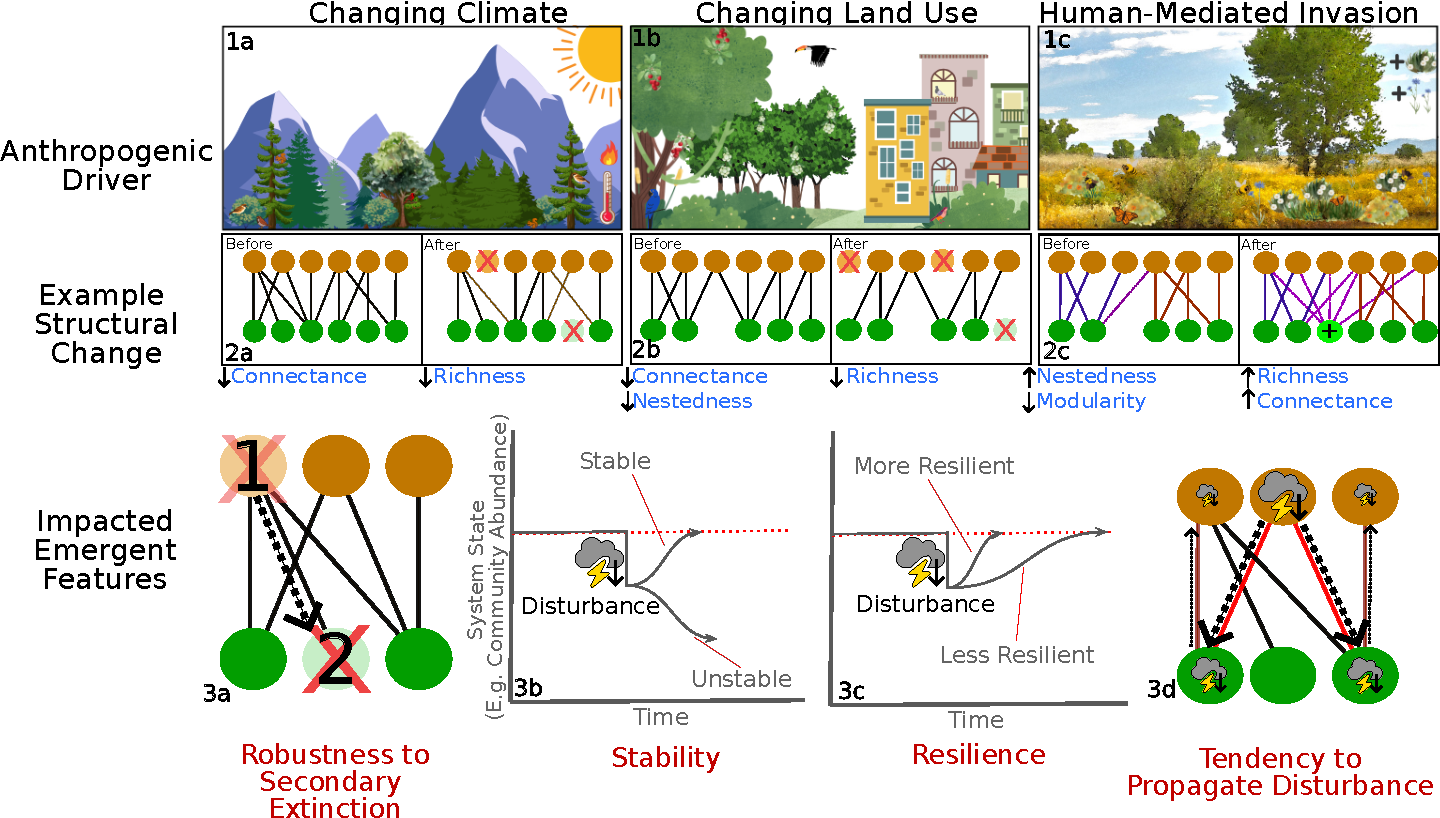
\includegraphics[width=\textwidth, alt={Graphic illustrating anthropogenic drivers of structural changes in animal-plant transport networks. The top row visualizes three main drivers, changing climate, changing land use, and human-mediated invasion, while visualizing potential network impacts. The graphic also visualized potentially impacted emergent properties of networks, including robustness to secondary extinction, stability, resilience, and tendency to propagate disturbance.}]{Review/Figures/ReviewConcept.pdf}
    \label{fig:ConceptDraft}
    \caption[Structural changes in mutualistic networks under global anthropogenic pressure]{Across a diverse set of mutualistic systems, anthropogenic drivers including changes in climate (1a), land-use patterns (1b), and the human-mediated introduction of novel mutualists (1c) can alter the structural properties of the mutualistic networks they impact (2a–2c).  These changes to component structural features may, in turn, impact emergent properties of ecological relevance (3a–3d). For example, robustness (3a) characterizes a network’s ability to avoid secondary extinctions through functional redundancy. Other emergent features describe the behavior of systems near equilibrium, including their stability—the tendency to return to equilibrium after disturbance (3b), and resilience—the speed at which they return (3c). Other features include the tendency of networks to propagate or buffer the indirect effects of disturbance (3d, where a large disturbance in the top central node's population is propagated within the network through shared links). By improving our understanding of how anthropogenic forcing elicits structural change in mutualistic networks, and how those changes translate into altered emergent properties, we can better predict and conserve mutualistic systems.}
  \end{center}
\end{figure}




                                                                  


\printbibliography %%  This is the command to use to
			       %%  insert the bibliography if you are using
                           %% the biblatex.sty package.  See the 
                           %% uscthesisdoc.pdf documentation for
                           %% for alternative bibliographic systems.     

\Appendix                 %% Use this command if you have one 
                          %% appendix. Use \Appendices if you 
\chapter{Rights to reprint work published under a CC-BY 4.0 license}
\begin{figure}[h!]
\centering
\centerline{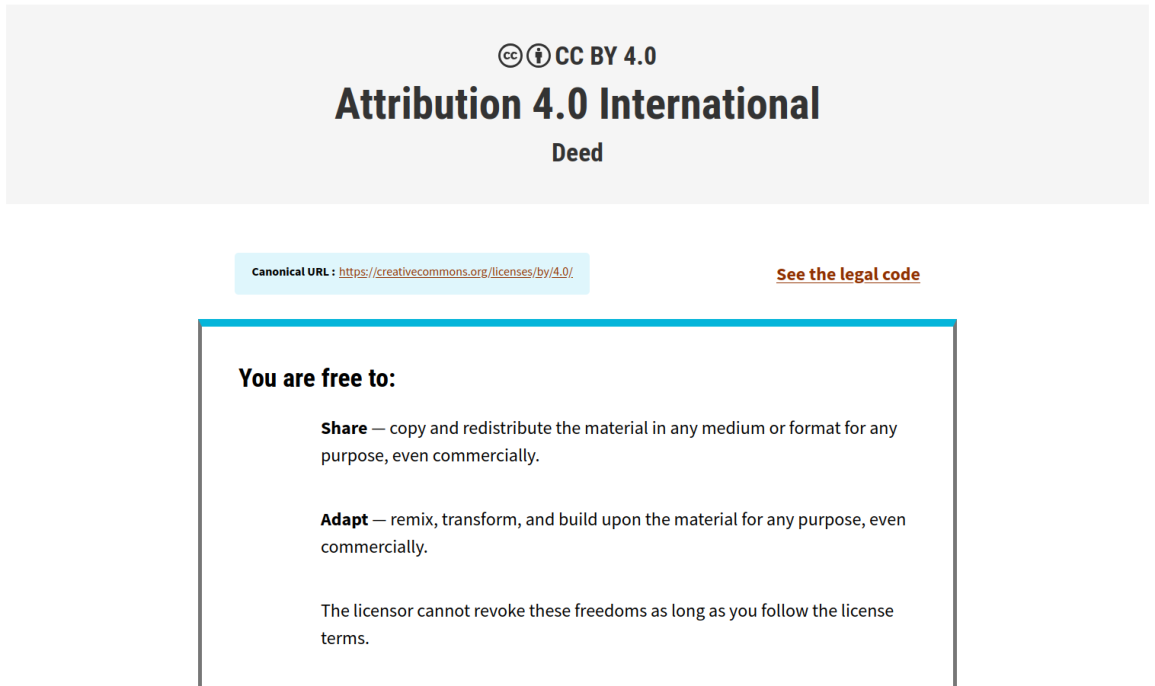
\includegraphics[width=1\textwidth]{FigCC/cc40}}
\caption[Rights to reprint open-access material]{Material that has been previously published under a CC-BY 4.0 license can be reprinted when appropriate credit is given.}
\label{fig:cc40}
\end{figure}

Chapters 2 was published under a CC-BY 4.0 license at the time of preparation of this dissertation. This license allows the reprinting of any previously published material for non-commercial use. Law regarding this license can be read here: \url{https://creativecommons.org/licenses/by/4.0/legalcode.en}
\end{document}                          %% have more than one.
\end{document}
%%%%%%%%%%%%%%%%%%%%%%%%%%%%%%%%%%%%%%%%%%%%%%%%%%%%%%%%%%%%%%%

%\printbibliography
%\setcounter{page}{103}         
\printbibliography[heading=bibintoc, title={References}] %%  This is the command to use to
			       %%  insert the bibliography if you are using			 
\addtocontents{toc}{\protect\vskip-20pt}{103}% this leads to a number showing up though in the end of refs
\addcontentsline{toc}{chapter}{References}
			       
%\addtocontents{toc}{\contentsline{section}{\numberline{9}Section Title}{15}}


%%nat bib does not work
%\bibliography{references}
%\bibliographystyle{chicago}
                           
\Appendices                 %% Use this command if you have one 
\addtocontents{toc}{\protect\vskip-20pt}
\chapter{Supplemental information for Chapter 2}
\setcounter{page}{135}         
%\section*{Methods}
\section*{\textbf{\underline{Methods}}}
\subsection*{\textbf{Random field strength}}
In the methods we explain that a random gaussian field with a random strength was added into each landscape we modelled so that each virtual species occurs in a unique species. In Figure \ref{fig:S1} we show how different levels of strength in the random field can lead to different levels of spatial autocorrelation in the environmental variable across the landscape.

\begin{figure}[h!]
\centering
%\graphicspath{ {c:/Teste/Chapter-1-Protocol/Manuscript/Plots/} }
\centerline{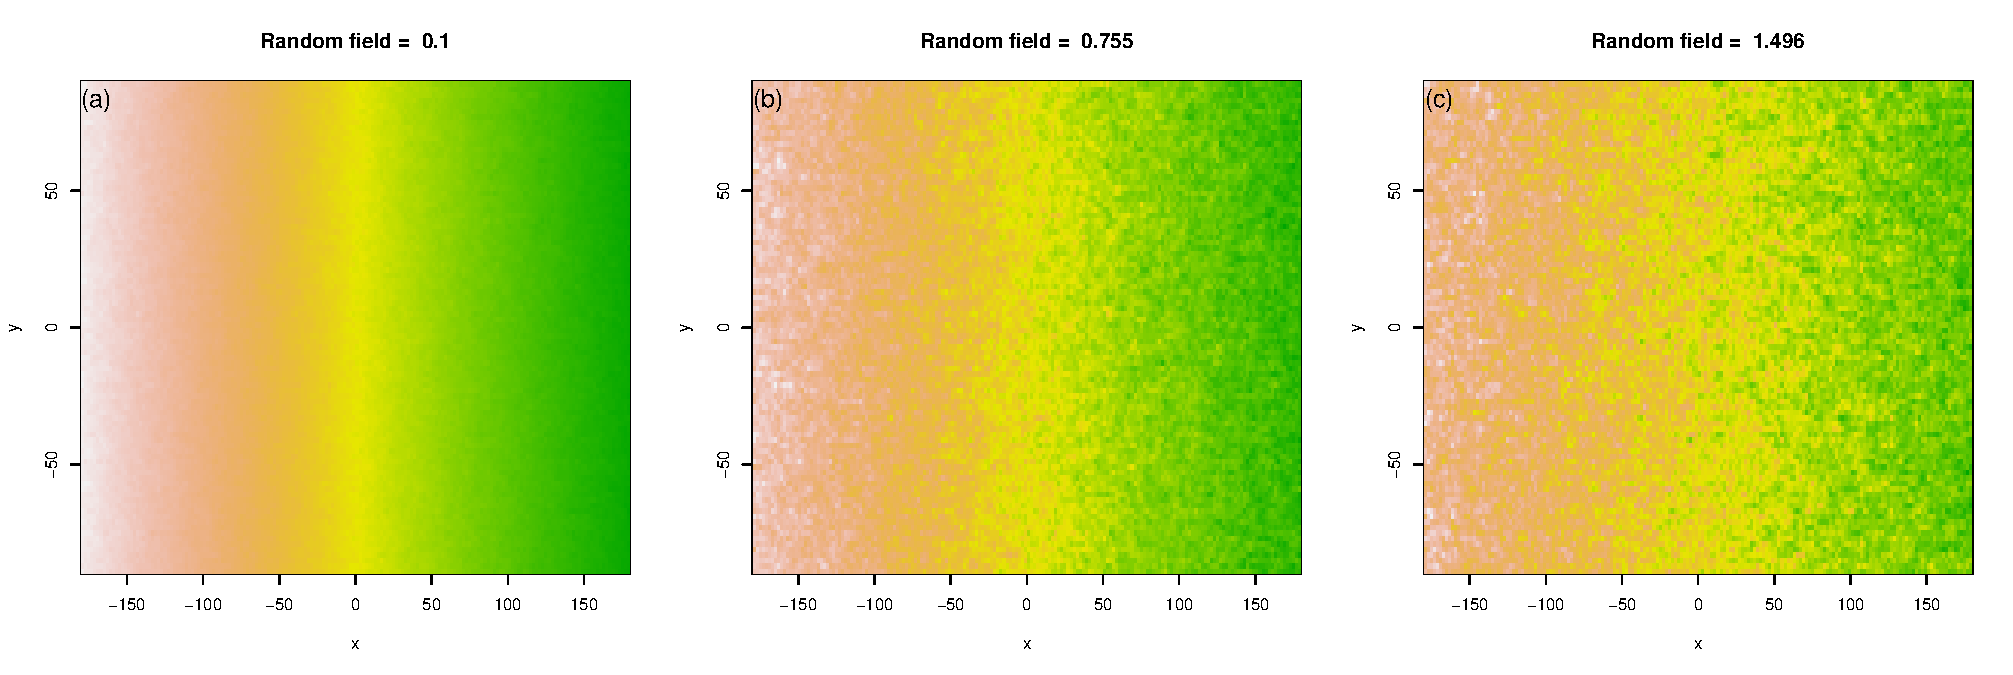
\includegraphics[width=1\textwidth]{Plots/FigureS1}}
\caption[Random fields]{Effects of the strenght of the random field on the virtual environmental gradient. As the strength of the random field increases from 0.1 (a), to 0.755 (b) and 1.49 (c) the landscape becomes less spatially autocorrelated.}
 \label{fig:S1}
\end{figure}

\subsection*{\textbf{Using unique occurrence points for model cross-validation}}
In the methods we mentioned that for the virtual species we modelled their distribution using a unique set of occurrence points for each of the 20 sampling process applied during the cross-validation of the models. To ensure that this process is comparable to the one applied to the real species (i.e., the same occurrence points were resampled 20 times), we also resampled the same set of occurrence points for 20 virtual species modelled their distribution and compared whether the performance and variation in performance of these models greatly differ from each other. In general, we found that both the model performance and variation in performance are very similar when the same and unique data are used to model the species distributions (Figure \ref{fig:S2}). This shows that the same results are obtained when both types of data are used in SDMs and that this could not have affected our study.

\begin{figure}[h!]
\centering
%\graphicspath{ {c:/Teste/Chapter-1-Protocol/Manuscript/Plots/} }
\centerline{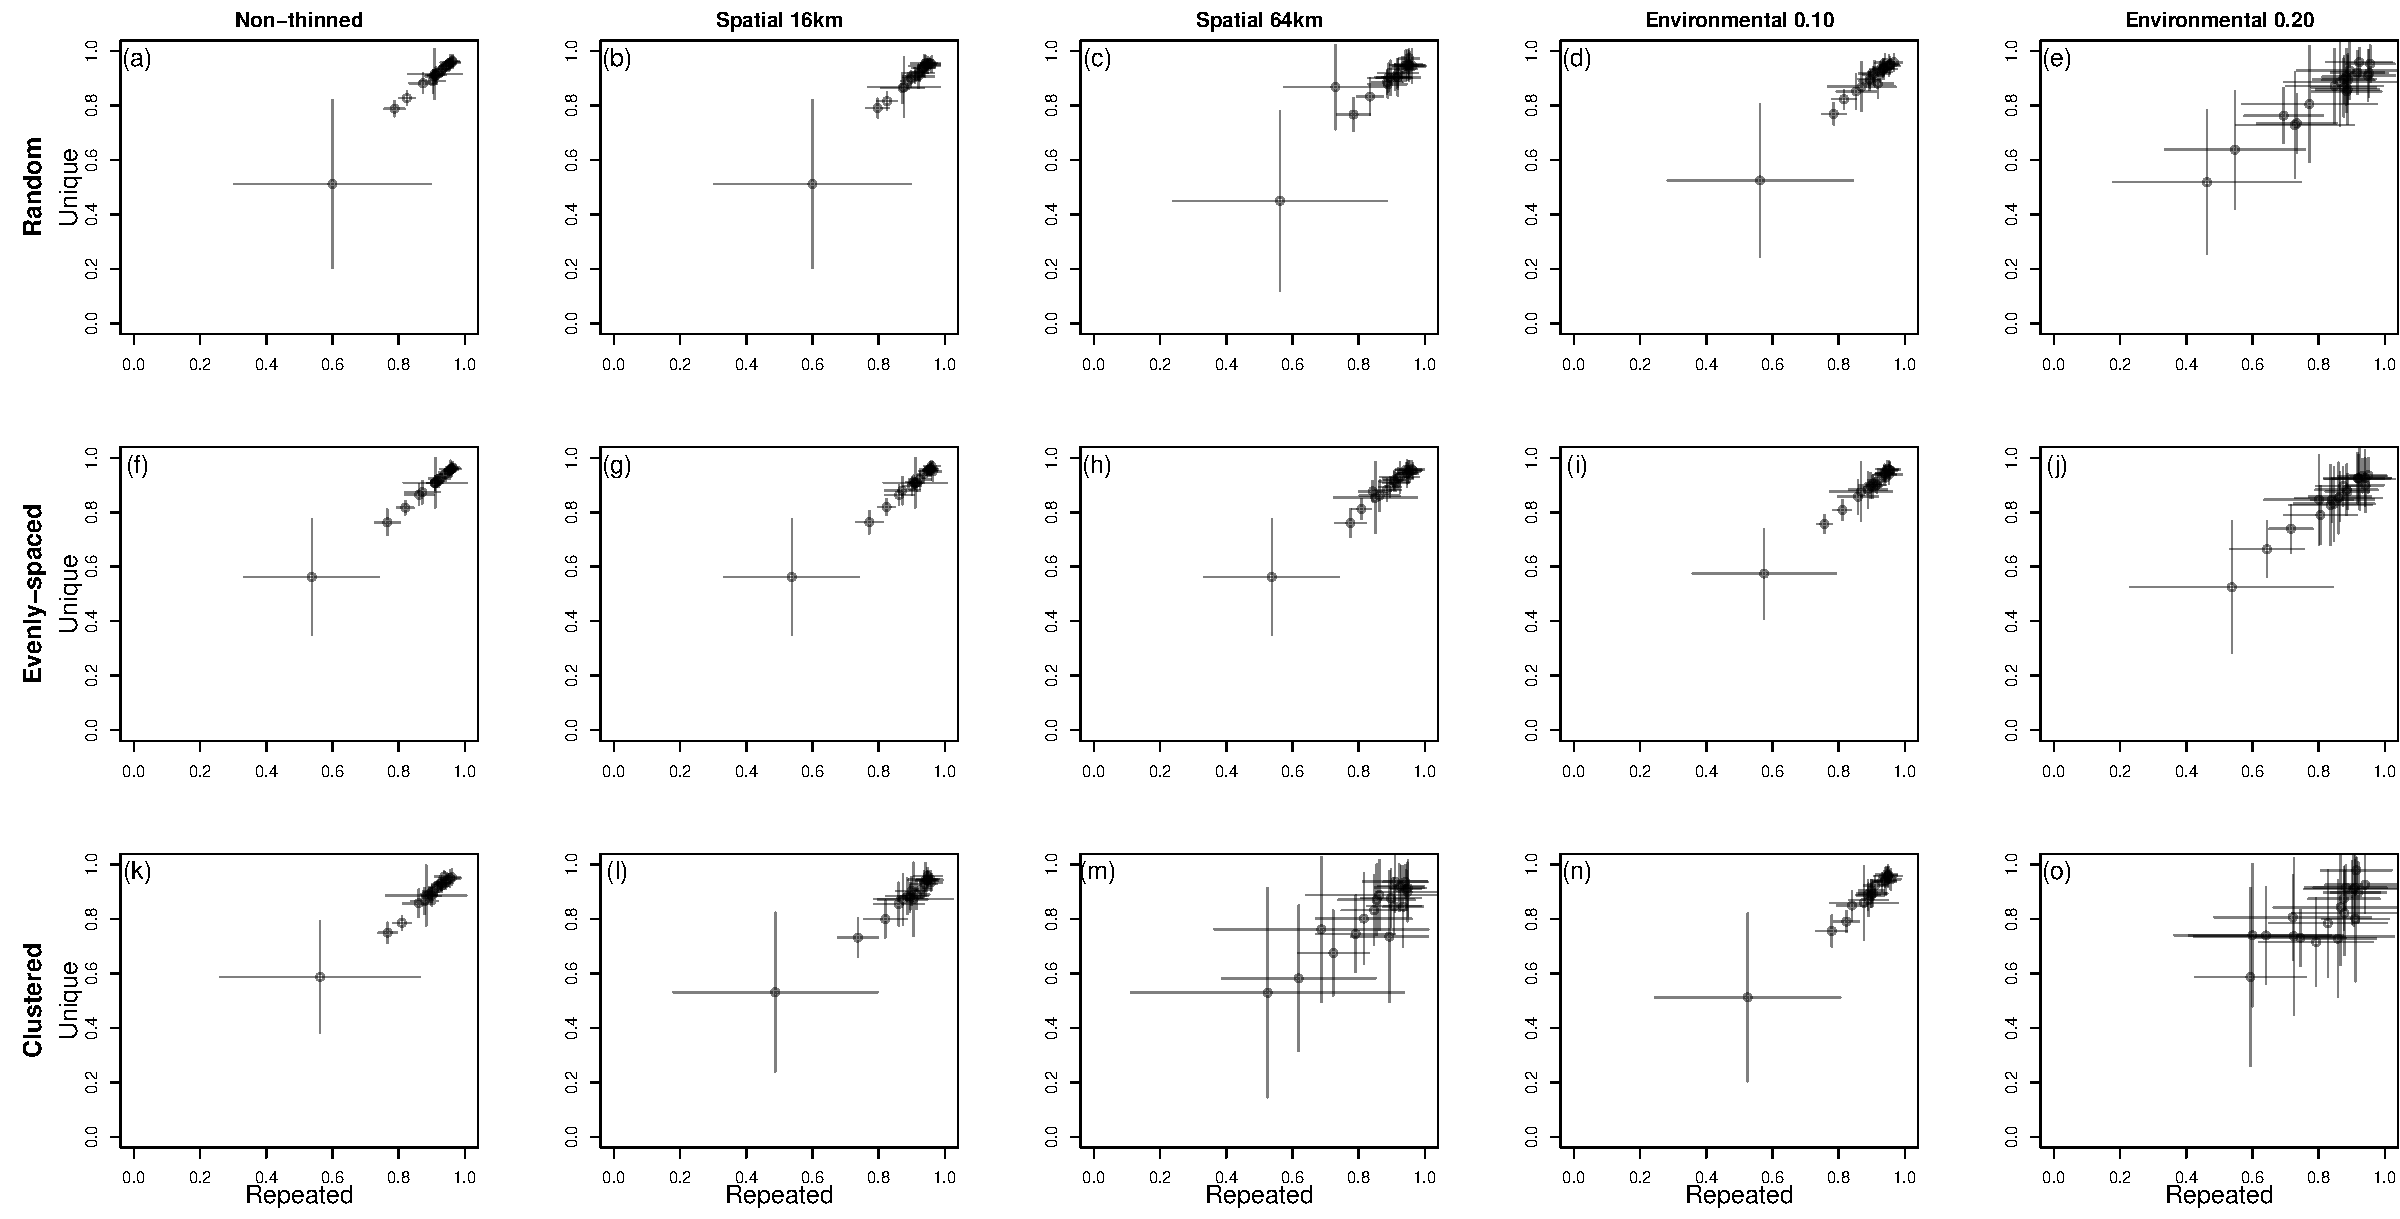
\includegraphics[width=1\textwidth]{Plots/FigureS2}}
\caption[Occurrence data type and model performance]{SDMs discrimination (AUC) when the same (x-axis) and unique (y-axis) data are used in the cross-validation sampling process for 20 virtual species with random (a-e), overdispersed (f-j), and clustered occurrence points (k-o).}
\label{fig:S2}
\end{figure}

\subsection*{\textbf{Estimating root mean square error}}
In the methods we explain that we used root mean square error to measure calibration, a for of model performance, for 10 probability bins (where they have similar sample sizes based on quantiles). We use the formula  $\sqrt{\frac{\Sigma_{i=1}^{n} (x_i - \bar {y})^2}{n}}$ to calculate RMSE for each individual bin, where $x_i$ represents the predicted occurrence probability for a specific cell within a probability bin by a model and $\bar {y}$ is the mean of a binary vector that is equivalent to the fraction of observed occurrences in that probability bin. We used $\bar {y}$ instead of $y_i$ because we only have binary (i.e., 0 and 1) data for the observed occurrences, and using them would affect the estimation of calibration. We averaged calibration across the 10 probability bins for each species considered in our study. 

The advantage of using bins to estimate calibration is that it allows for the consideration of differences in the ability of a model to perform well under different scenarios. For example, we calculated RMSE for a well (i.e., good) and a poorly (i.e., bad) calibrated model, where the predicted suitability in a bin is similar to the observed fraction of occurrences in that bin in a good model but not in the bad model. The good model had a similarly high performance across the different probability bins and, while the bad model had a general lower performance, its performance was even worse for some bins (i.e., the bins with really low or high suitability) than for others (Figure \ref{fig:rmse}). By binning the data we are able to take these differences in the performance of a model into consideration and we provide a more realistic estimation of calibration for the model. 

\begin{figure}[h!]
\centering
%\graphicspath{ {c:/Teste/Chapter-1-Protocol/Manuscript/Plots/} }
\centerline{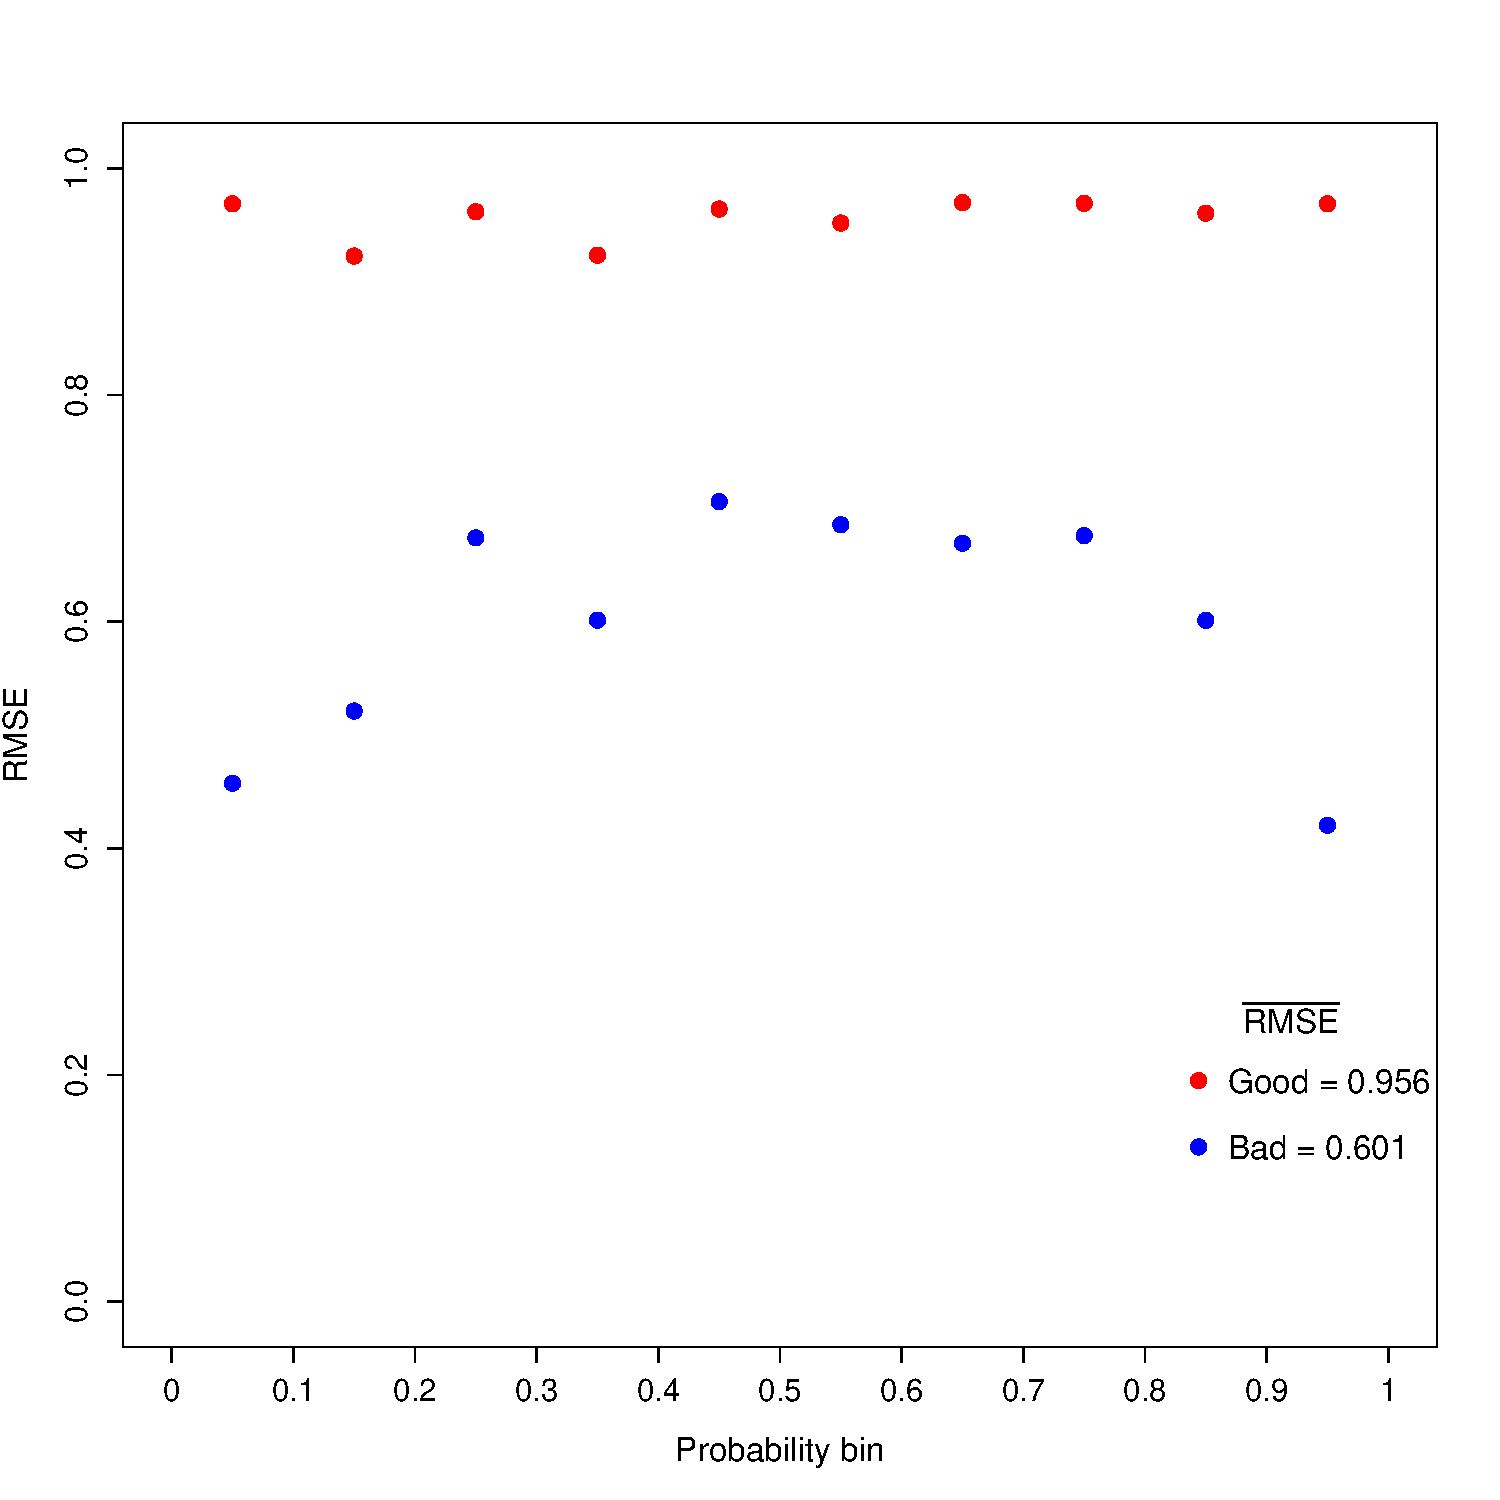
\includegraphics[width=1\textwidth]{Plots/RMSE_bins}}
\caption[Root mean square error]{Calculation of root mean square error (RMSE) for 10 probability bins (i.e., dots in the plot) considering a good and a bad model.}
 \label{fig:rmse}
\end{figure}



%\section*{Results}
\section*{\textbf{\underline{Results}}}


As expected, we found a positive relationship between thinning distance used and number of occurrence points left available for the modeling procedure, such that the amount of occurrence points available to model the species distributions rapidly decline when larger thinning distances are used.  
%\addtocontents{lof}{\protect\vskip-12pt}

\begin{figure}[h!]
\centering
%\graphicspath{ {c:/Teste/Chapter-1-Protocol/Manuscript/Plots/} }
\centerline{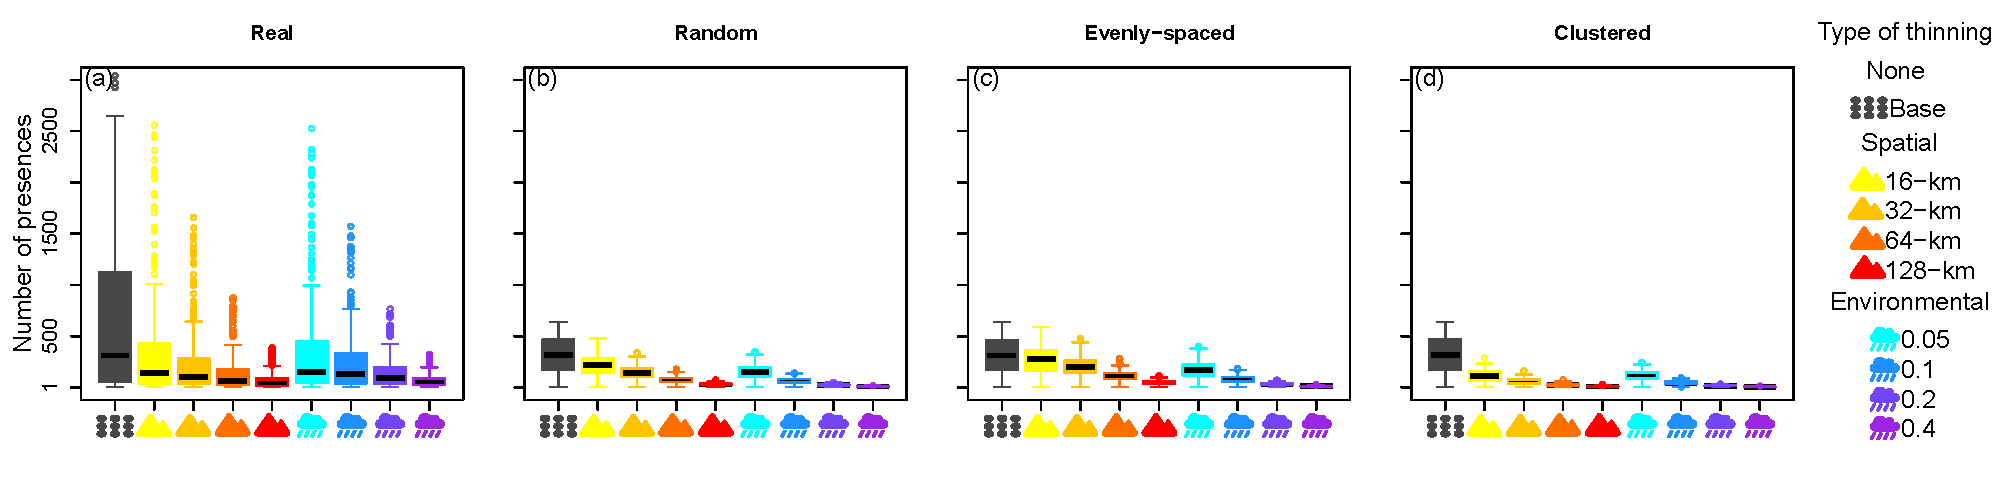
\includegraphics[width=1\textwidth]{Plots/FigureS3}}
\caption[Number of occurrence points]{Number of occurrence points available for the modeling of the real (a), and virtual species with random (b), clustered (c) and evenly-spaced (d) bias}
\label{fig:S3}
\end{figure}

In the results section of the main text we mainly report the effects of thinning occurrence points on the discrimination power of MaxEnt while the effects of thinning on SVM, GLM, and GAM were only briefly mentioned. Here, we describe in details the effects of thinning on the different performance metrics of these modeling methods. 

\subsection*{\textbf{Using MaxEnt}}
%\addtocontents{lof}{\protect\vskip-12pt}

Spatial and environmental thinning decreased MaxEnt accuracy and calibration in a similar manner for real (Figure \ref{fig:S4}a, Figure \ref{fig:S6}a) and virtual (Figure \ref{fig:S4}b-d, Figure \ref{fig:S6}b-d) species. In these cases, spatial thinning had stronger negative effects on MaxEnt accuracy and calibration of real species and virtual species with clustered occurrence points whereas virtual species with random and evenly-spaced occurrence points were more negatively affected by environmental thinning. Nevertheless, the negative effects of environmental thinning on MaxEnt accuracy and calibration were significant and consistent across real and virtual species. Similarly, spatial and environmental thinning also decreased MaxEnt precision of virtual (Figure \ref{fig:S5}b-d) species, where all the species were similarly affected by the thinning approaches, and to a lower degree for real (Figure \ref{fig:S5}a) species. In general, the negative effects of thinning were similar across the different types of spatial biases and tended to be stronger when larger thinning distances were used.

%\addtocontents{lof}{\protect\vskip-12pt}

\begin{figure}[h!]
\centering
%\graphicspath{ {c:/Teste/Chapter-1-Protocol/Manuscript/Plots/} }
\centerline{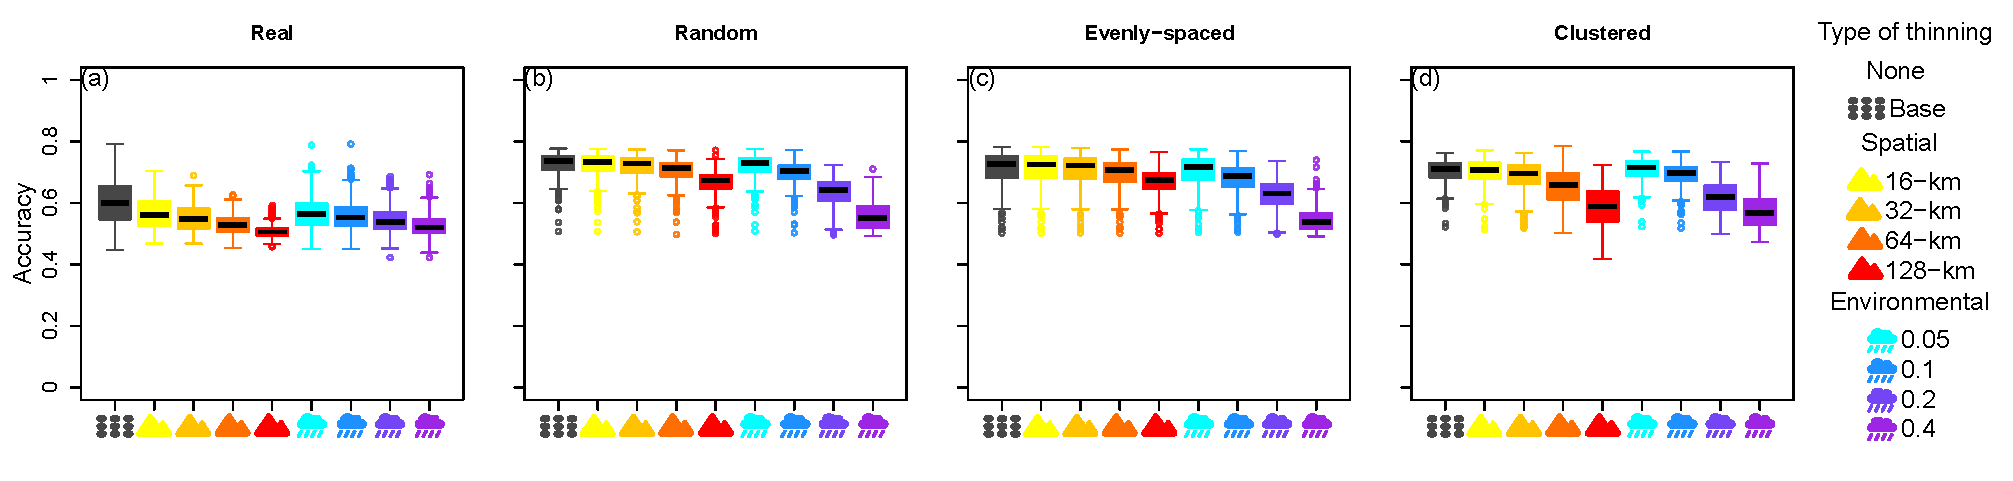
\includegraphics[width=1\textwidth]{Plots/FigureS4}}
\caption[Effects of thinning on MaxEnt accuracy]{The effects of spatial and environmental thinning on MaxEnt accuracy of real species (a), and virtual species with random (b), clustered (c), and evenly-spaced (d) sampled occurrence points.}
 \label{fig:S4}
\end{figure}

%\addtocontents{lof}{\protect\vskip-12pt}

\begin{figure}[h!]
\centering
%\graphicspath{ {c:/Teste/Chapter-1-Protocol/Manuscript/Plots/} }
\centerline{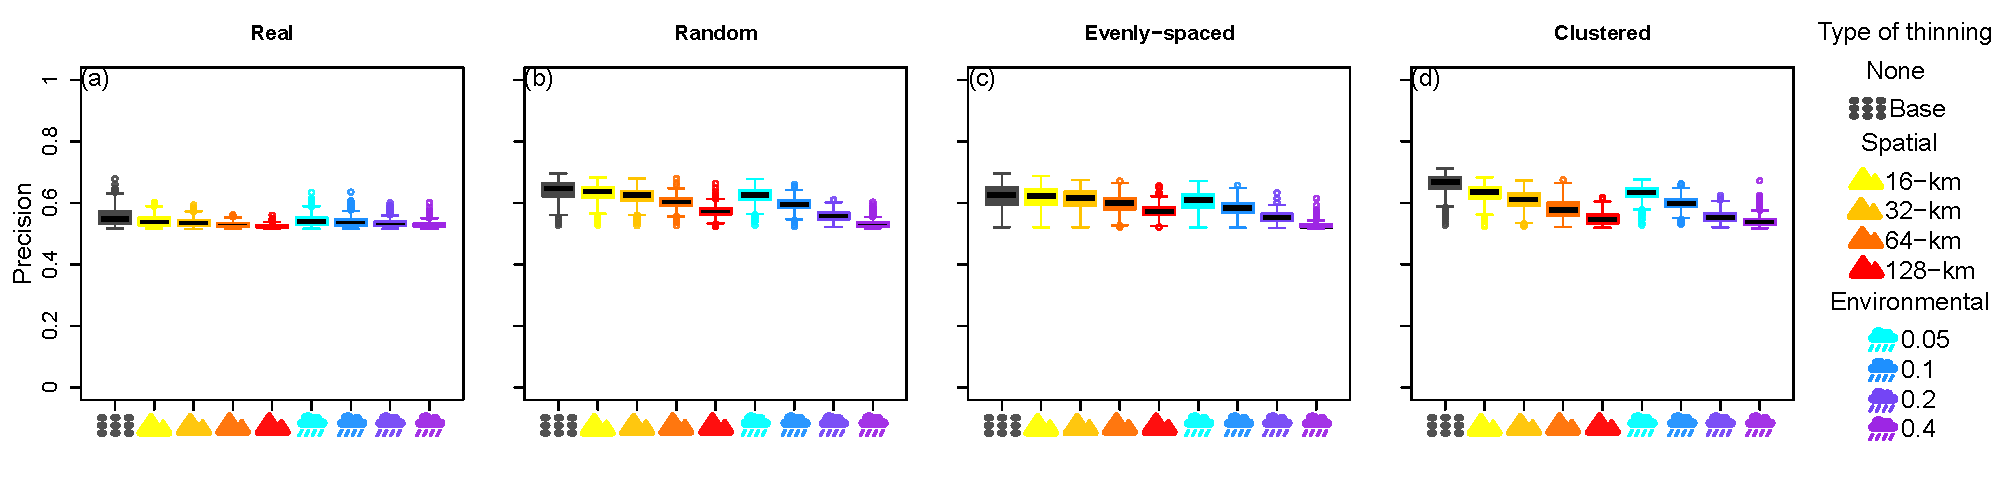
\includegraphics[width=1\textwidth]{Plots/FigureS5}} 
\caption[Effects of thinning on MaxEnt precision]{The effects of spatial and environmental thinning on MaxEnt precision of real species (a), and virtual species with random (b), clustered (c), and evenly-spaced (d) sampled occurrence points.}
 \label{fig:S5}
\end{figure}

%\addtocontents{lof}{\protect\vskip-12pt}

\begin{figure}[h!]
\centering
%\graphicspath{ {c:/Teste/Chapter-1-Protocol/Manuscript/Plots/} }
\centerline{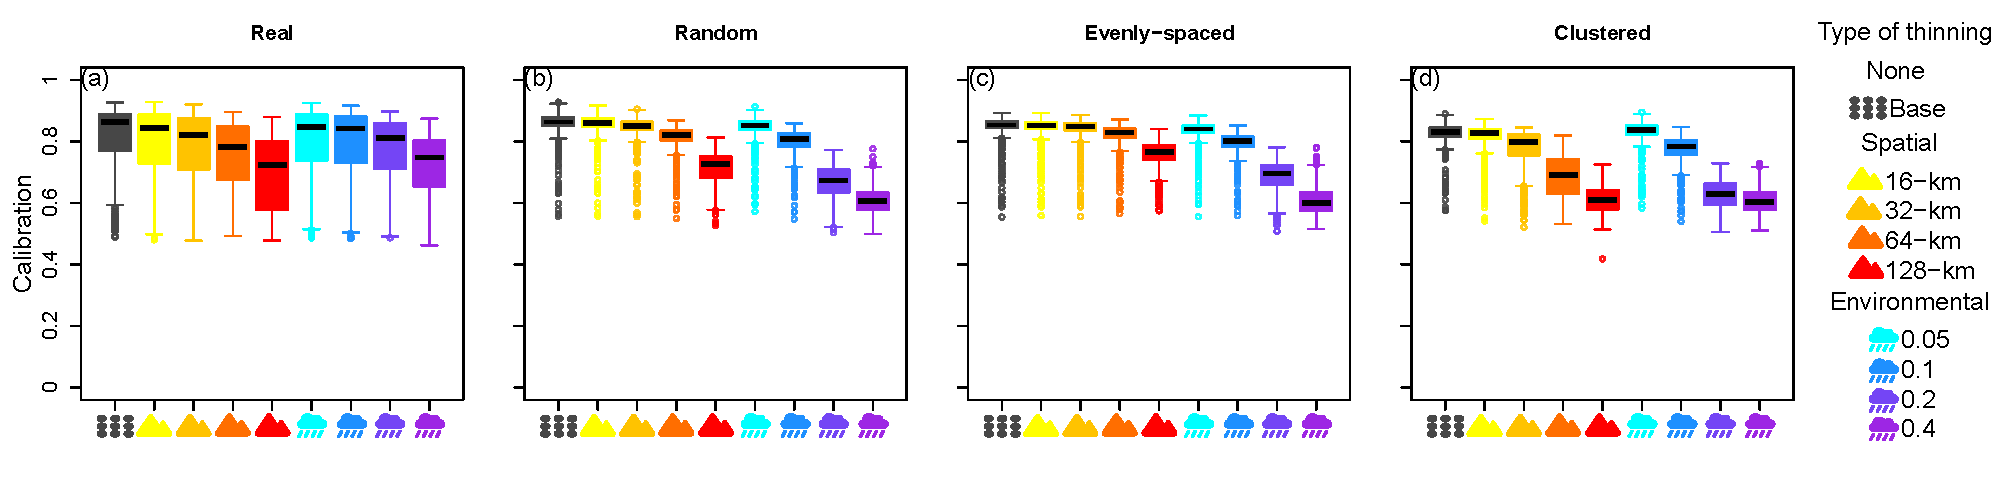
\includegraphics[width=1\textwidth]{Plots/FigureS6}}
\caption[Effects of thinning on MaxEnt calibration]{The effects of spatial and environmental thinning on MaxEnt calibration of real species (a), and virtual species with random (b), clustered (c), and evenly-spaced (d) sampled occurrence points.}
 \label{fig:S6}
\end{figure}

\subsection*{\textbf{Using SVM}}
In general, SVM was less susceptible to the negative effects of thinning occurrence points than GAM and MaxEnt. Spatial and environmental thinning similarly decreased SVM discrimination for real species (Figure \ref{fig:S7}a). On the other hand, only when the largest thinning distances were used did environmental thinning decrease discrimination for virtual species (Figure \ref{fig:S7}b-d). Spatial and environmental thinning decreased SVM accuracy and calibration similarly for real (Figure \ref{fig:S8}a, Figure \ref{fig:S10}a) and virtual species (Figure \ref{fig:S8}b-d, Figure \ref{fig:S10}b-d), where spatial thinning had stronger negative effects on real species and virtual species with clustered occurrences and environmental thinning had stronger negative effects on virtual species with random and evenly-dispersed occurrences. On the other hand, spatial and environmental thinning had only a slight negative effect on SVM precision for real (Figure \ref{fig:S9}a) and virtual (Figure \ref{fig:S9}b-d) species that was observed mostly when the largest thinning distances were used. Thus, although to a lower degree, we still observed a consistent negative effect of thinning on SVM performance across the different types of spatial bias we considered, and these negative effects tended to be stronger the larger the thinning distance used. 




%SVM was the modelling method that was the most resistent to thinning, but the negative impacts were still noticeable especially when larger thinnning distances were used.
\begin{figure}[h!]
\centering
%\graphicspath{ {c:/Teste/Chapter-1-Protocol/Manuscript/Plots/} }
\centerline{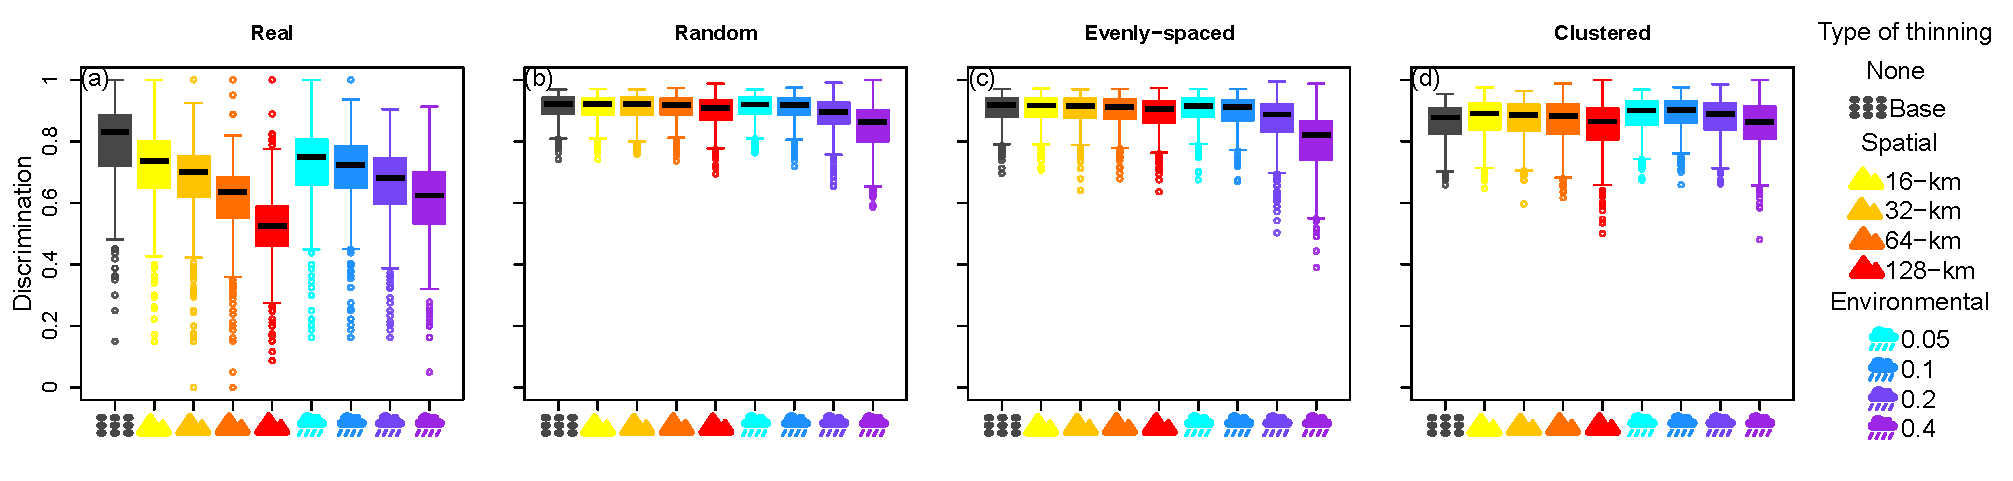
\includegraphics[width=1\textwidth]{Plots/FigureS7}}
\caption[Effects of thinning on SVM discrimination]{The effects of spatial and environmental thinning on SVM discrimination (AUC) of real species (a), and virtual species with random (b), clustered (c), and evenly-spaced (d) sampled occurrence points.}
 \label{fig:S7}
\end{figure}


\begin{figure}[h!]
\centering
%\graphicspath{ {c:/Teste/Chapter-1-Protocol/Manuscript/Plots/}  }
\centerline{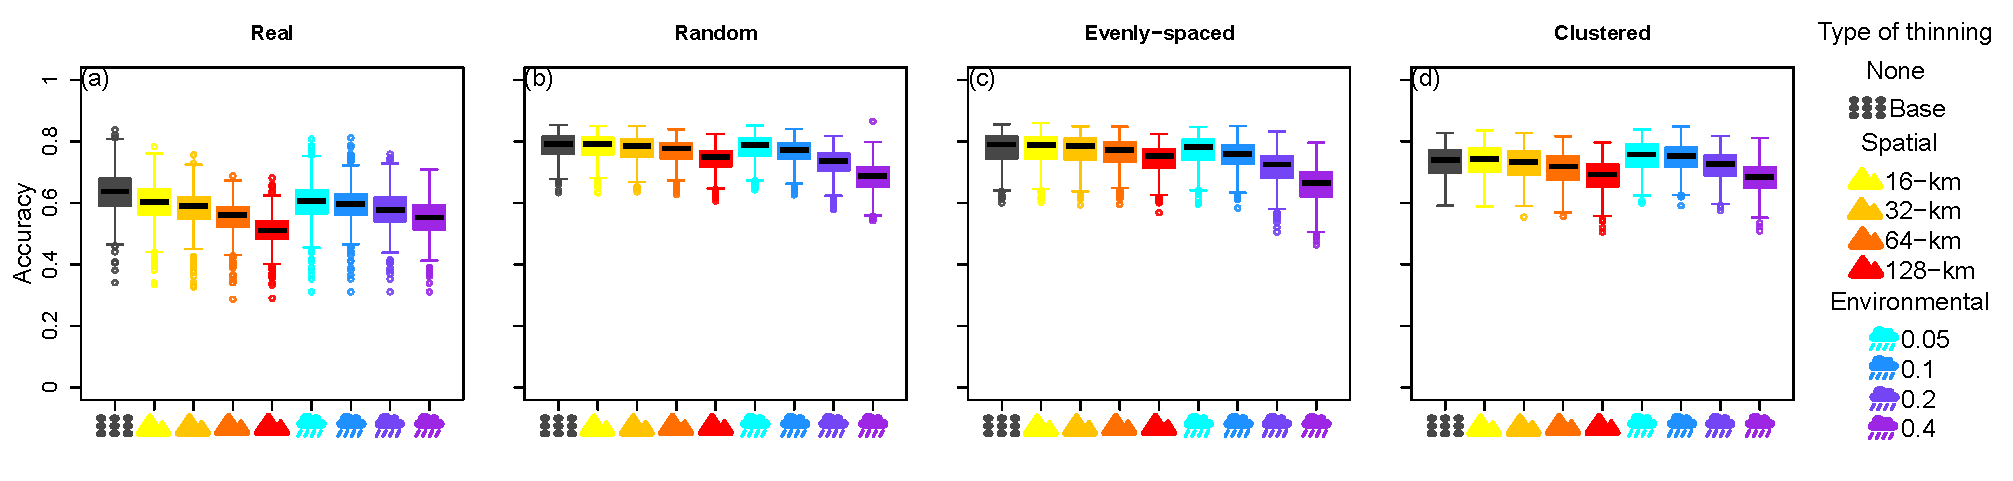
\includegraphics[width=1\textwidth]{Plots/FigureS8}} 
\caption[Effects of thinning on SVM accuracy]{The effects of spatial and environmental thinning on SVM accuracy of real species (a), and virtual species with random (b), clustered (c), and evenly-spaced (d) sampled occurrence points.}
 \label{fig:S8}
\end{figure}

\begin{figure}[h!]
\centering
%\graphicspath{ {c:/Teste/Chapter-1-Protocol/Manuscript/Plots/} }
\centerline{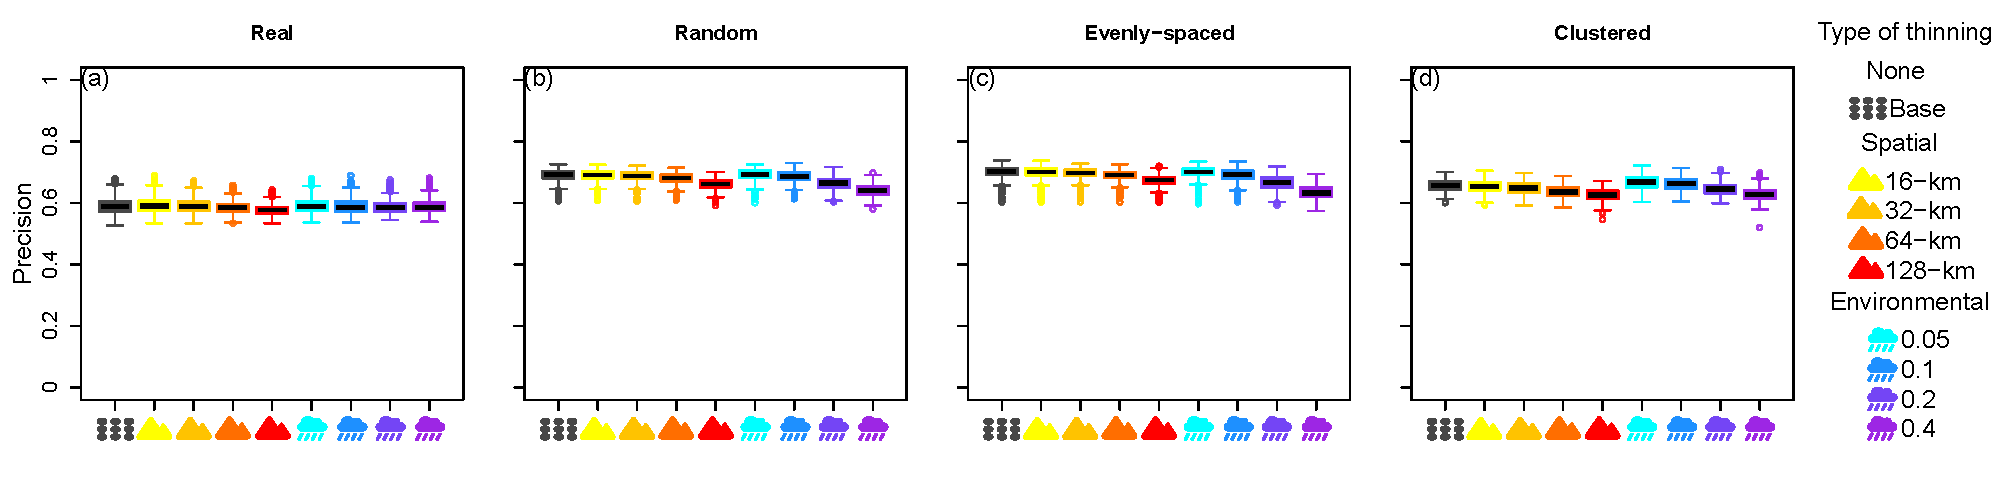
\includegraphics[width=1\textwidth]{Plots/FigureS9}} 
\caption[Effects of thinning on SVM precision]{The effects of spatial and environmental thinning on SVM precision of real species (a), and virtual species with random (b), clustered (c), and evenly-spaced (d) sampled occurrence points.}
 \label{fig:S9}
\end{figure}

\begin{figure}[h!]
\centering
%\graphicspath{ {c:/Teste/Chapter-1-Protocol/Manuscript/Plots/}  }
\centerline{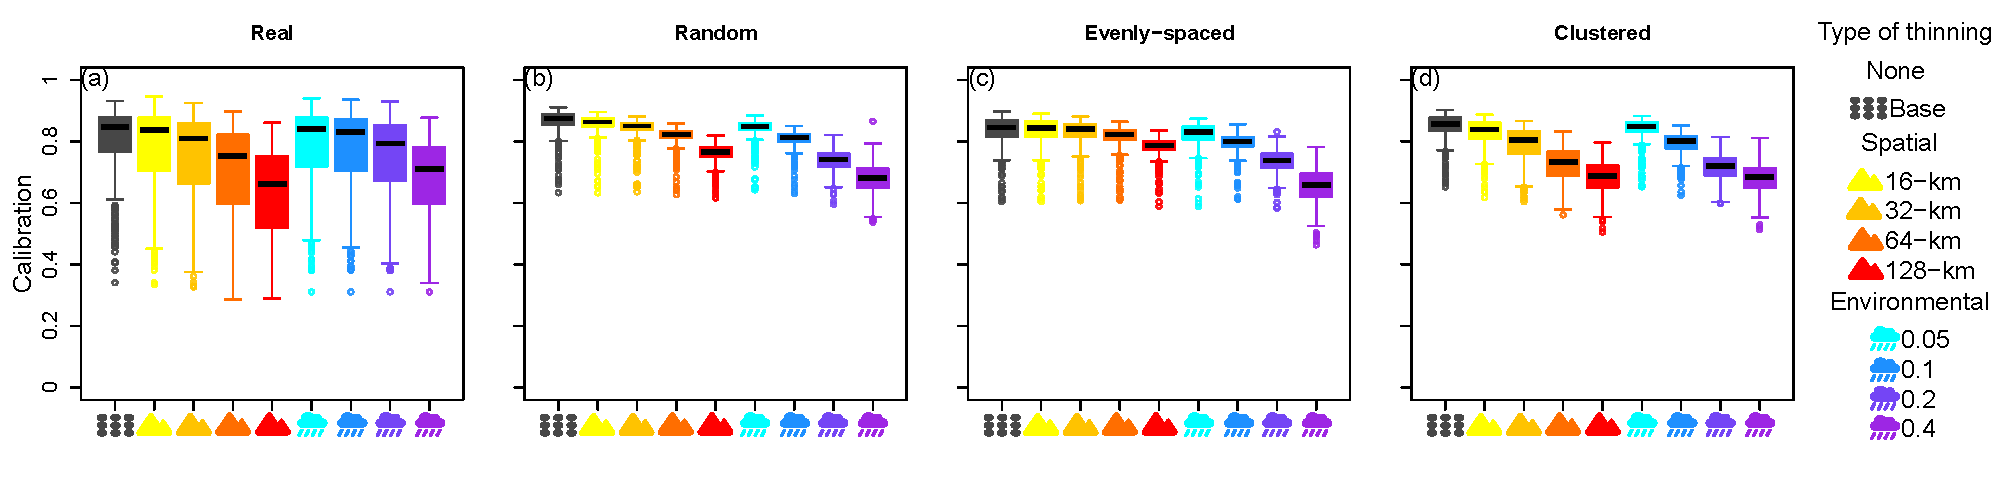
\includegraphics[width=1\textwidth]{Plots/FigureS10}} 
\caption[Effects of thinning on SVM calibration]{The effects of spatial and environmental thinning on SVM calibration of real species (a), and virtual species with random (b), clustered (c), and evenly-spaced (d) sampled occurrence points.}
 \label{fig:S10}
\end{figure}



\subsection*{\textbf{Using GLM}}
Similarly to SVM, thinning also affected GLM performance to a smaller extent. Spatial and environmental thinning decreased discrimination of GLM for real (Figure \ref{fig:S11}a) and virtual (Figure \ref{fig:S11}b-d) species, although the negative thinning effects on virtual species were much smaller and only noticeable when the largest thinning distances were used. While spatial and environmental thinning decreased GLM accuracy for real species (Figure \ref{fig:S12}a), virtual species remained largely unaffected by thinning (Figure \ref{fig:S12}b-d). Moreover, spatial and environmental thinning did not affect GLM precision for real species (Figure \ref{fig:S13}a) and virtual species with random and evenly-spaced occurrences (Figure \ref{fig:S13}b-c), but the use of larger spatial and environmental thinning distances led to an increase in precision for virtual species with clustered occurrences (Figure \ref{fig:S13}d). On the other hand, spatial and environmental thinning decreased GLM calibration for real (Figure \ref{fig:S14}a) and virttual species (Figure \ref{fig:S14}b-d), where spatial thinning had a stronger negative impact on real species and virtual species with clustered occurrences and environmental thinning had stronger negative effects on virtual species with random and evenly-spaced occurrences. In general, the negative effects of thinning on GLM tended to stronger the larger the thinning distance used. Thus, even though thinning positively affected GLM precision for species with clustered occurrences, this has little significance given that the general effects of thinning were negative or neutral for all other circumstances and that GLM had the worst general performance among all modeling methods we considered. 

\begin{figure}[h!]
\centering
%\graphicspath{ {c:/Teste/Chapter-1-Protocol/Manuscript/Plots/}  }
\centerline{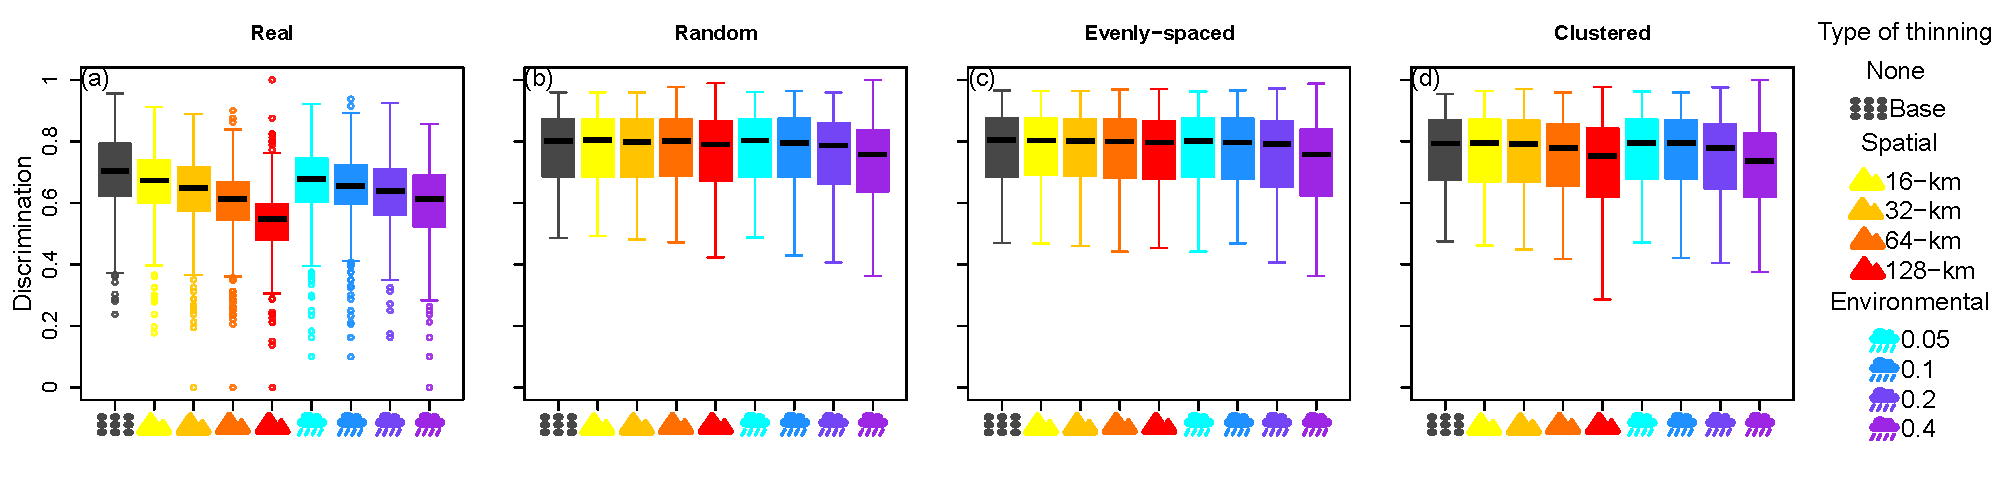
\includegraphics[width=1\textwidth]{Plots/FigureS11}} 
\caption[Effects of thinning on GLM discrimination]{The effects of spatial and environmental thinning on GLM discrimination (AUC) of real species (a), and virtual species with random (b), clustered (c), and evenly-spaced (d) sampled occurrence points.}
 \label{fig:S11}
\end{figure}
\clearpage
\begin{figure}[h!]
\centering
%\graphicspath{ {c:/Teste/Chapter-1-Protocol/Manuscript/Plots/}  }
\centerline{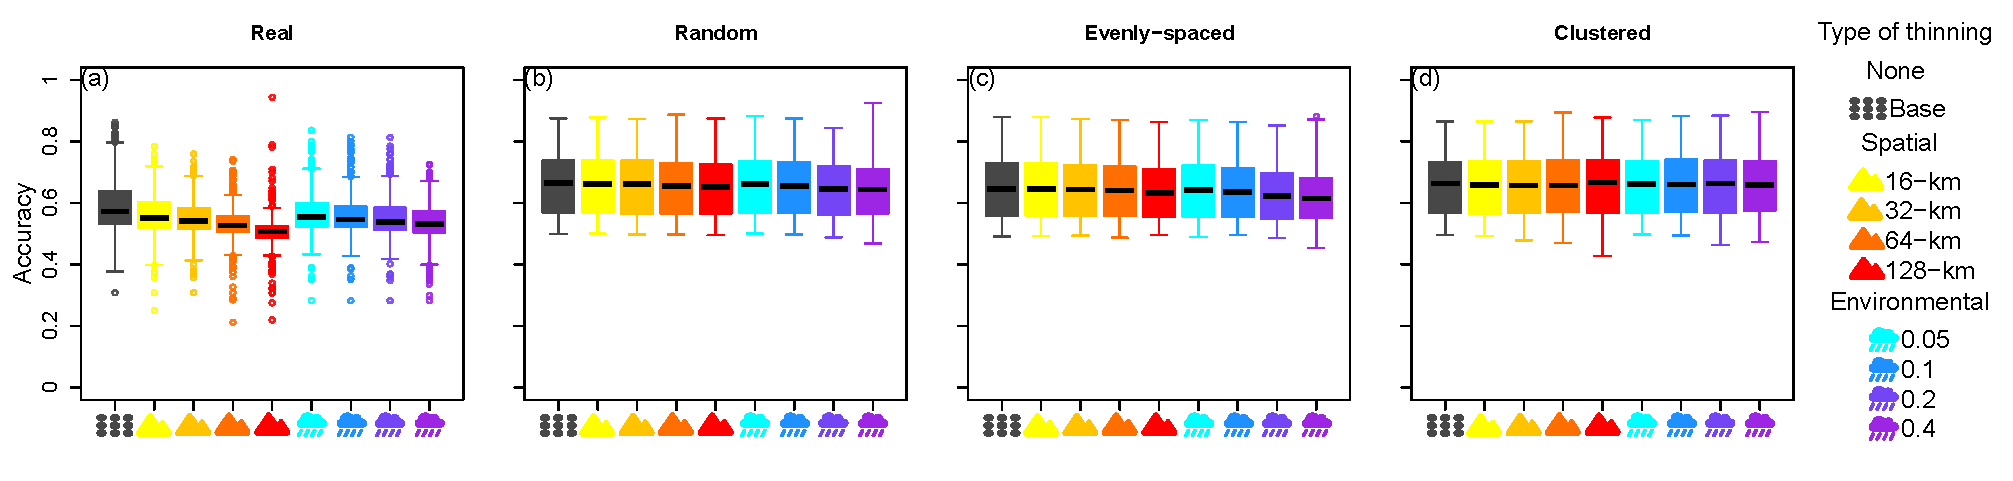
\includegraphics[width=1\textwidth]{Plots/FigureS12}} 
\caption[Effects of thinning on GLM accuracy]{The effects of spatial and environmental thinning on GLM accuracy of real species (a), and virtual species with random (b), clustered (c), and evenly-spaced (d) sampled occurrence points.}
 \label{fig:S12}
\end{figure}

\begin{figure}[h!]
\centering
%\graphicspath{ {c:/Teste/Chapter-1-Protocol/Manuscript/Plots/}  }
\centerline{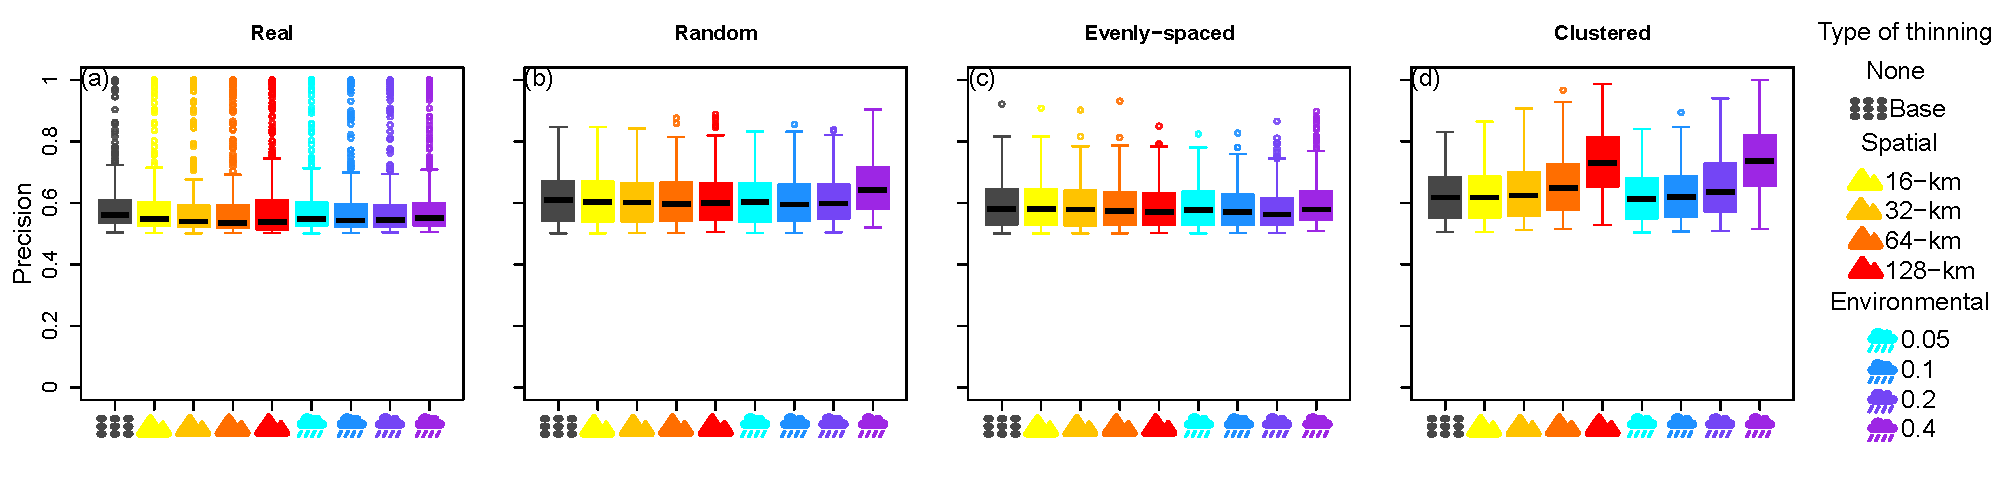
\includegraphics[width=1\textwidth]{Plots/FigureS13}} 
\caption[Effects of thinning on GLM precision]{The effects of spatial and environmental thinning on GLM precision of real species (a), and virtual species with random (b), clustered (c), and evenly-spaced (d) sampled occurrence points.}
 \label{fig:S13}
\end{figure}

\begin{figure}[h!]
\centering
%\graphicspath{ {c:/Teste/Chapter-1-Protocol/Manuscript/Plots/}  }
\centerline{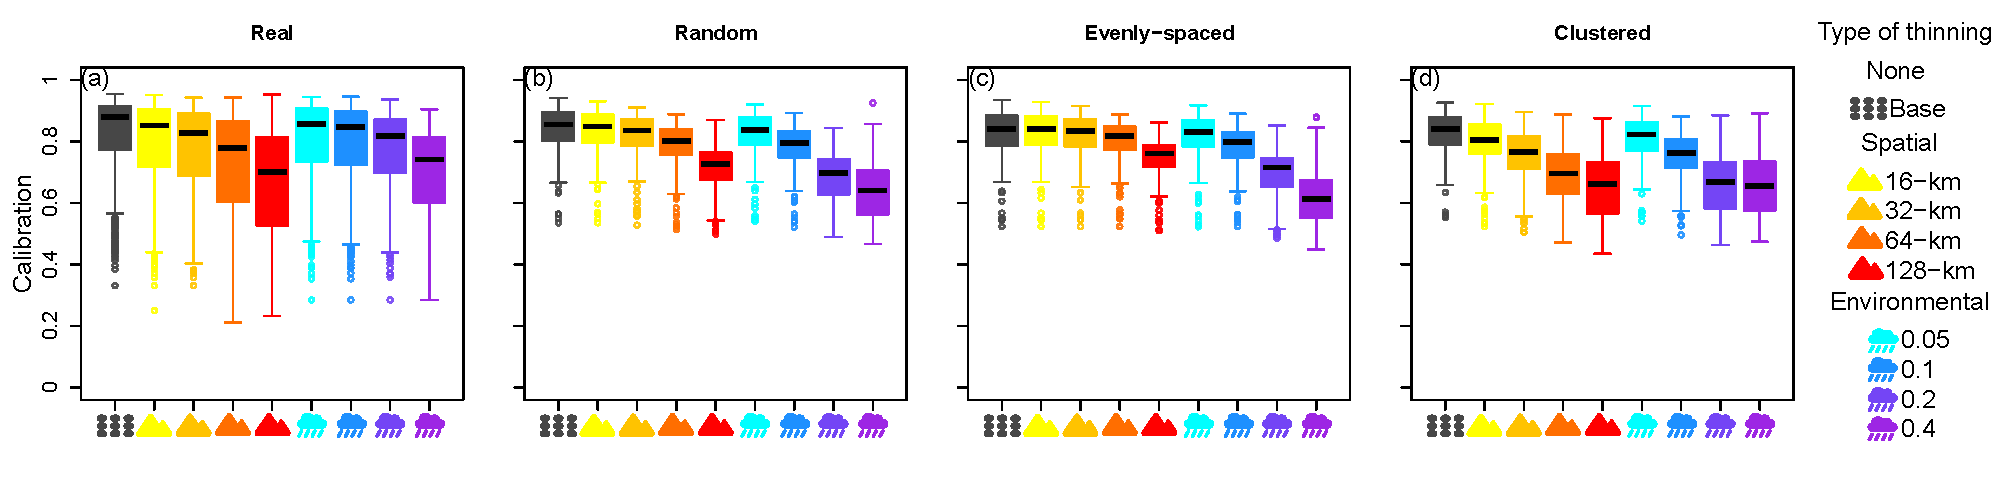
\includegraphics[width=1\textwidth]{Plots/FigureS14}} 
\caption[Effects of thinning on GLM calibration]{The effects of spatial and environmental thinning on GLM calibration of real species (a), and virtual species with random (b), clustered (c), and evenly-spaced (d) sampled occurrence points.}
 \label{fig:S14}
\end{figure}
 
\subsection*{\textbf{Using GAM}}

Thinning occurrence points affected GAM performance similarly to MaxEnt. Spatial and environmental thinning smilarly decreased discrimination, accuracy and calibration of GAM for real species (Figure \ref{fig:S15}a, \ref{fig:S16}a, \ref{fig:S18}a) and virtual (Figure \ref{fig:S15}b-d, \ref{fig:S16}b-d, \ref{fig:S18}b-d) species. In these cases, environmental thinning had a stronger negative effect on GAM discrimination, accuracy and calibration of virtual species with random and evenly-spaced occurrence points whereas both environmental and spatial thinning had equally strong negative effects on GAM discrimination, accuracy and calibration of virtual species with clustered occurrence points. In contrast, spatial and environmental thinning increased GAM precision for real (Figure \ref{fig:S17}a) and virtual (Figure \ref{fig:S17}b-d) species especially when larger thinning distances were used, although this result has no significance given that model accuracy decreased when thinning was used. Overall, our results show that spatial and environmental thinning had consistent negative effects on GAM performance, and that these negative effects tended to be stronger when larger thinning distances were used.




\begin{figure}[h!]
\centering
%\graphicspath{ {c:/Teste/Chapter-1-Protocol/Manuscript/Plots/}  }
\centerline{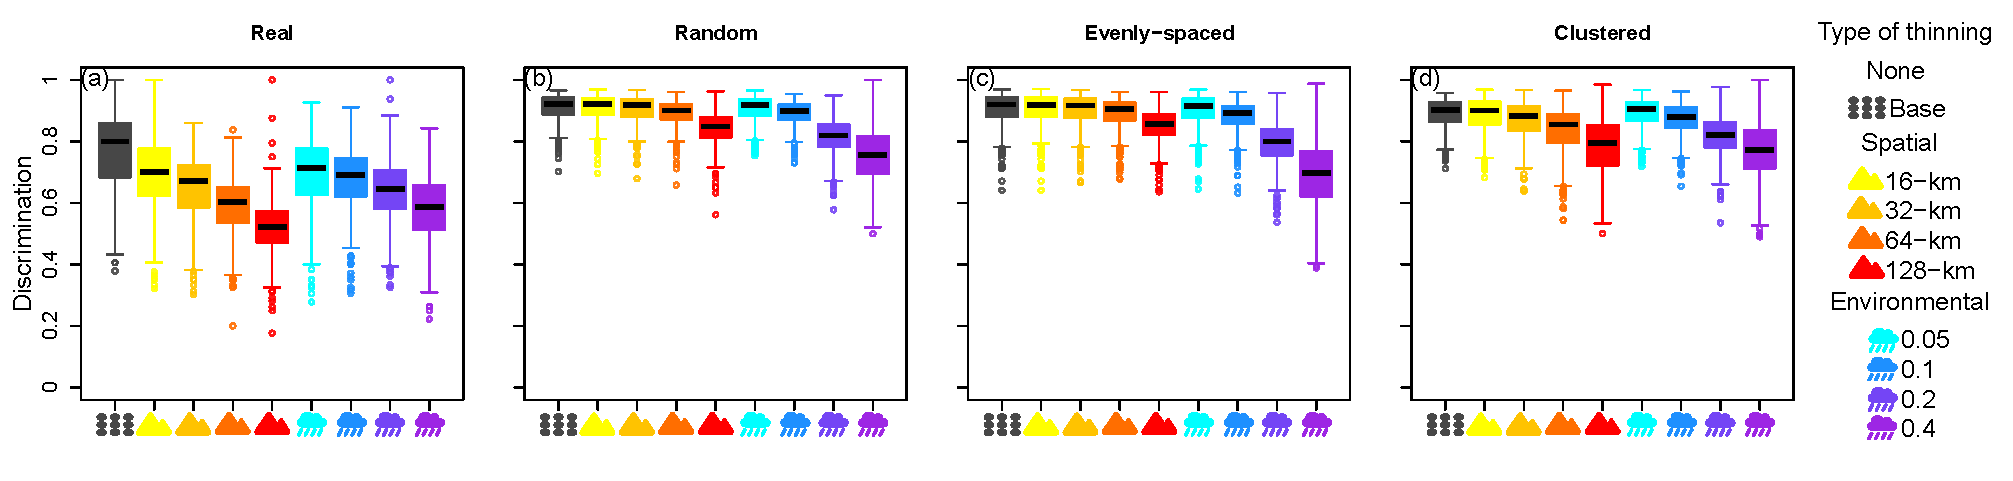
\includegraphics[width=1\textwidth]{Plots/FigureS15}} 
\caption[Effects of thinning on GAM discrimination]{The effects of spatial and environmental thinning on GAM discrimination (AUC) of real species (a), and virtual species with random (b), clustered (c), and evenly-spaced (d) sampled occurrence points.}
 \label{fig:S15}
\end{figure}

\begin{figure}[h!]
\centering
%\graphicspath{ {c:/Teste/Chapter-1-Protocol/Manuscript/Plots/}  }
\centerline{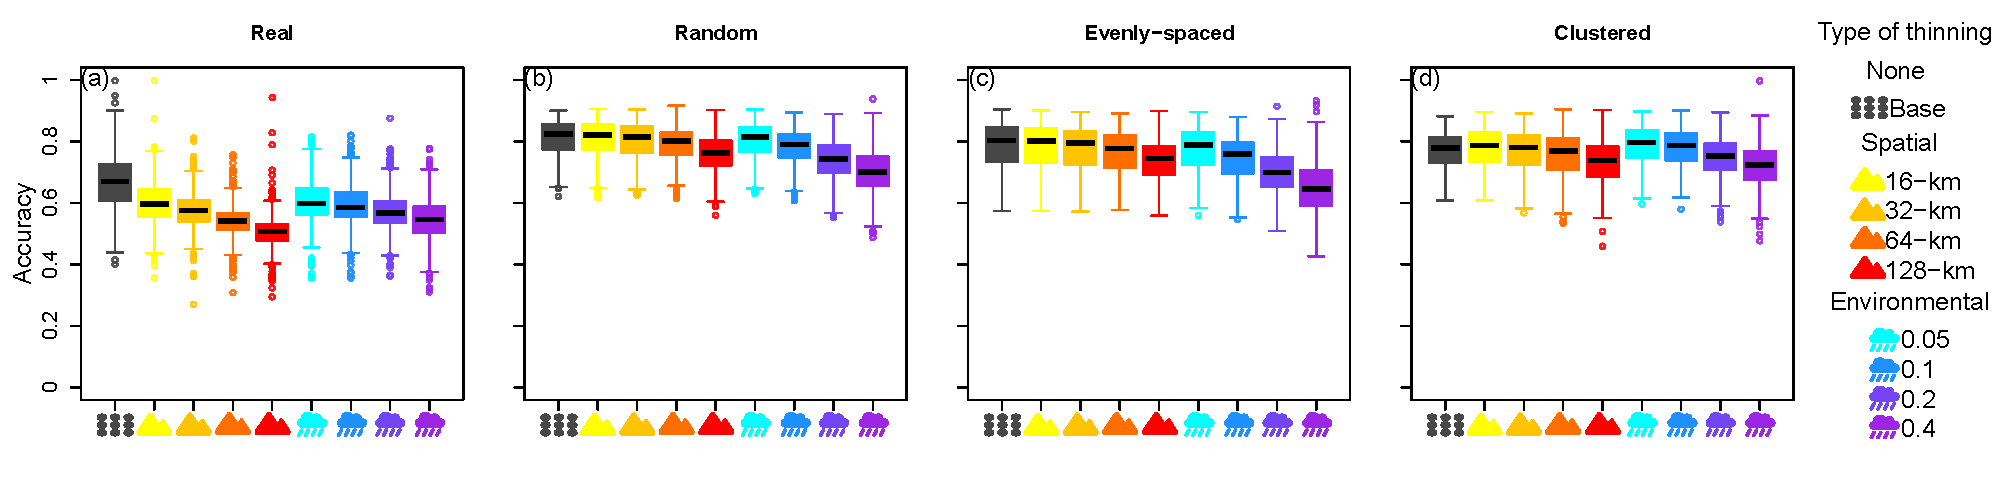
\includegraphics[width=1\textwidth]{Plots/FigureS16}} 
\caption[Effects of thinning on GAM accuracy]{The effects of spatial and environmental thinning on GAM accuracy of real species (a), and virtual species with random (b), clustered (c), and evenly-spaced (d) sampled occurrence points.}
 \label{fig:S16}
\end{figure}

\clearpage
\begin{figure}[h!]
\centering
%\graphicspath{ {c:/Teste/Chapter-1-Protocol/Manuscript/Plots/}  }
\centerline{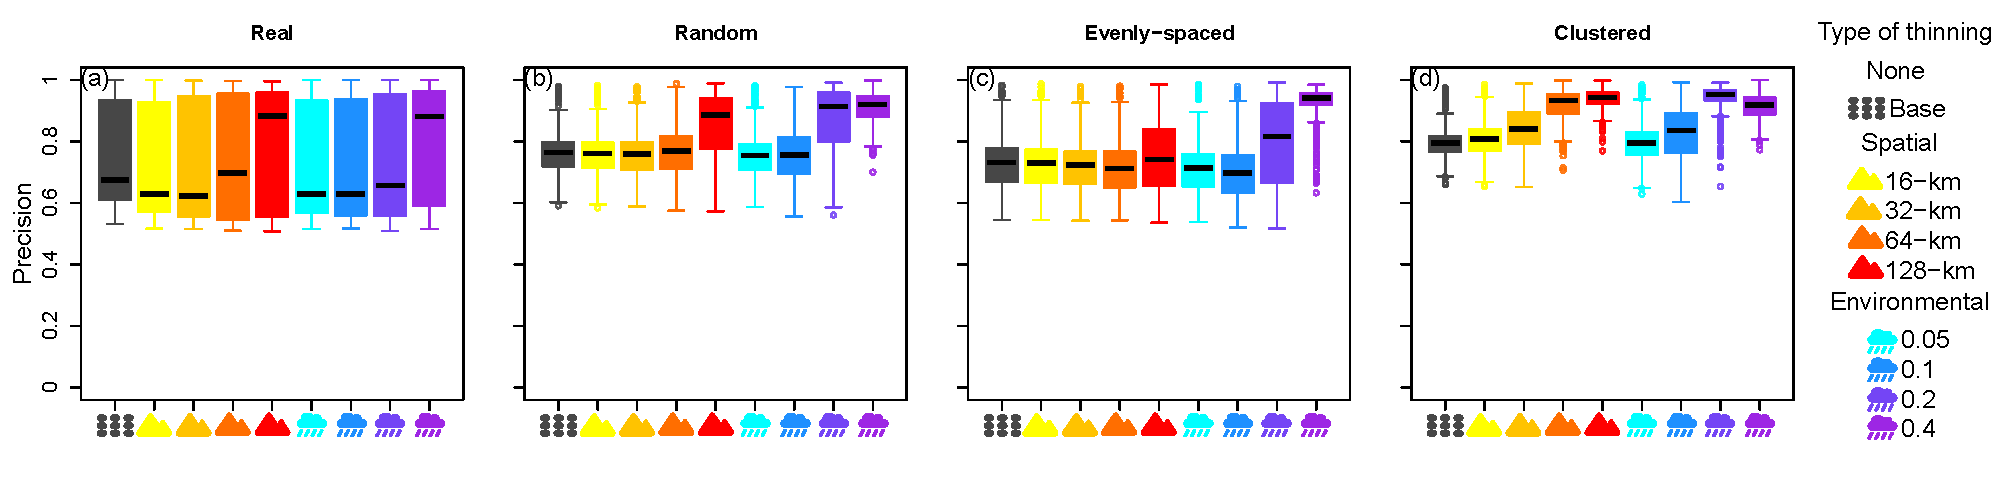
\includegraphics[width=1\textwidth]{Plots/FigureS17}} 
\caption[Effects of thinning on GAM precision]{The effects of spatial and environmental thinning on GAM precision of real species (a), and virtual species with random (b), clustered (c), and evenly-spaced (d) sampled occurrence points.}
 \label{fig:S17}
\end{figure}

\begin{figure}[h!]
\centering
%\graphicspath{ {c:/Teste/Chapter-1-Protocol/Manuscript/Plots/}  }
\centerline{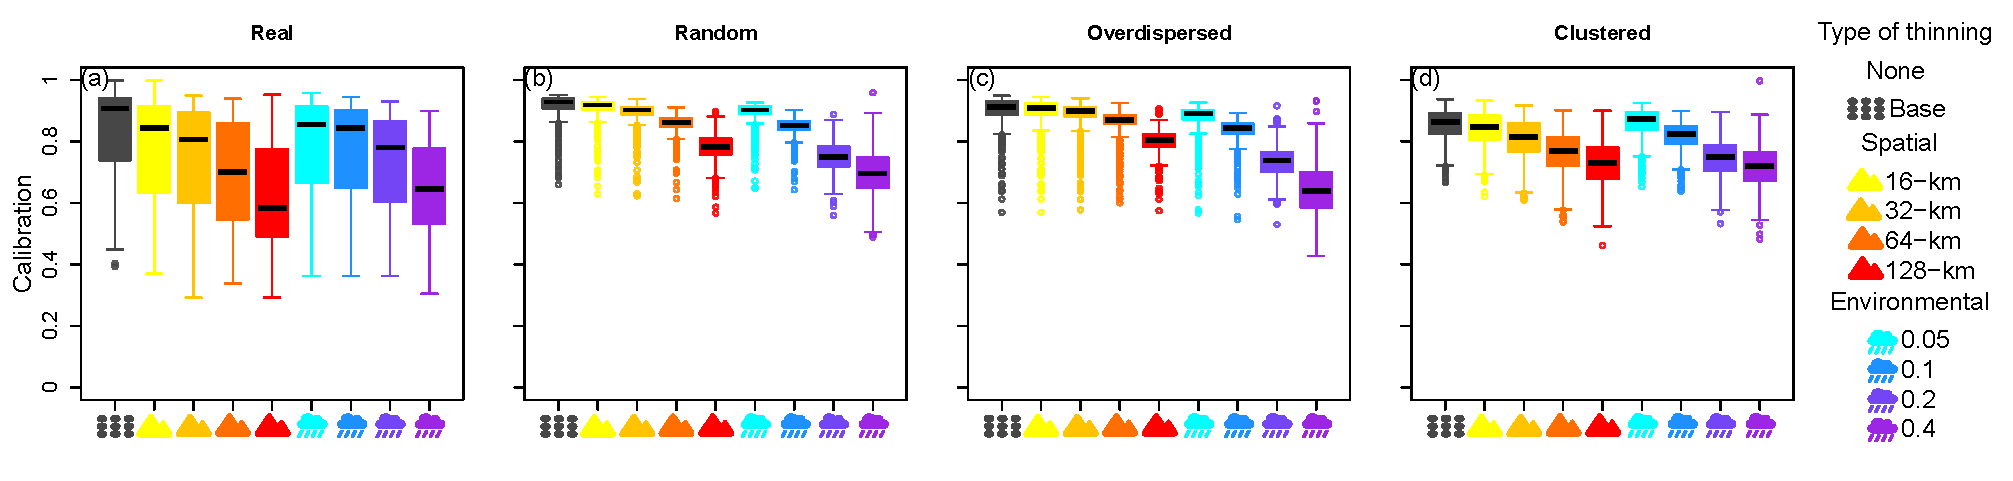
\includegraphics[width=1\textwidth]{Plots/FigureS18}} 
\caption[Effects of thinning on GAM calibration]{The effects of spatial and environmental thinning on GAM calibration of real species (a), and virtual species with random (b), clustered (c), and evenly-spaced (d) sampled occurrence points.}
 \label{fig:S18}
\end{figure}



\addtocontents{toc}{\protect\vskip-20pt}
\chapter{Supplemental information for Chapter 3}
\subsection*{\textbf{Lattice used to simulate population dynamics}}
The lattice used to simulate the population dynamics of the virtual species represented the United States and Canada and individuals could only occur within the borders of the lattice (black lines in Figure \ref{fig:NA_prec}). Although each species had a specific dispersal kernel with a particular combination of maximum and mean dispersal distances (e.g., Figure \ref{fig:kernel}), individuals could only disperse to cells within the limits of the lattice. Thus, if species occurred in a cell that was close to the border of the lattice, the species dispersal kernel was modified to allow individuals to disperse only to cells within the lattice (e.g., Figure \ref{fig:kern_crop}), preventing individuals from dispersing out of the lattice. We used mean annual temperature to generate two performance curves for each species that dictated how population growth rates changed along environmental gradients. Performance curves could be symmetric or asymmetric (left-skewed), but in both curves the species would achieve maximum growth rate under the same environmental conditions though growth rates deteriorated differently away from this optimum in each curve (Figure \ref{fig:curves}). The wide range of temperature values in the United States and Canada allowed the simulation of a variety of performance curves with different characteristics (i.e., breadths and optimum) for our virtual species. 

\begin{figure}[H]
\centering
\centerline{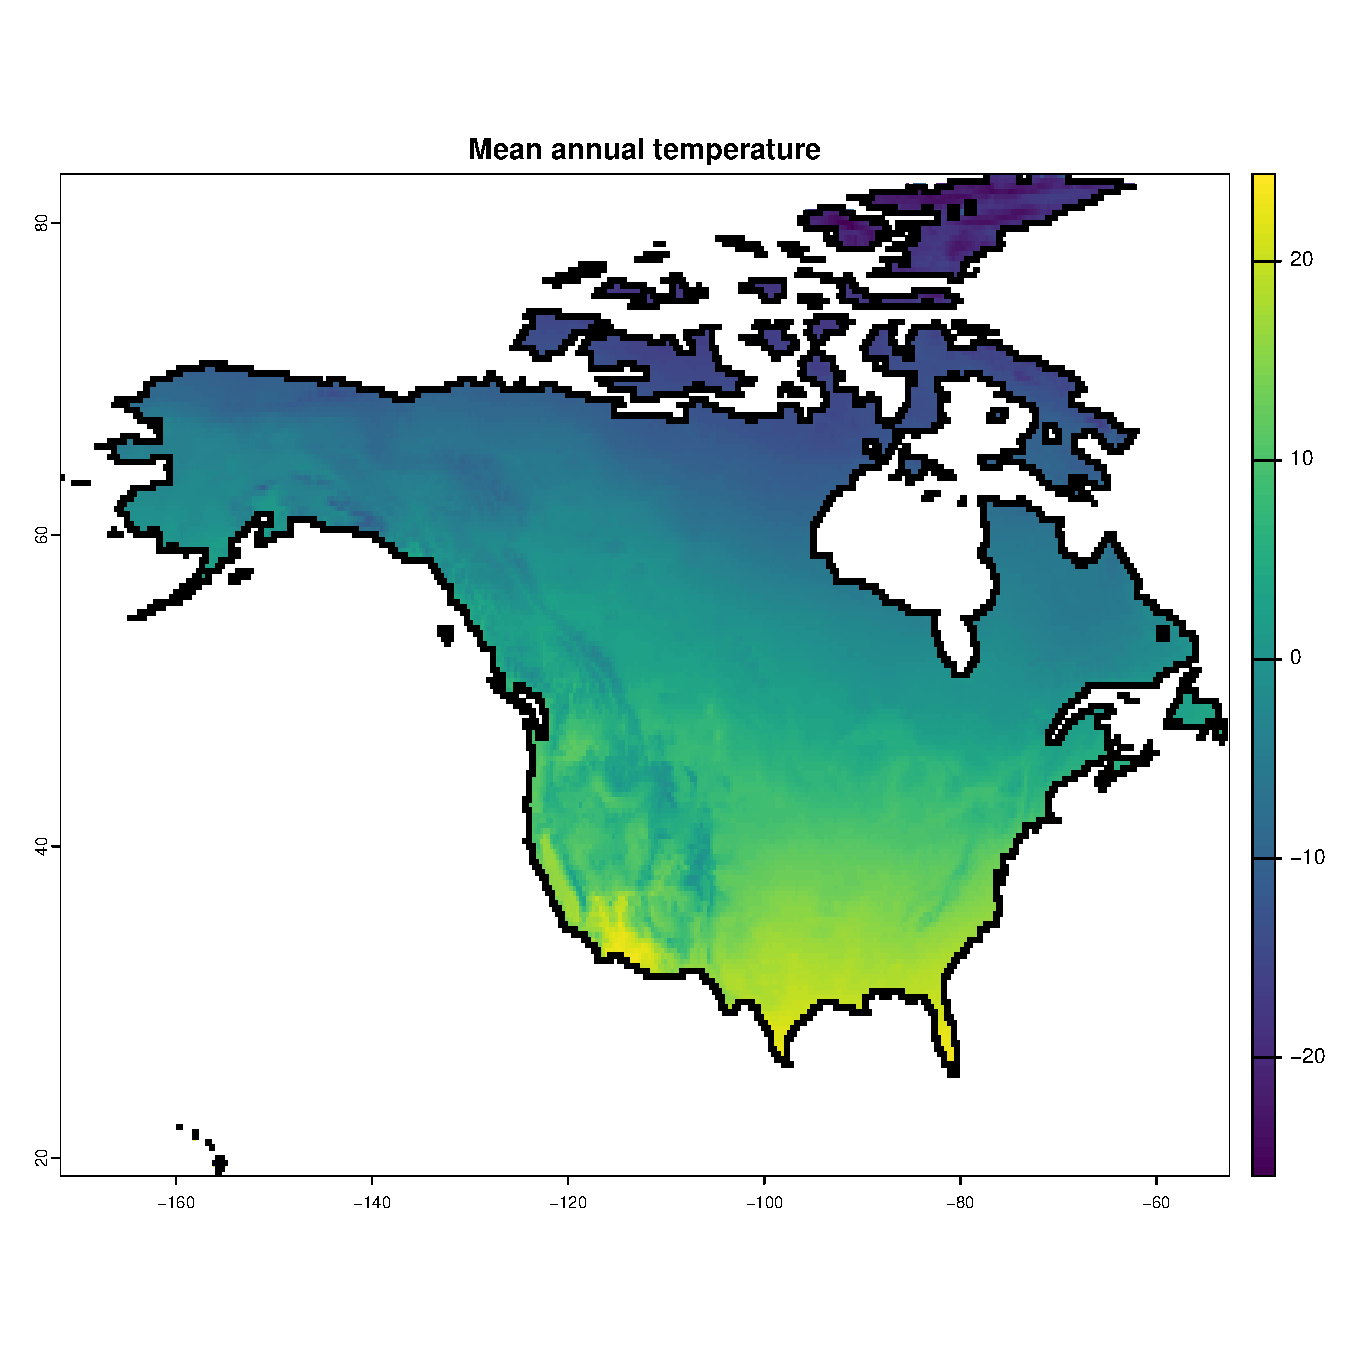
\includegraphics[width=1\textwidth]{FigsdmAbnd/NA_prec}}
\caption[Mean annual temperature in North America]{We used a lattice that had information on mean annual temperature in the United States and Canada to simulate population dynamics. Mean annual temperature values ranged from -26-24.4 $^{\circ}$C, allowing the possibility of simulating species that exist under a broad variety of environments.} 
\label{fig:NA_prec}
\end{figure}

\begin{figure}[H]
\centering
\centerline{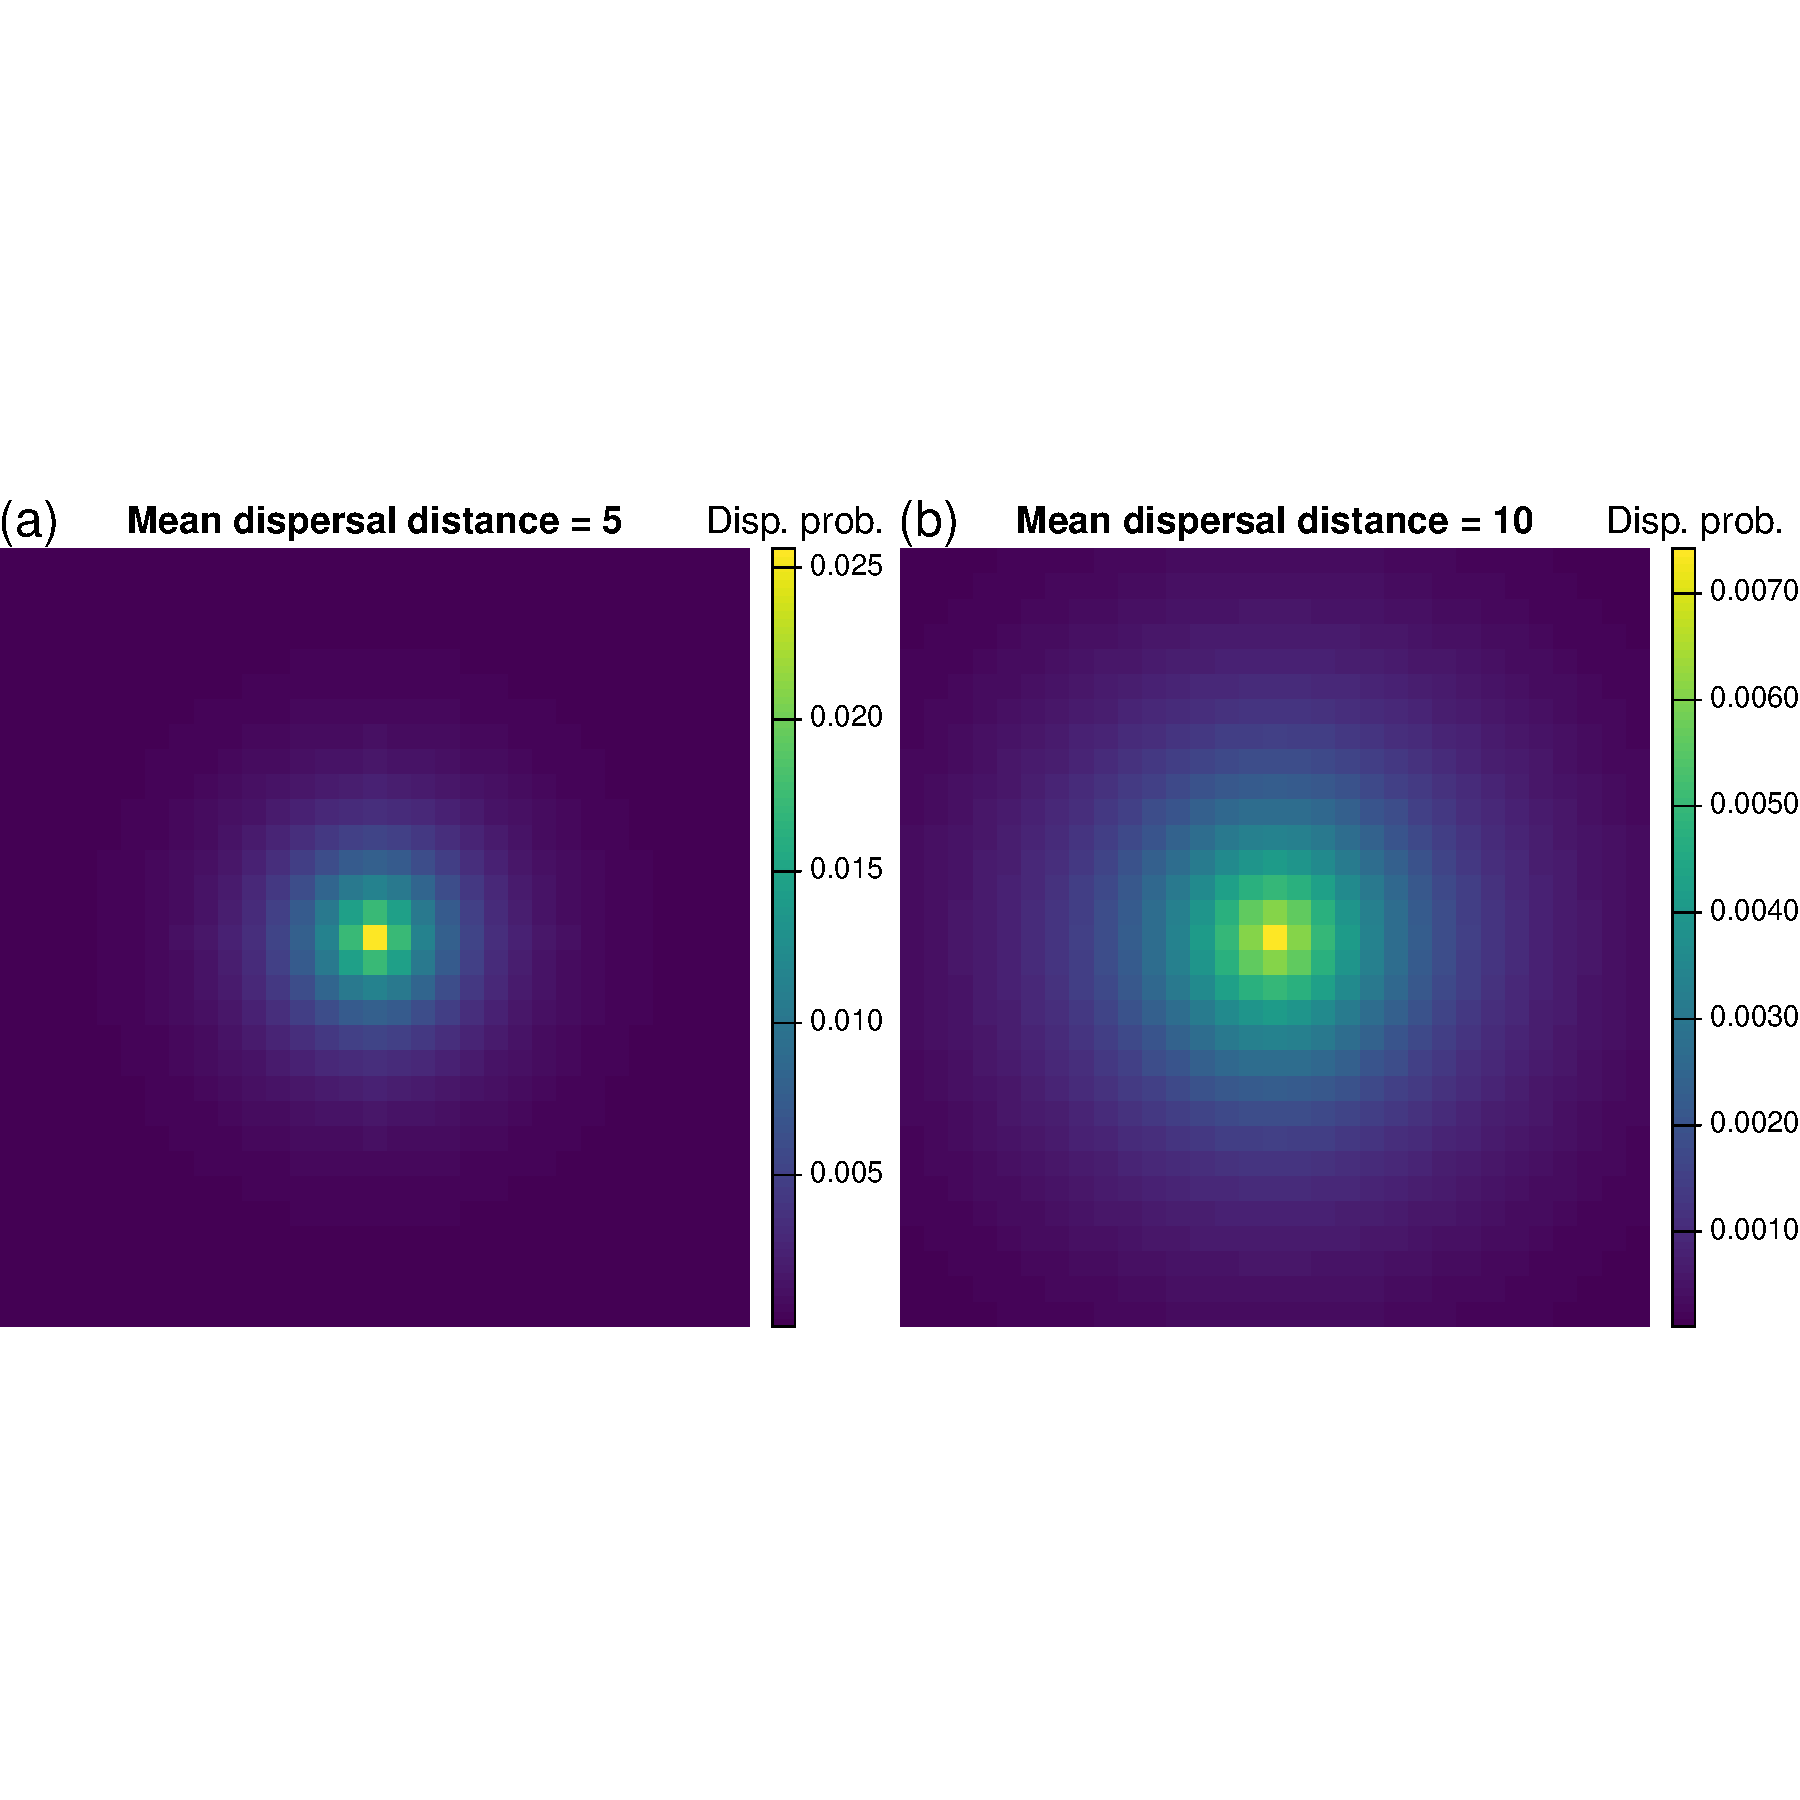
\includegraphics[width=1\textwidth]{FigsdmAbnd/kernels}}
\caption[Dispersal kernel]{A negative exponential dispersal kernel was used to simulate the dispersal of individuals between populations where each species had a dispersal kernel with specific maximum and mean dispersal distances to consider dispersal differences between species.} 
\label{fig:kernel}
\end{figure}


\begin{figure}[H]
\centering
\centerline{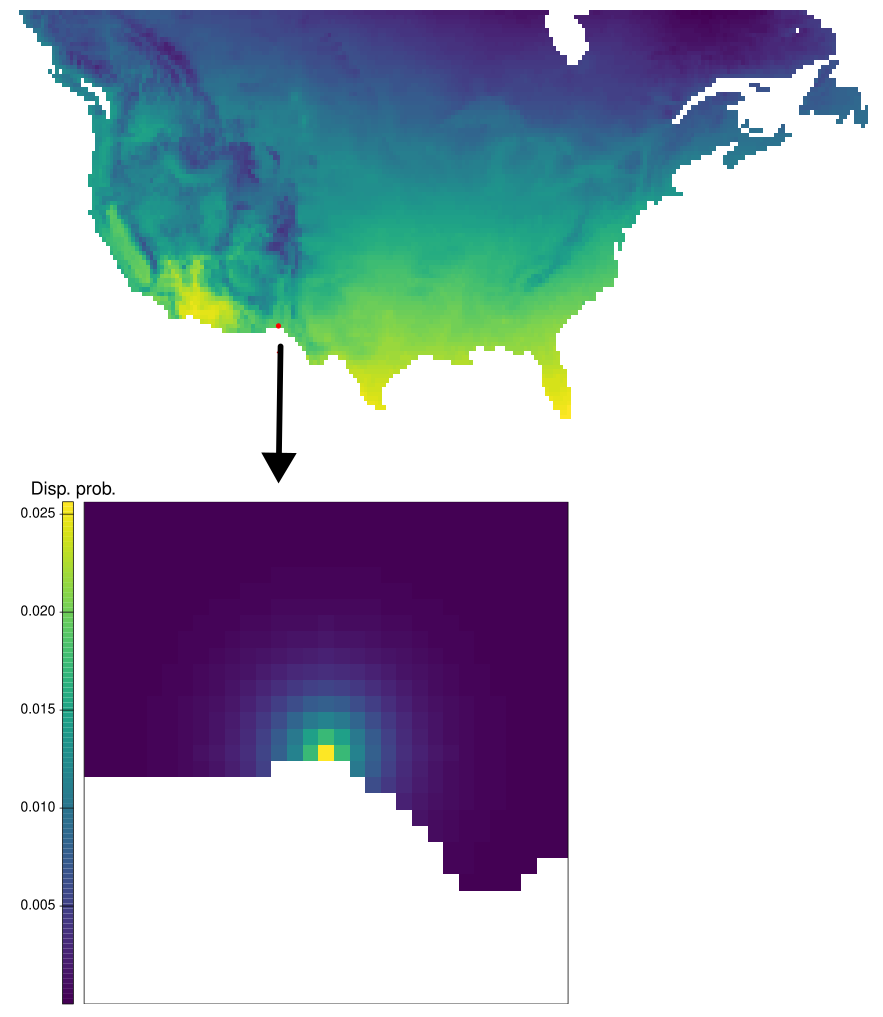
\includegraphics[width=1\textwidth]{FigsdmAbnd/kernel_crop_na.png}}
\caption[Cropped dispersal kernel]{Individuals dispersing from populations could only migrate to cells that were within the borders of the lattice representing the United States and Canada. To achieve that, only the cells of the dispersal kernel that were within United States and Canada had dispersal probabilities associated with them.} 
\label{fig:kern_crop}
\end{figure}


\begin{figure}[H]
\centering
\centerline{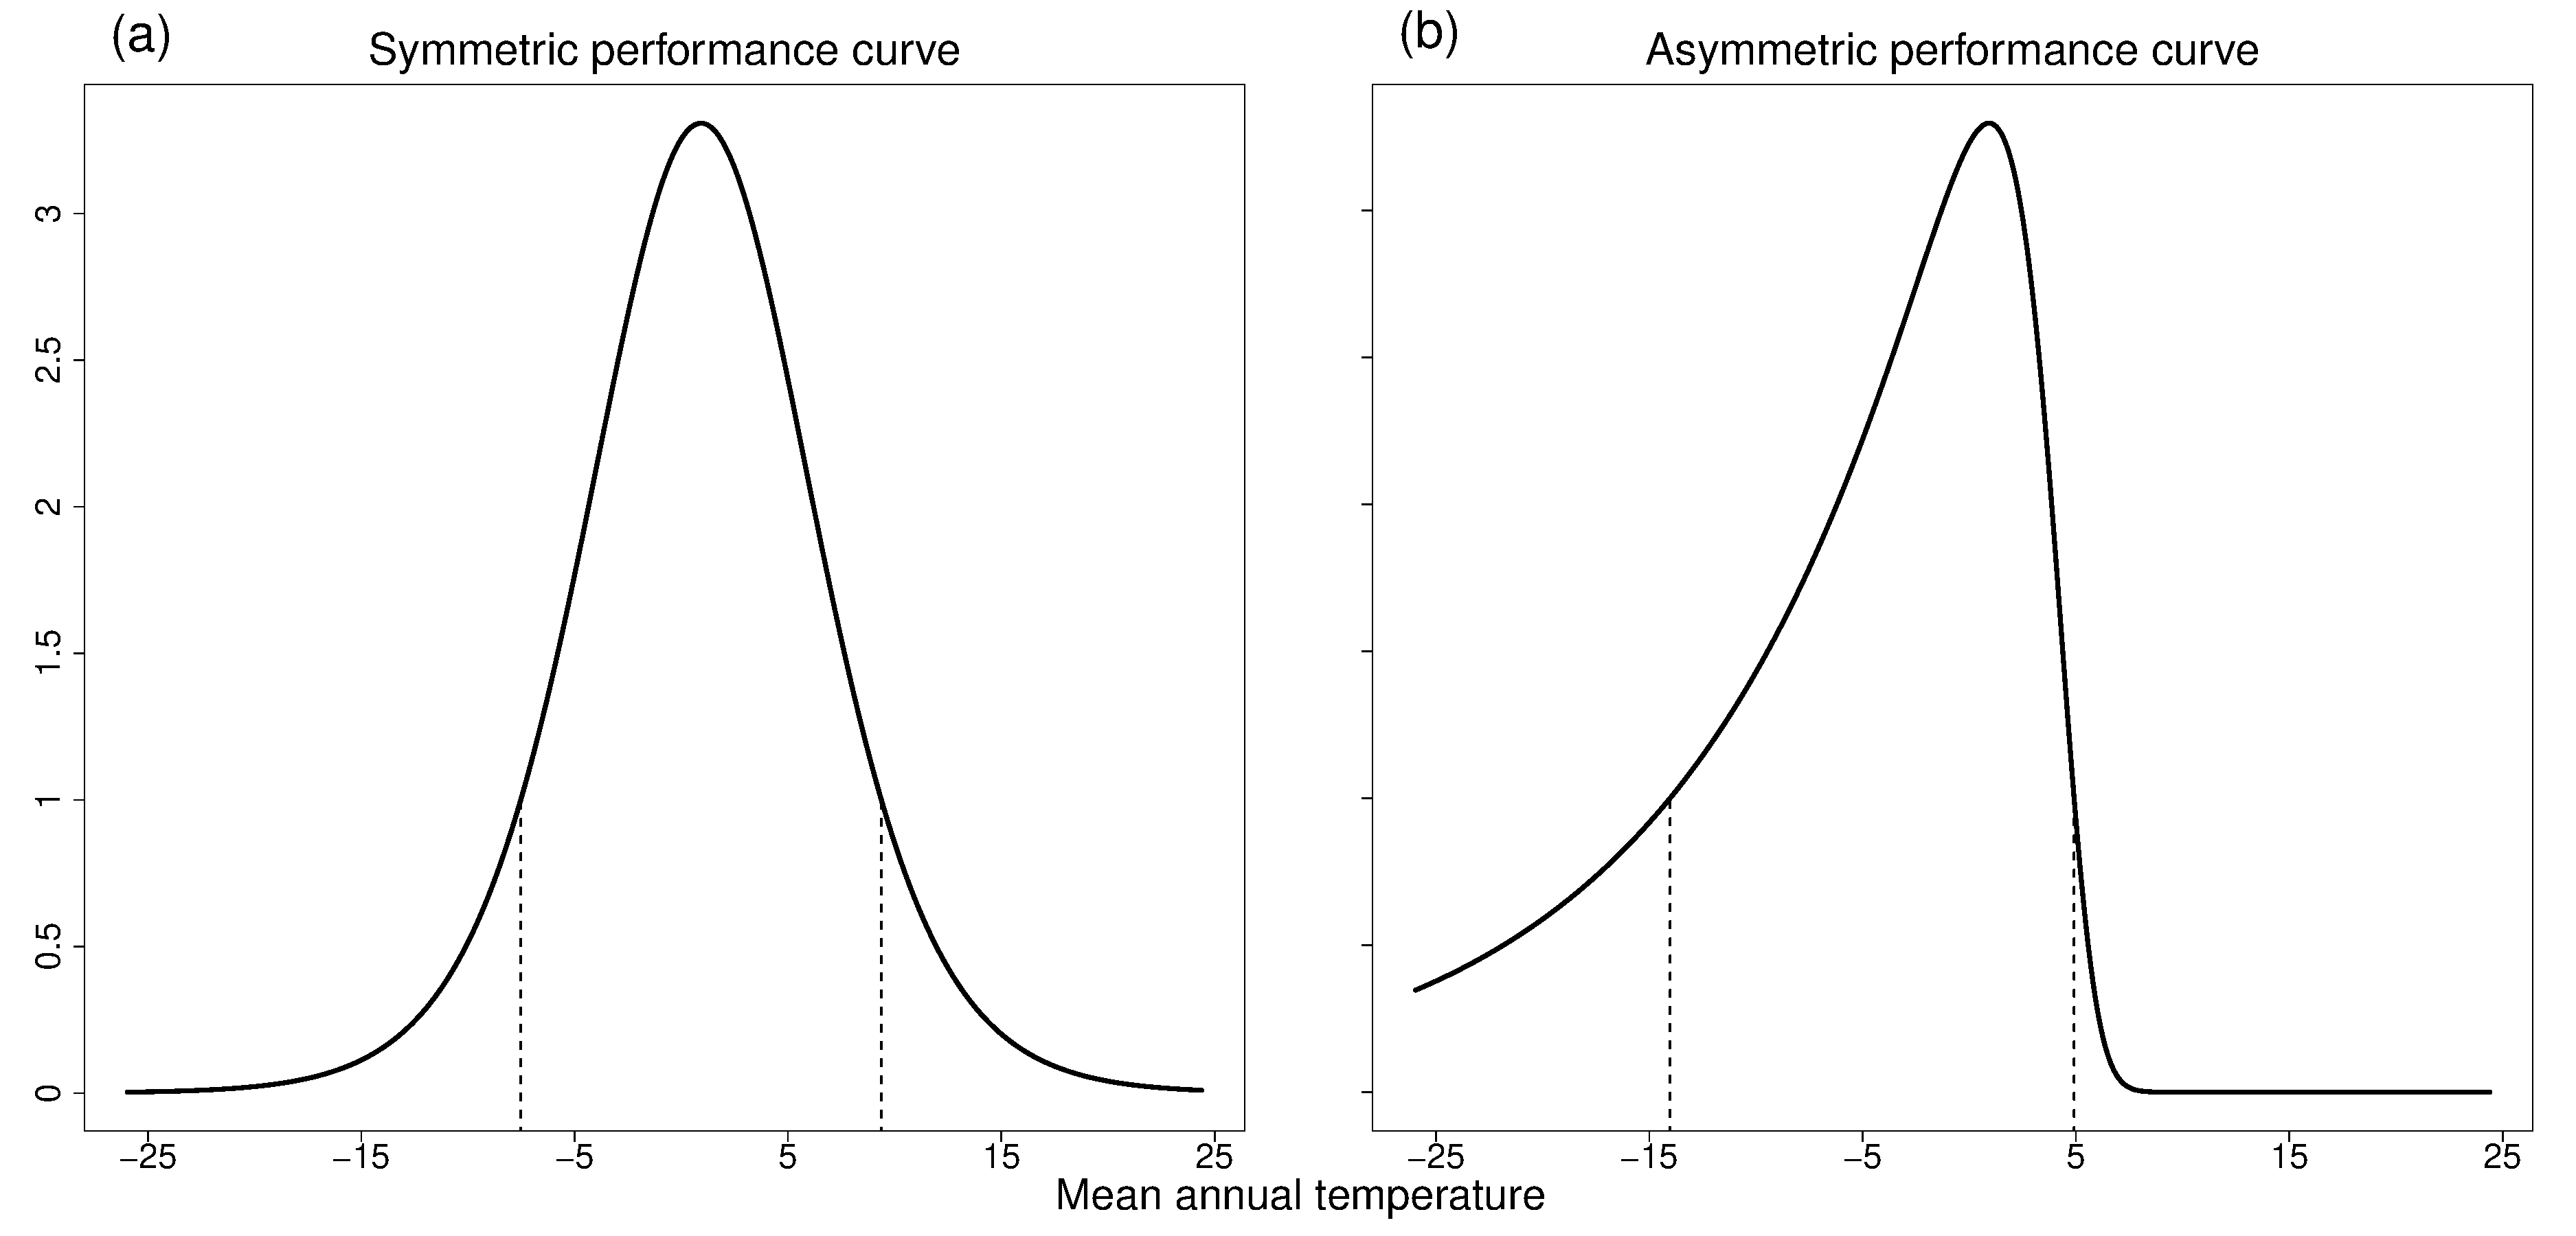
\includegraphics[width=1\textwidth]{FigsdmAbnd/performances}}
\caption[Symmetric and asymmetric performance curves]{Symmetric (a) and asymmetric (b) performance curves for a species that had an optimum mean annual temperature of 0.93 $^{\circ}$C. Dashed lines represent the range of temperatures where population growth rate is above 1 for both performance curves. } 
\label{fig:curves}
\end{figure}

\subsection*{\textbf{Linear mixed effect models diagnostic}}
Model diagnostics for the linear mixed models that we fit were done using the \texttt{performance} R package. Visual checks on the family used for our response variable, the linearity and normality of the residuals, the homogeneity of the variance, the collinearity of the predictor variables, and the normality of the random effects were performed. These visual checks indicated that these model assumptions were generally met (Figures \ref{fig:mod_dyn}-\ref{fig:mod_sp}), suggesting that our results are robust. 

\begin{figure}[H]
\centering
\centerline{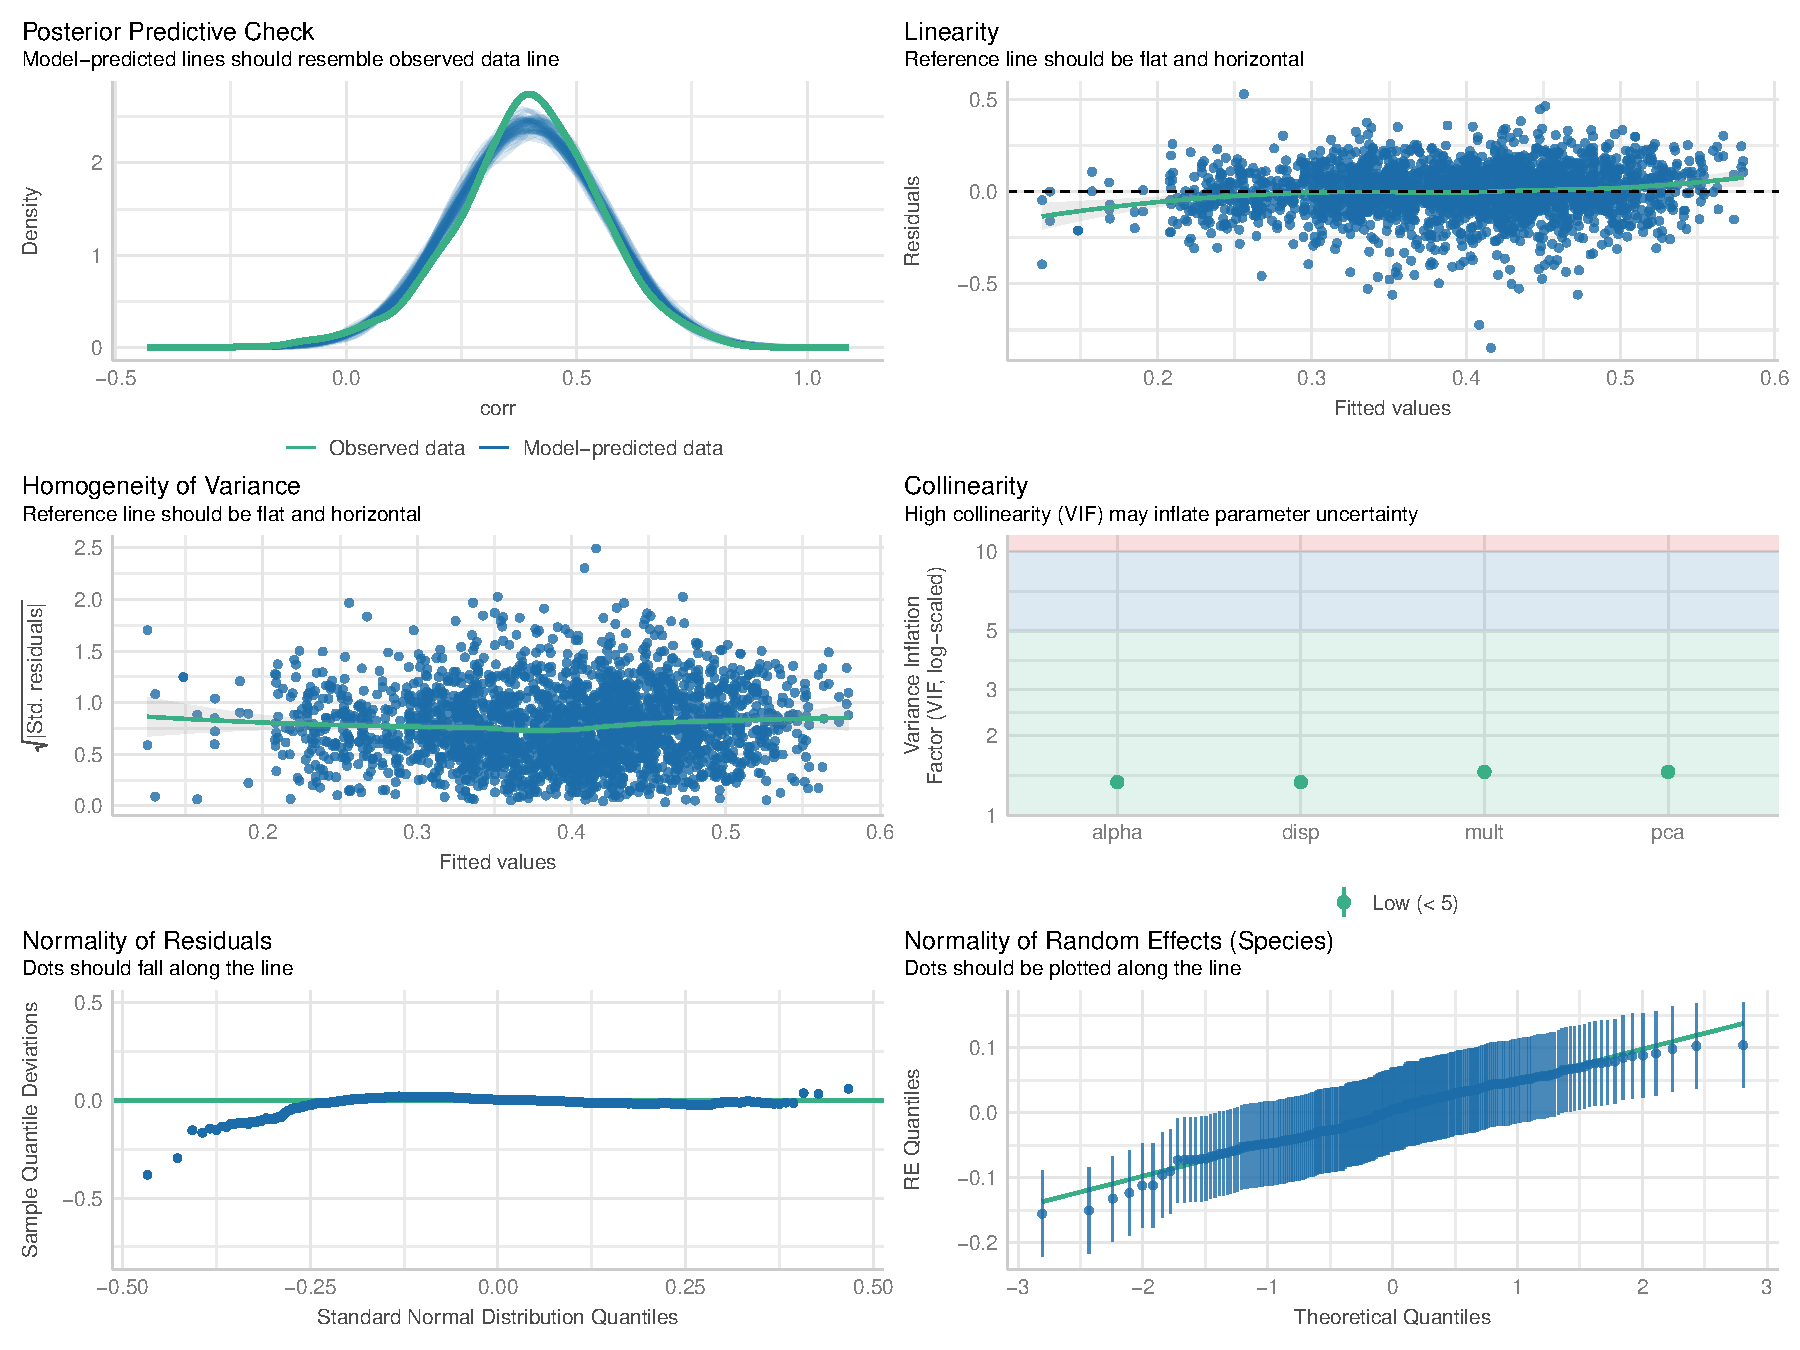
\includegraphics[width=1\textwidth]{FigsdmAbnd/mod_dyn}}
\caption[Model diagnostics for population dynamics]{Visual model diagnostics for our first linear mixed effect models presented in Figure \ref{fig:cor}. Overall, the gaussian family fits well to the response variable that we used in the models (corr), the linearity assumption is met, variance is homogeneous, there is not correlation between the predictor variables (i.e., variance inflation factor (VIF) < 5), and the residuals and the random effects are normally distributed.} 
\label{fig:mod_dyn}
\end{figure}

\begin{figure}[H]
\centering
\centerline{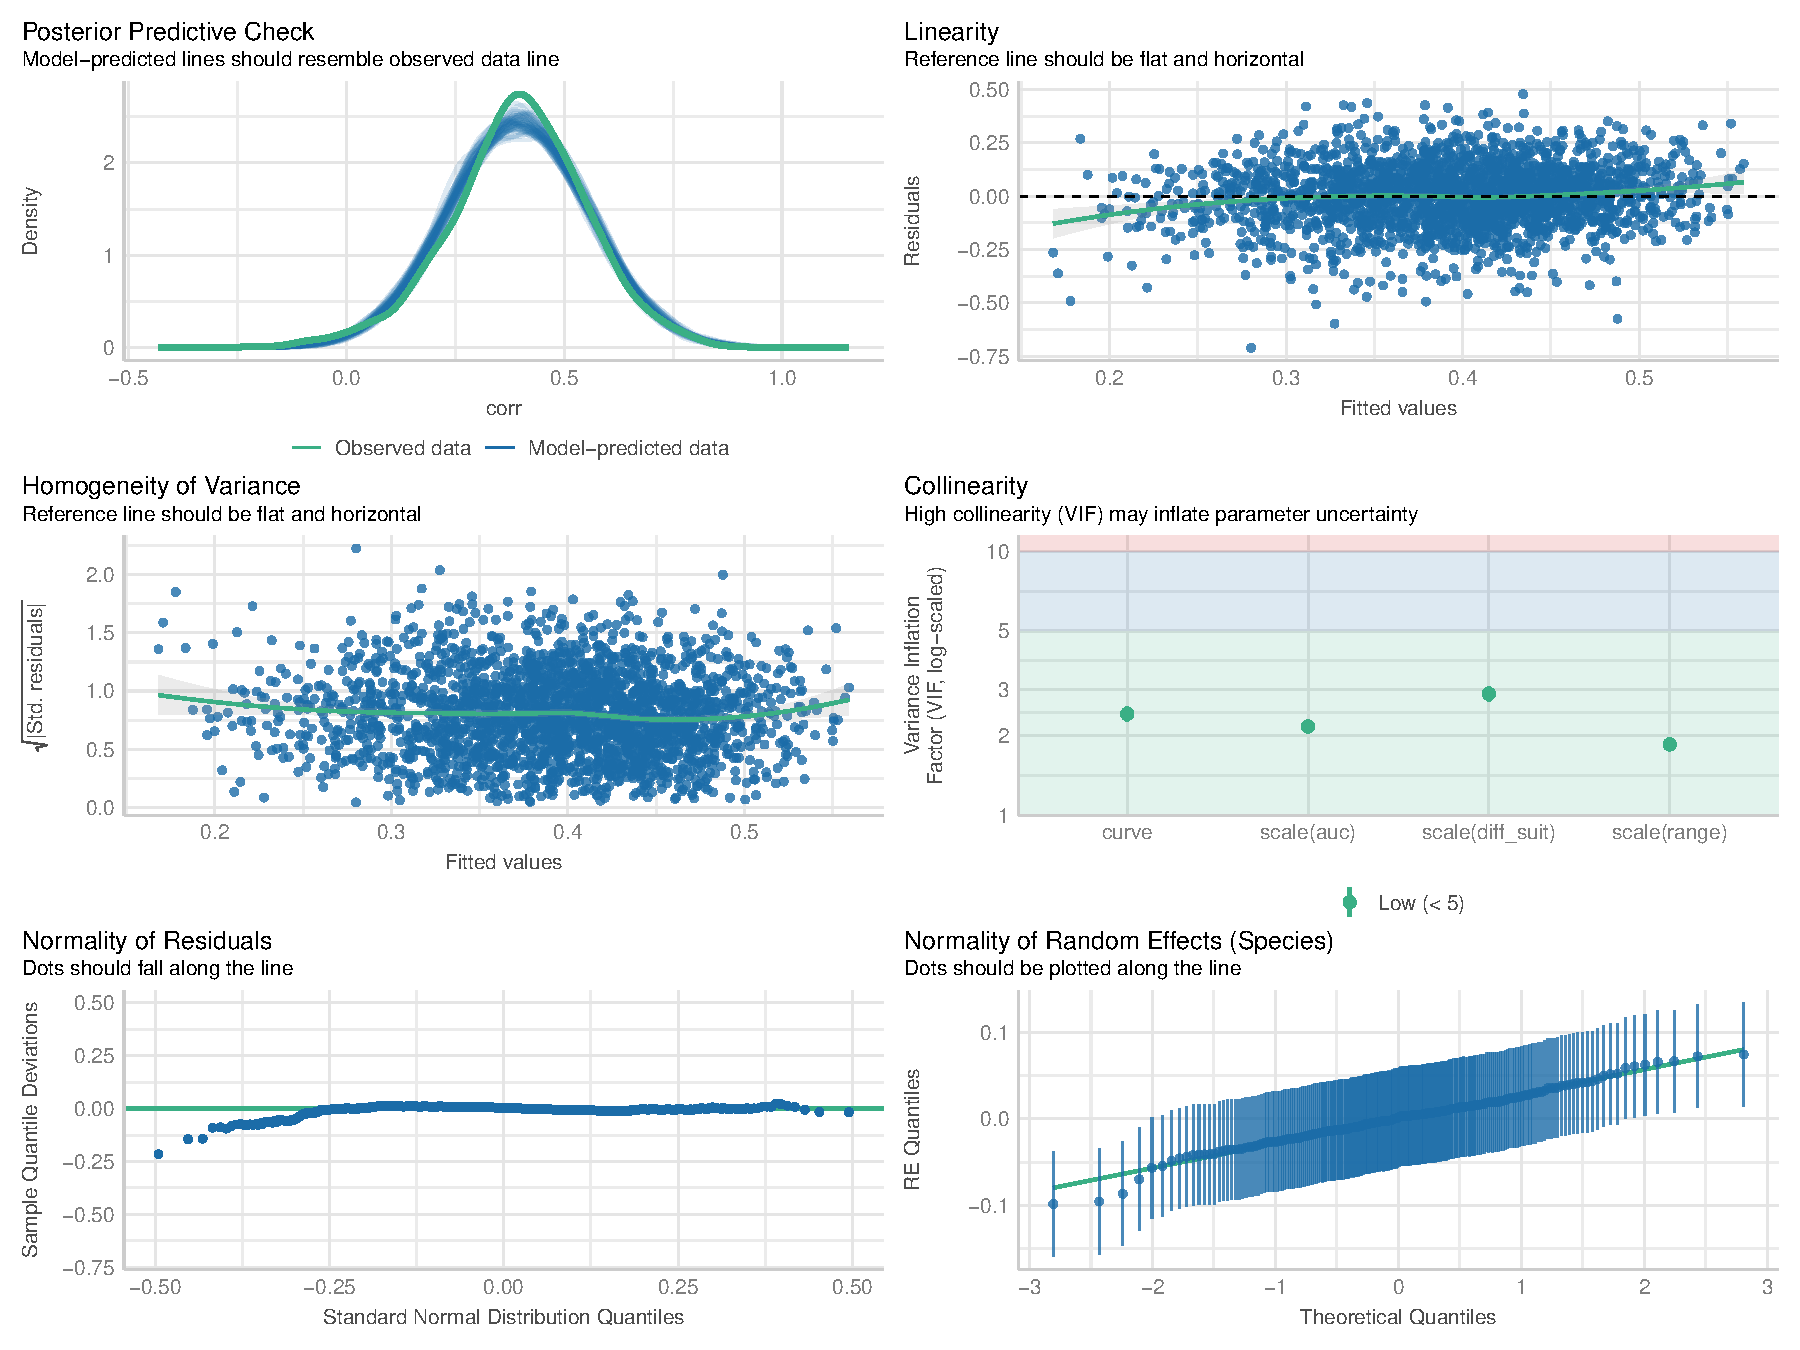
\includegraphics[width=1\textwidth]{FigsdmAbnd/mod_sp}}
\caption[Model diagnostics for species differences]{Visual model diagnostics for our second linear mixed effect models presented in Figure \ref{fig:diff}. Overall, the gaussian family fits well to the response variable that we used in the models (corr), the linearity assumption is met, variance is homogeneous, there is not correlation between the predictor variables (i.e., variance inflation factor (VIF) < 5), and the residuals and the random effects are normally distributed.} 
\label{fig:mod_sp}
\end{figure}


\subsection*{\textbf{Species distribution performance}}
The performance (AUC) of SDMs was affected by whether dispersal was considered when simulating the population dynamics of virtual species (Figure \ref{fig:auc}a). Mean performance was 0.68 and 0.72 for SDMs that were trained with occurrence data obtained from population models that considered only demographic stochasticity or demographic stochasticity and spatial variation in the strength of intraspecific competition respectively. Mean performances ranged from 0.59-0.64 for all population models that included the occurrence of dispersal events, showing a significant decrease in performance compared to when dispersal was not considered. Such decrease in SDM performance probably occurred due to the fact that, when dispersal is allowed, sink populations can be sampled and used to model the species distributions. In this case, SDM might not be able to properly detect sink populations from occurrence data, and consequently areas that are environmentally unsuitable for the species can be labeled as suitable by SDM and negatively affect performance during model evaluation. There is a negative correlation ($r$ = -0.53, $p > 0.01$; Figure \ref{fig:auc}b) between the breadth of species performance curves and SDM performance, suggesting an inability of SDMs to properly estimate the distribution of generalist species. Mean SDM performance for North American birds was 0.83. 


\begin{figure}[H]
\centering
\centerline{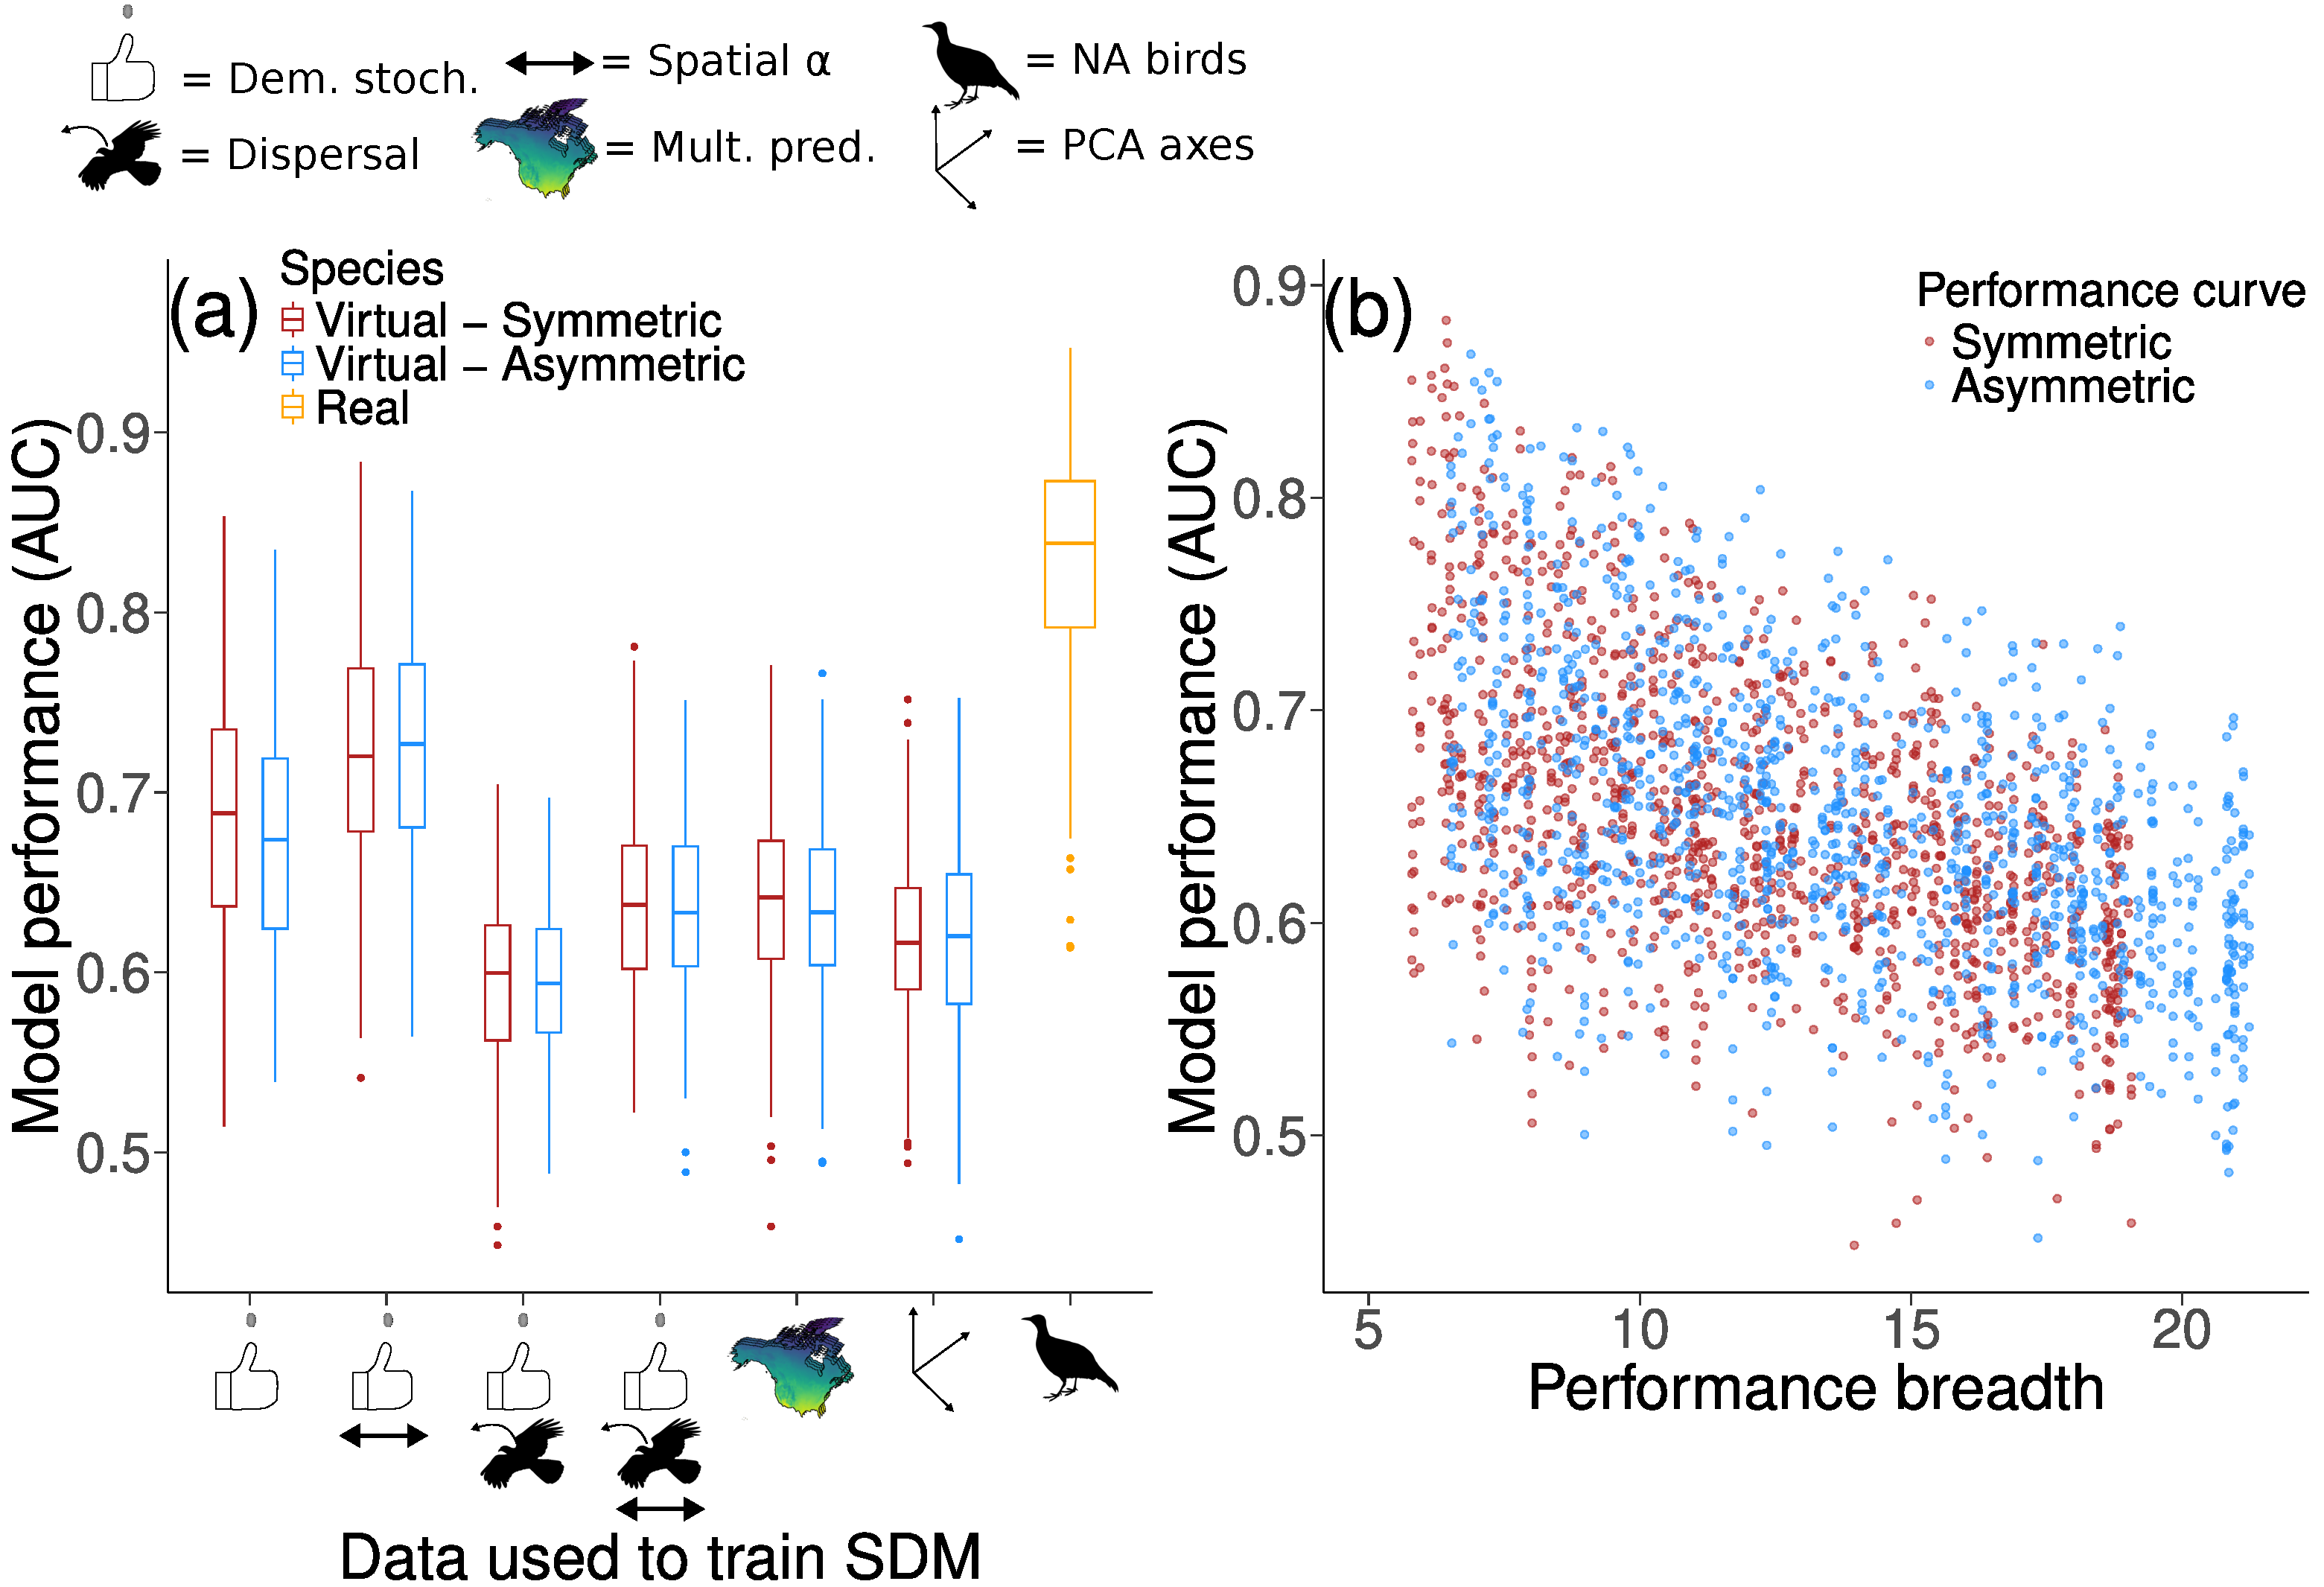
\includegraphics[width=1\textwidth]{FigsdmAbnd/Vioauc}}
\caption[Species distribution model performance]{Average model performance (AUC) observed for virtual species with symmetric and asymmetric performance curves and for North American birds.} 
\label{fig:auc}
\end{figure}

\subsection*{\textbf{Variable importance}}
SDMs that were trained with mean annual temperature and NDVI as predictors consistently identified mean annual temperature as the most important variable determining species occurrence (mean importance ranged from 79-92\%, Figure \ref{fig:imp}). When multiple environmental predictors were used to train SDM, the mean variable importance for mean annual temperature was 61\%, showing a decrease in the ability of these models in convincingly detecting the environmental condition that drives species occurrence when several environmental predictors are added to the model.


\begin{figure}[ht]
\centering
\centerline{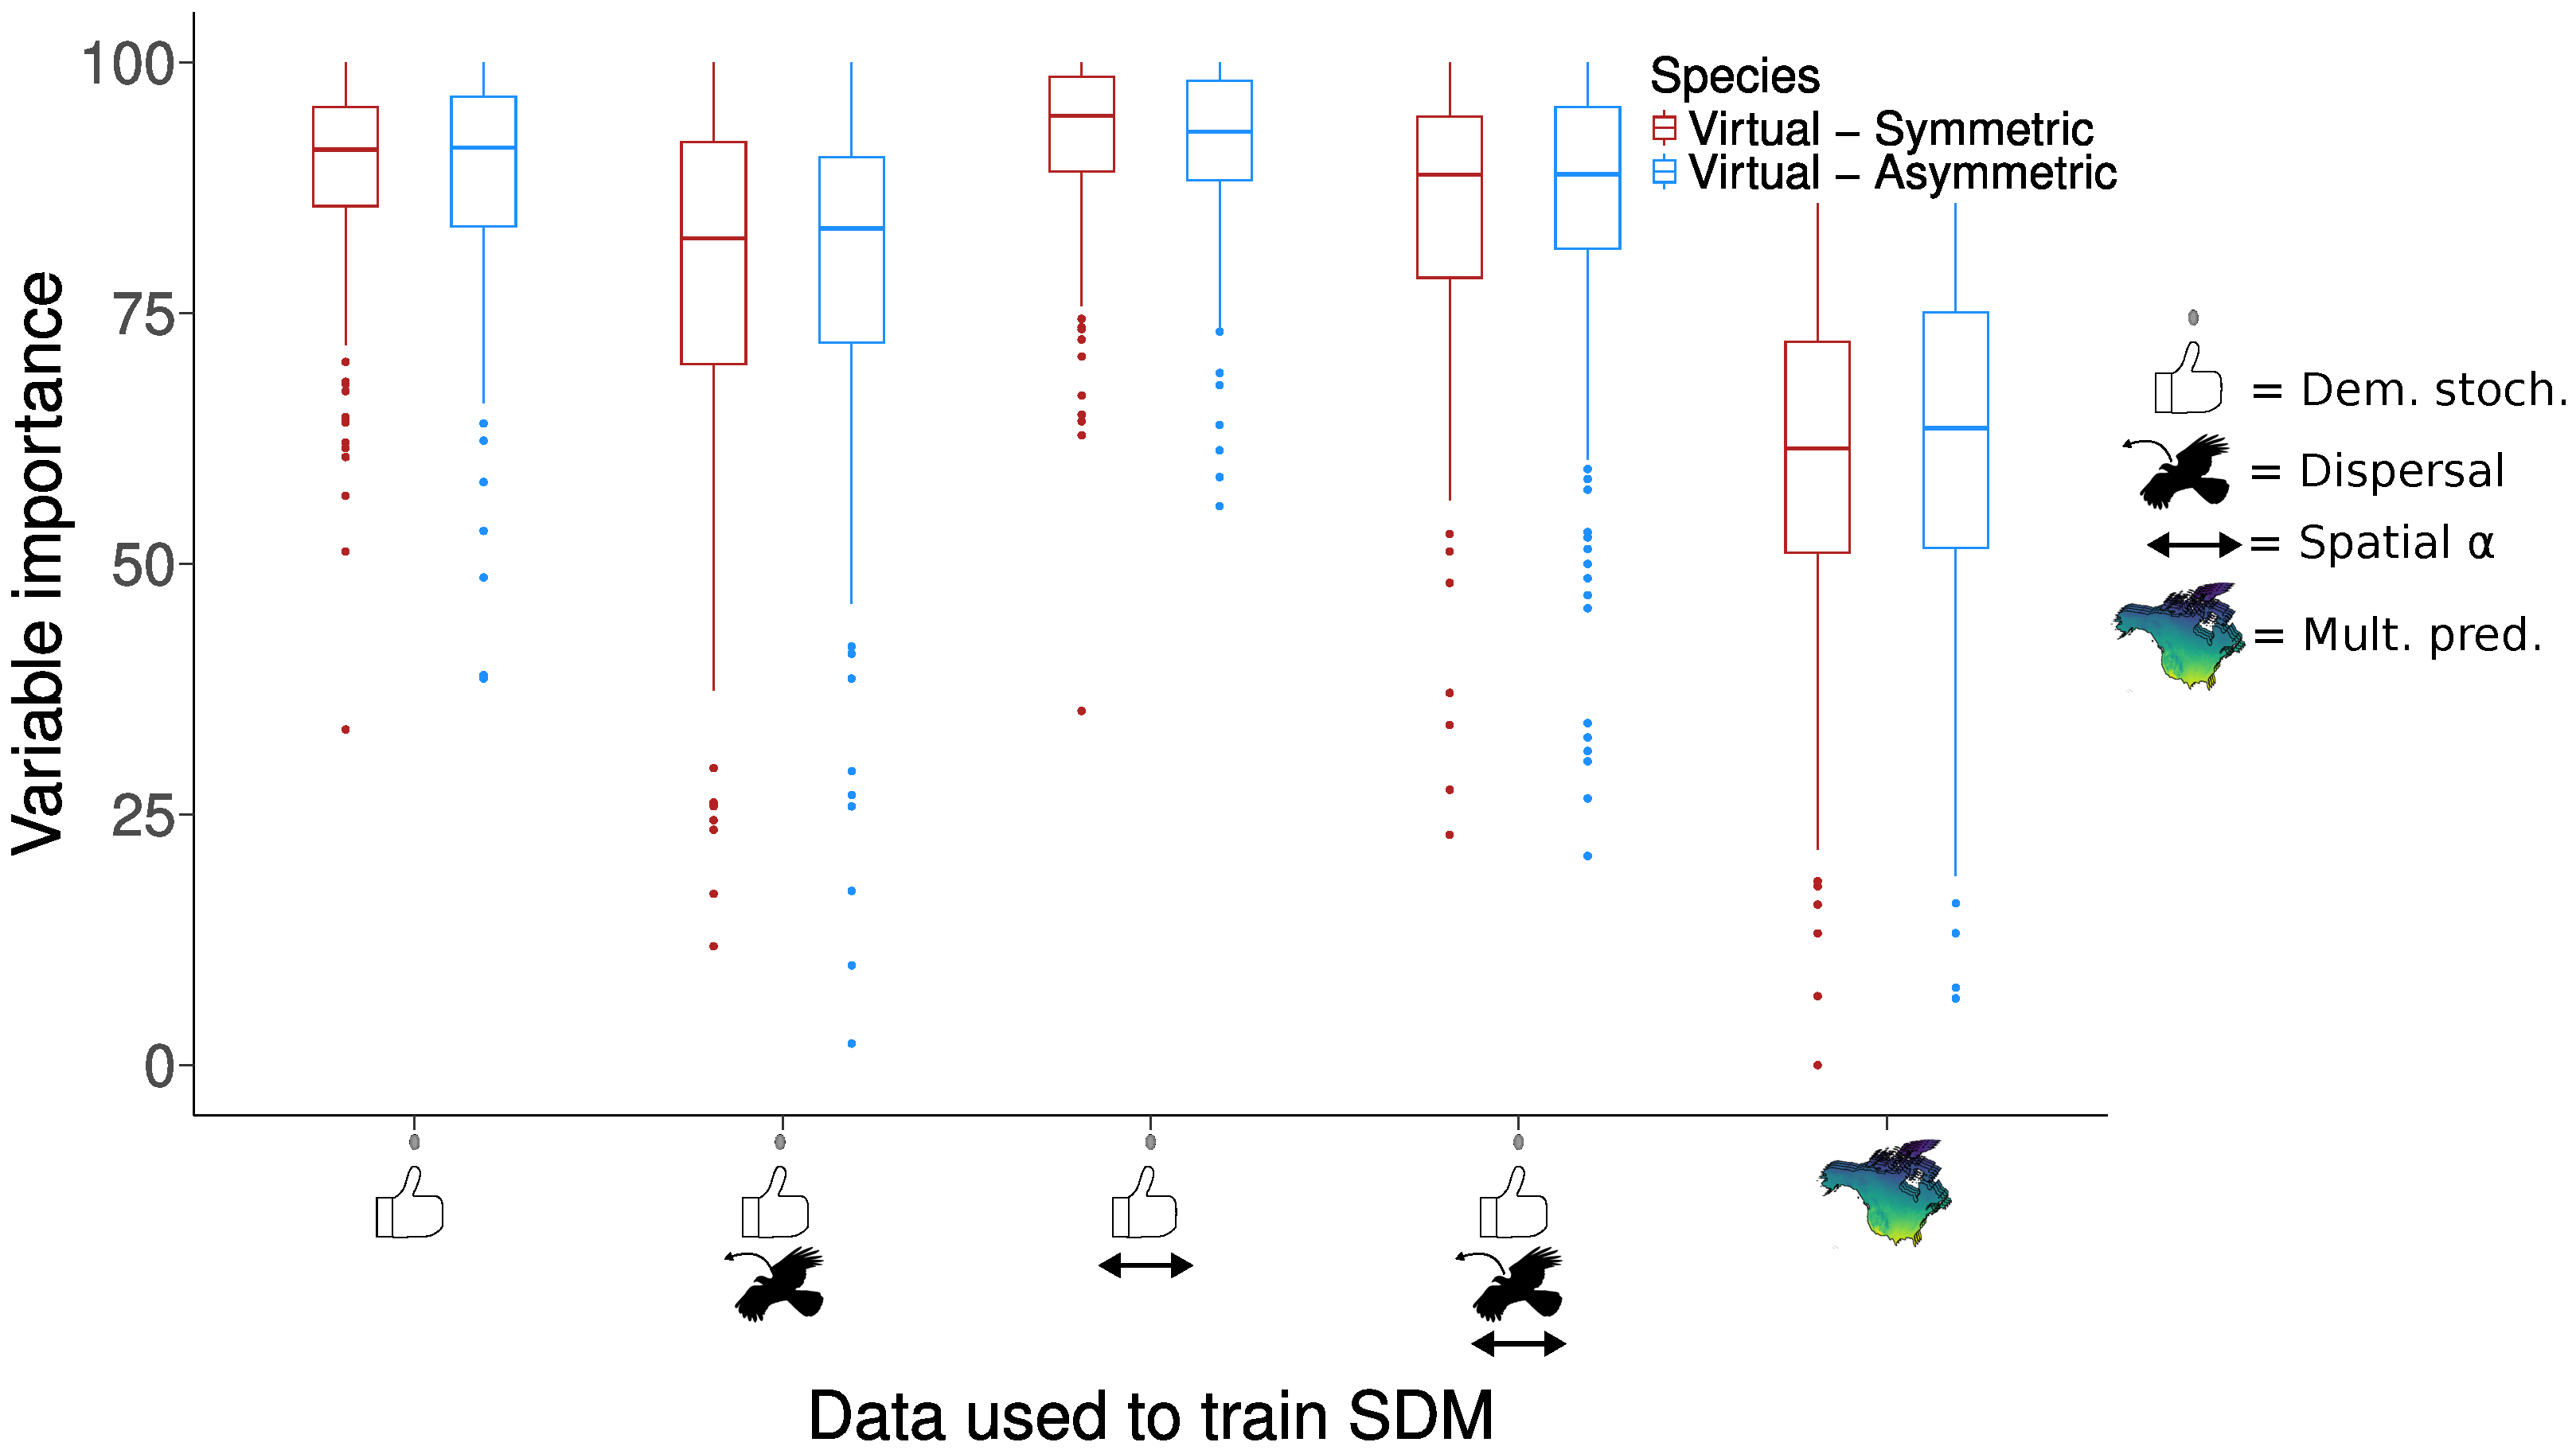
\includegraphics[width=1\textwidth]{FigsdmAbnd/impBox}}
\caption[Variable importance]{Variable importance (\%) score for mean annual temperature observed for virtual species with symmetric and asymmetric performance curves that had populations simulated considering different combinations of demographic stochasticity, spatial variation in the strength of intraspecific competition and dispersal.} 
\label{fig:imp}
\end{figure}
                        %% command \Appendix or \Appendices
\addtocontents{toc}{\protect\vskip-20pt}
\chapter{Supplemental information for Chapter 5}
\section*{\textbf{Resident North American birds range limits}}
We estimated the geographic range limits of the 96 resident North American birds used in our analyses that had geographic ranges in birdLife. Overall, species commonly have geographic range limits that represent the terrestrial boundaries of North America (Figure \ref{fig:rangelimits}), suggesting that range limits may often not represent niche limits. 

\begin{figure}[H]
\centering
\centerline{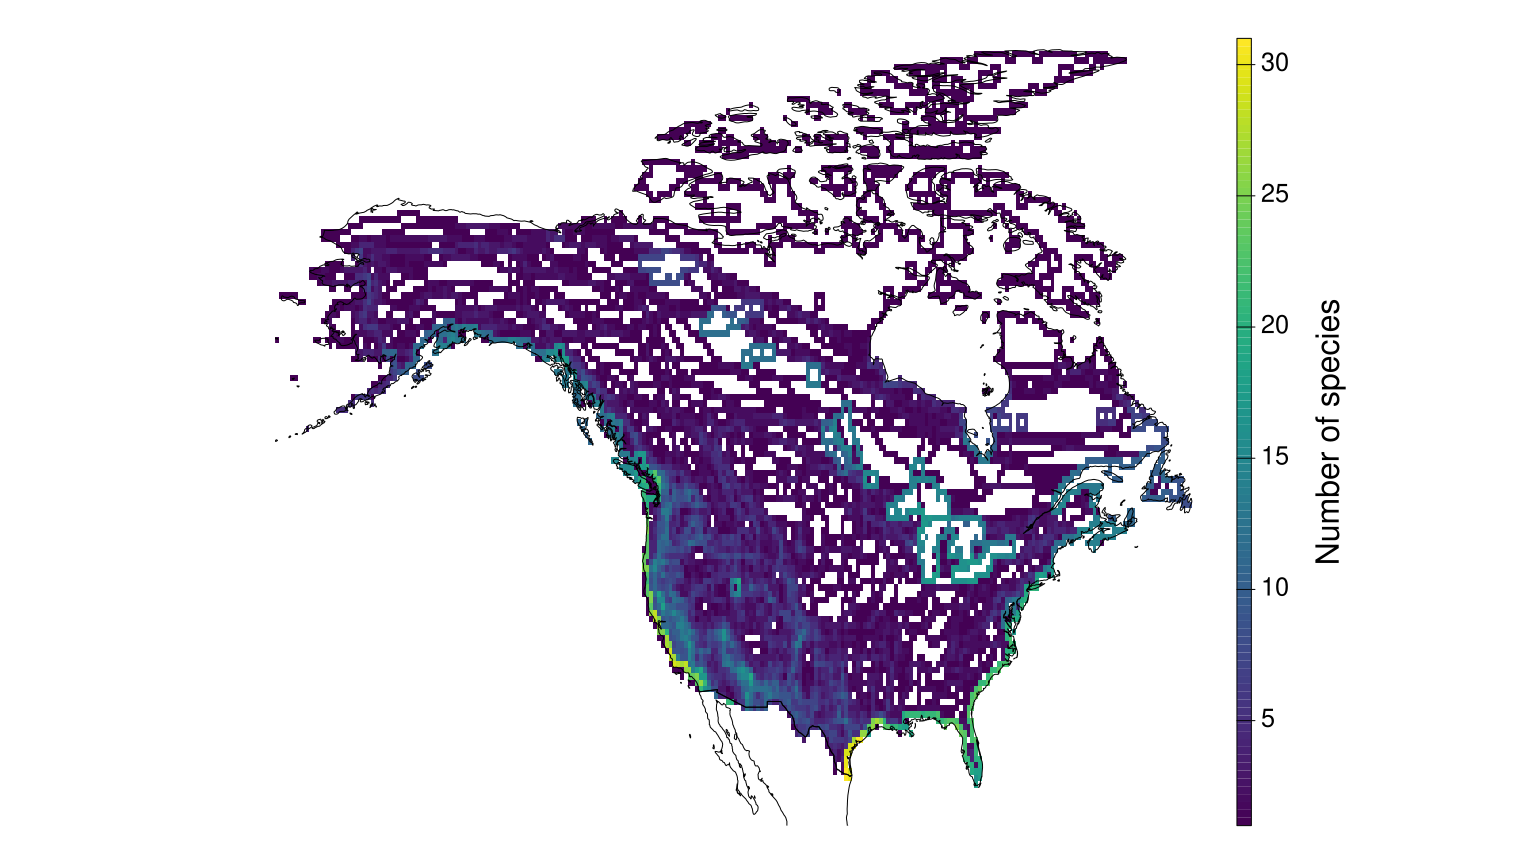
\includegraphics[width=1\textwidth]{FigRange/rangelimits.png}}
\caption[Geographic range limits]{Geographic range limits of 96 resident North American birds that have expert geographic ranges. Species more often have geographic range limits near the terrestrial borders of North America than within the continent, indicating that geographic ranges of several species may not be limited by their climatic niche. The colors represent the number of species that have geographic range edges in a given location.}  
\label{fig:rangelimits}
\end{figure}
\section*{\textbf{Sites sampled by the Breeding Bird Survey}}
The species considered in our study were observed in a total of 4803 routes that were sampled between 1997 and 2019 by the BBS. About 3051$\pm$127 routes were sampled annually and routes were sampled on average for 15$\pm$7 years (Figure \ref{fig:routes}). 
\begin{figure}[H]
\centering
\centerline{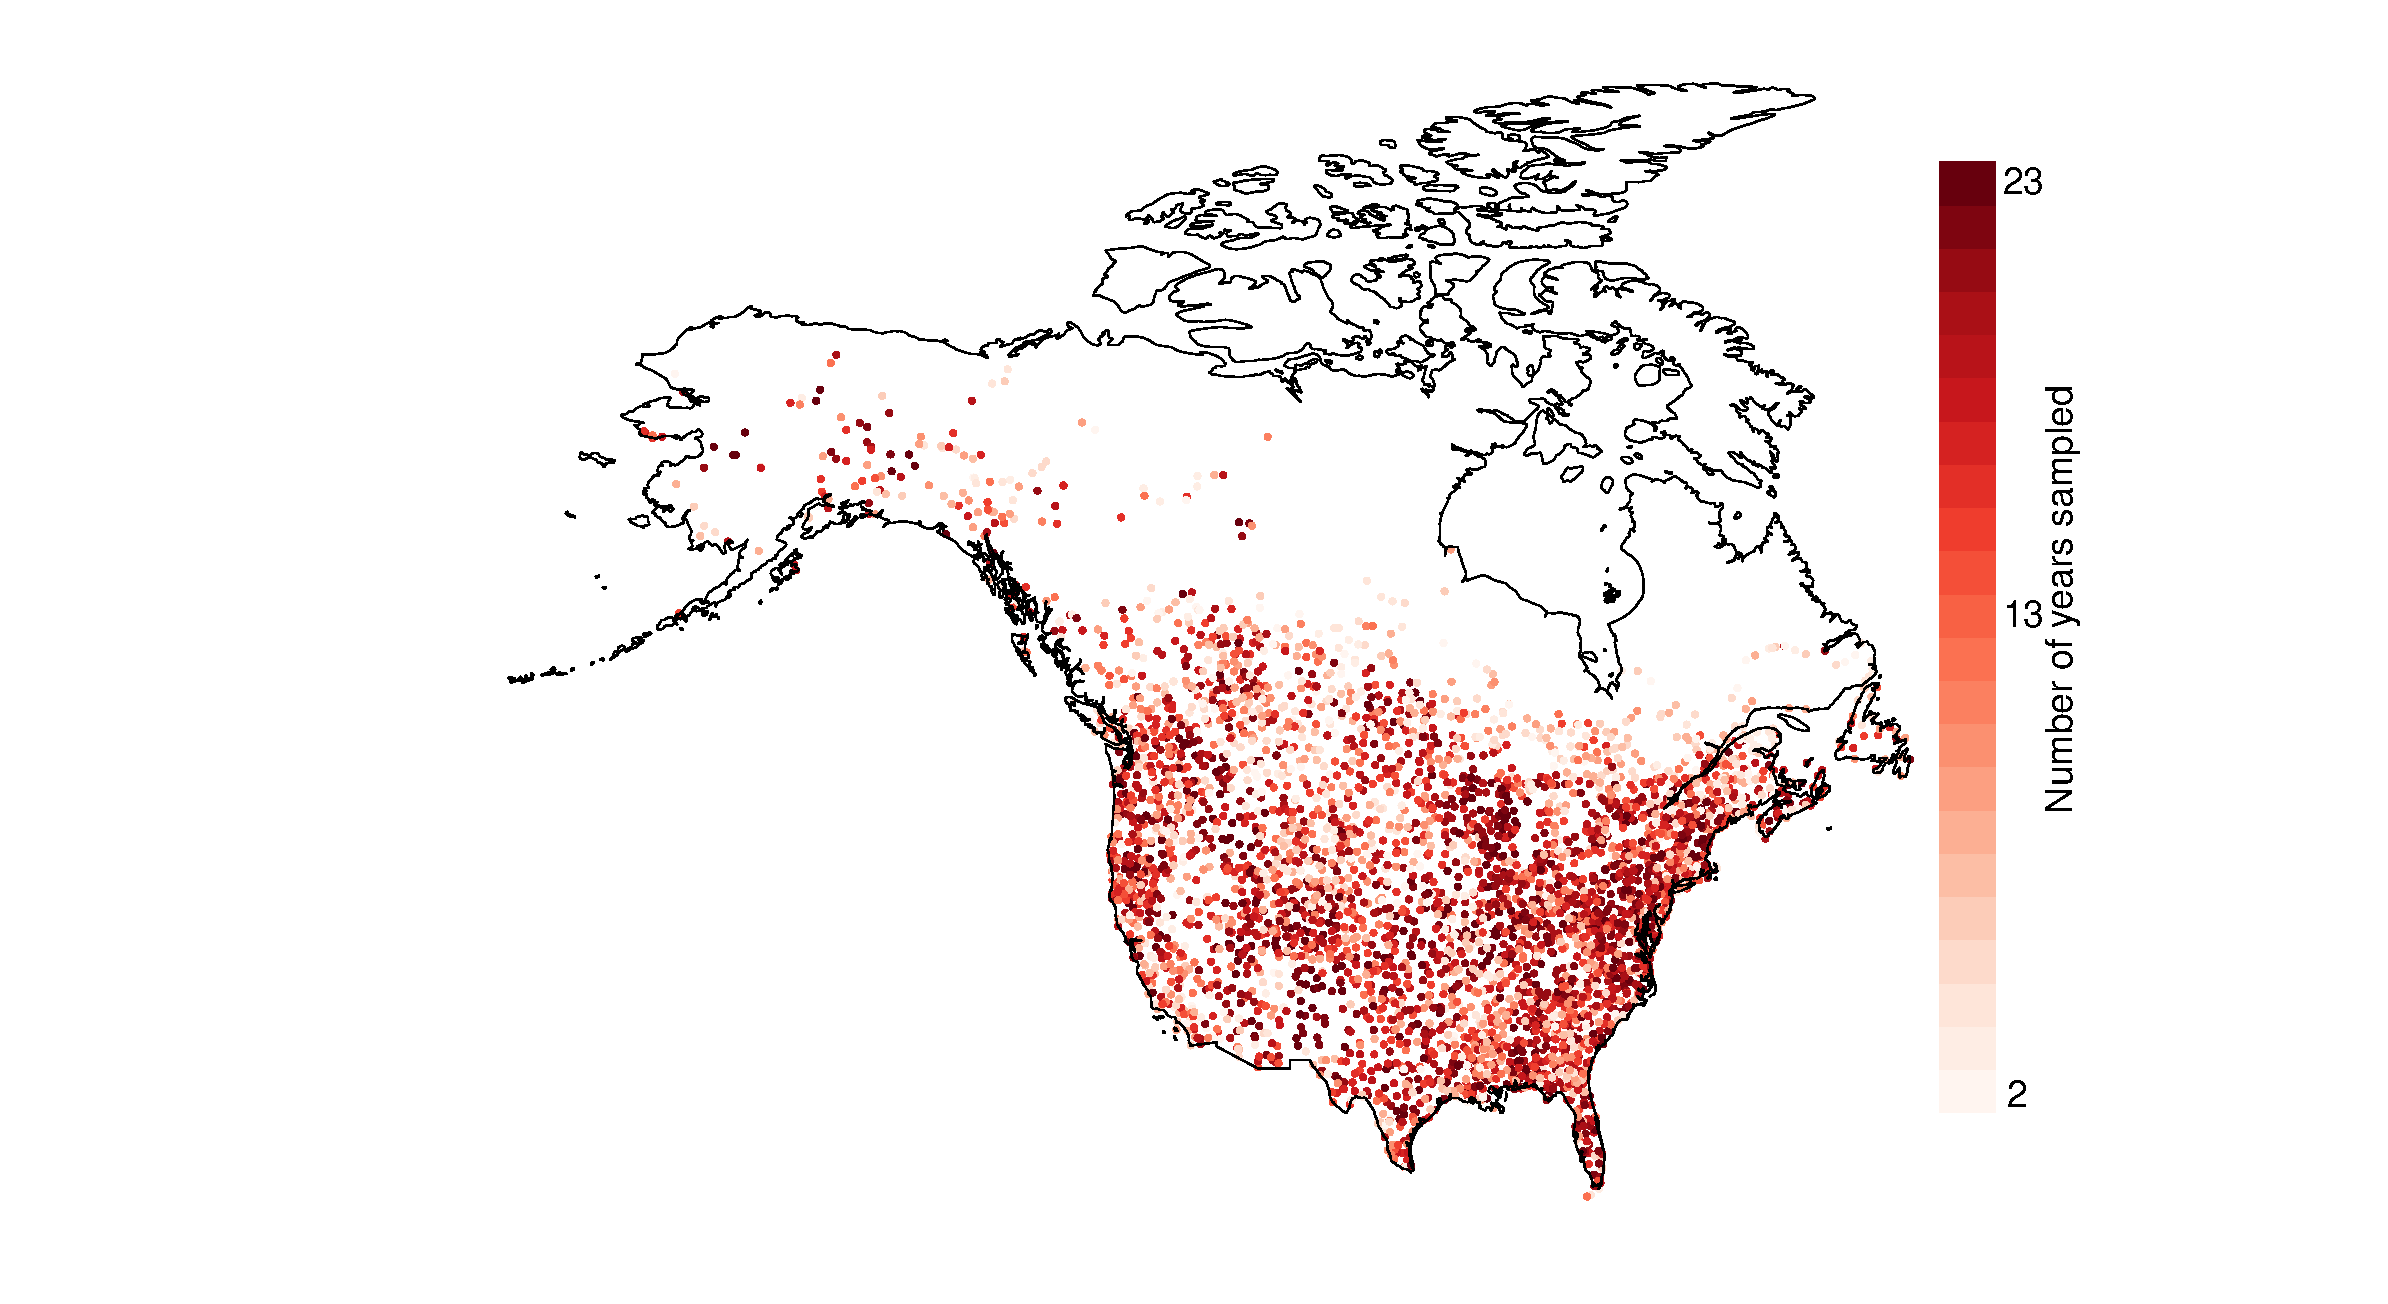
\includegraphics[width=1\textwidth]{FigRange/yearsampled}}
\caption[Routes sampled by the Breeding Bird Survey]{Routes sampled by BBS between 1997 and 2019 where the species used in our analyses occurred. Routes were well sampled during this time period, with an average of $\approx$ 3000 routes sampled yearly. Colors represent the number of years routes were sampled between 1997 and 2019.}  
\label{fig:routes}
\end{figure}
\section*{\textbf{Model diagnostics}}
Model diagnostics for the linear mixed models that we fit were done using the \texttt{performance} R package. We checked model convergence and singularity using the functions \textit{check$\_$convergence} and \textit{check$\_$singularity}. Heteroscedasticity was checked for using the function \textit{check$\_$heteroscedasticity}, which performs the Breusch-Paga test for heteroscedasticity. Overdispersion and underdispersion were checked using the function \textit{check$\_$overdispersion}. Additionally, visual checks were also performed for all models using the \textit{check$\_$model} function. All models that we fit successfully converged, were not singular, had homoscedastic error variance, and were not over or underdispersed. Visual checks also indicated that model assumptions were generally met (Figures \ref{fig:main_mod}-\ref{fig:comp_mod}), suggesting that our results are robust. 

\begin{figure}[H]
\centering
\centerline{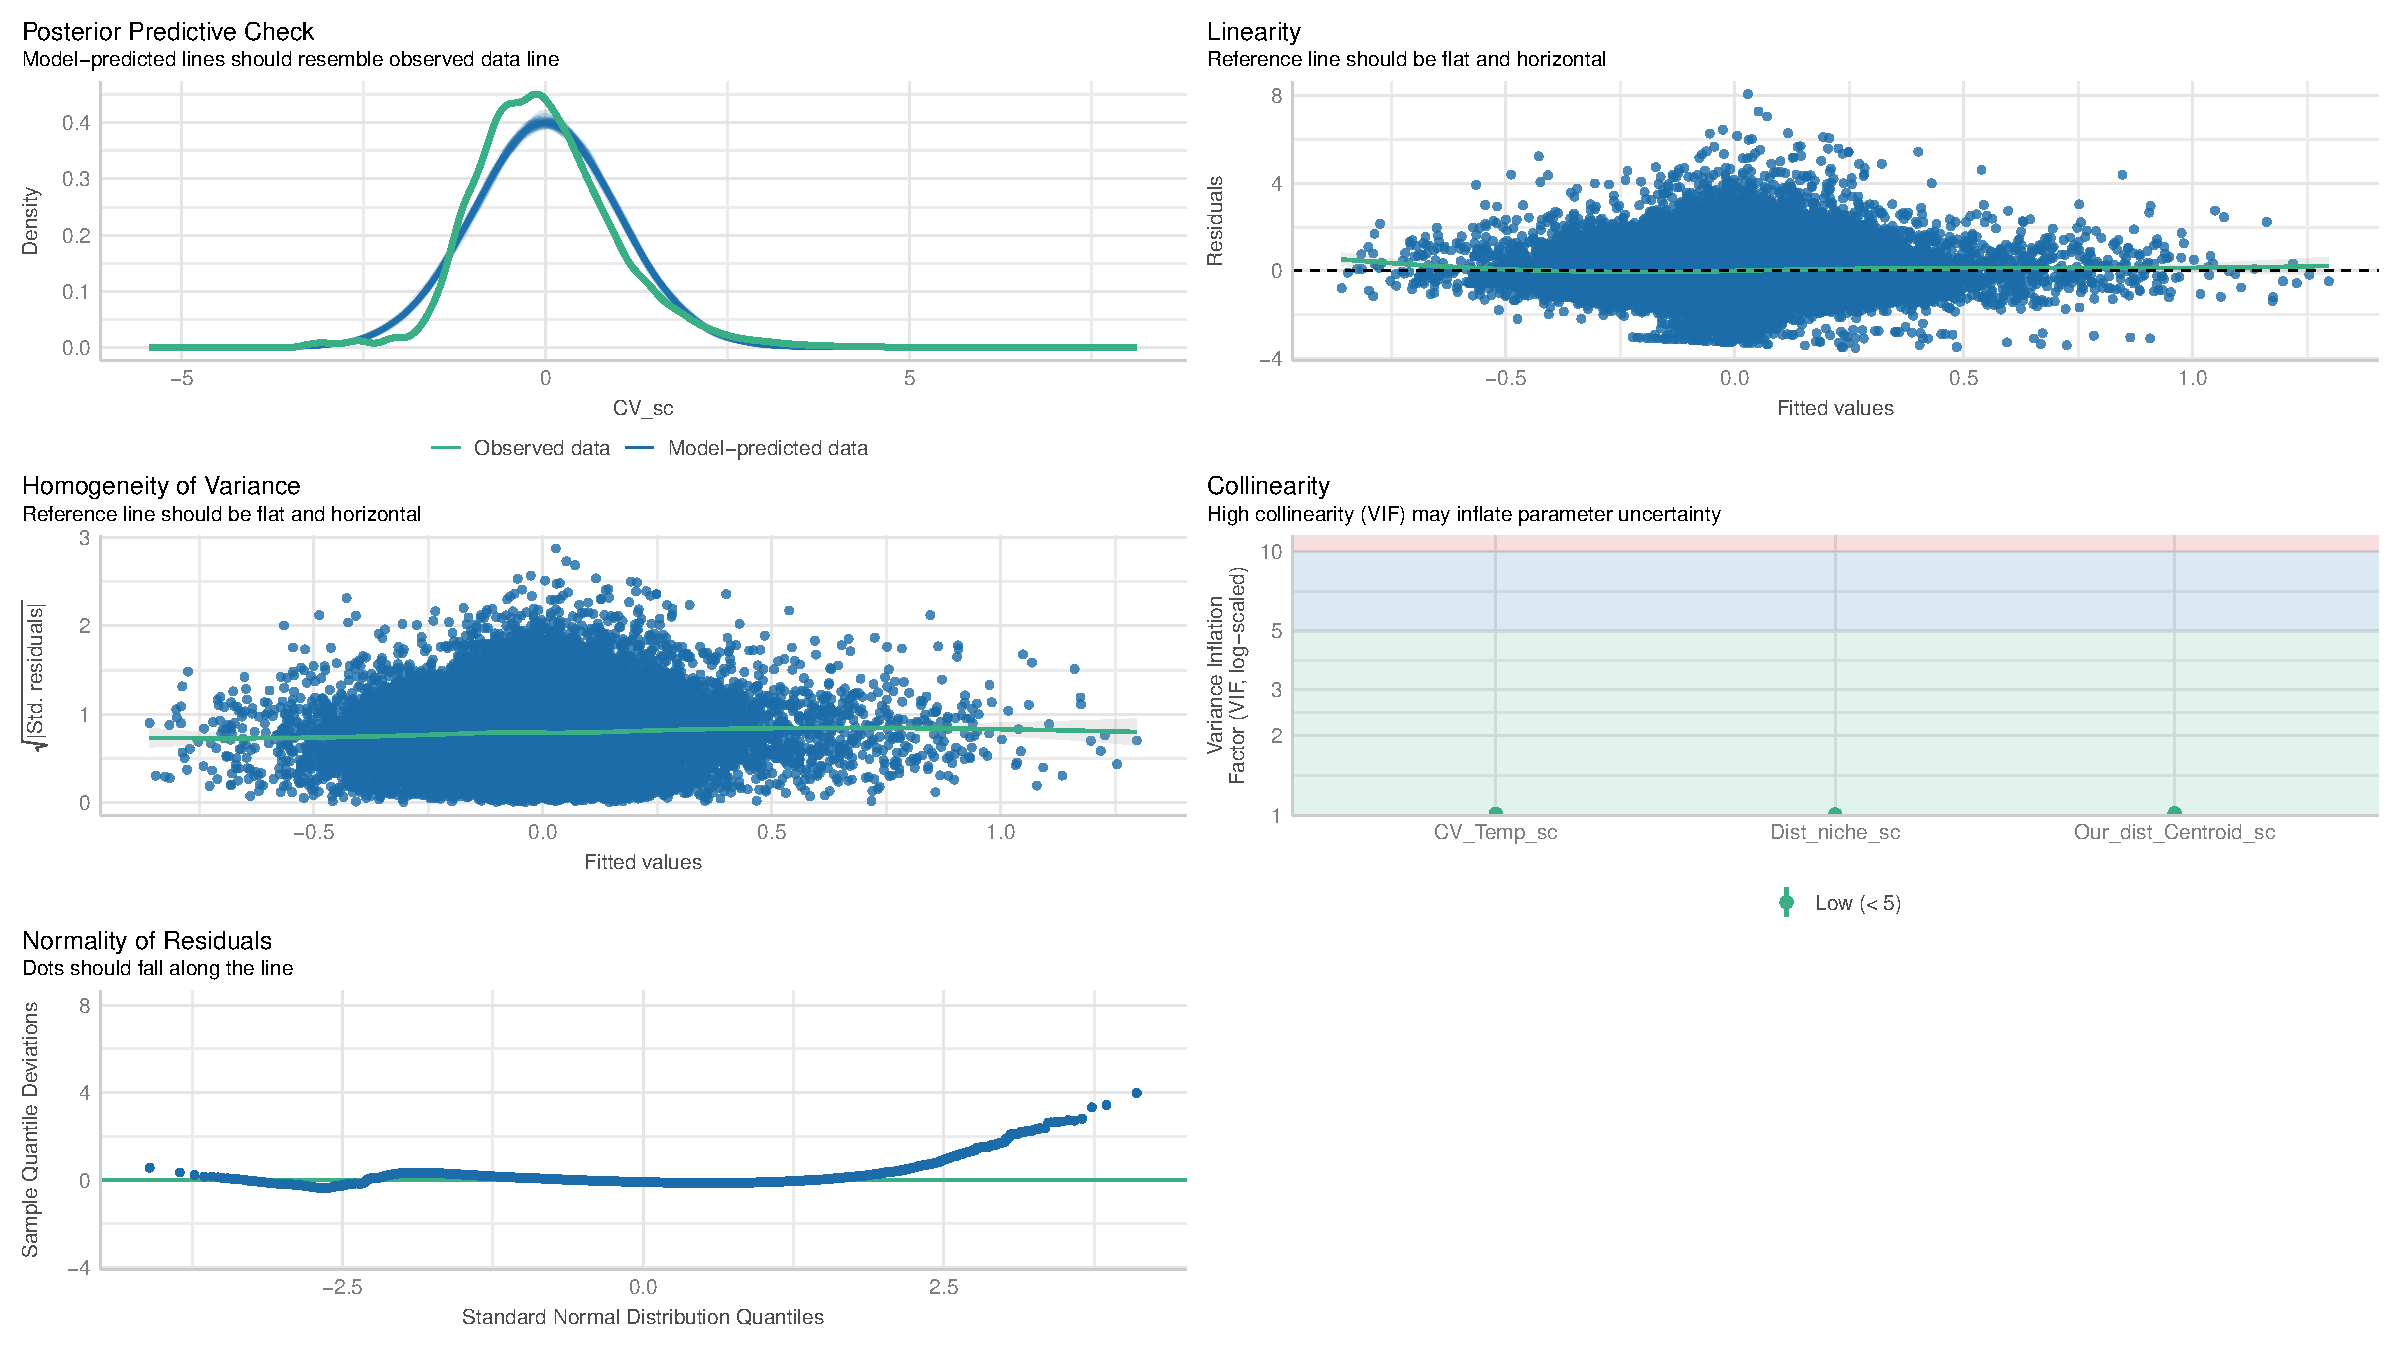
\includegraphics[width=1\textwidth]{FigRange/mod_main}}
\caption[Main model diagnostics]{Visual model diagnostics for the model used to report the results in the main text (Table \ref{tab:lmm_main}). Overall, the gaussian family fits well to the response variable that we used in the models (CV$\_$sc; scaled population variability), the linearity assumption is met, variance is homogeneous, there is not correlation between the predictor variables (i.e., variance inflation factor (VIF) < 5), and the residuals are normally distributed.}  
\label{fig:main_mod}
\end{figure}

\begin{figure}[H]
\centering
\centerline{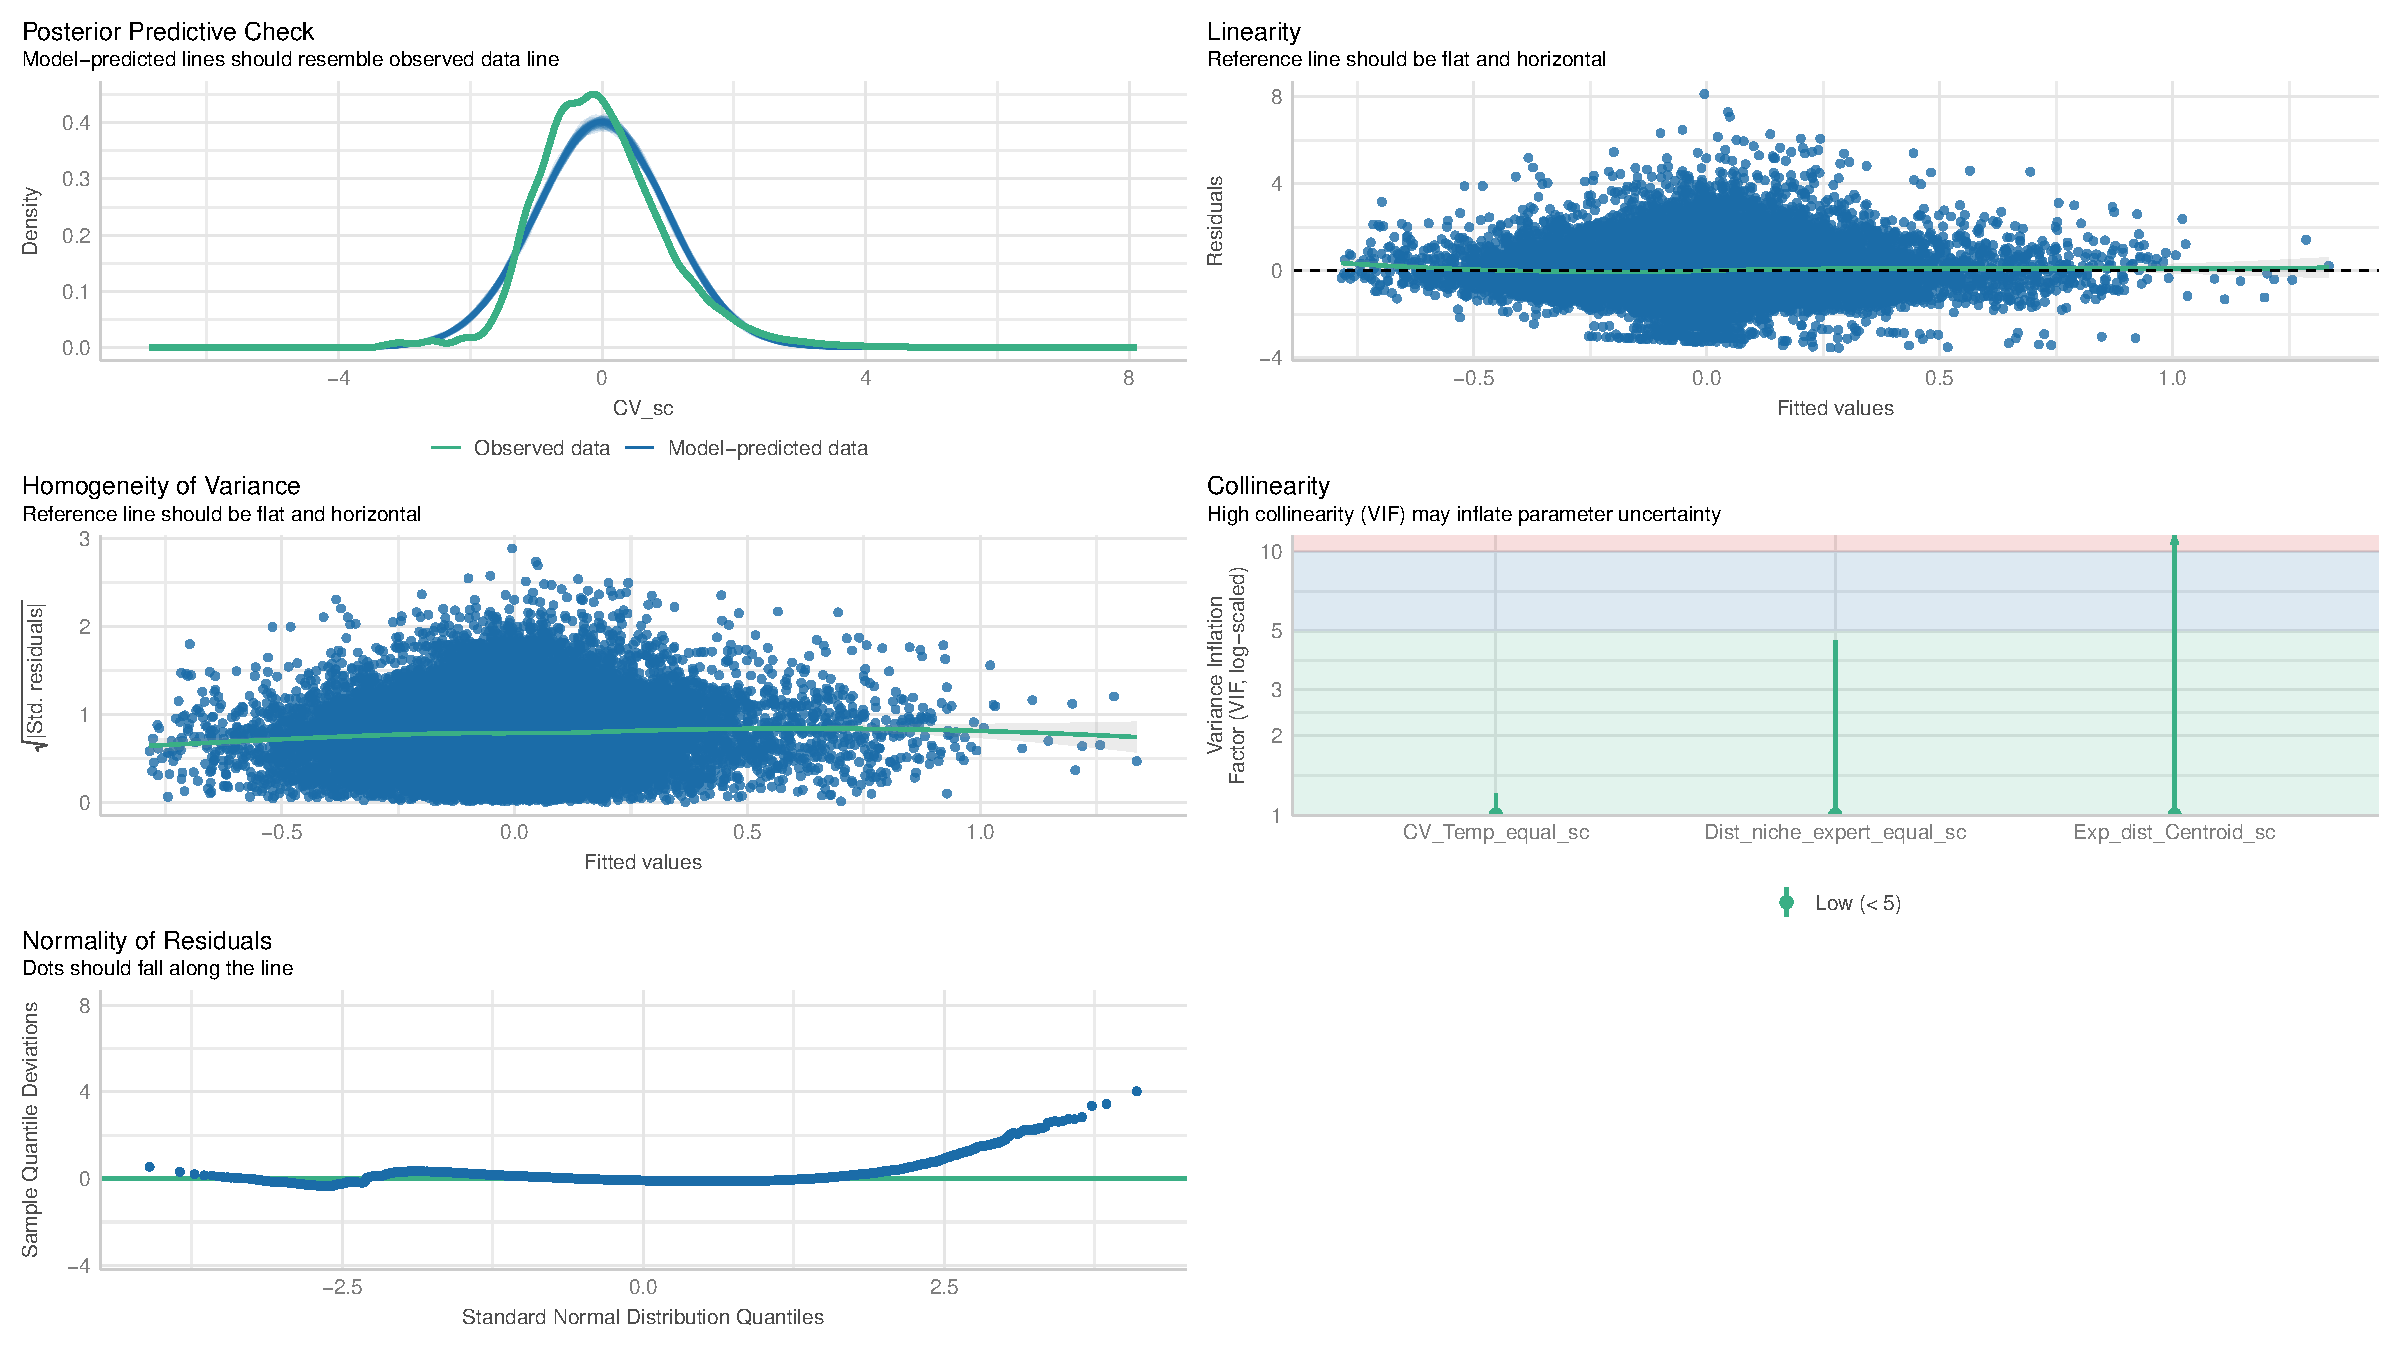
\includegraphics[width=1\textwidth]{FigRange/mod_exp}}
\caption[Expert model diagnostics]{Visual model diagnostics for the model that estimated distance to geographic range center and climatic niche position from expert ranges, and that used temperature variability data aggregated from Behrmann equal area projection, as predictors (Table \ref{tab:lmm_exp}). Overall, the gaussian family fits well to the response variable that we used in the models (CV$\_$sc; scaled population variability), the linearity assumption is met, variance is homogeneous, and there is relatively low correlation between the predictor variables (i.e., variance inflation factor (VIF) often < 5), and the residuals are normally distributed.}  
\label{fig:exp_mod}
\end{figure}

\begin{figure}[H]
\centering
\centerline{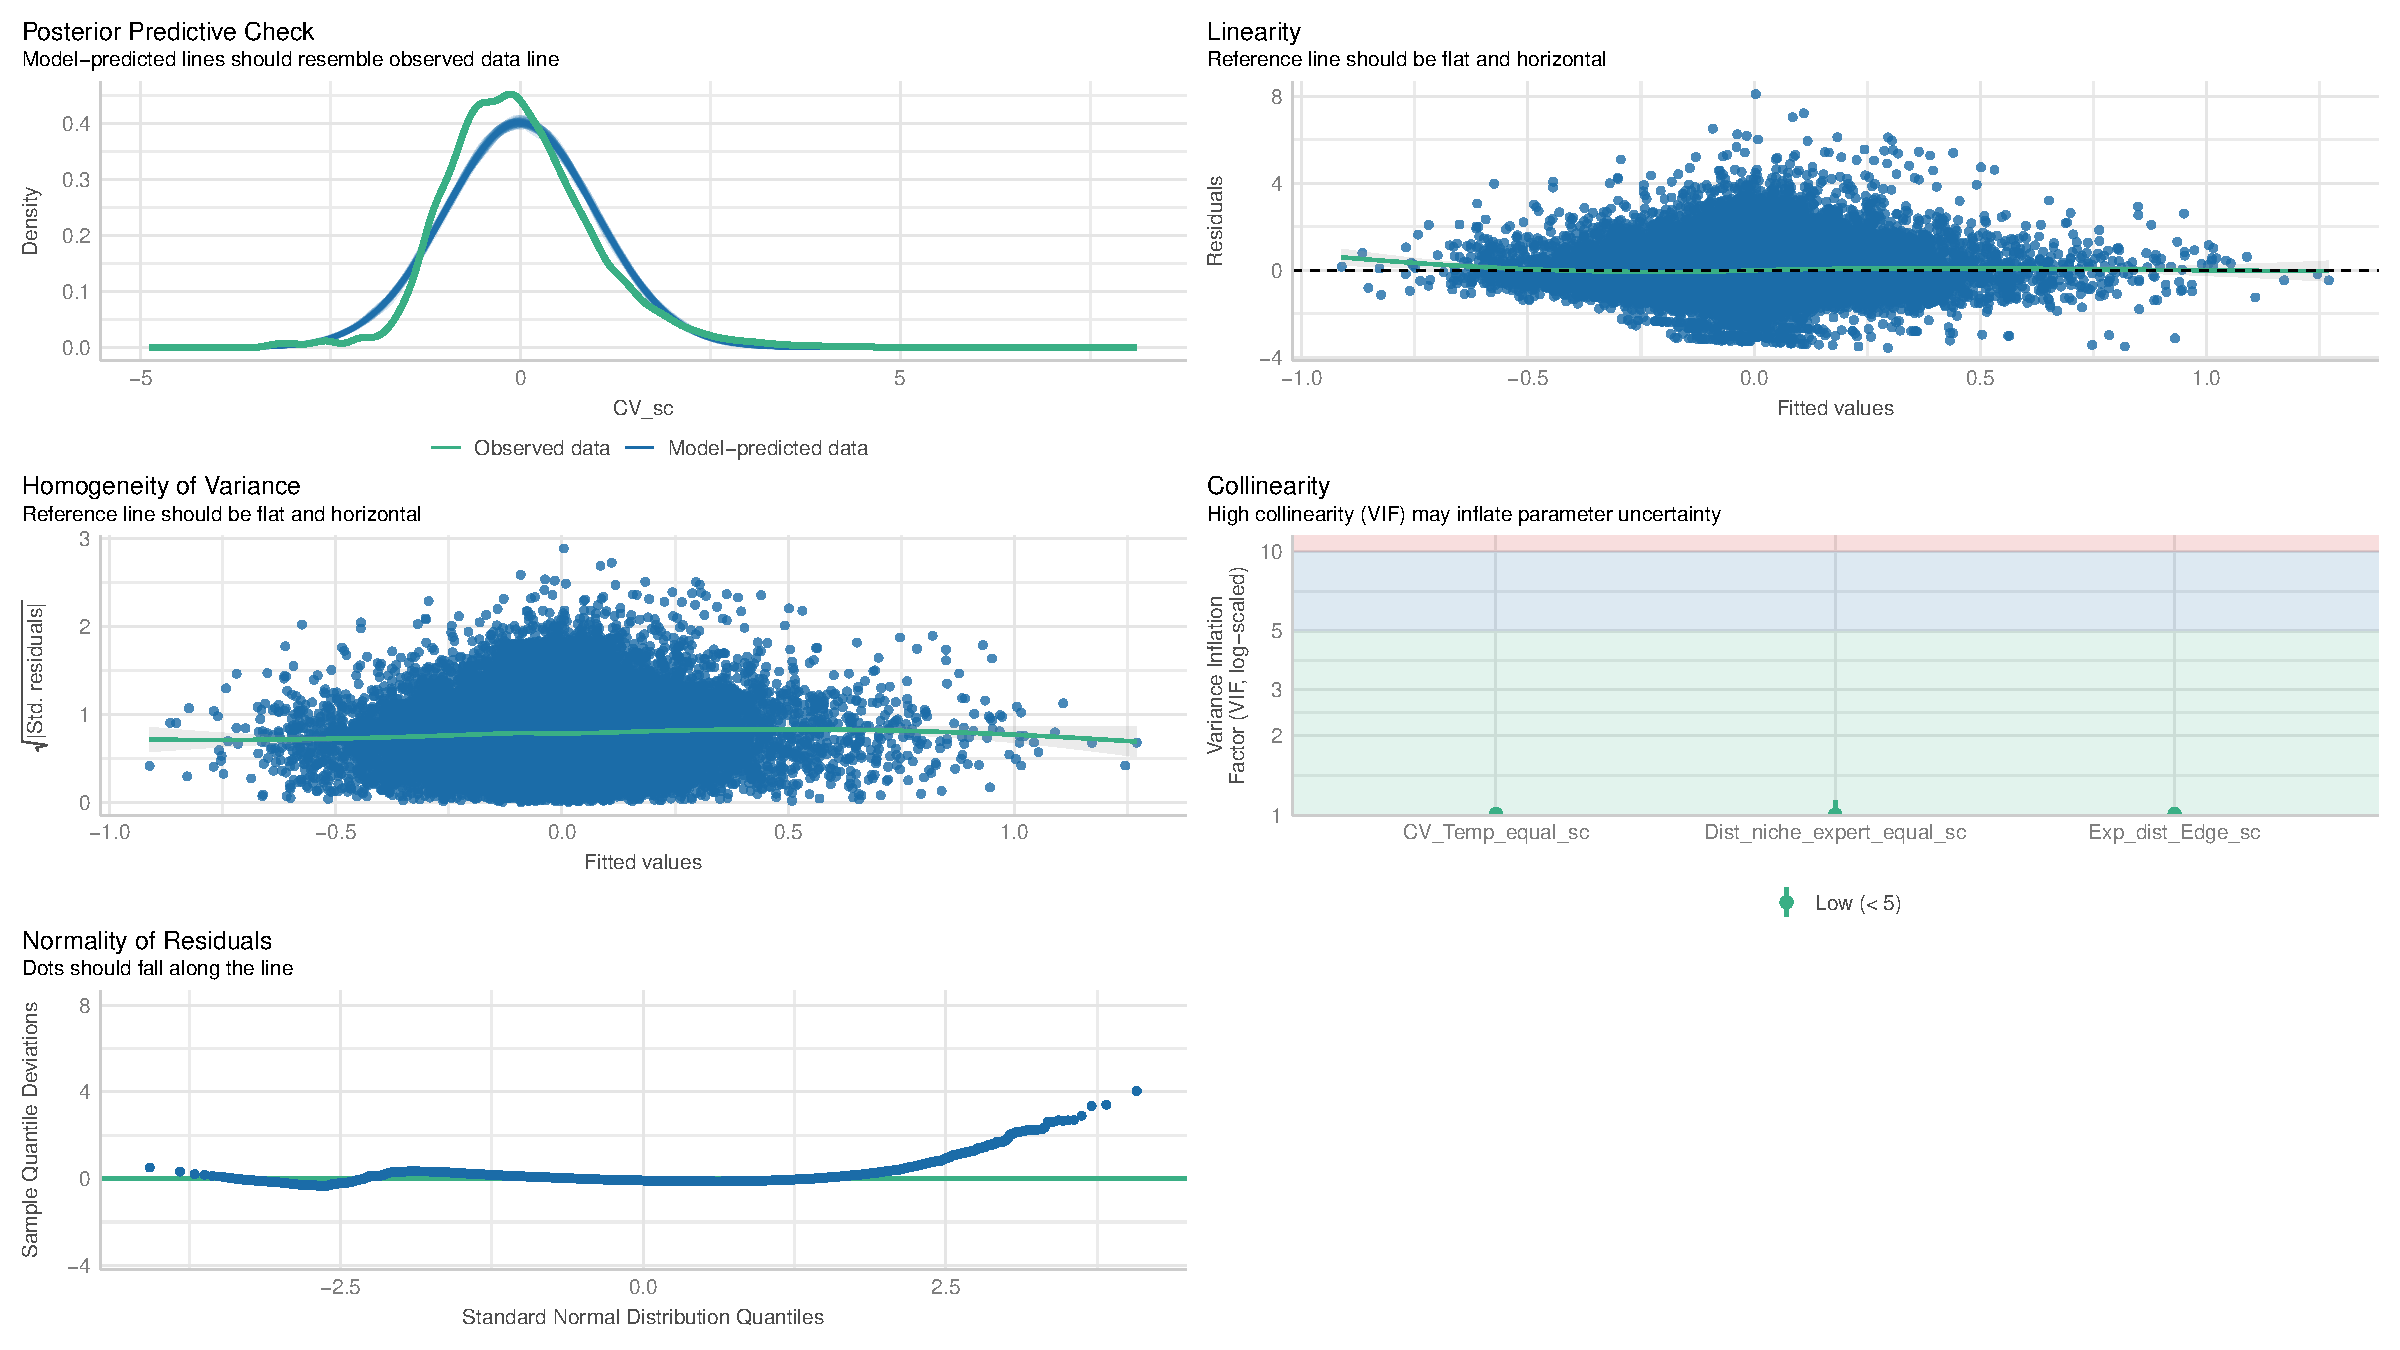
\includegraphics[width=1\textwidth]{FigRange/mod_edge}}
\caption[Edge model diagnostics]{Visual model diagnostics for the model that estimated distance to geographic range edges and climatic niche position from expert ranges, and that used temperature variability data aggregated from Behrmann equal area projection, as predictors (Table \ref{tab:lmm_edge}). Overall, the gaussian family fits well to the response variable that we used in the models (CV$\_$sc; scaled population variability), the linearity assumption is met, variance is homogeneous, and there is low correlation between the predictor variables (i.e., variance inflation factor (VIF) < 5), and the residuals are normally distributed.}  
\label{fig:edge_mod}
\end{figure}

\begin{figure}[H]
\centering
\centerline{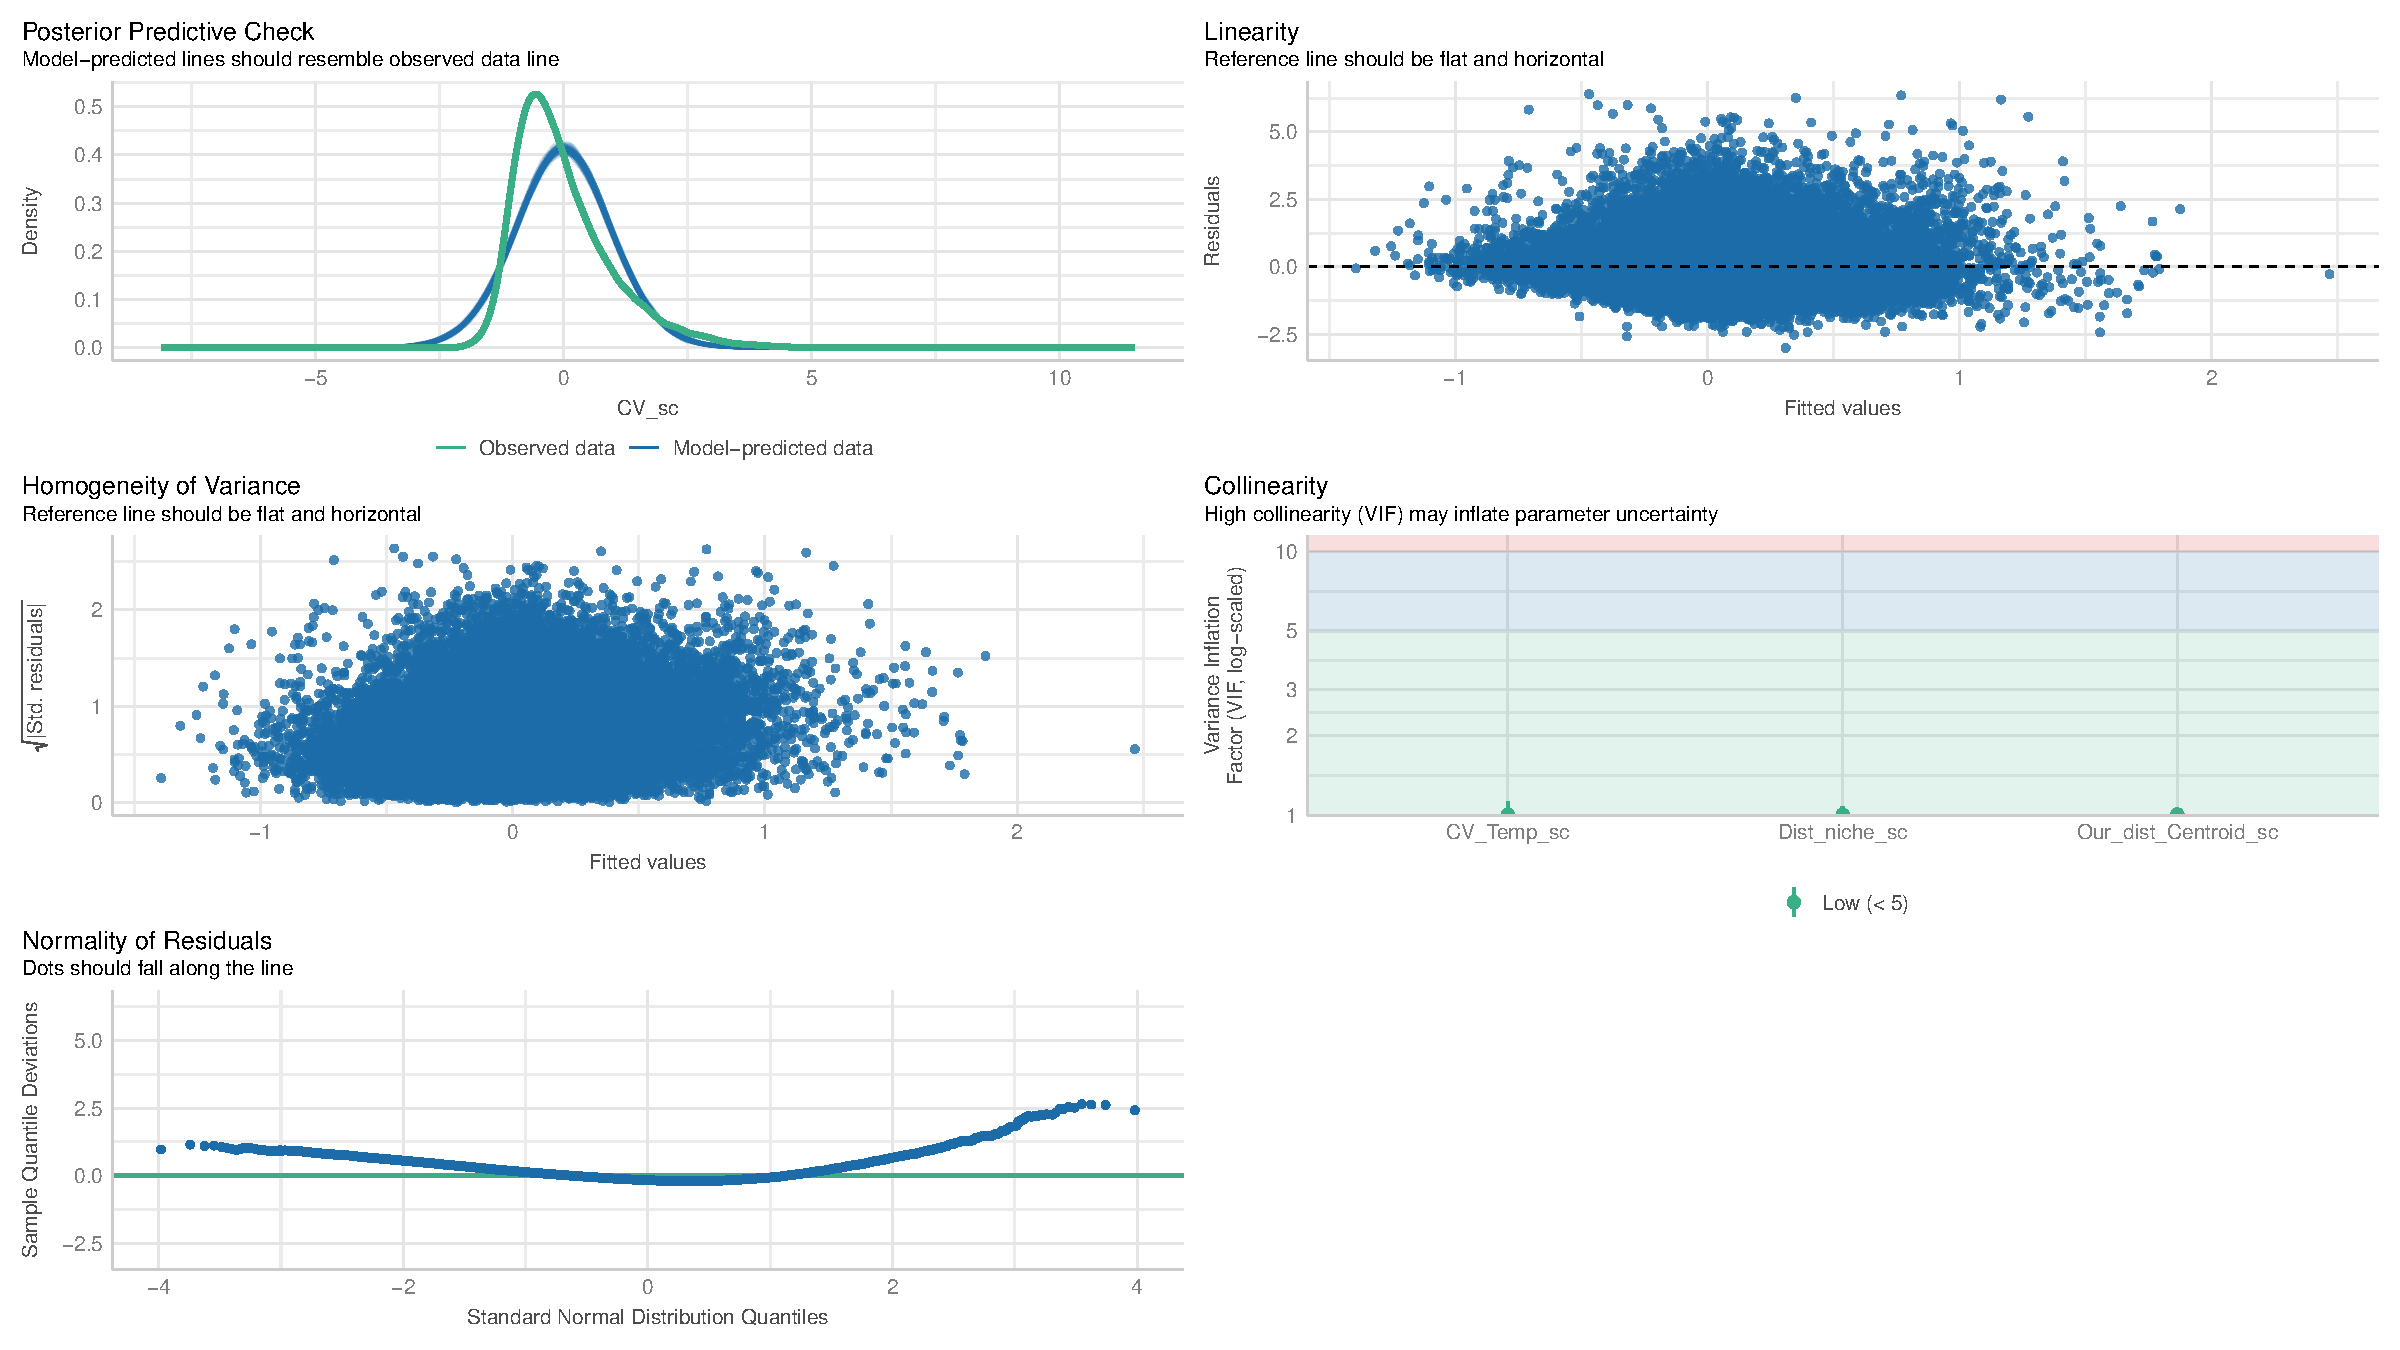
\includegraphics[width=1\textwidth]{FigRange/mod_0s}}
\caption[Zero model diagnostics]{Visual model diagnostics for the model where population variability was estimated considering zeros to years where a species was not recorded in a site, but that sampling event was done between the first and last year that a species was observed at a given site (Table \ref{tab:lmm_zeros}). Overall, the gaussian family fits well to the response variable that we used in the models (CV$\_$sc; scaled population variability), the linearity assumption is met, variance is homogeneous, and there is low correlation between the predictor variables (i.e., variance inflation factor (VIF) < 5), and the residuals are normally distributed.}  
\label{fig:0s_mod}
\end{figure}

\begin{figure}[H]
\centering
\centerline{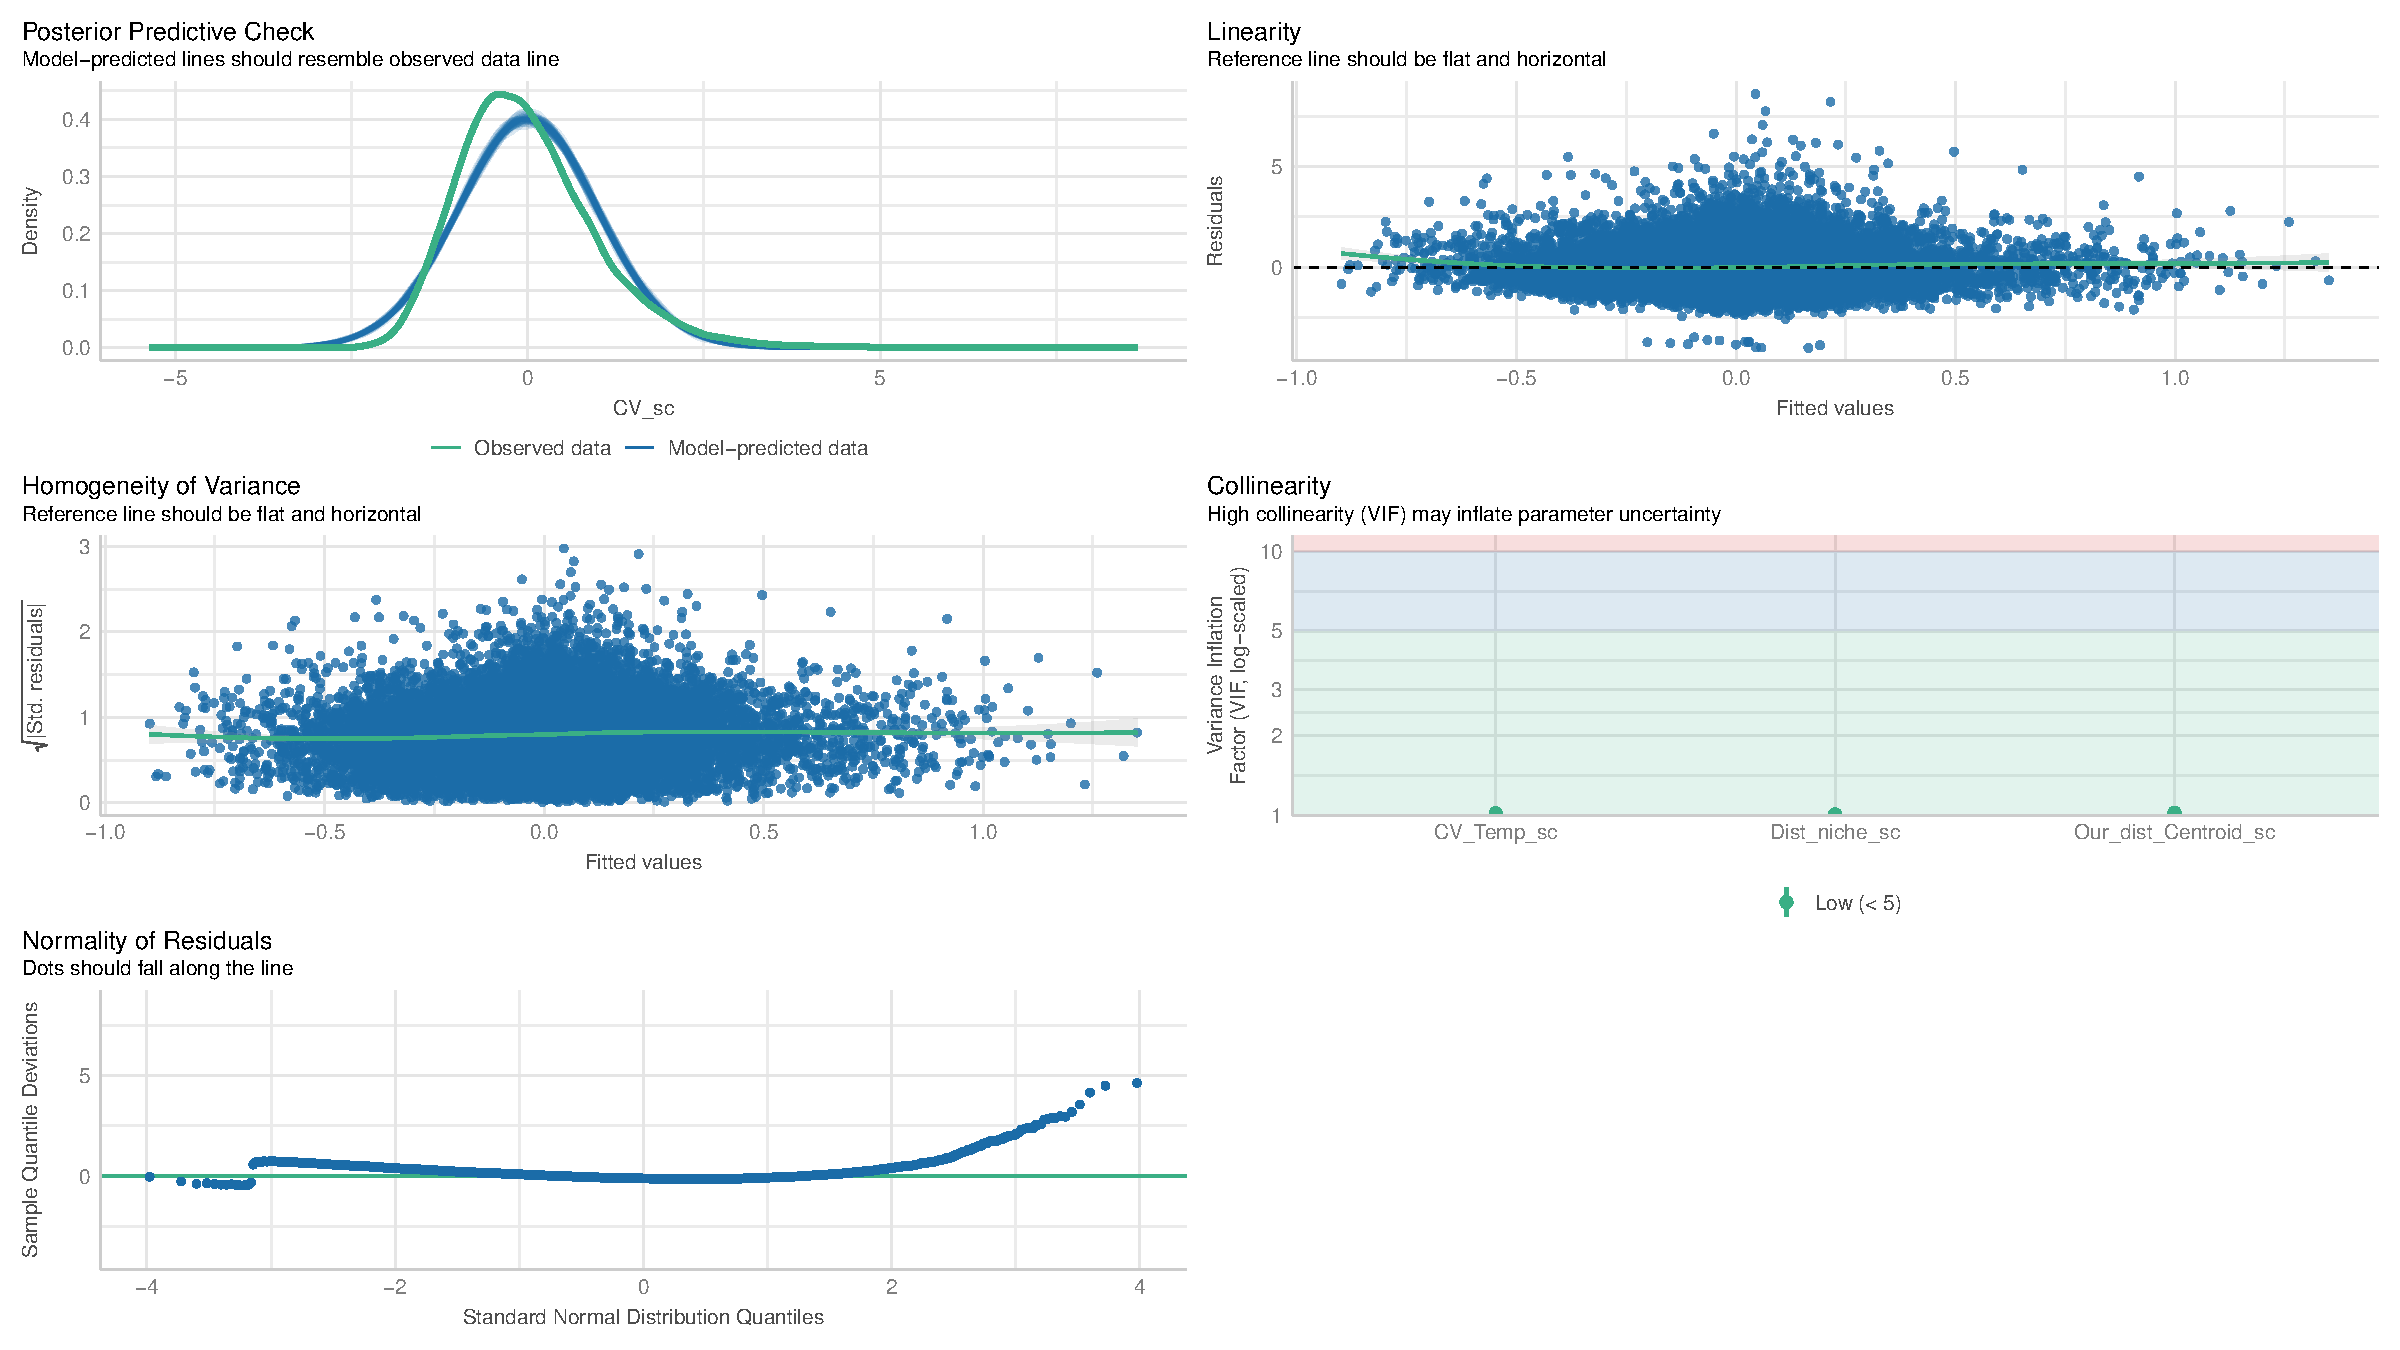
\includegraphics[width=1\textwidth]{FigRange/mod_10}}
\caption[Ten years model diagnostics]{Visual model diagnostics for the model where population variability was estimated considering only sites where species occupied for at least 10 years (Table \ref{tab:lmm_tens}). Overall, the gaussian family fits well to the response variable that we used in the models (CV$\_$sc; scaled population variability), the linearity assumption is met, variance is homogeneous, and there is low correlation between the predictor variables (i.e., variance inflation factor (VIF) < 5), and the residuals are normally distributed.}  
\label{fig:10_mod}
\end{figure}

\begin{figure}[H]
\centering
\centerline{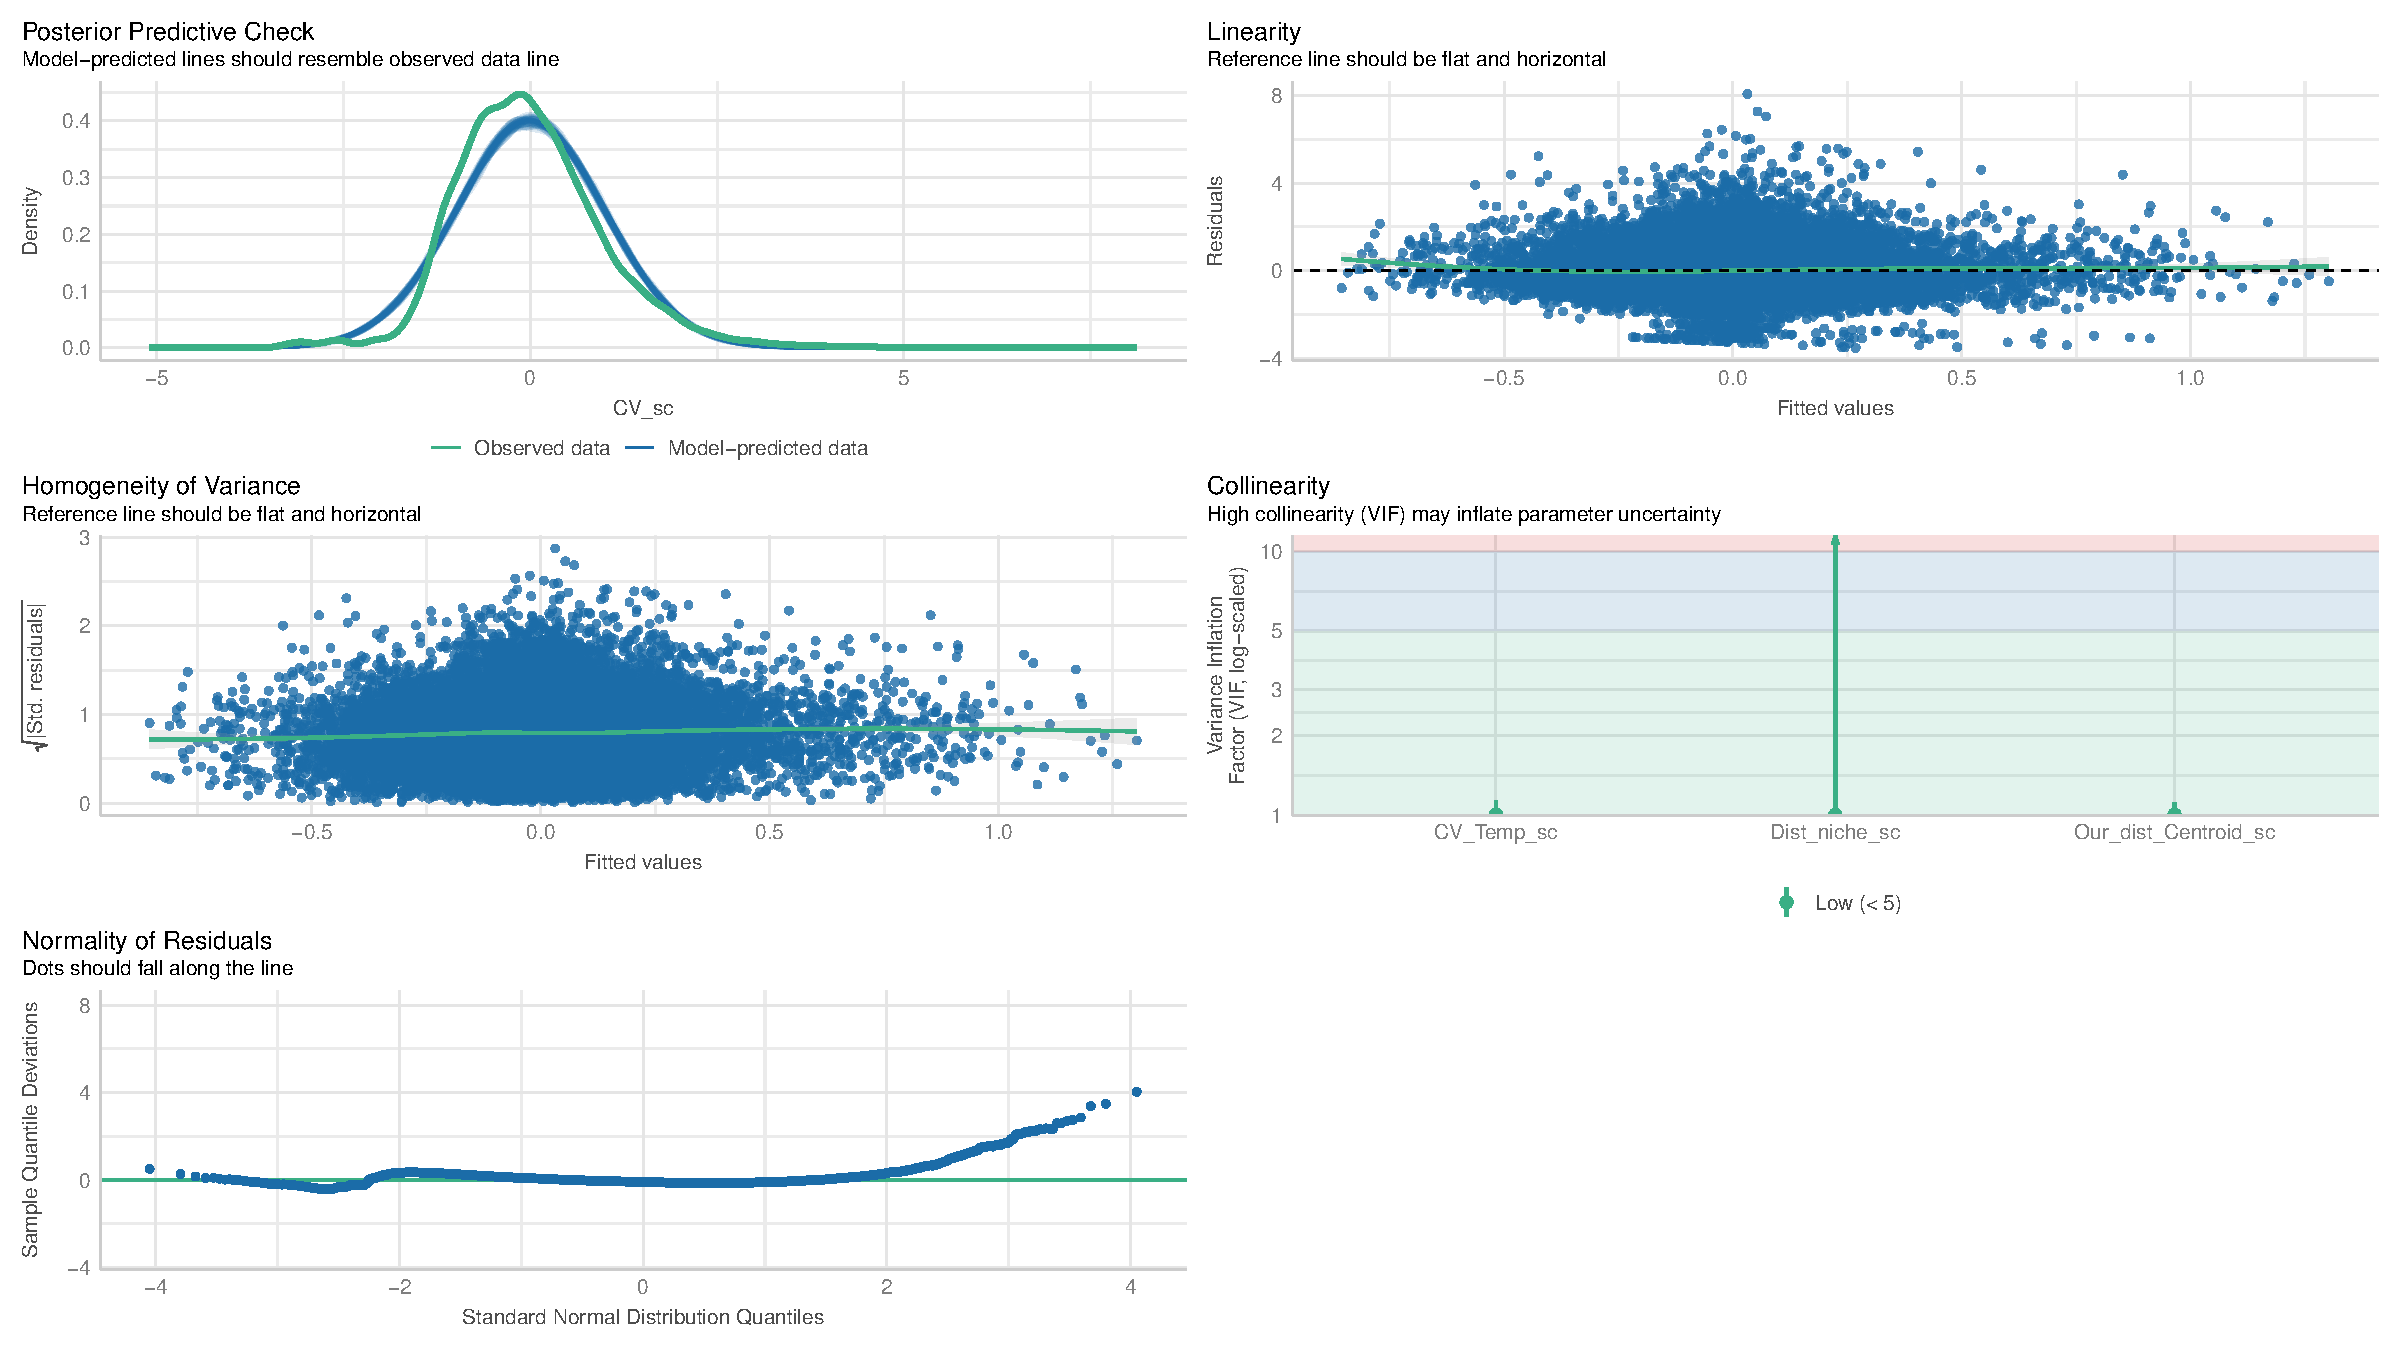
\includegraphics[width=1\textwidth]{FigRange/mod_comp}}
\caption[Range model diagnostics]{Visual model diagnostics for the model where we only considered the species that had $\geq$70\% of their geographic ranges sampled by BBS (Table \ref{tab:lmm_comp}). Overall, the gaussian family fits well to the response variable that we used in the models (CV$\_$sc; scaled population variability), the linearity assumption is met, variance is homogeneous, and there is relatively low correlation between the predictor variables (i.e., variance inflation factor (VIF) often < 5), and the residuals are normally distributed.}  
\label{fig:comp_mod}
\end{figure}

\section*{\textbf{Assessing the robustness of our results to methodological choices}}
Species geographic ranges and climatic niches can be estimated using different approaches that could affect our results. We used expert geographic ranges from birdLife and used these niches to estimate geographic range position and climatic niches. We estimated geographic range position as distance to range center and range edge. We did not estimate distance to geographic range edge for populations falling outside the expert ranges (i.e., these populations were removed from our analyses). The model fit using expert distance to range center considered 96 species (\textit{Aphelocoma woodhouseii} was removed from this analyses because it does not have expert ranges). Alternatively, the model fit using distance to range edge considered 94 species that had at least five populations sampled within their geographic ranges for five or more years. To estimate species climatic niches from expert ranges, we transformed these ranges and the bioclimatic variables (used to perform the PCA) to Behrmann equal area projection. All environmental values that fell within expert ranges were used to estimate species climatic niches. We also estimated temperature variability using Behrmann equal area to account for potentially different number of cells being aggregated across latitudes when estimating population variability for each route sampled by BBS. 
\paragraph*{}
Overall, we found the same results as reported in the main text regardless of how range position, climatic niches and temperature variability was estimated. Specifically, population variability was unrelated to distance to range center (Table \ref{tab:lmm_exp}) or range edge (Table \ref{tab:lmm_edge}) of expert geographic ranges. Population variability increased towards climatic niche limits when expert ranges were used to estimate climatic niches and in sites that had more variable temperatures when temperature was aggregated using equal area projection (Table \ref{tab:lmm_exp}).

% latex table generated in R 4.3.2 by xtable 1.8-4 package
% Wed Jan 22 10:41:08 2025
\begin{table}[ht]
\centering
\caption[Expert mixed effect model results]{Results from the linear mixed model that estimated distance to geographic range centers and climatic niches using expert ranges and temperature variability using Berhmann equal area projection. This model was fit considering 96 species. The results from this model are virtually the same as the results from the model presented in the main text, such that population variability increased towards climatic niche limits (Niche) and in variable temperatures (Temp.), but not near geographic range edges (Range). This model also had low explanatory power (conditional $R^2$ = 0.01). Bold p-values represent significant relationships. } 
  \vspace*{3mm}
\begin{tabular}{ccccc}
  \hline
 Predictor & Estimate & Std. Error & z value & Pr($>$|$z$|) \\ 
  \hline
  Intercept & 0.005 & 0.005 & 0.968 & 0.333 \\ 
  Niche & 0.039 & 0.013 & 2.946 & \textbf{0.003} \\ 
  Range & -0.002 & 0.015 & -0.151 & 0.880 \\ 
  Temp. & 0.037 & 0.014 & 2.688 & \textbf{0.007} \\ 
   \hline
\end{tabular}
\label{tab:lmm_exp}
\end{table}

% latex table generated in R 4.3.2 by xtable 1.8-4 package
% Wed Jan 22 10:53:33 2025
\begin{table}[H]
\centering
\caption[Edge mixed effect model results]{Results from the linear mixed model that estimated distance to geographic range edges and climatic niches using expert ranges and temperature variability using Berhmann equal area projection. This model was fit considering 94 species. The results from this model are virtually the same as the results from the model presented in the main text, such that population variability increased towards climatic niche limits (Niche) and in variable temperatures (Temp.), but not near geographic range edges (Range). This model also had low explanatory power (conditional $R^2$ = 0.01). Bold p-values represent significant relationships. } 
  \vspace*{3mm}
\begin{tabular}{ccccc}
  \hline
 Predictor & Estimate & Std. Error & z value & Pr($>$|$z$|) \\ 
  \hline
  Intercept & 0.004 & 0.005 & 0.768 & 0.442 \\ 
  Niche & 0.043 & 0.014 & 3.110 & \textbf{0.002} \\ 
  Range & 0.000 & 0.013 & 0.024 & 0.981 \\ 
  Temp. & 0.037 & 0.014 & 2.538 & \textbf{0.011} \\ 
   \hline
\end{tabular}
\label{tab:lmm_edge}
\end{table}

%%PASTE TABLES HERE?
\paragraph*{}
In the main text we estimated population variability considering only sites that a species was observed to occur for at least five years. In this case, species absences in sites between the first and last years that they were observed in a site (i.e., a density of zero) were not considered when estimating population variability. Here, we loosen this assumption and assigned a density of zero to sampling events where a species was not recorded in a site, but that sampling event was done between the first and last year that a species was recorded at a given site. Thus, a species observed during two years in a site could still be included in our analyses if that sites was sampled at least three times between the two observations (i.e., this species would have a density of zero for three years and a density > zero for the two years it was recorded). For this model, the 99 resident species were considered for our analyses as they had over five sites sampled for at least five years within their geographic ranges. In this case, we observed the same relationship as reported in the main text between population variability and climatic niche position and temperature variability. However, population variability also increases towards geographic range edges in this model (Table \ref{tab:lmm_zeros}).  This suggests that some sites are only temporally occupied by the species and that including zeros increases population variability in these sites (Figure \ref{fig:temp_occ}) such that patterns of population variability across geographic ranges become more evident in these cases.
%North American birds are shifting their geographic distributions due to recent climate change \citep{lasorte2007, zurell2024, martins2024} and may not have been able to successfully establish populations near range edges or may be more likely to experience local extirpations in these areas \citep{hampe2011,hargreaves2014,boakes2018, angert2020}
% In that case, years that were sampled and that a species  Here, we loosen 
%We also assessed whether the relationship between population variability and geographic range position, climatic niche position, and temperature variability is dependent on how population variability is estimated. 

We also estimated population variability using a more conservative estimate, where only sites species were observed to occur for at least 10 years were considered in the estimation of population variability. For this model, we considered 90 for our analyses that had over five sites sampled for at least five years within their geographic ranges. Similar to the main text results, population variability increased near niche limits and in variable temperatures. However, in this case we also observed that population variability increased towards geographic range edges (Table \ref{tab:lmm_tens}). This result suggests that time series length can be important to detect population variability patterns. Specifically, longer time series are more likely to capture higher variability in population densities that could be caused by different mechanisms. For example, long-term population trends may only be detected with longer time series, but longer time series may also be more likely to capture populations that are recovering from infrequent, but severe, disturbances that causes substantial changes in population densities over time. %This would explain the increase in population variability near range edges that we observed when considering populations that were recorded for at least 10 years in our analyses.

% latex table generated in R 4.3.2 by xtable 1.8-4 package
% Wed Jan 22 11:05:09 2025
\begin{table}[ht]
\centering
\caption[Zero mixed effect model results]{Results from the linear mixed model that assigned a density of zero to sampling events where a species was not recorded in a site to estimate population variability. This model was fit considering 99 species. In this case we observed that population variability increased towards climatic niche limits (Niche), geographic ranges edges (Range) and in variable temperatures (Temp.). This model also had low explanatory power (conditional $R^2$ = 0.05). Bold p-values represent significant relationships.} 
  \vspace*{3mm}
\begin{tabular}{ccccc}
  \hline
 & Estimate & Std. Error & z value & Pr($>$|$z$|) \\ 
  \hline
  Intercept & 0.005 & 0.005 & 1.036 & 0.300 \\ 
  Niche & 0.072 & 0.016 & 4.411 & \textbf{<0.001} \\ 
  Range & 0.063 & 0.017 & 3.640 & \textbf{<0.001} \\ 
  Temp. & 0.159 & 0.019 & 8.273 & \textbf{<0.001} \\ 
   \hline
\end{tabular}
\label{tab:lmm_zeros}
\end{table}


% latex table generated in R 4.3.2 by xtable 1.8-4 package
% Wed Jan 22 10:58:34 2025
\begin{table}[ht]
\centering
\caption[Ten years mixed effect model results]{Results from the linear mixed model that only considered sites where species were observed for 10 years to estimate population variability. This model was fit considering 90 species. In this case we observed that population variability increased towards climatic niche limits (Niche), geographic ranges edges (Range) and in variable temperatures (Temp.). This model also had low explanatory power (conditional $R^2$ = 0.02). Bold p-values represent significant relationships. } 
  \vspace*{3mm}
\begin{tabular}{ccccc}
  \hline
 Predictor & Estimate & Std. Error & z value & Pr($>$|$z$|) \\ 
  \hline
  Intercept & 0.025 & 0.007 & 3.876 & \textbf{<0.001} \\ 
  Niche & 0.078 & 0.015 & 5.044 & \textbf{<0.001} \\ 
  Range & 0.036 & 0.014 & 2.512 & \textbf{0.012} \\ 
  Temp. & 0.081 & 0.018 & 4.411 & \textbf{<0.001} \\ 
   \hline
\end{tabular}
\label{tab:lmm_tens}
\end{table}

\begin{figure}[H]
\centering
\centerline{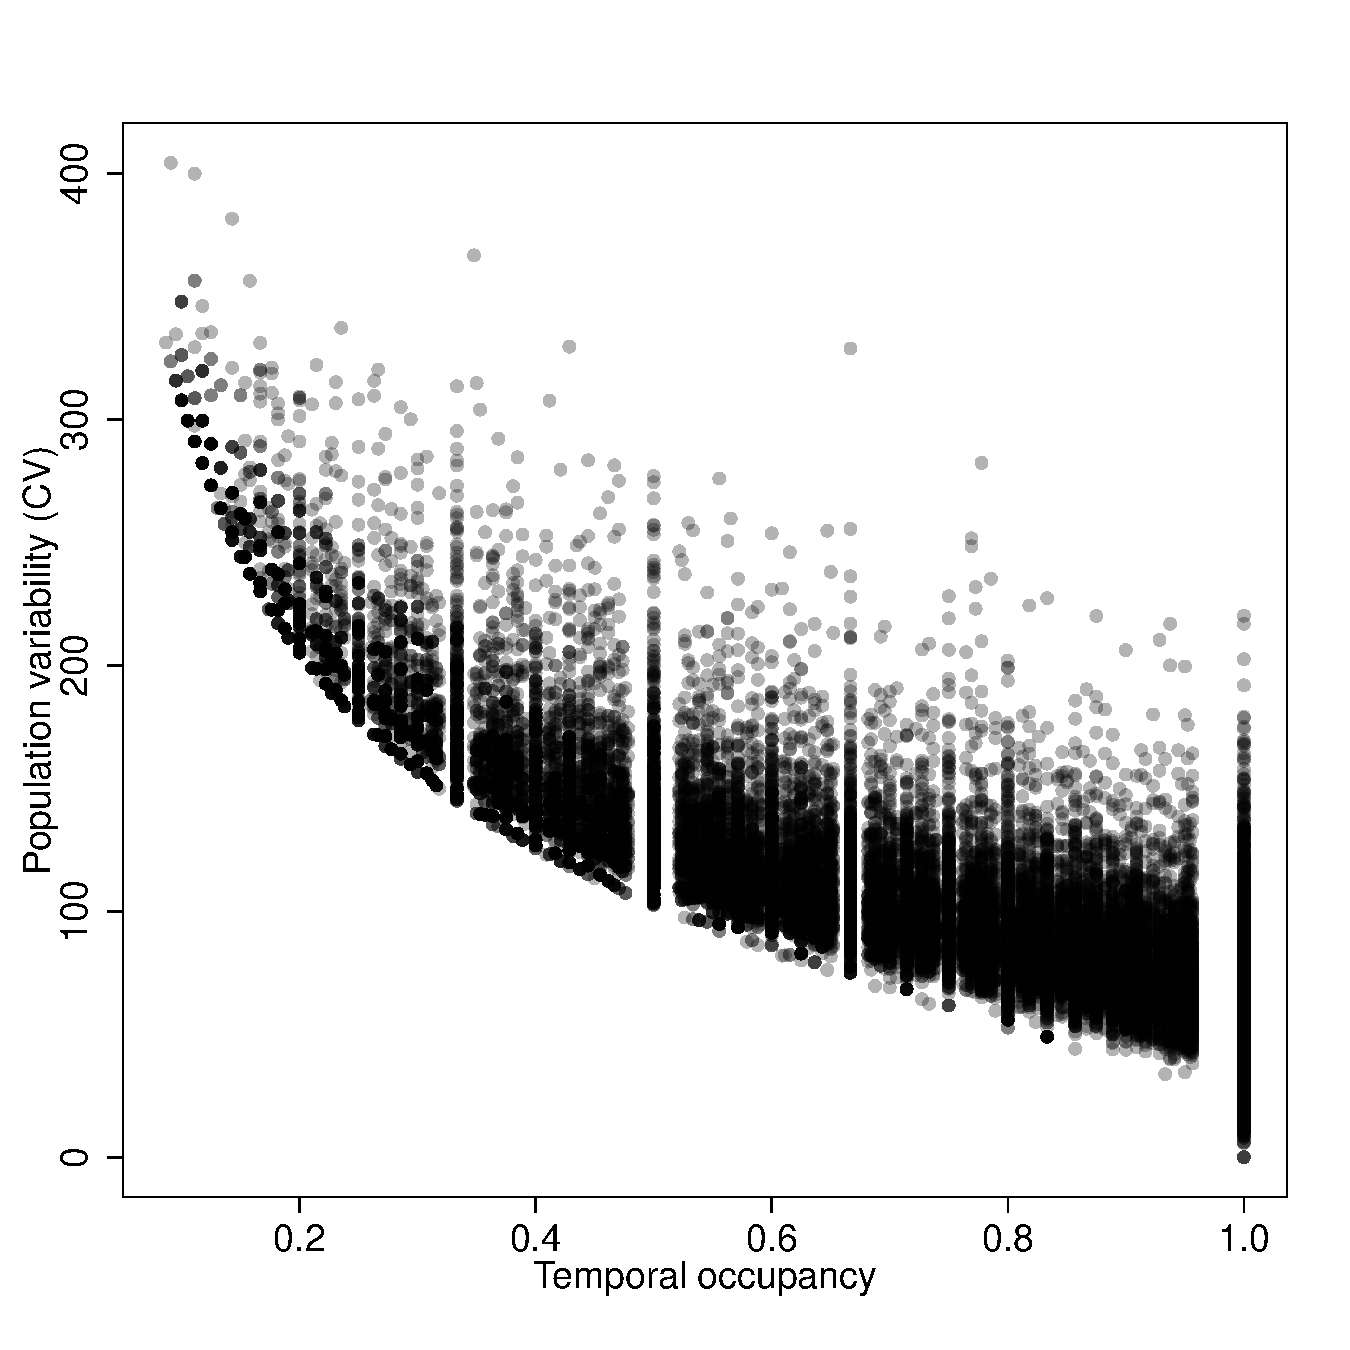
\includegraphics[width=1\textwidth]{FigRange/temp_occ}}
\caption[Temporal occupancy]{There is a strong relationship ($r$ = 0.90, $p < 0.001$) between population variability and population temporal occupancy in a site when zeros are considered during the estimation of population variability.}  
\label{fig:temp_occ}
\end{figure}

In the main text we evaluated the relationship between population variability and geographic range position, climatic niche position, and temperature variability using 97 resident bird species. Here, we restricted our analysis to consider only the species ($n = 52$) that had $\geq$70\% of their geographic ranges sampled by BBS to assess whether our results could have been affected by species that only have a small portion of their range sampled by BBS.  We found the same results as the ones reported in the main text, where popualtion variability increases towards climatic niche limits and in variable temperatures, but not near geographic range edges (Table{\ref{tab:lmm_comp}}. This indicates that considering resident species that have a small portion of their range sampled by BBS did not affect our results.


% latex table generated in R 4.3.2 by xtable 1.8-4 package
% Wed Jan 29 10:54:29 2025
\begin{table}[ht]
\centering
\caption[Range mixed effect model results]{Results from the linear mixed model that only considered species that had $\geq$70\% of their geographic ranges sampled by BBS. This model was fit considering 52 species. The results from this model are virtually the same as the results from the model presented in the main text, such that population variability increased towards climatic niche limits (Niche) and in variable temperatures (Temp.), but not near geographic range edges (Range). This model also had low explanatory power (conditional $R^2$ = 0.01). Bold p-values represent significant relationships.} 
\vspace*{3mm}
\begin{tabular}{ccccc}
  \hline
 & Estimate & Std. Error & z value & Pr($>$|$z$|) \\ 
  \hline
  Intercept & 0.010 & 0.006 & 1.681 & 0.093 \\ 
  Niche & 0.053 & 0.016 & 3.370 & \textbf{0.001} \\ 
  Range & 0.026 & 0.016 & 1.583 & 0.113 \\ 
  Temp. & 0.057 & 0.019 & 3.029 & \textbf{0.002} \\ 
   \hline
\end{tabular}
\label{tab:lmm_comp}
\end{table}
        
\addtocontents{toc}{\protect\vskip-20pt}
\chapter{Rights to reprint work published under a CC-BY 4.0 license}
\begin{figure}[h!]
\centering
\centerline{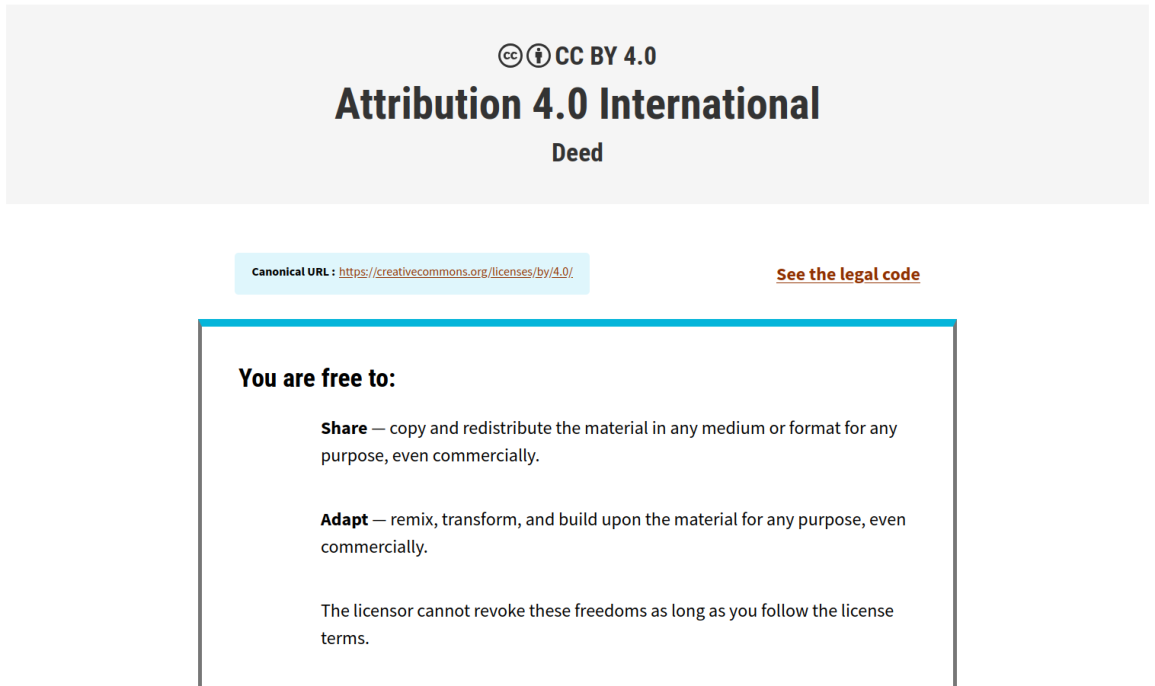
\includegraphics[width=1\textwidth]{FigCC/cc40}}
\caption[Rights to reprint open-access material]{Material that has been previously published under a CC-BY 4.0 license can be reprinted when appropriate credit is given.}
\label{fig:cc40}
\end{figure}

Chapters 2 was published under a CC-BY 4.0 license at the time of preparation of this dissertation. This license allows the reprinting of any previously published material for non-commercial use. Law regarding this license can be read here: \url{https://creativecommons.org/licenses/by/4.0/legalcode.en}
\end{document}
%%%%%%%%%%%%%%%%%%%%%%%%%%%%%%%%%%%%%%%%%%%%%%%%%%%%%%%%%%%%%%%
